% Draft Version 1 - Date 16/06/2020
% Draft Version 2 - Date 06/08/2020
% Draft Version 3 - Date 27/08/2020
% Draft Version 4 - Date 14/12/2020
\captionsetup[subfigure]{labelfont=bf,textfont=normalfont,font=footnotesize}
\makeatletter
\newtheorem{thm}{\protect\theoremname}
\makeatother
\providecommand{\theoremname}{Theorem}
\providecommand{\keywords}[1]{\textbf{\textit{Index terms---}} #1}
\chapter[\titleof]{\titleof\footnote{Sections \ref{of-gen}, \ref{of-feature}, \ref{of-sharp} and \ref{of-fem} of this chapter are adapted from the initial sections of the paper "N. G. Kilingar, K. Ehab Moustafa Kamel, B. Sonon, T. J. Massart, and L. Noels.	\textit{Computational generation of open foam representative volume elements with morphological control using distance fields.} European Journal of Mechanics - A/Solids, page 103847, September 2019."}}\label{chap-of}


\section{Introduction}

Idealization of the open foam micro-structure geometry provides an important class of models that helps exploring the elementary mechanisms strongly related to the morphology of the material. Highly deterministic models based on observations from liquid foams have been studied. The Kelvin model \cite{thomsonLXIIIDivisionSpace1887} consists of a regular packing of slightly curved tetrakaidecahedra cells, for which the aim was to partition a three-dimensional space with minimum partitional area. This was next improved by the Weaire-Phelan foam \cite{weaireCounterexampleKelvinConjecture1994}. A simplistic model made of rectangular prisms was proposed in \cite{gibsonCellularSolidsStructure1997}. These models contain a high degree of periodicity, and are thereby not able to capture the influence of the micro-structural features on the mechanical properties due to the high degree of randomness in the real micro-structures. An analysis of a tetrakaidecahedron unit cell-based computational micro-mechanics model with added imperfections was studied in \cite{wanExperimentalComputationalMicromechanical2015} which predicted values that were in good agreement with the experimental data during the elastic response and the plateau stage. But even then, this geometry is not a reliable comparison as the cell irregularity features were assumed.

The effect of variations on the overall mechanical properties caused by disorder in cellular solids induced by 'imperfections' with respect to an ideal structure required the introduction of complex three-dimensional random models to improve predictions \cite{grenestedtInfluenceCellShape1998}. Random models of open foams inspired from a Vorono\"i tessellation of space based on the distributions of the nuclei \cite{vanderburgLinearElasticProperties1997}, or based on its weighted form called Laguerre tessellation \cite{fanSimulationPolycrystallineStructure2004,lautensackFittingThreedimensionalLaguerre2008}, were found to yield more realistic and versatile representations. Laguerre tessellations generated by random packings of spheres fitted to a given foam require an understanding of the dependence of geometric characteristics of the cells of the model on parameters such as the volume fraction (loosely packed or densely packed), or the radius distribution of the sphere packing (normal distribution, log-normal distribution, gamma distribution,...). 

A wide range of sphere packing algorithms, like force biased algorithm or Jodrey-Tory gravitational algorithm, both classified under collective rearrangement, sedimentation algorithms, or sequential addition methods, exist to simulate spheres packings \cite{bezrukovStatisticalAnalysisSimulated2002}. Studies have also targeted the understanding of  the effect of surface minimization principles to obtain equilibrated shapes in the foam model with Plateau borders undergoing topological evolutions on Laguerre tessellations using the Surface Evolver software \cite{kraynikStructureRandomMonodisperse2003,kraynikStructureRandomFoam2004,kraynikStructureRandomFoam2006,vecchioImprovedModelsSolid2016}. These generation methods are able to properly represent the foam morphological parameters like the cell size distribution, the face-by-cell count, and the edge-by-face count. However, the tessellations cannot represent local morphological features related to the strut, like the strut cross-sections shape, variation and curvature, the coating over the strut, or the presence of hollow struts. The existence of partially reticulated (intermediate state between completely open and closed foams) cannot be accounted for using simple tessellations, requiring further constructions \cite{jangMicrostructureOpencellFoams2008}. %FIGURE MAYBE
Depending on the process used and on requirements, open foam materials are produced with varying strut cross-section, ranging from concave plateau borders to circular shapes that result in the increase of the relative density and variation of cross-section along their length with more material at the nodes \cite{jangMicrostructureOpencellFoams2008}. 

The morphological values of the foam seem to depend on the source and the manufacturing process involved to obtain these samples and hence, a lot of variations can be found in existing publications in their quantification. It is thus of interest to implement a generation tool that can be versatile in its use and take into account these variations. For example, the porosity of the foam decreases with an increase in the pores per inch (ppi) value of the foam under study \cite{jungMicrostructuralCharacterisationExperimental2017}. This could be explained by the increase in the thickness of the struts forming the foam due to the completion of the solidification process before equilibrium can be reached. {Since these geometrical features can drastically influence the mechanical behavior of the foam \cite{jungMicrostructuralCharacterisationExperimental2017,gongCompressiveResponseOpencell2005}, it thus becomes necessary to capture the variations in the strut morphology to generate numerical models under the form of Representative Volume Elements (RVEs) that can mimic real foam samples to a high degree of accuracy and without utilizing much computational power for the RVE generation process itself.} {In \cite{jangCompressiveStrengthOpencell2010}, open foam RVEs were generated from Surface Evolver. However, these models need to be built strut by strut and a special treatment is required to account for the accumulation of material at the strut junctions due to intersection of these struts.}

An efficient RVE generation tool was presented by Sonon et al. \cite{sononUnifiedLevelSet2012} based on the concept of level set functions and distance fields. The tool utilizes a classical Random Sequential Addition approach for inclusions packing, combined with a level set function control on the process resulting in a linear dependence of the addition cost  in terms of the number of inclusions instead of an exponential dependence. By introducing simple functions based on the distance fields to neighboring inclusions, the morphologies of cellular open foam materials based on tessellations can be built, taking into consideration the strut characteristics based on introducing controlled variability on parameters governing the resulting micro-structural morphologies \cite{sononAdvancedApproachGeneration2015}. The tool makes use of discrete grids for the evolution of distance functions to assign distance values to the sphere to all the points in the domain based on their proximity to the nearest neighbors. \red{However, the discrete nature of these function evaluations brings its own set of problems, i.e., the inability to resolve sharp edges of the foam structures using single level sets or distance functions. }

An image processing based algorithm to extract open foam geometries from computer tomography (CT) scans of polyurethane foam samples is presented in \cite{montminy3DStructureReal2004}. Such models can be reliable if sufficiently large, to obtain the 3D features from the images rather than the original foam sample. Such models can be useful in statistically comparing the properties of the randomly generated open foam geometries to actual physical samples. Further, with the help of CT-scans, one can also study the material behavior by comparing the images extracted during deformation tests\cite{jungInsituExsituMicrotensile2018,jungNanonickelCoatedAluminum2011}. However these image extraction procedures are expensive. Further, the 3D finite element models extracted are based on the voxel information and are in general very coarse. A photogrammatry based method is introduced in \cite{heinzeExperimentalNumericalInvestigation2018} where micro-models of real foam pores have been extracted and finite element models generated have been compared to real pore properties to extract the bulk material properties of the foam continuum. In \cite{leblancAnalysisOpenFoamUnderPreparation}, the authors have presented an algorithm to extract ellipsoids and polyhedrals that conform to the internal pore geometries of the foam that have been obtained from CT-scans. This method has been found to be faster than the traditional tools to extract geometries from CT-scans than other conventional algorithms.
 
\red{In this Chapter, a methodology for the production of morphologies of open foam materials starting from the RVE generation tool developed in  \cite{sononUnifiedLevelSet2012} is presented. Also, the tools to extract inclusion surfaces using a "Plateau" level set function for all inclusions in the RVE as presented in \cite{sononAdvancedApproachGeneration2015} are recalled. A methodology to reconstruct foam morphologies from geometries extracted from CT-scan based image analysis by adapting the geometries in a distance field basis is also presented that can then be substituted to the random inclusion surfaces. Functions necessary to extract the final geometry while focusing on the proper reproduction of the sharp edges of the struts involved are recalled\cite{sononAdvancedTechniquesGeneration2014}. The inability of resolving sharp edges of the foam struts is circumvented by the use of multiple level sets. {Also, discussions on the extraction of additional critical features of the foam like open/close intermediate faces, strut concavity and cross-section variation} of the extracted foam, while devising a methodology to extract the strut cross-section and the thickness variation along the length of the strut are presented. The implicit extraction of strut geometry variation using level sets will be specifically discussed. Once the sharp edged struts with their respective morphologies are extracted, a finite element discretization of the obtained implicit geometry is performed based on an extension of the works of Persson \cite{perssonSimpleMeshGenerator2004} and following the principles laid out in \cite{ehabmoustafakamelIntegratedApproachConformal2019}, resulting in conforming tetrahedral meshes of open foam structures. It is also ensured at this stage that the boundaries of the geometries are also sealed off completely and the resulting boundary surfaces are meshed in the same manner as the implicit surfaces.}

The chapter is outlined as follows: In Section \ref{of-gen}, basics and notations of the DN-RSA tool described in \cite{sononUnifiedLevelSet2012} and \cite{sononAdvancedApproachGeneration2015} will be recalled. Section \ref{of-CT} describes an algorithm to reconstruct the foam morphologies from available CT-scans and the various ways to substitute the extracted image in the packing algorithm. Section \ref{of-feature} details the various foam morphologies including strut cross-section variation and the various functions necessary to extract them using distance functions. Section \ref{of-sharp} presents the method to extract the sharp edges from the distance functions using multiple level sets. In Section \ref{of-fem}, the steps to obtain a finite element mesh from the implicit geometry of the open foam RVE will be presented. 

\section{Open foam morphology generation}\label{of-gen}
The methodology continues following the work previously done in \cite{sononUnifiedLevelSet2012} that explains the building of an arbitrary shaped tessellation with the help of neighboring distance fields of an inclusion packing, and from the reference \cite{sononAdvancedApproachGeneration2015} that explains the basis of the approach to generate RVEs for open and closed foam morphologies, including sharp edges. For the sake of clarity and completeness  we recall the methodology that will help in understanding the approach.
%\hl{Next section: We also recall the multi level set slicing operation used to avoid problems with sharp edges of Plateau borders at the contouring stage. Then, we present original methodologies based on the level-set description in order to define complex strut geometries in combination with these sharp edges, and on the other hand to extract geometries of sharp edges with a view to the finite element discretization.}

\subsection{DN-RSA}\label{of-gen-dnrsa}
A Random Sequential Addition (RSA) refers to a process in which the inclusions are introduced randomly in a system and if they do not overlap with any of the previously added inclusion, they are added in the system and remain fixed for the rest of the process. In classical RSA, the rate of rejection of the potential position of a new inclusion to be added increases when the volume fraction increases and/or when the need for a neighboring distance control leads to very restrictive tests. To overcome this drawback, Sonon et al. have proposed in \cite{sononUnifiedLevelSet2012} an RVE generation tool to introduce arbitrarily shaped inclusions in the RVE domain with the help of distance fields indicators. The tool introduces a neighboring distance control at each point of a discrete grid using the distance field to the $ k $-th neighboring inclusion, $ DN_k(\textbf{x}) $, denoted as $ DN  $ \textit{finder} or {Distance-Neighbor finder}. Since the method rests on an extension of the classical Random Sequential Addition approach this tool can be called Neighboring distance controlled RSA, or DN-RSA approach. We will briefly recall the nomenclature that will be used in the following sections.

\begin{figure}[tp]
	\centering
	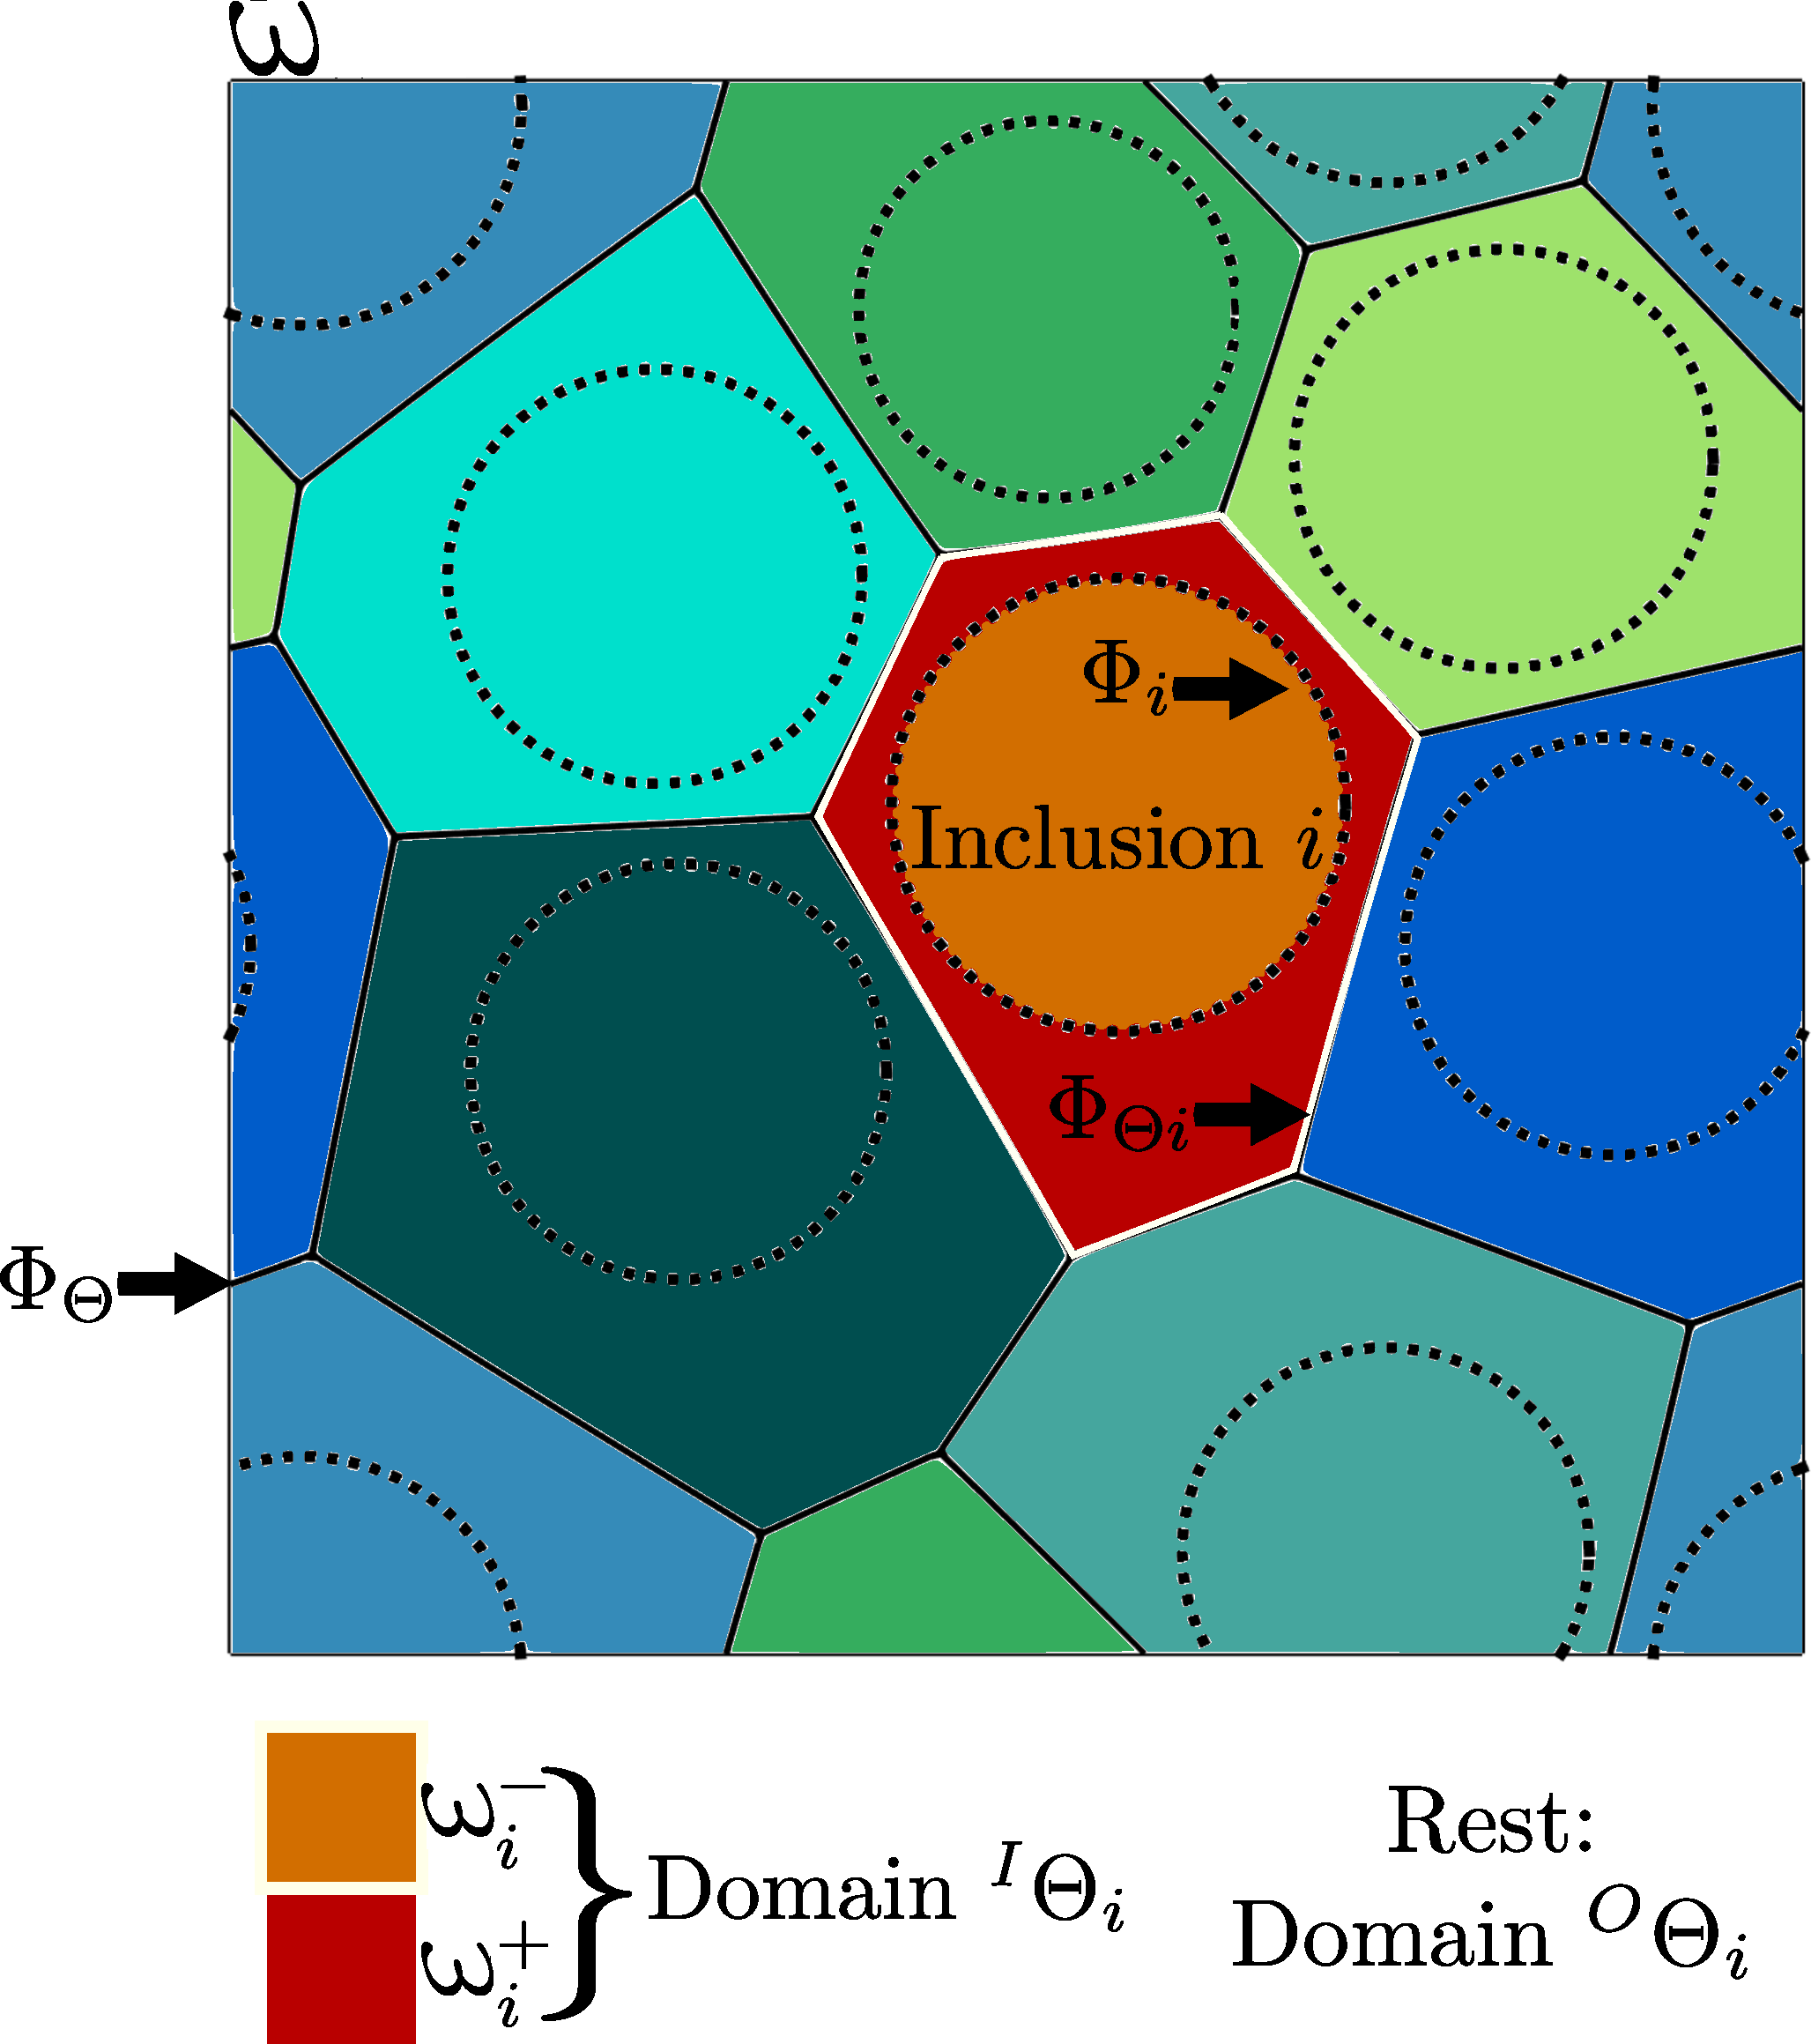
\includegraphics[height=7cm]{NNL_OMEGA}
	\caption{Domain definitions; Dashed lines denote inclusion boundaries while bold lines denote $ \Phi_\Theta$.}\label{omega}
\end{figure}

If we consider a domain $ \omega $ (Figure \ref{omega}), where we want to introduce an inclusion $ i  $, member of the set $ \textbf{I} $ of all inclusions, then $ \omega_i^- $ represents the domain inside the boundary of the inclusion denoted by $ \Phi_i $ and $ \omega_i^+ $ the domain outside $ \Phi_i $. $ DS_i(\textbf{x}) $ is defined as the signed distance field of $ i $, with negative value in $ \omega_i^- $ and positive value in $ \omega_i^+ $. At every position $ \textbf{x} $ \footnote{In this chapter, as compared to Chapter \ref{chap-ch}, the subscript ``m'' of $ \tgmm{x}\in\omega $ is omitted for conciseness.}, $ DN_k(\textbf{x}) $ gives the distance from $k $-th nearest $ \Phi_i $ in the packing and thus, all inclusions in the packing can be represented by using $ DN_1(\textbf{x}) $ as a level set. $ NN_k(\textbf{x}) $ denotes the $ k $-th neighbor identity map. As an integer discontinuous function, at each point in the domain, $ \textbf{x} $, it denotes the nearest inclusion from $ \textbf{x} $ in the set $ \textbf{I} $. $ \textbf{J}_k(\textbf{x}) $ defines an $ \textbf{x} $ dependent set constructed from $ \textbf{I} $ excluding all $ NN_m $, $ m\in[1:k-1] $. 
This quantity is computationally free and helps constructing $ DN_k(\textbf{x}) $ as:
\begin{equation}
DN_k(\textbf{x})=\displaystyle\min_j(DS_j(\textbf{x})),\text{with $ j $ in } \textbf{J}_k(\textbf{x}).
\end{equation}
We further define $ ^I\Theta_i $ as the ``Inner" domain where inclusion $ i $ is the first nearest inclusion. It is the set of points $ \textbf{x} $  closer to inclusion $ i $ than to any other inclusion, i.e. where $ NN_1(\textbf{x})=i, \forall\, \textbf{x} \in {^I\Theta_i} $. Similarly, $ ^O\Theta_i $ is the ``Outer" domain where $ NN_1(\textbf{x})\ne i $. $ \Phi_{\Theta i} $ is the boundary of $ ^I\Theta_i $ and $ \Phi_{\Theta} $ is the union of all $ \Phi_{\Theta i} $.

In RSA, the rejection rate of an inclusion is reduced with an \textit{a priori} knowledge of sub domains where the position of the inclusion will respect all the criteria of a positioning  test. Logical operations on the $ DN_k $ functions can help in selecting a large range of discrete structured or unstructured positions in the RVE discretizing the description of the neighboring distance functions. For arbitrary shaped inclusions, the smallest enclosing circle/sphere (SEC / SES) of radius $ r $ determines the non-overlap criteria on any inclusion in the RVE already mapped in $ DN_1(\textbf{x}) $ when the condition  
\begin{equation}
 DN_1(\textbf{x}_c)>r \label{secses1}
\end{equation}
is satisfied for its center $ \textbf{x}_c $. In the case of circular/spherical inclusions, $r$, $  \forall r \in \mathbb{R} $, is a realization of the random variable $ \textit{X} $ such that $X\sim\textbf{Pr}(p)$, $\textbf{Pr}(p)$ being a radius distribution (like normal, log-normal or gamma distributions) and where the sign $ \sim $ means that the random variable follows the chosen distribution.

\begin{figure}
	\centering
	\begin{subfigure}[t]{0.3375\textwidth}
		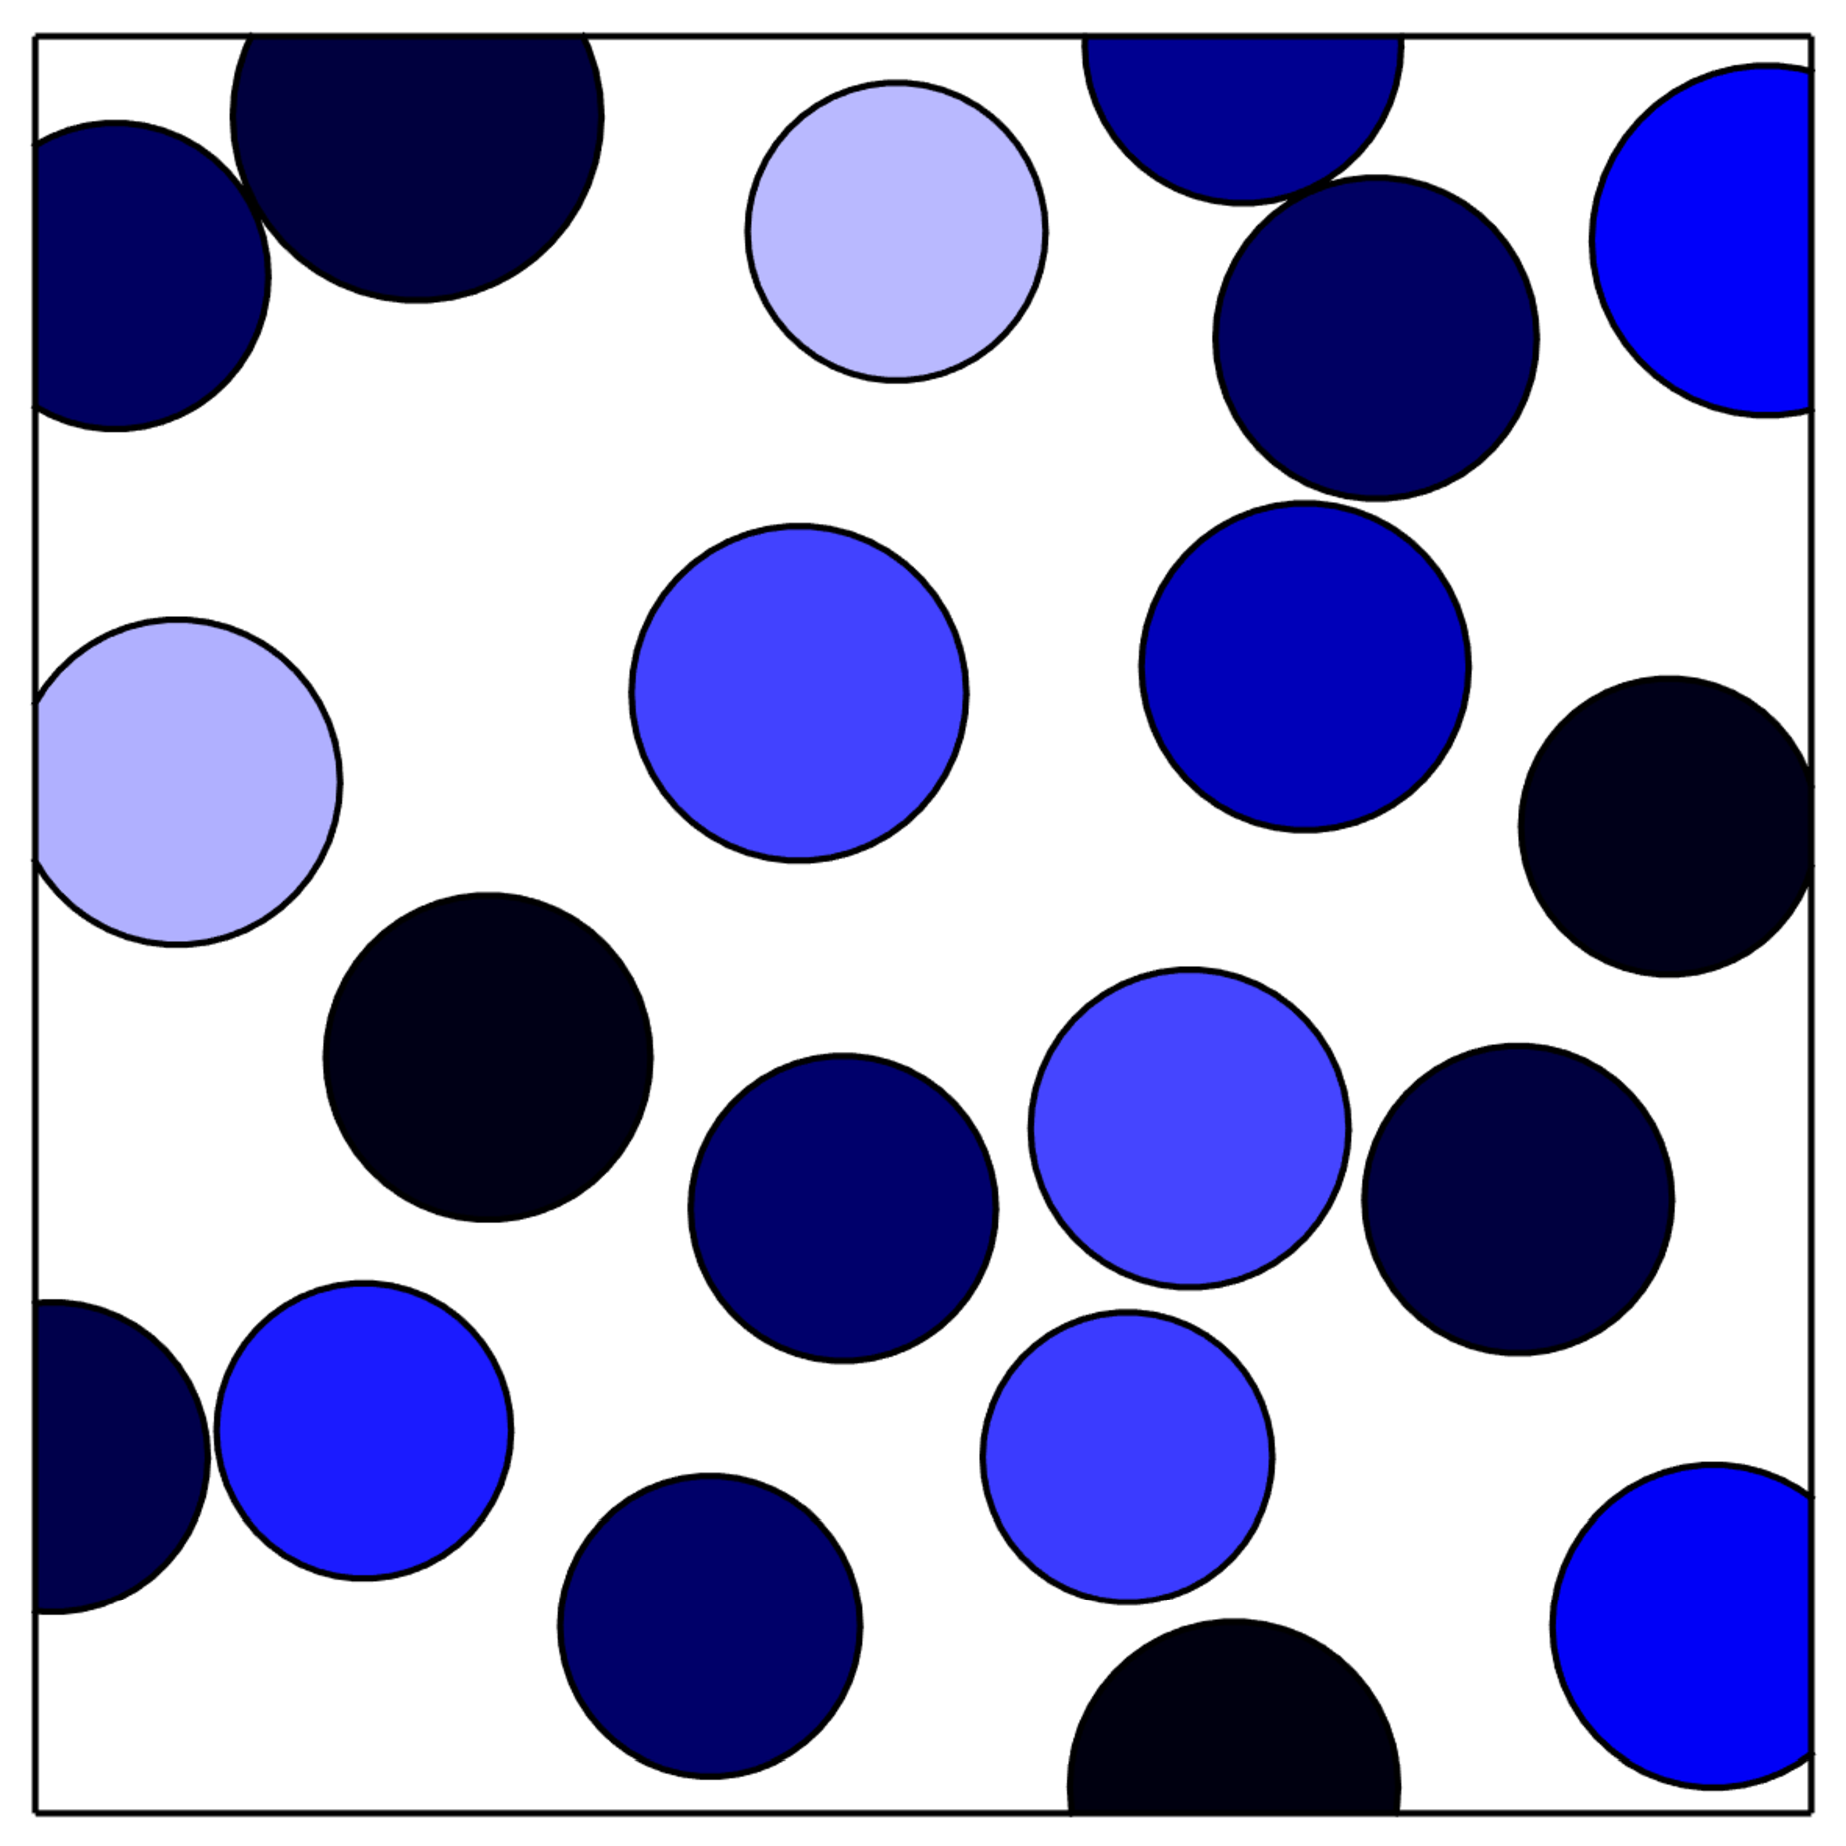
\includegraphics[width=\textwidth]{NNL_RSA}	
		\caption{}
	\end{subfigure}
	\begin{subfigure}[t]{0.3375\textwidth}
		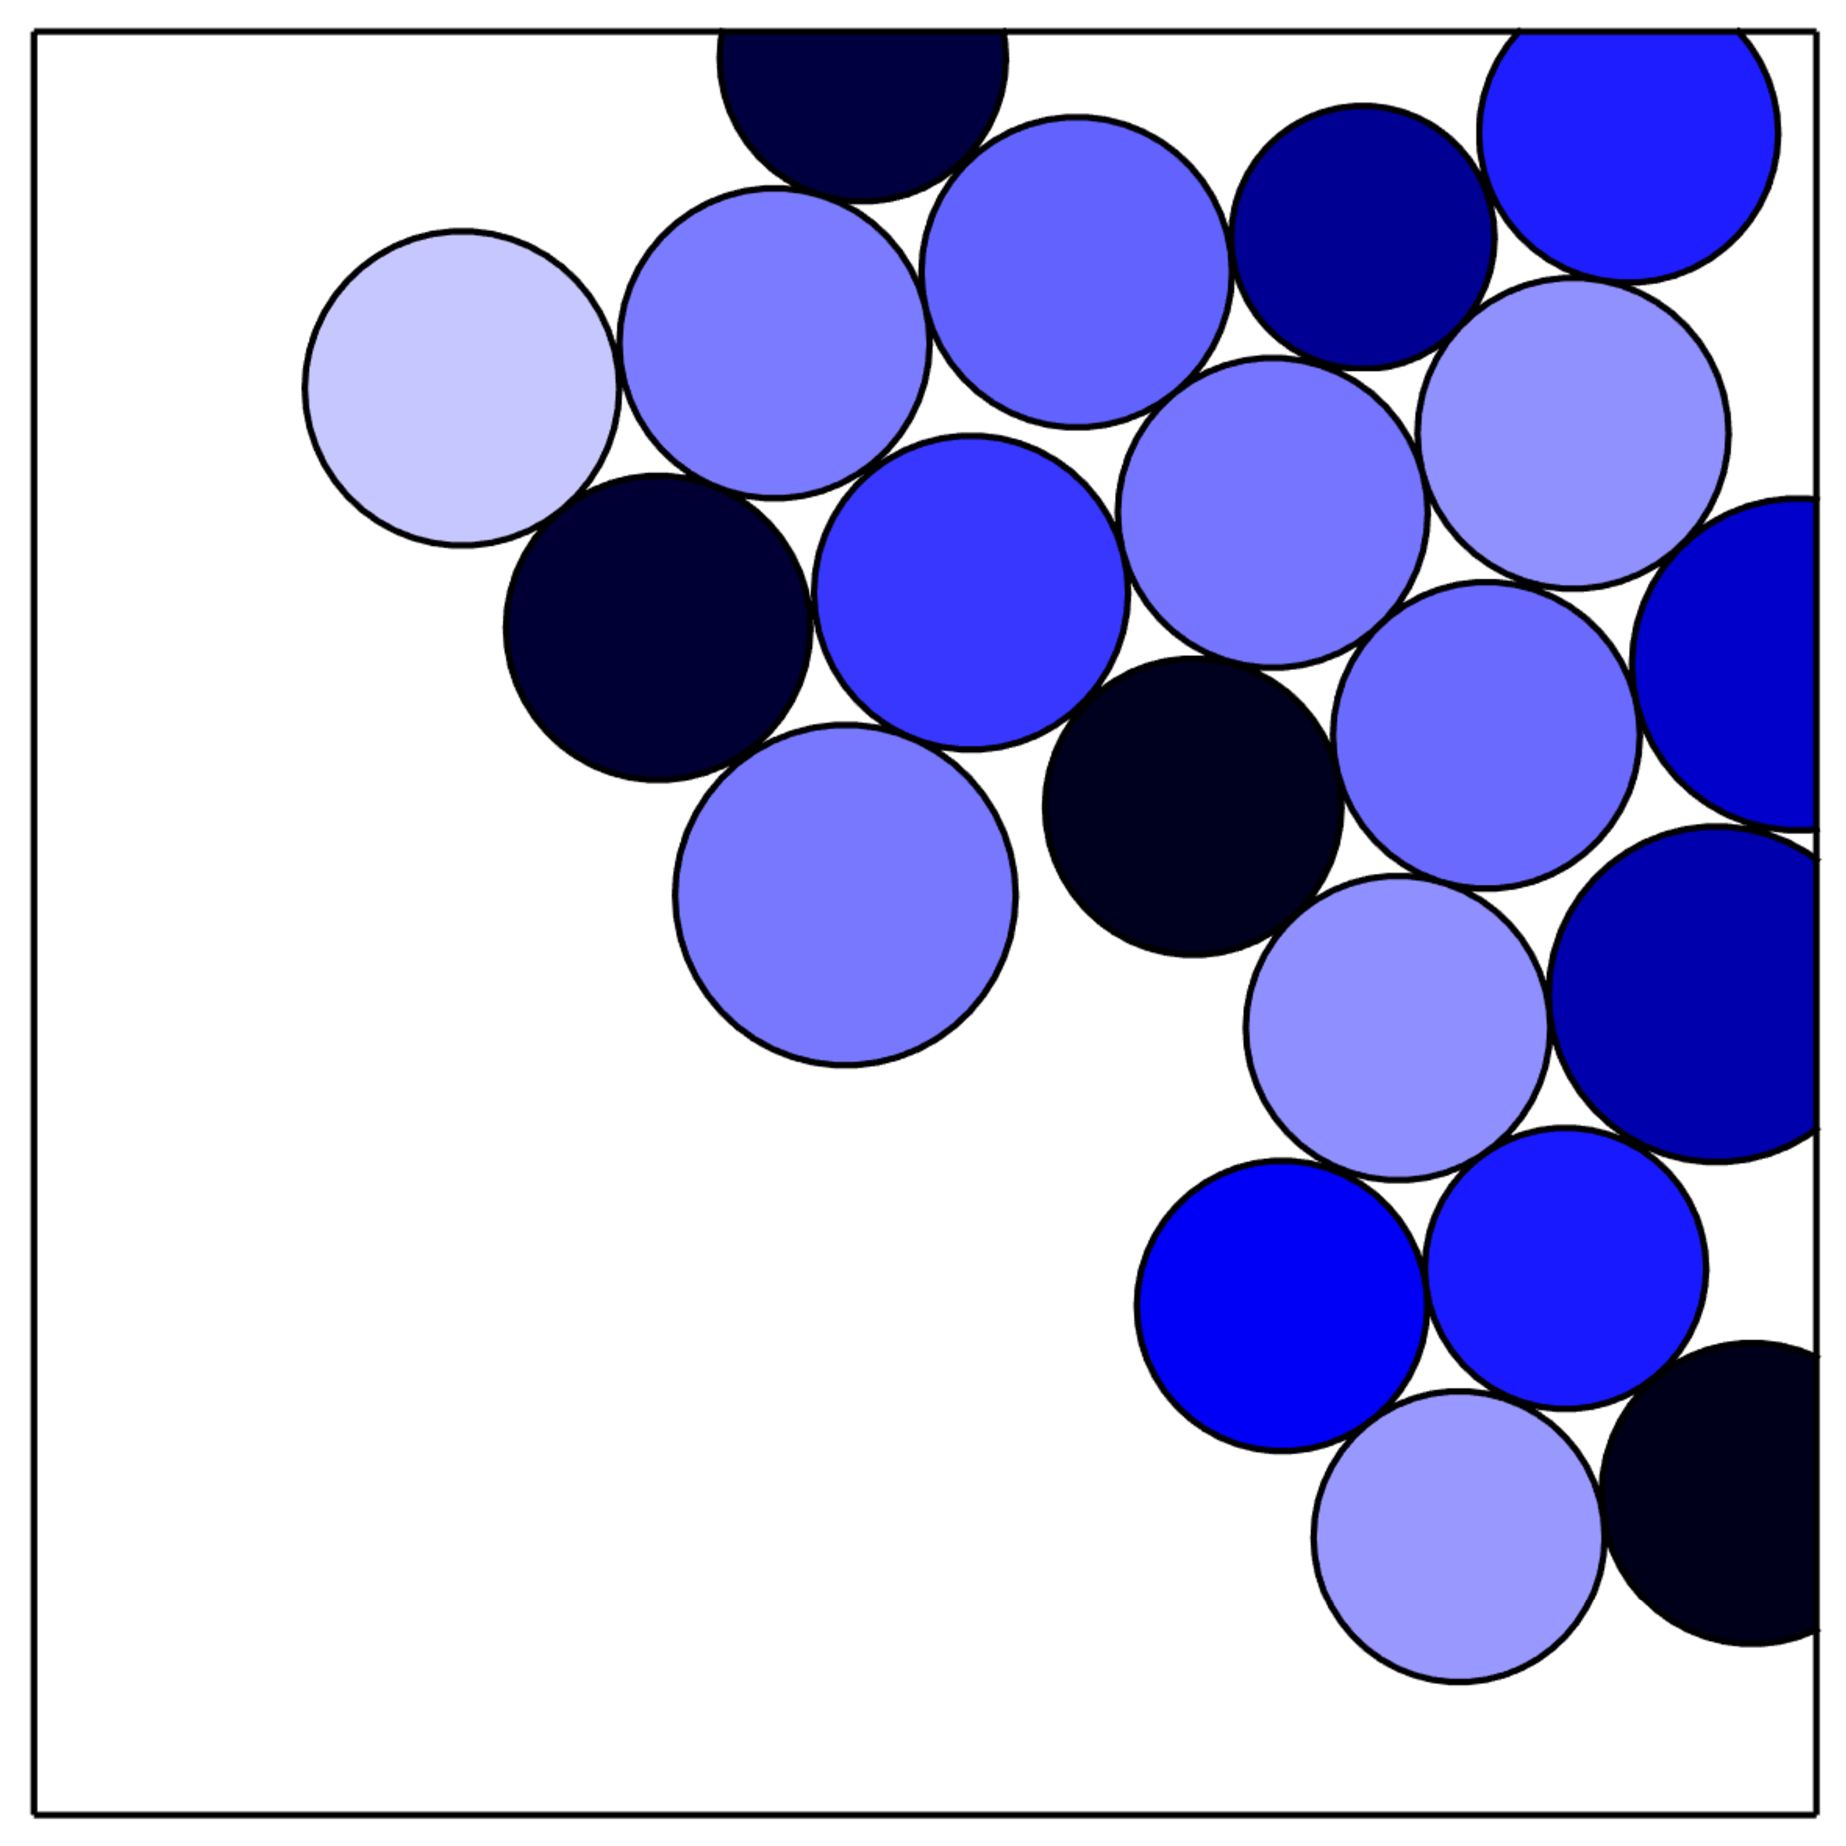
\includegraphics[width=\textwidth]{NNL_OPT}	
		\caption{}
	\end{subfigure}
	\caption{Effect of $nnl$ on the packing of an RVE with 20 inclusions; (a) Non-overlap control only, and (b) enforcing a minimal neighboring distance.}\label{nnl}
\end{figure}

A control on the distances from the first and the second nearest neighbors in 2D, and the third nearest neighbor in 3D (denoted by $ nnl_1 $, $ nnl_2 $ and $ nnl_3 $ in the sequel) can help in producing closer packings, thus enabling higher packing densities (Figure \ref{nnl}). Taking inspiration from algorithms like the clustering approach \cite{kimEffectRearrangementSimulated2002} and the advancing front \cite{bagiAlgorithmGenerateRandom2005}, where the inclusions are placed on the vertices of triangles (2D) or tetrahedra (3D) to position the new inclusion  close to the existing two or three nearest neighbors, the condition
\begin{equation}
DN_k(\textbf{x}_c)<nnl_k+r\label{secses2}
\end{equation} is introduced, where\[ k = \begin{cases}
\{1;2\} \text{ in 2D};
\\\{1;2;3\}\text{ in 3D}.
\end{cases} \]
Higher $ k $ values can also be considered which can then be used for various operations on the morphologies, such as the one described in Section \ref{sec-concavity}.

\begin{figure}
	\centering
	\begin{subfigure}[t]{0.37\textwidth}
		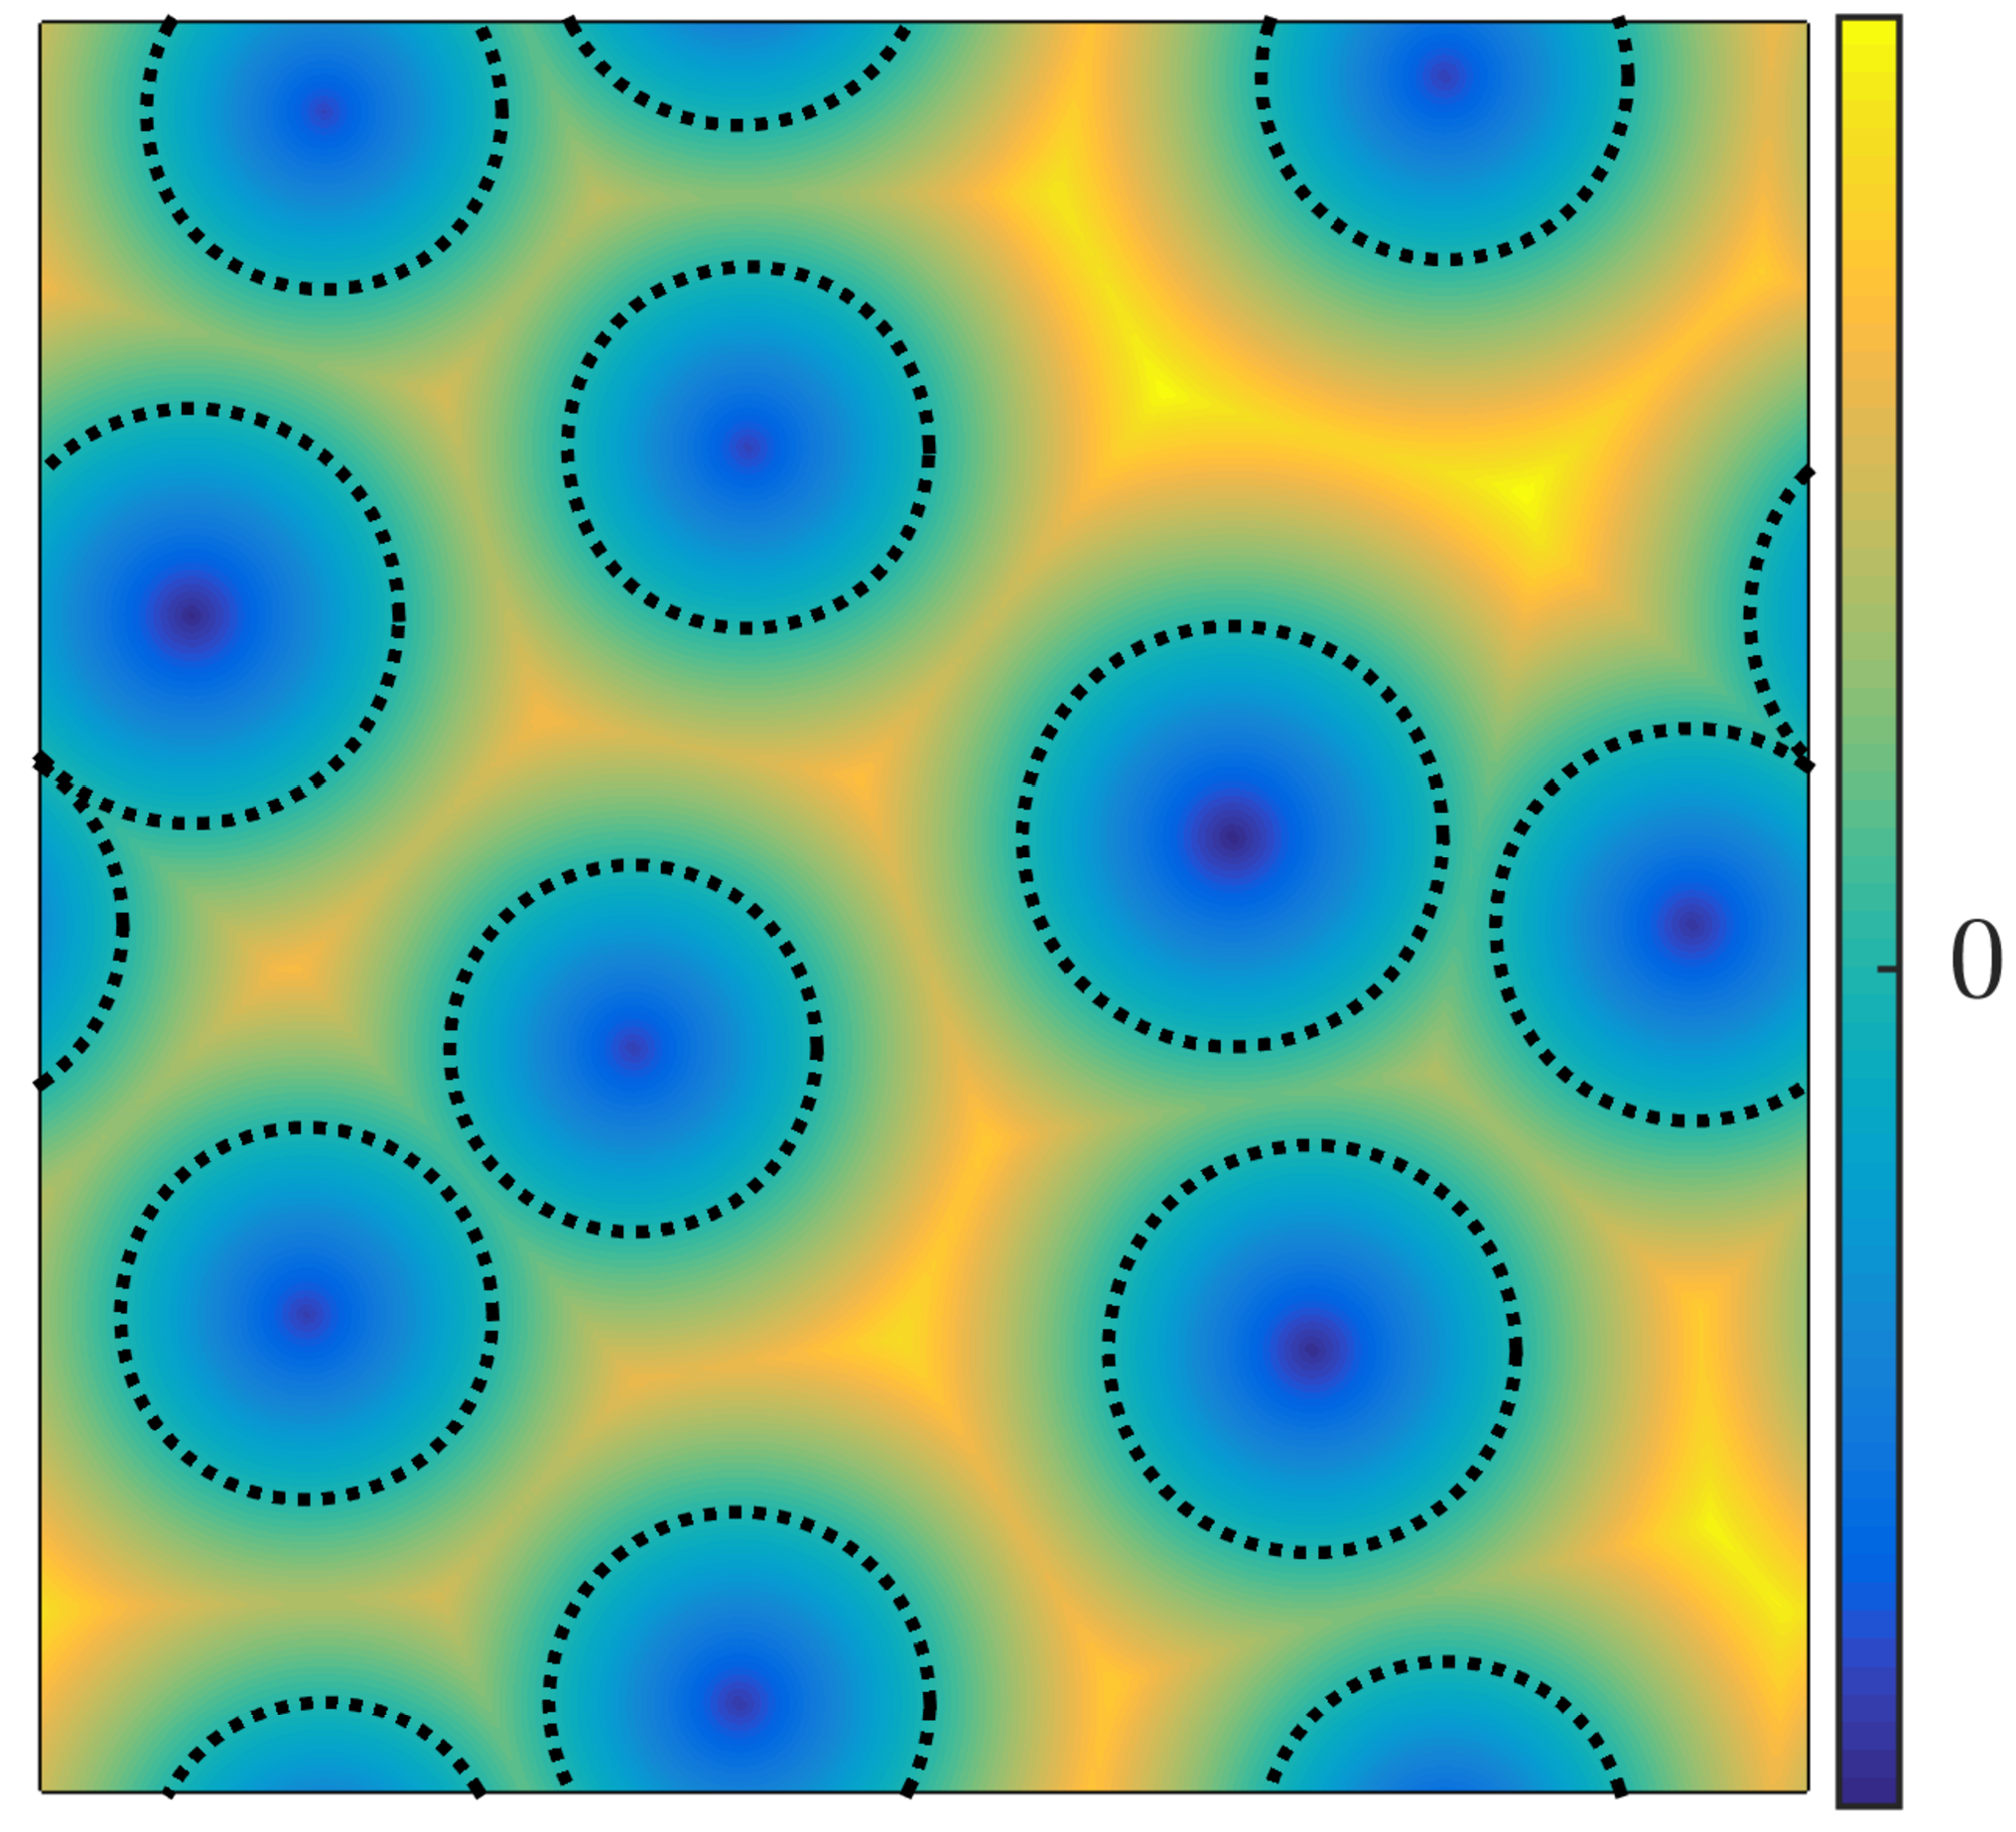
\includegraphics[width=\textwidth]{NNL_LS1}	
		\caption{}
	\end{subfigure}
	\begin{subfigure}[t]{0.33\textwidth}
		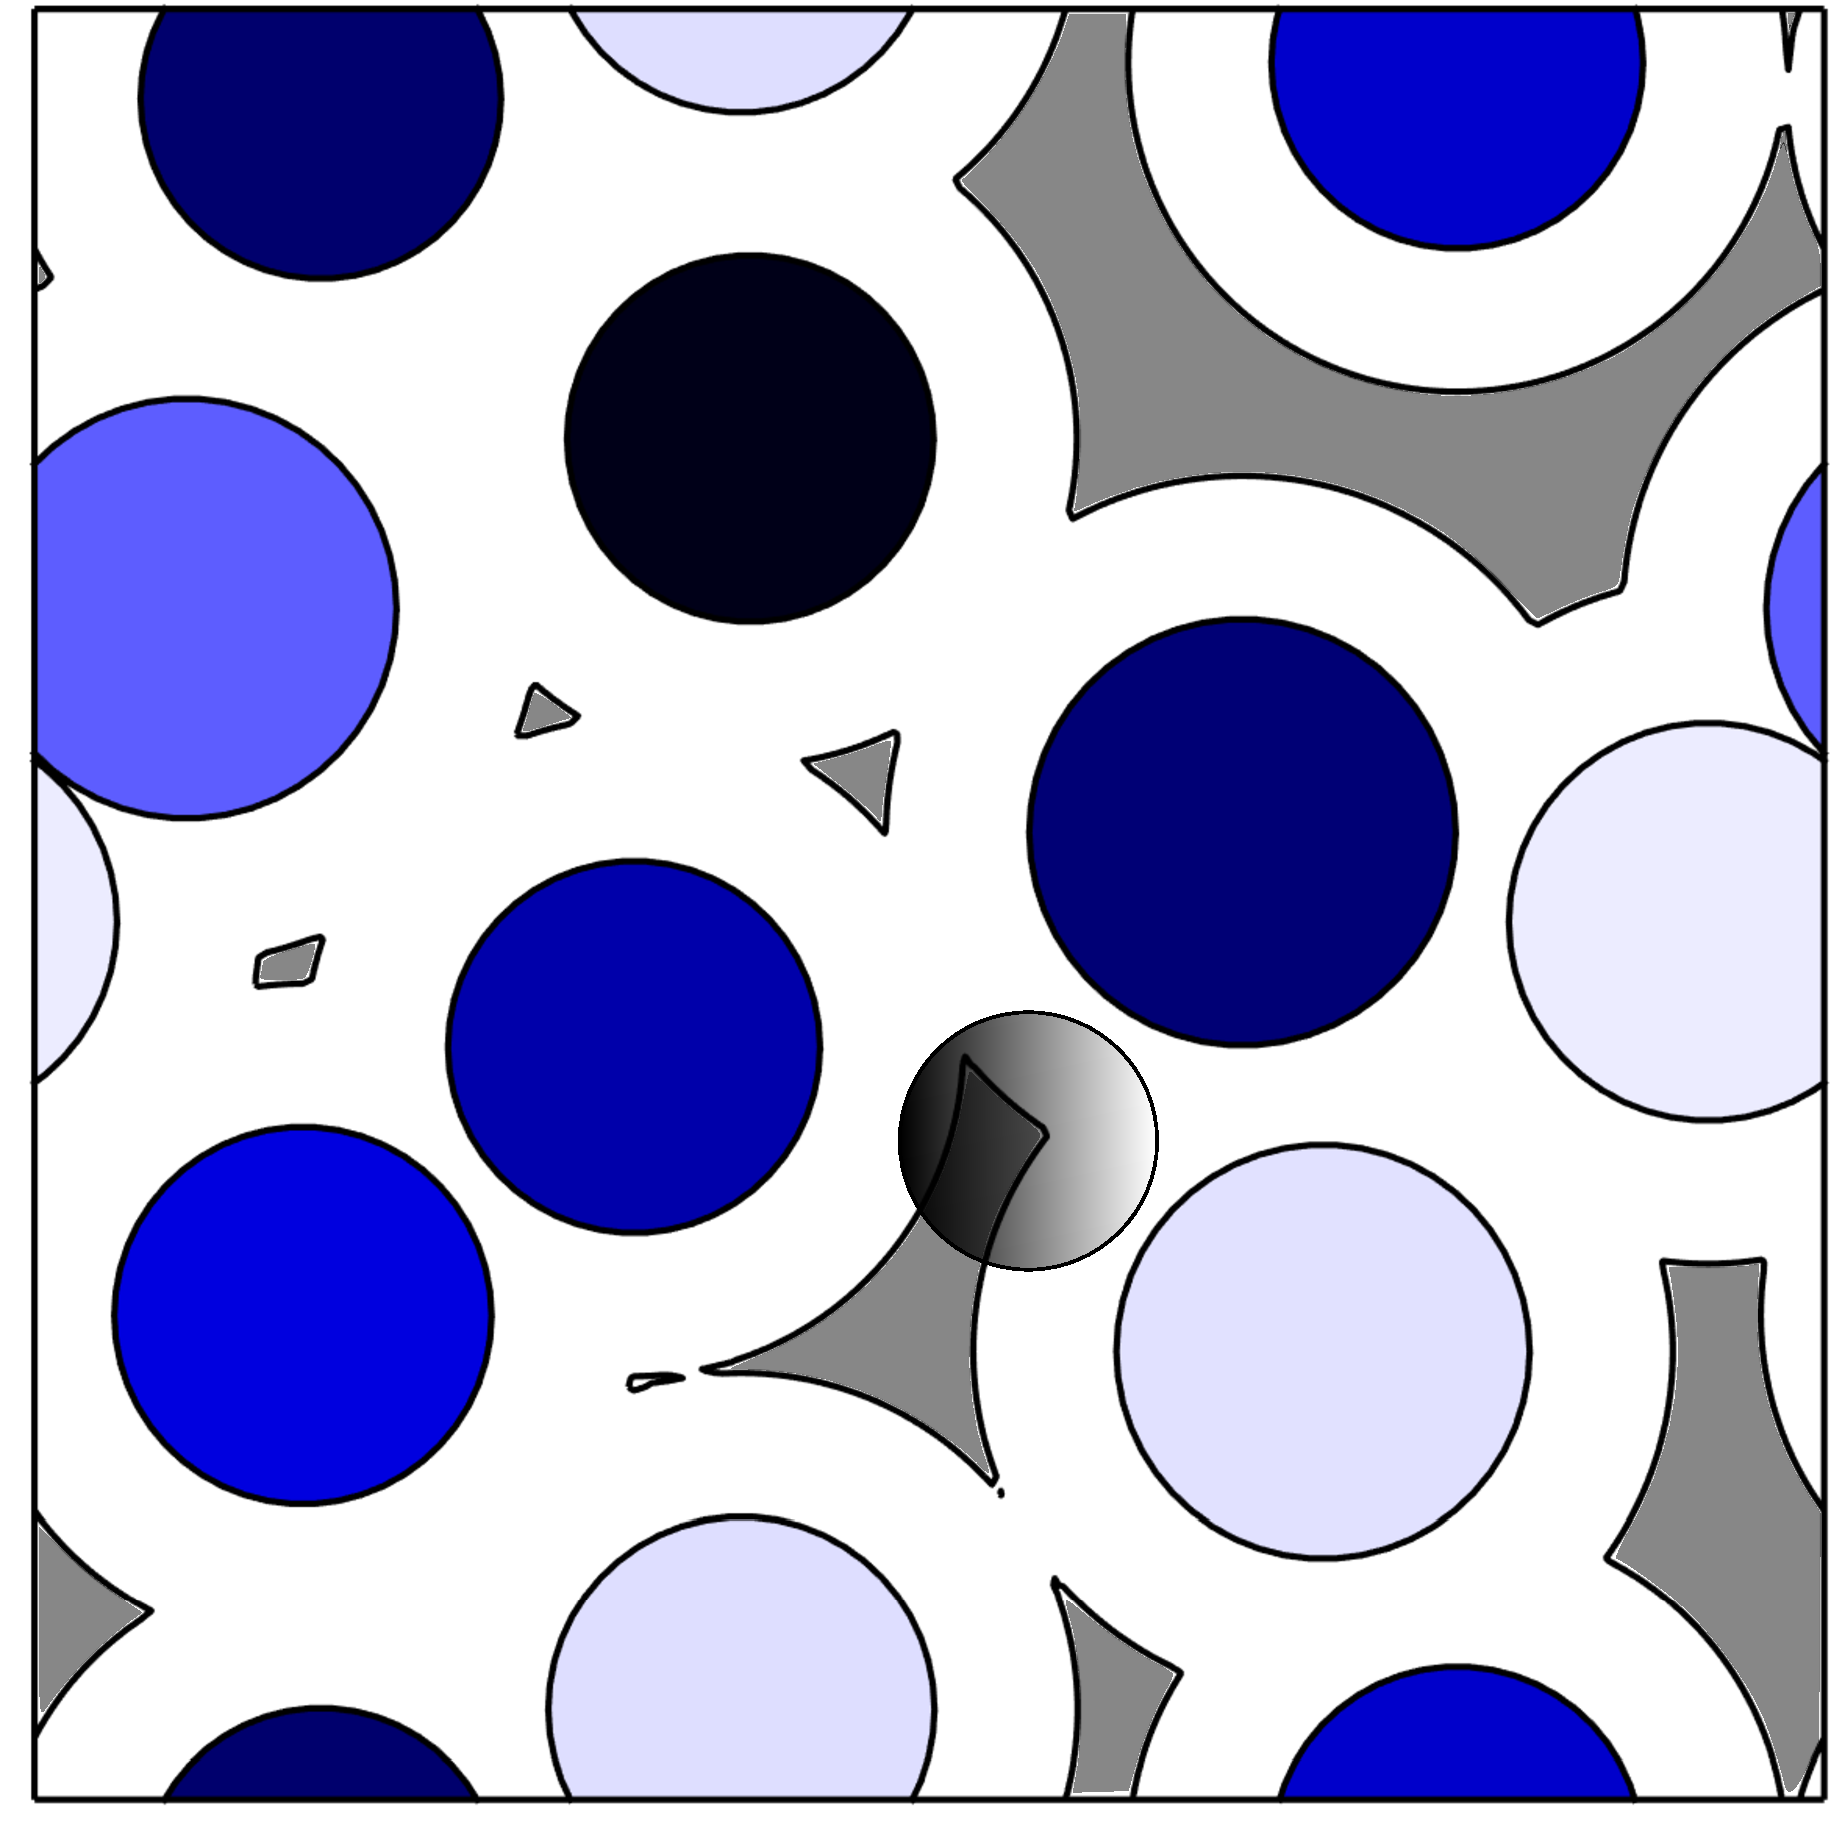
\includegraphics[width=\textwidth]{NNL}	
		\caption{}
	\end{subfigure}
	\caption{(a) $DN_1$ function plot. (b) Using Eqs. (\ref{secses1}) or (\ref{secses2}) the shaded domain can be extracted where the criteria for the next inclusion is satisfied. }\label{rsa_rsa}
\end{figure}

Thus, the DN-RSA can be summarized as follows:
\begin{enumerate}
	\item Construct a discretized RVE domain made of a regular grid of points $ \textbf{x}_n $ and initialize $ DN_k(\textbf{x}_n) $ to $ +\infty $.
	\item Generate a trial inclusion $ i $ from the prescribed size distribution function / predefined set.
	\item Use condition (\ref{secses1}) to avoid inter-penetration and condition (\ref{secses2}) to  meet neighbor distance criteria, retaining all satisfactory $ \textbf{x}_c $ (Figure \ref{rsa_rsa}). If this is empty, the RVE is full for the inclusion size considered, thus terminating the process.
	\item Refresh $ DN_k(\textbf{x}_n) $ to allow the calculation of $ DS_i(\textbf{x}_n) $ of a new inclusion $ i $ using a sequential adaptive refreshing.
	\item Follow step 2 until the termination criterion is reached or the RVE is full (Figure \ref{dn-rsa}).
\end{enumerate}
\begin{figure}
	\centering
	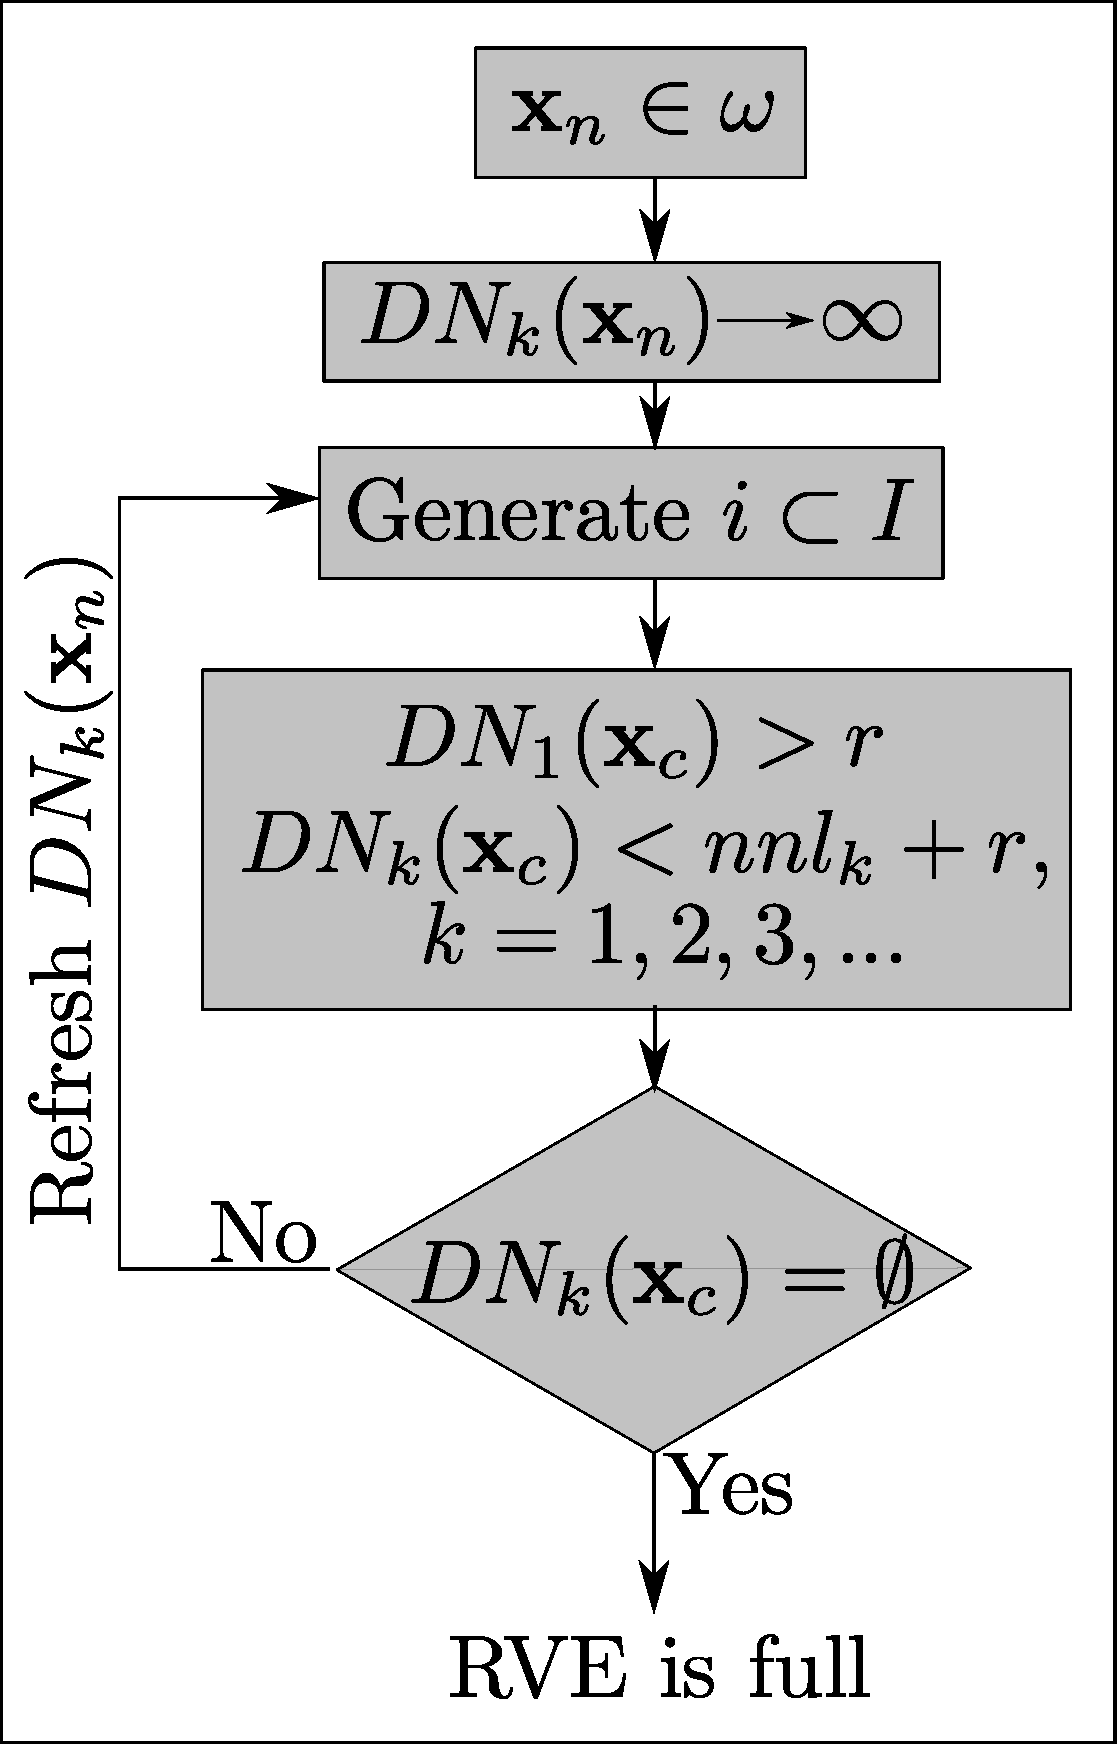
\includegraphics[width=4cm]{flowchart1}
	\caption{DN-RSA process.}\label{dn-rsa}
\end{figure}
To increase the computational efficiency of the $ DN_k $ evaluations, a sequential adaptive scheme is introduced. {In such a scheme the contribution of each $ DS_i $ is introduced simultaneously in functions $ DN_k $ as inclusions are introduced sequentially along time represented by an index $ m $}, using:
\begin{equation}
DN_1(\textbf{x})^m=\min(DN_1(\textbf{x})^{m-1},DS_i(\textbf{x})^m),
\end{equation}
\begin{equation}
\begin{split}
DN_k(\textbf{x})^m=&\max\left(DN_{k-1}(\textbf{x})^{m-1},\,\min(DN_k(\textbf{x})^{m-1},DS_i(\textbf{x})^m)\right).
\end{split}
\end{equation}
The differences in the first three $ DN_k $ functions have been illustrated in Figure \ref{dn1}\footnote{In all illustrations provided in this chapter, RVEs are considered with unit lengths in all directions. The scale reported with the $ DN_k $ functions in Figure \ref{dn1} should therefore be understood in relative terms with respect to the RVE dimensions.}.

\begin{figure}
	\centering

	\begin{subfigure}[t]{0.32\textwidth}
	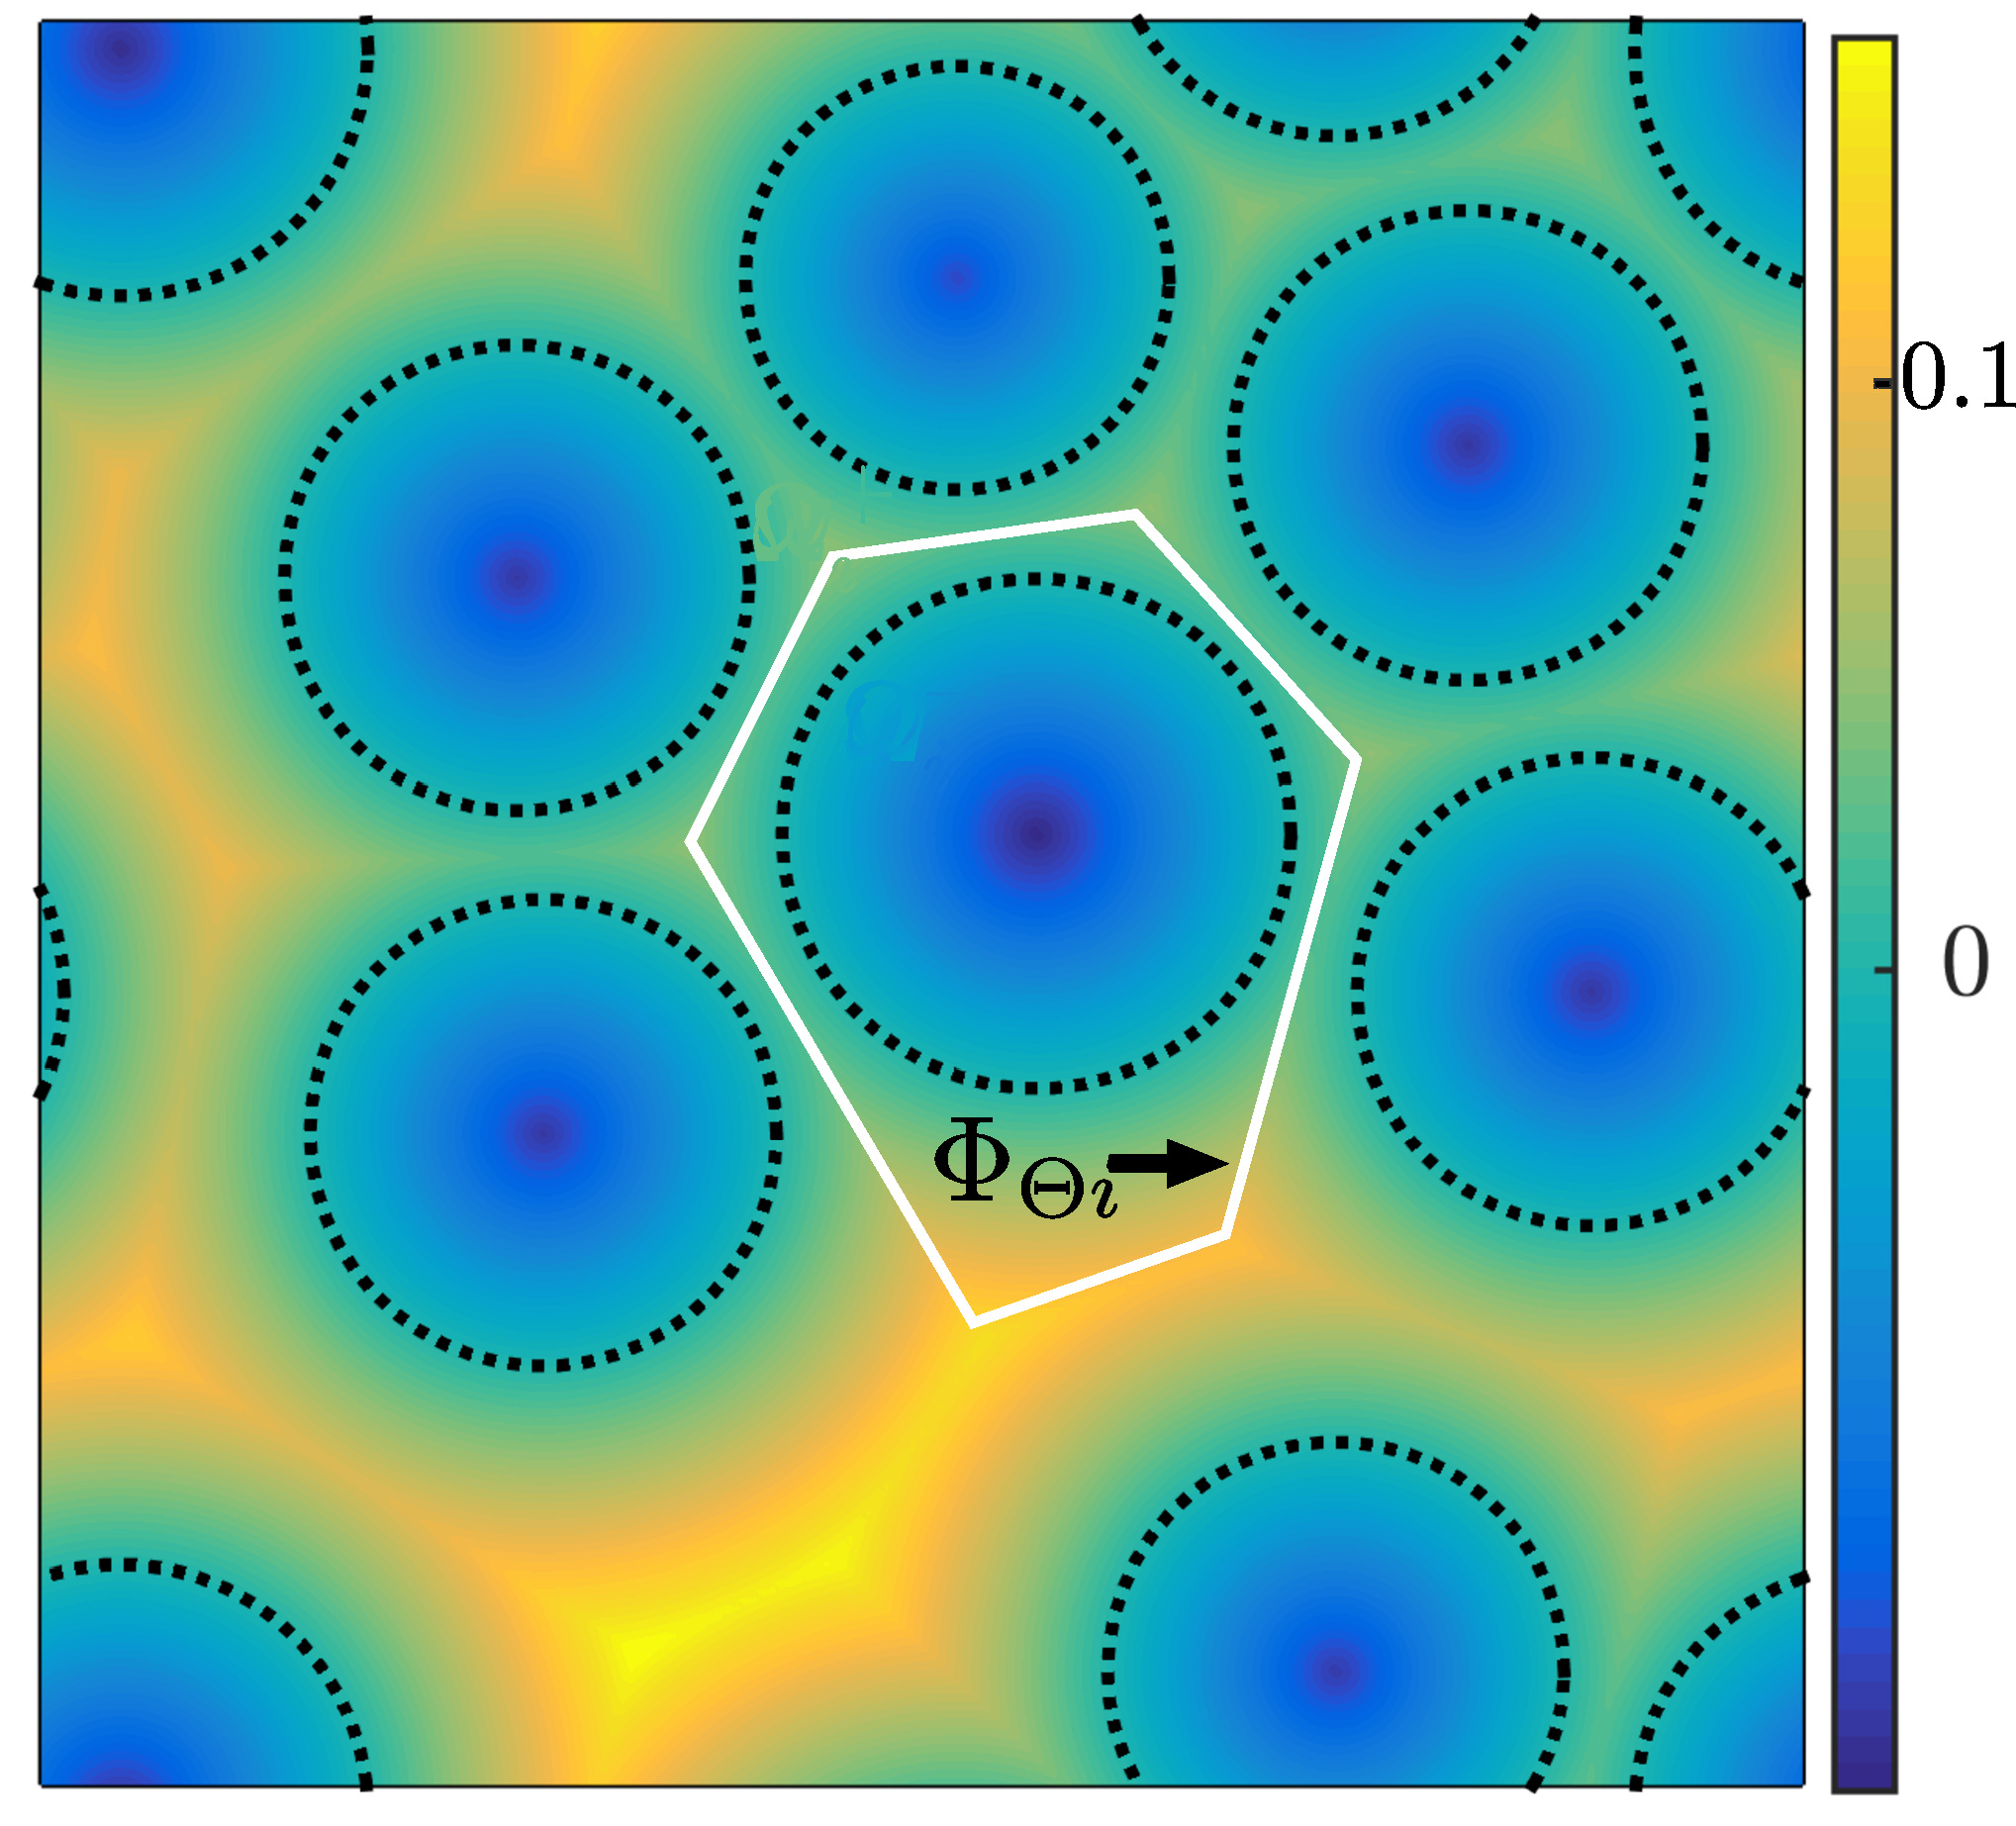
\includegraphics[width=\textwidth]{LS1}	
	\caption{}
	\end{subfigure}
	\begin{subfigure}[t]{0.32\textwidth}
	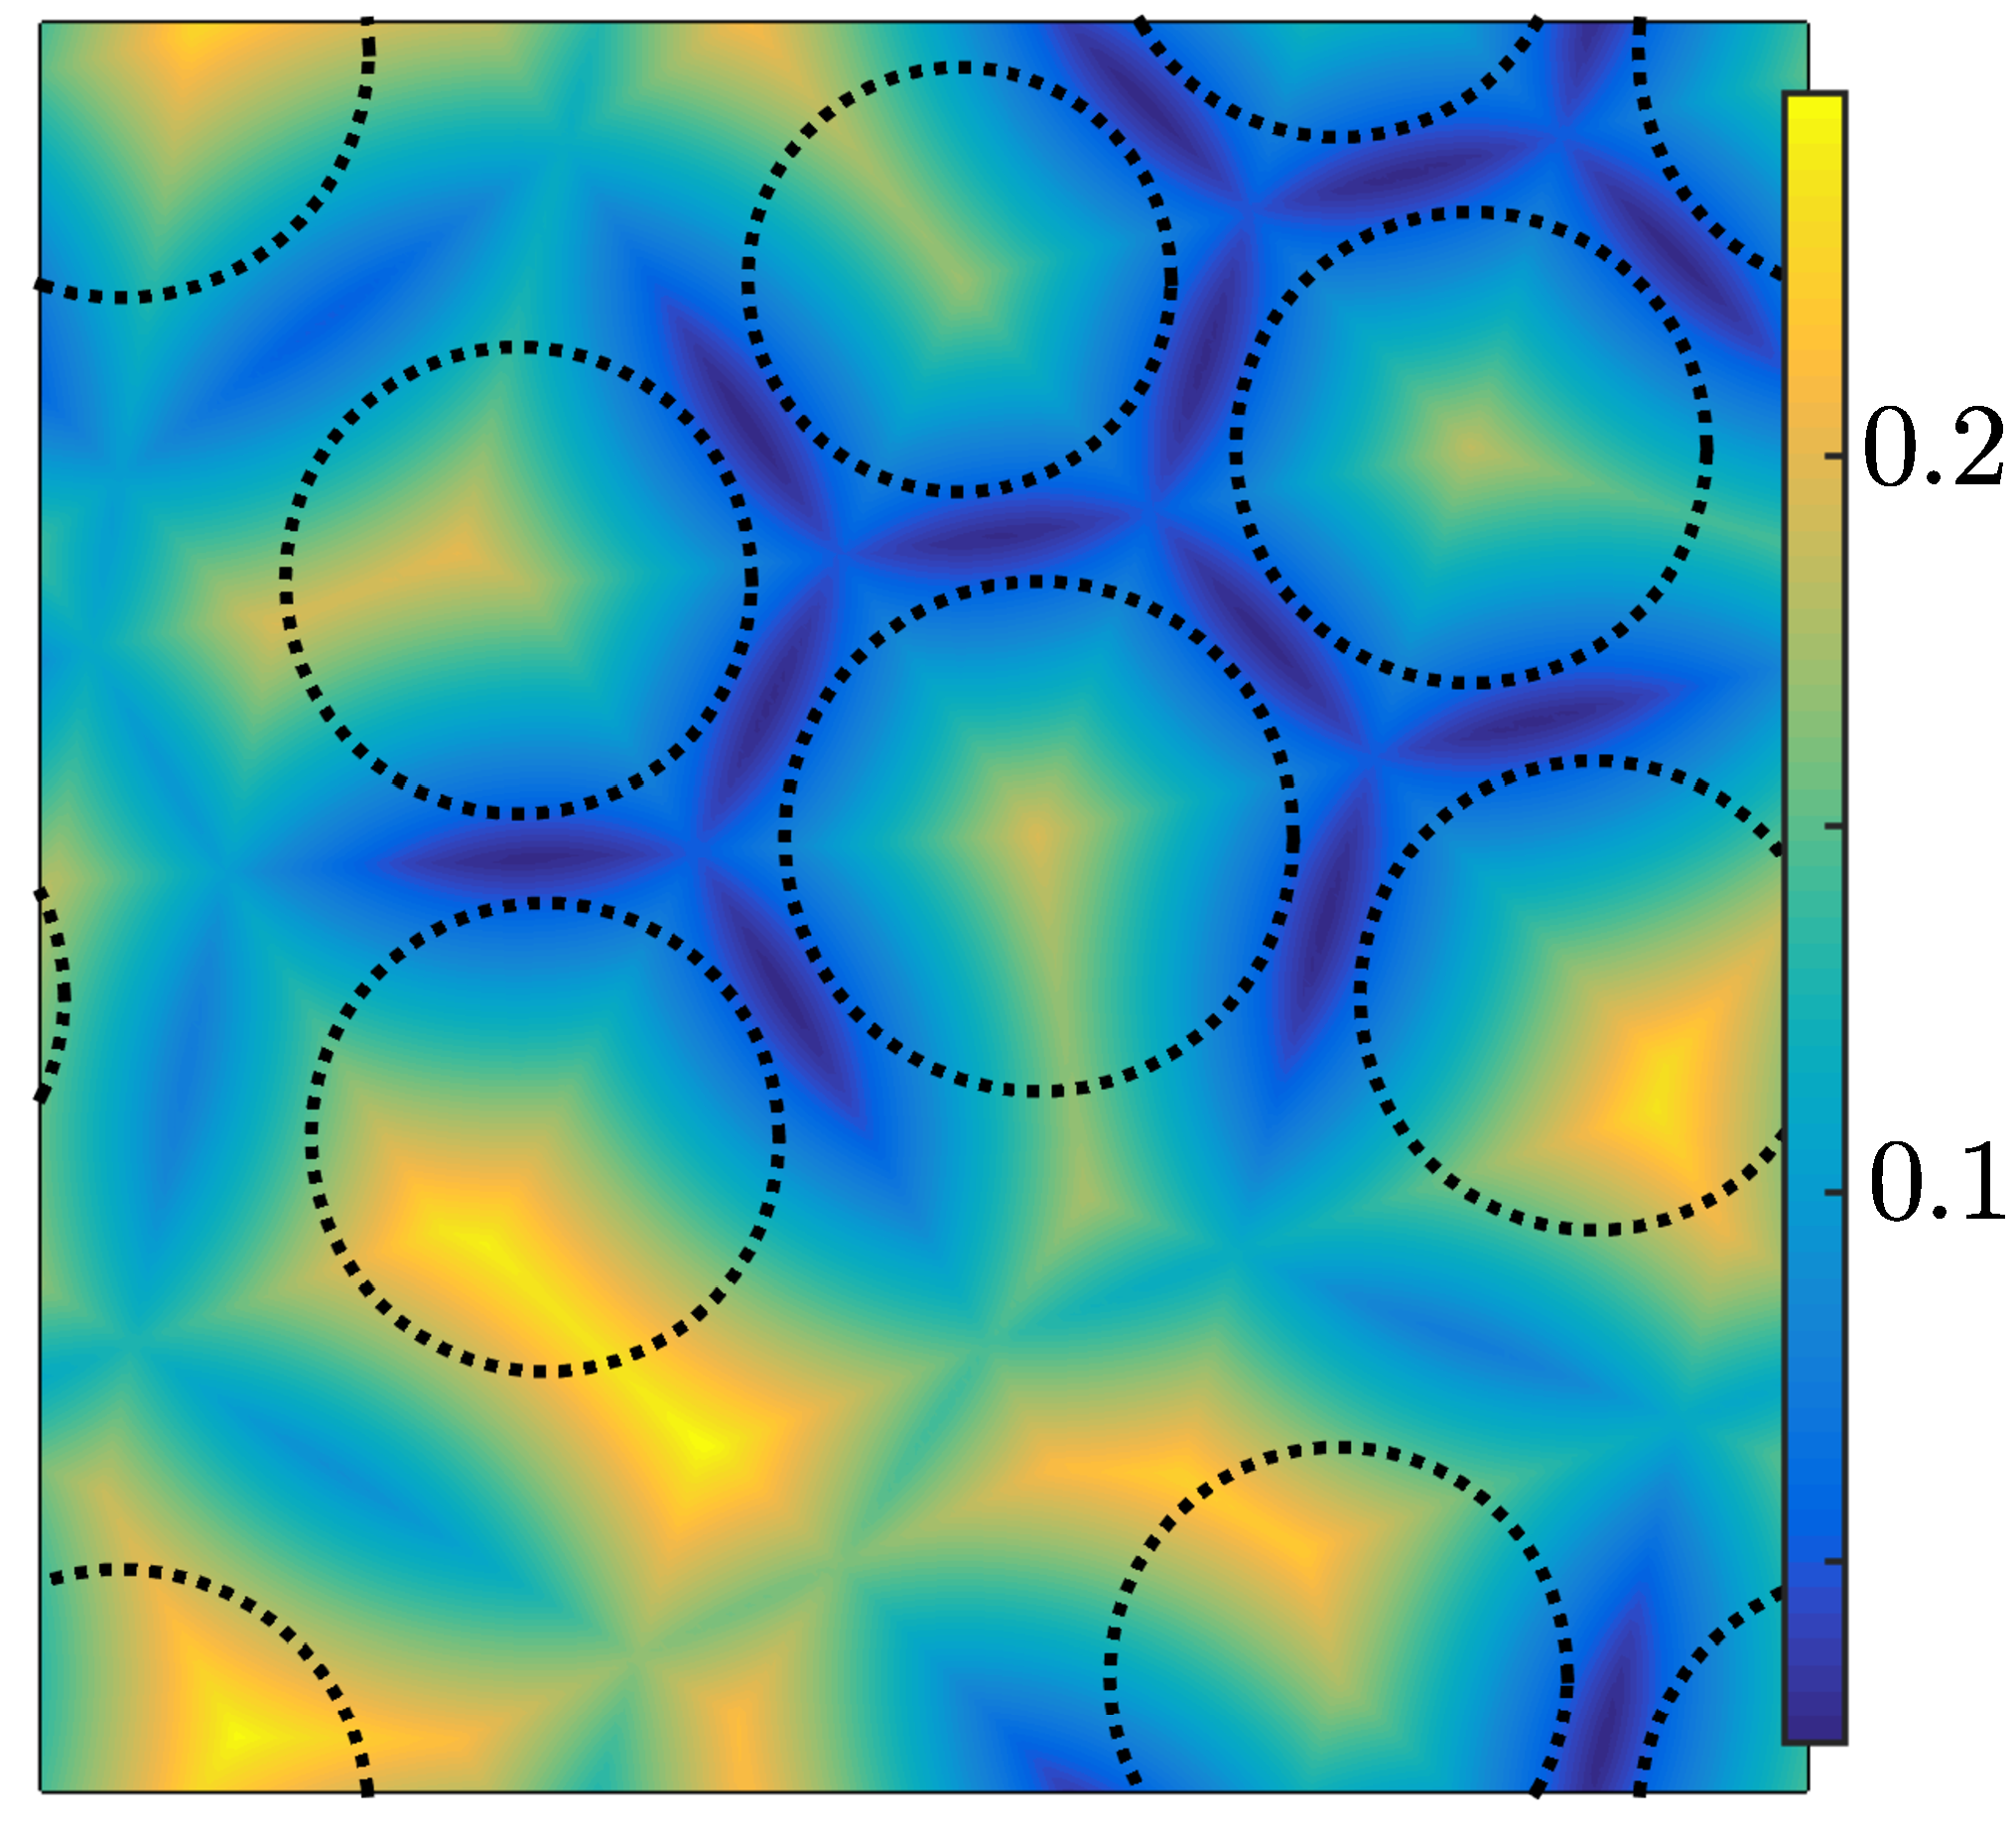
\includegraphics[width=\textwidth]{LS2}	\label{dn2}
	\caption{}
	\end{subfigure}
	\begin{subfigure}[t]{0.32\textwidth}
	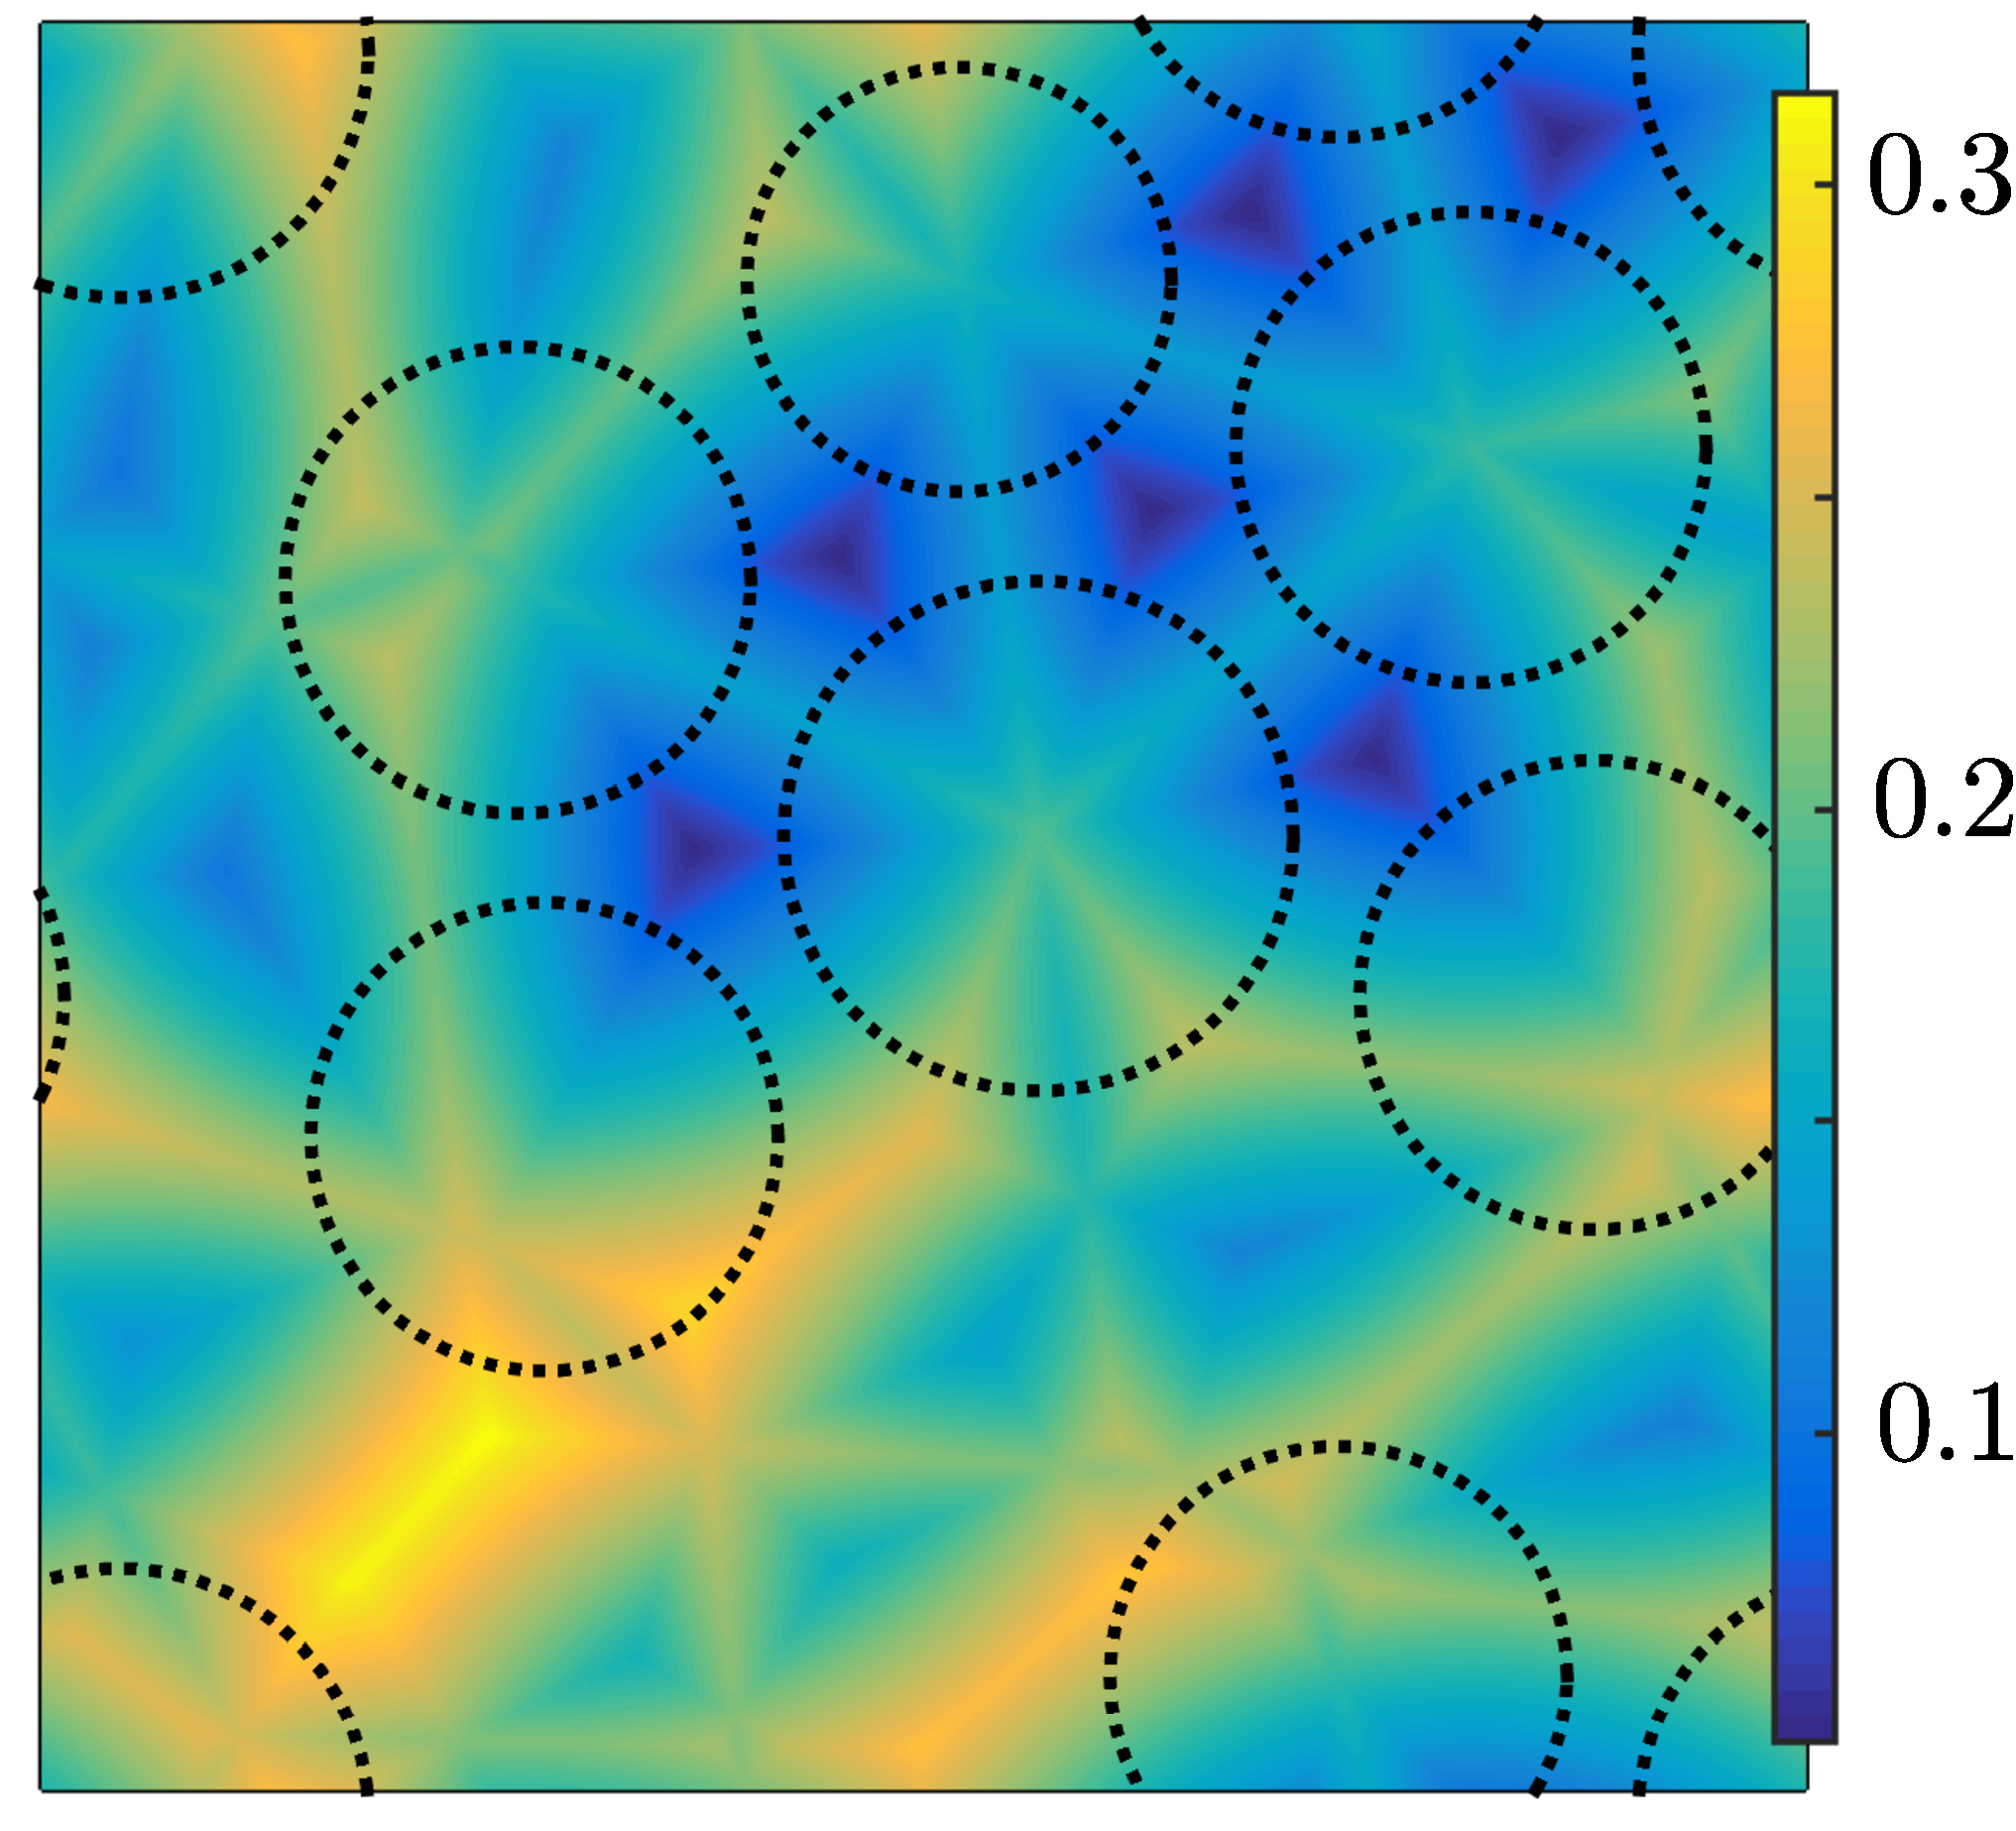
\includegraphics[width=\textwidth]{LS3}	\label{dn3}
	\caption{}
	\end{subfigure}
	\caption{Functions (a) $DN_1$, (b) $DN_2$, and (c) $DN_3$. $ \Phi_{\Theta i}$ is marked for comparison.}\label{dn1}
\end{figure}

Application of periodicity in the RVE boundaries may be advantageous in obtaining statistically homogeneous RVEs without border effects that introduce morphological difference between the bulk of the RVE and its boundary neighborhood. Also, homogenization techniques were shown to give better result while using periodic boundary conditions in the physical model \cite{hollisterComparisonHomogenizationStandard1992}(Figure \ref{periodic}). Nevertheless, free boundary conditions in RVE geometries enable generating models free of constraints induced by the periodicity of the RVE. In this case, to avoid the spatial sampling bias introduced due to the interaction of the inclusions at the boundary with the domain $ \omega $, minus sampling operation\label{text-minus} \cite{baddeleySpatialSamplingCensoring1999} can be considered where one samples only those objects that lie within a sampling frame (Figure \ref{free}). A maximum permissible unit length, which is smaller than the RVE dimensions, can be used such that the centers of all the objects the $\Phi_{\Theta i} $ of which are completely inside the domain lie inside this limit length. This quantity can be defined as a certain fraction of the dimensions of the RVE depending on the average size of the inclusions. More details on considerations related to the evaluation of periodic $ DN_k $ functions can be found in \cite{sononAdvancedTechniquesGeneration2014}.  It can be noted that the application of periodic boundary conditions on systems made of nonconformal or free boundary geometry can be solved by using specialized methods for this purpose \cite{nguyenComputationalHomogenizationCellular2014}. The methodology to extract open foam morphologies from the inclusion packings discussed in \cite{sononAdvancedApproachGeneration2015} is recalled next.

\begin{figure}
	\centering
	\begin{subfigure}[b]{0.32\textwidth}
		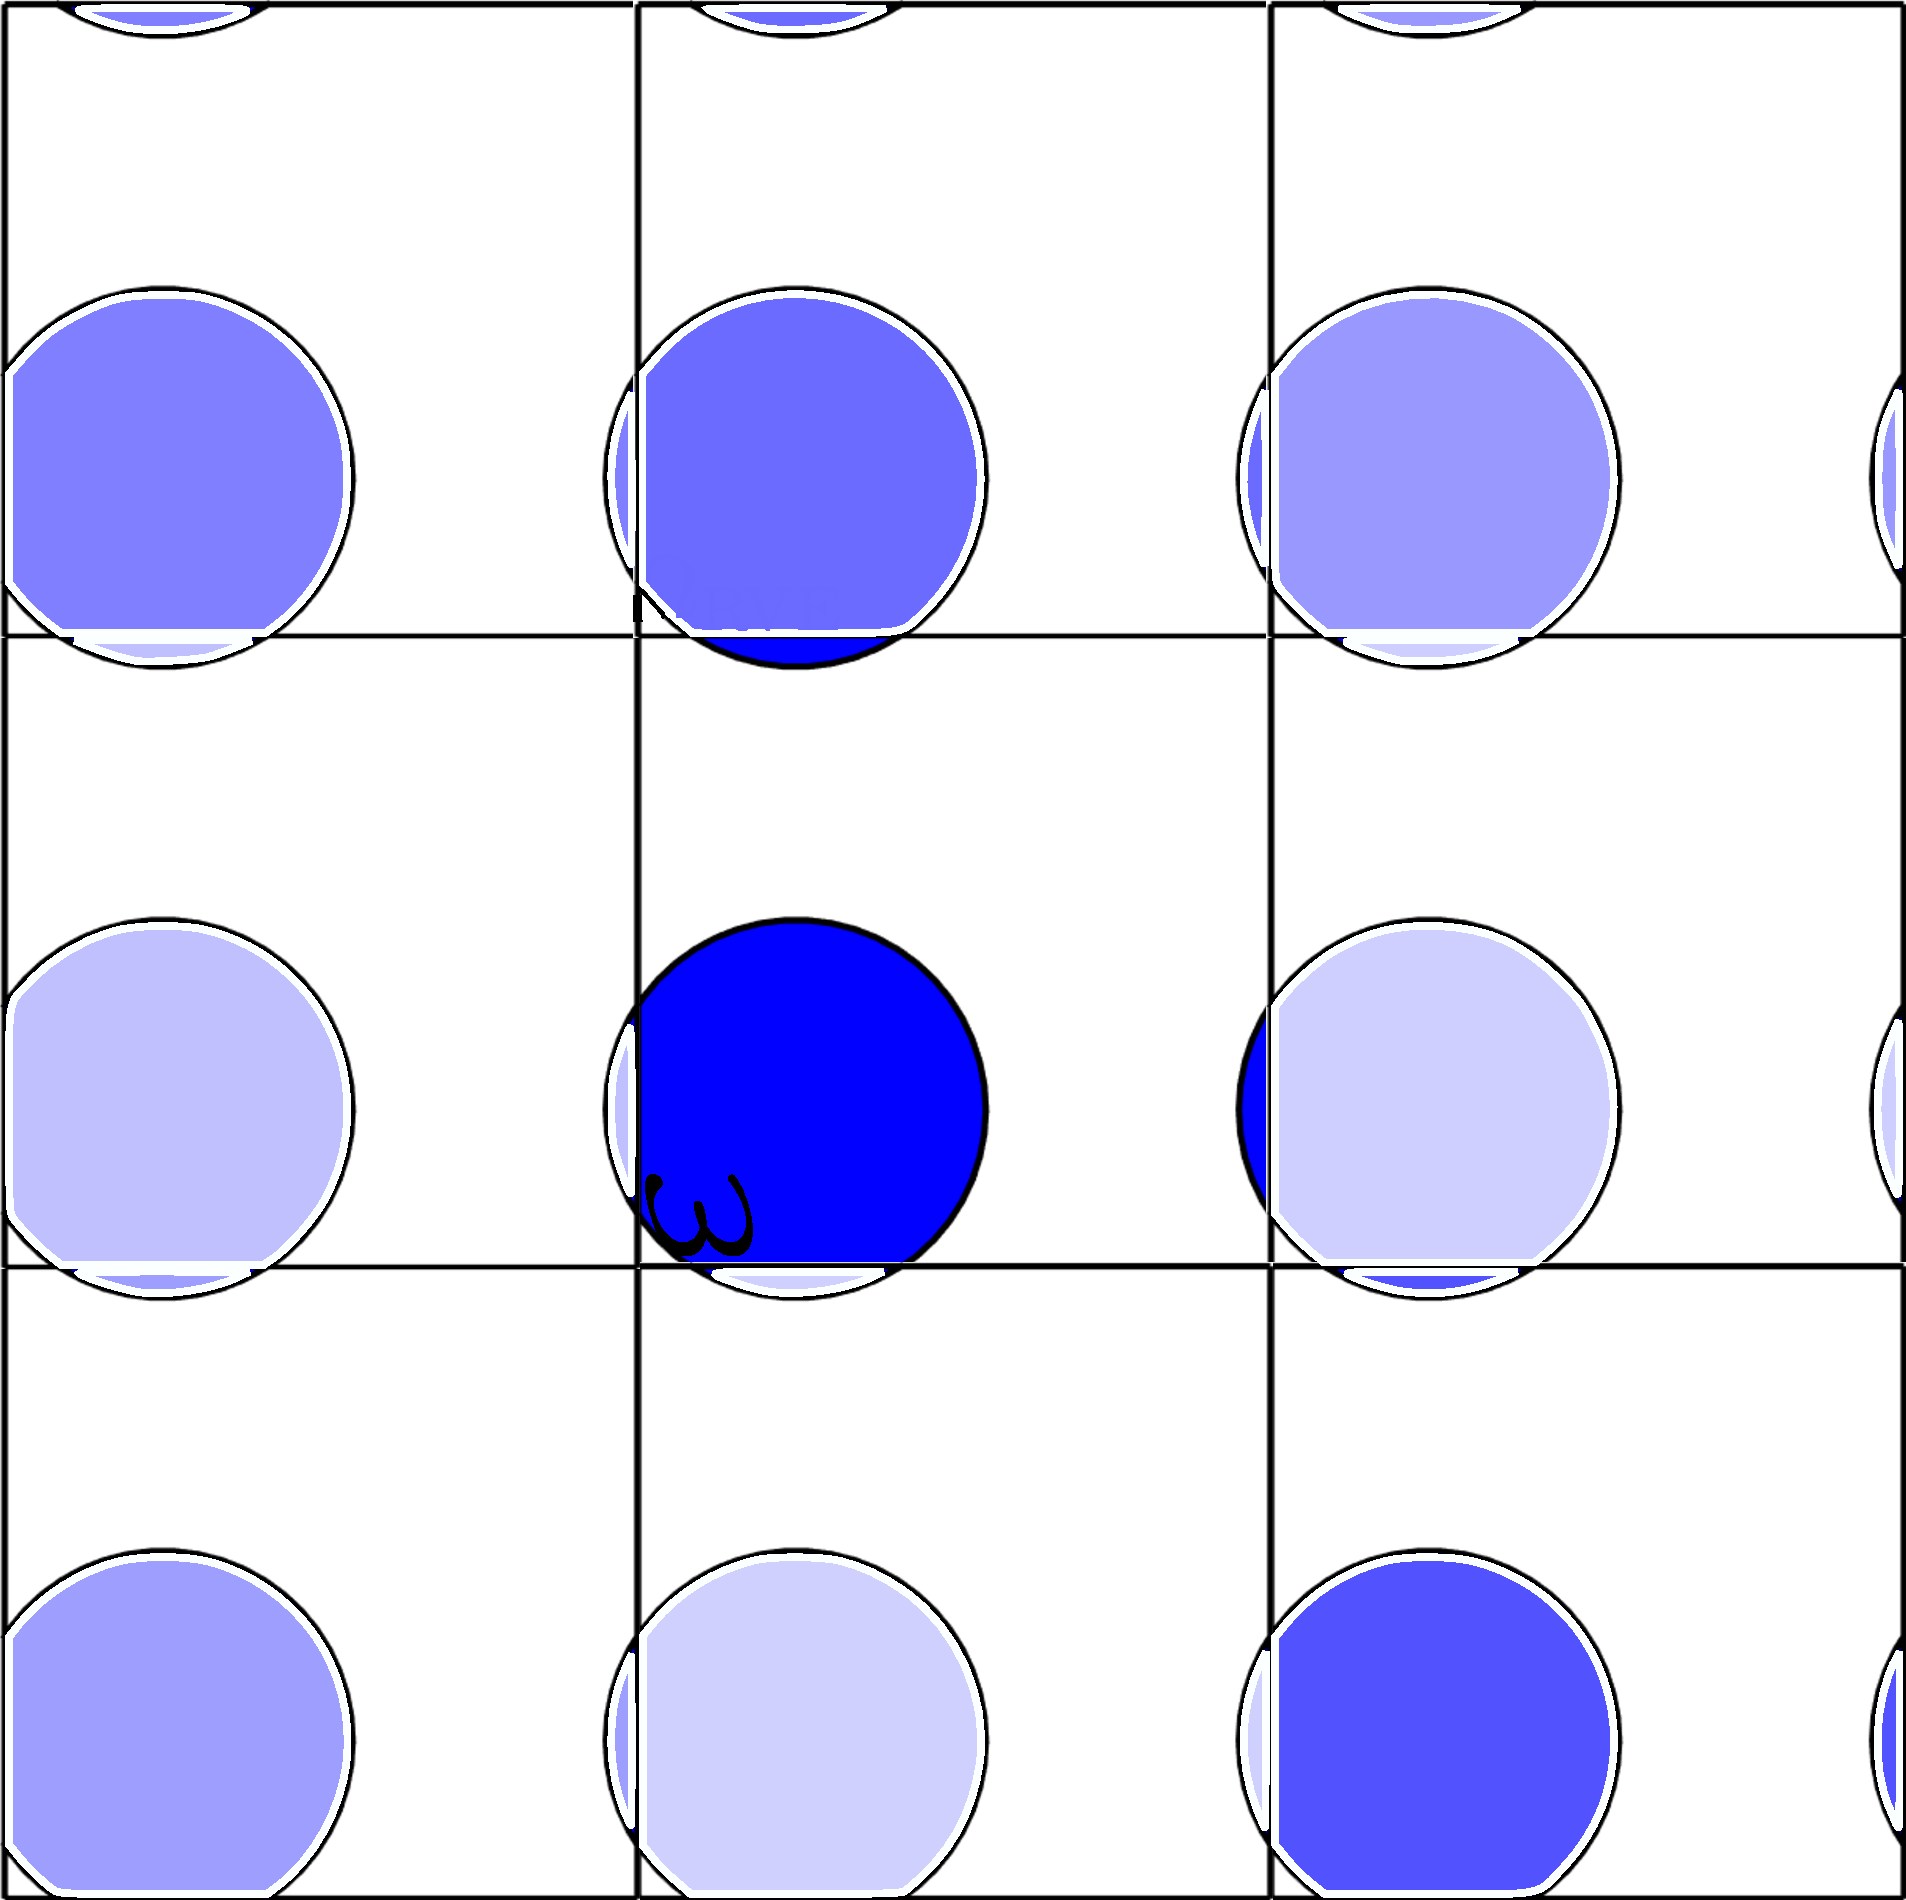
\includegraphics[width=\textwidth]{PER_2}
		\caption{}
	\end{subfigure}
	\begin{subfigure}[b]{0.32\textwidth}
		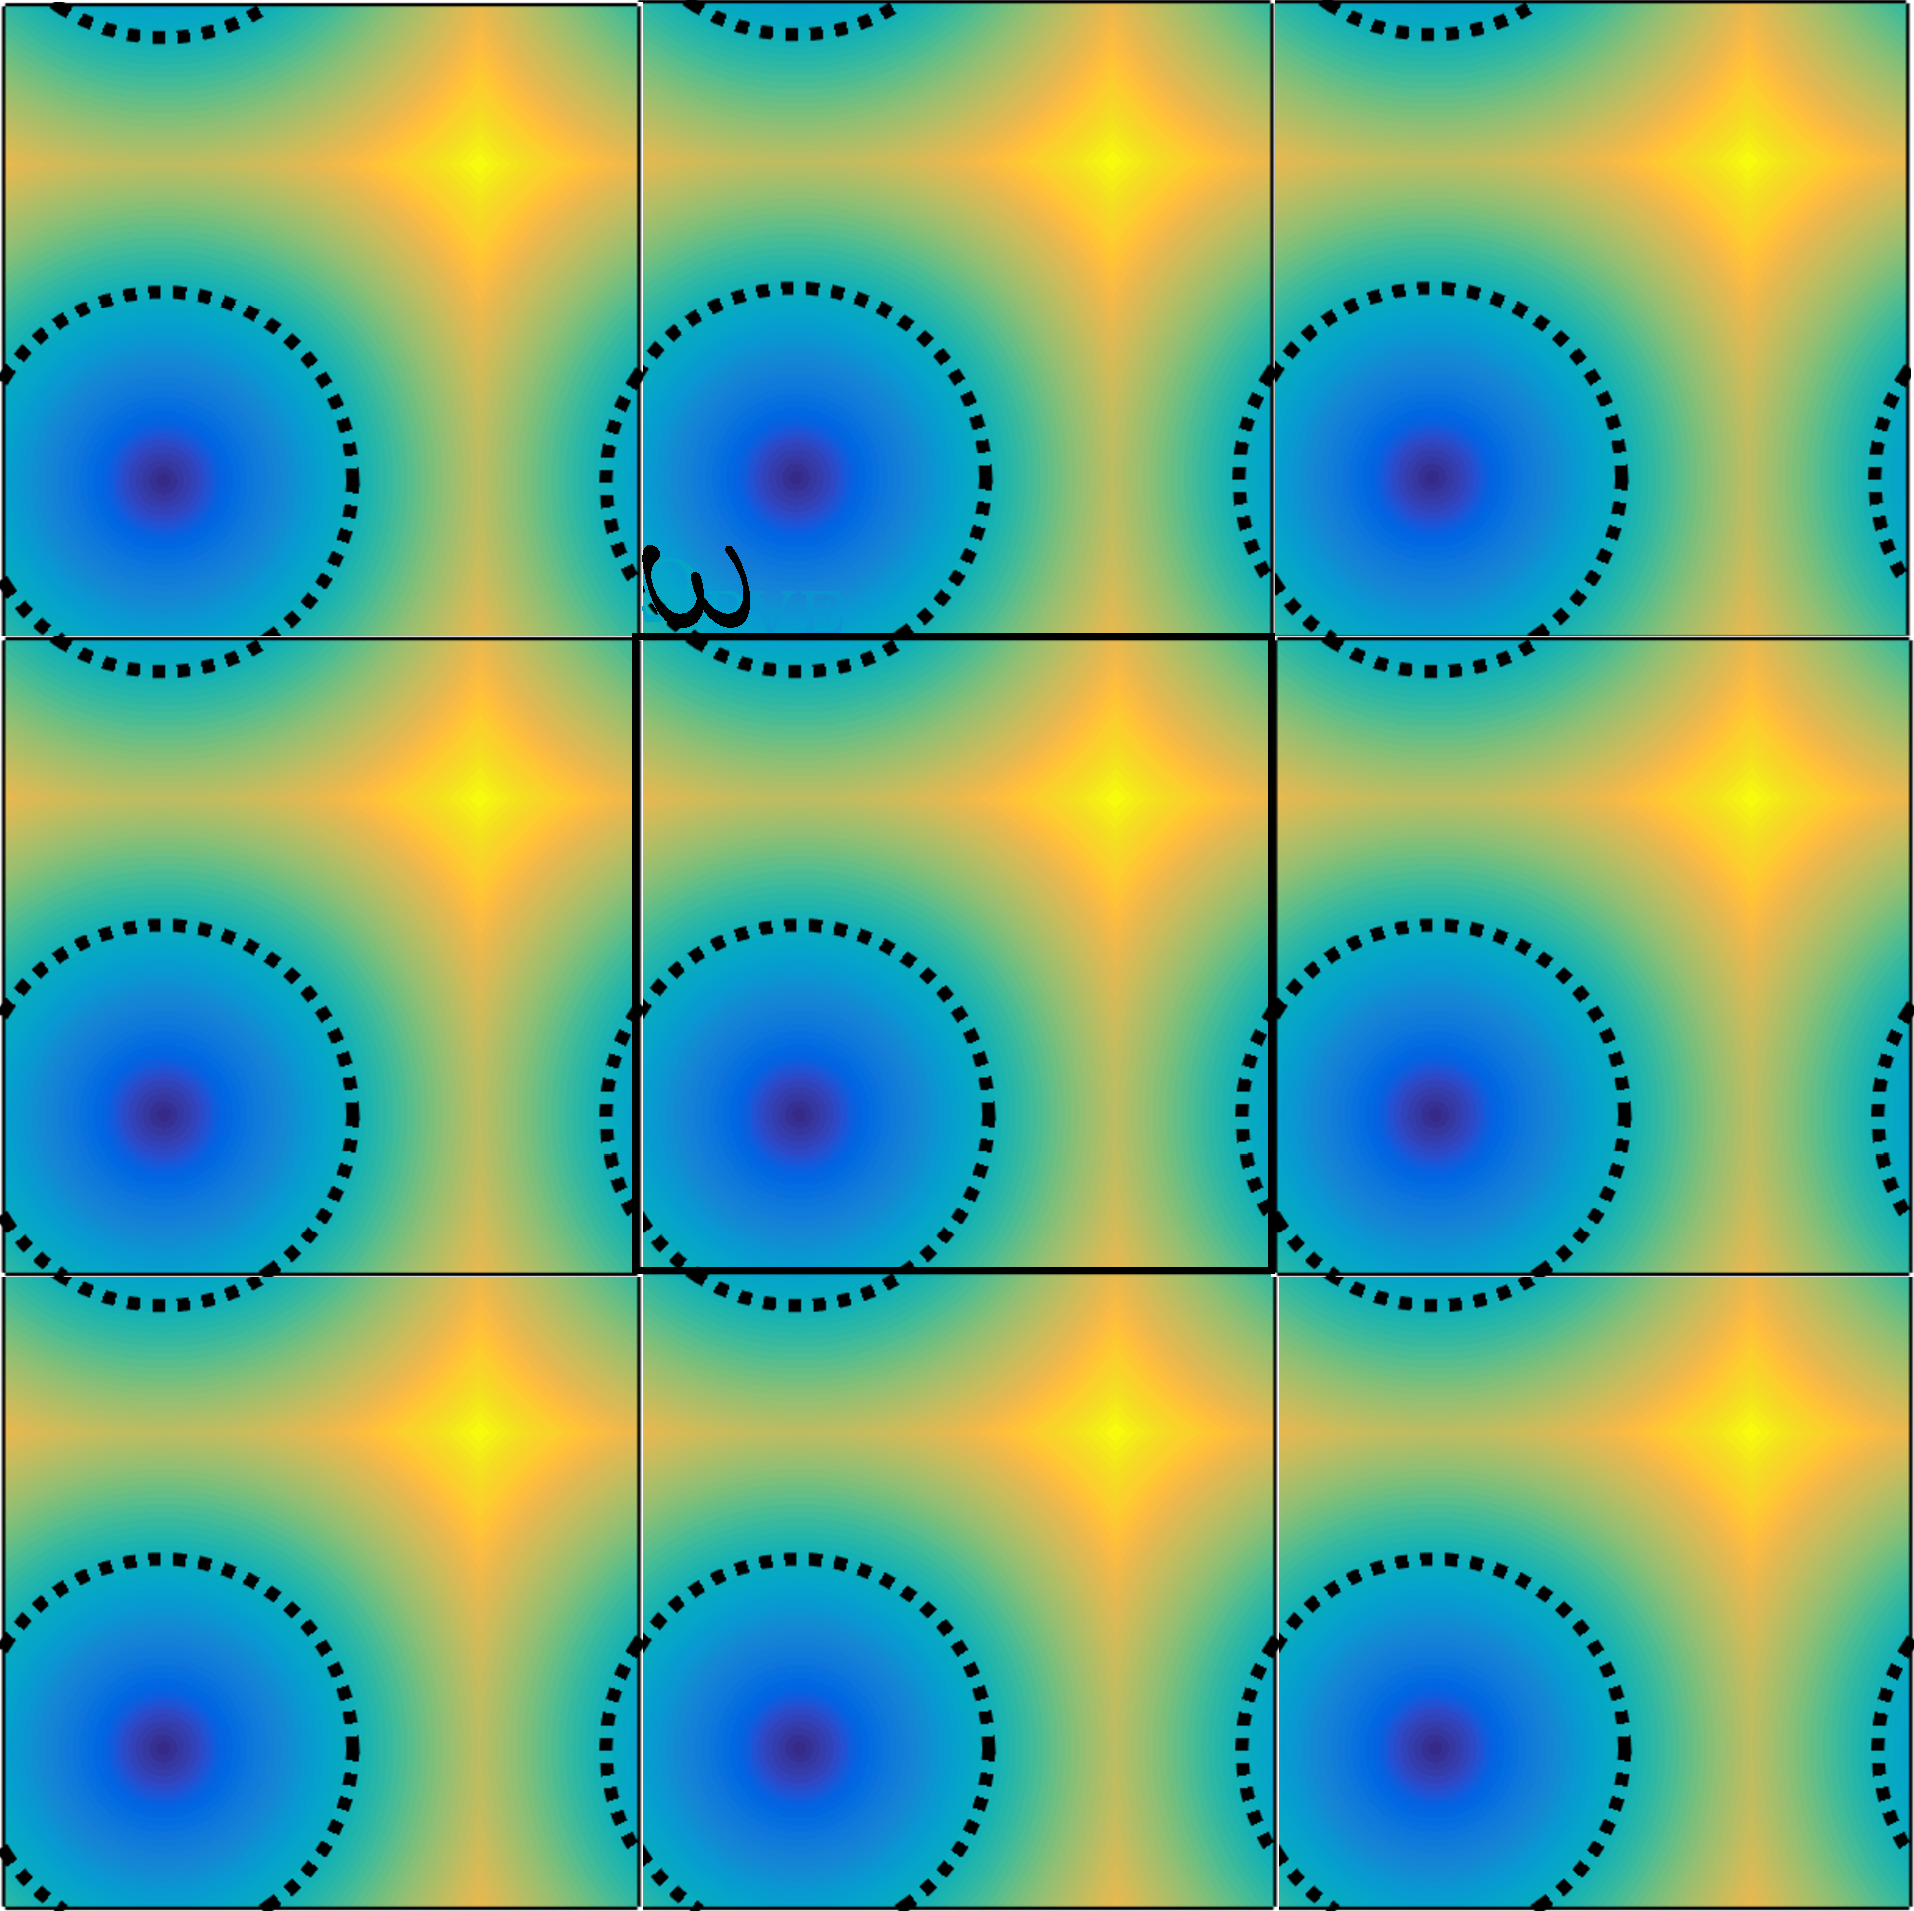
\includegraphics[width=\textwidth]{PER_1}
		\caption{}
	\end{subfigure}
	\caption{(a) Reproduction of an inclusion in its eight periodic neighbors; (b) $DN_1$ reproduction in the periodic setting. Periodicity is treated by extending the influence domain out of the RVE and by bringing them back in the RVE to its periodic location by translation.}\label{periodic}
\end{figure}

\begin{figure}
	\centering
	\begin{subfigure}[b]{0.32\textwidth}
		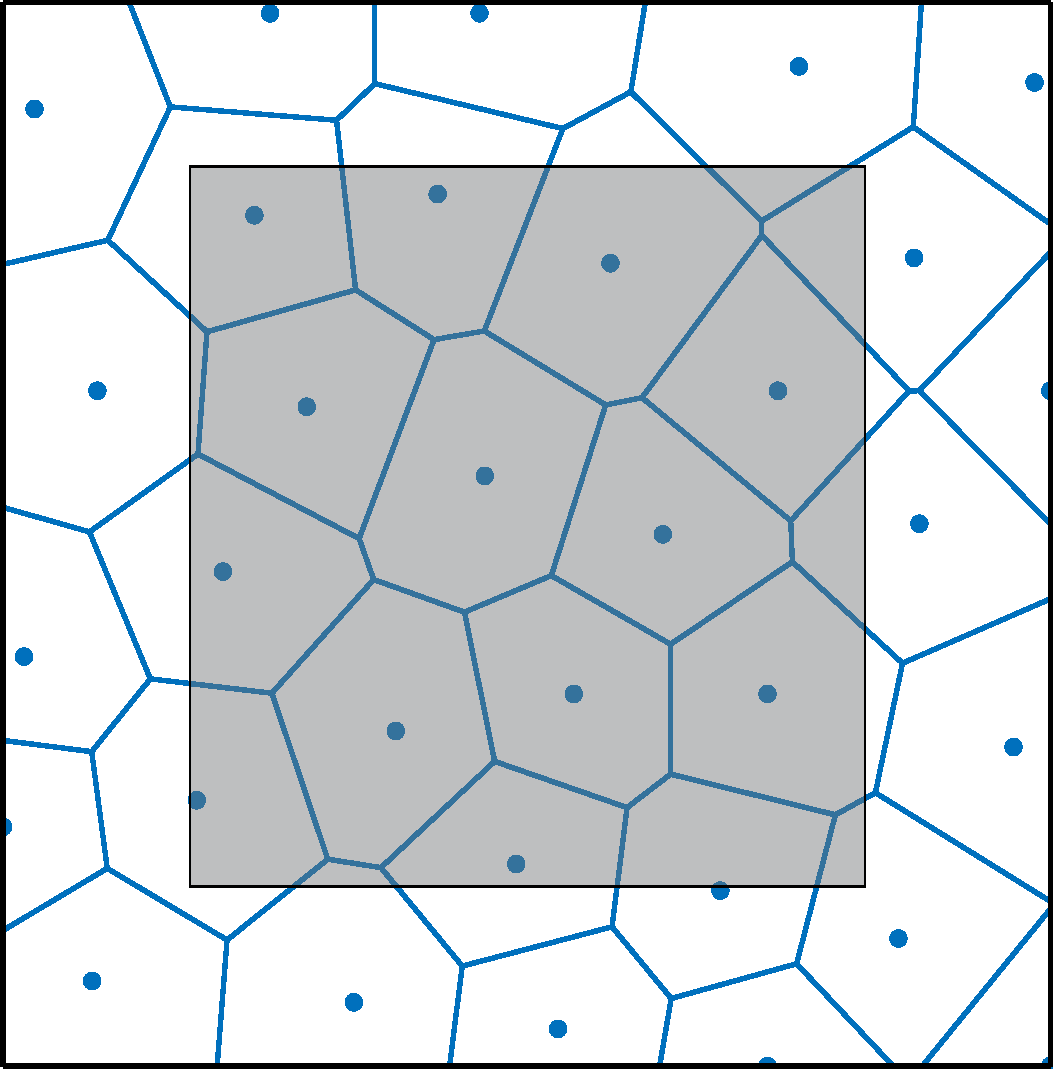
\includegraphics[width=\textwidth]{Minus_voronoi}
		\caption{}
	\end{subfigure}
	\begin{subfigure}[b]{0.327\textwidth}
		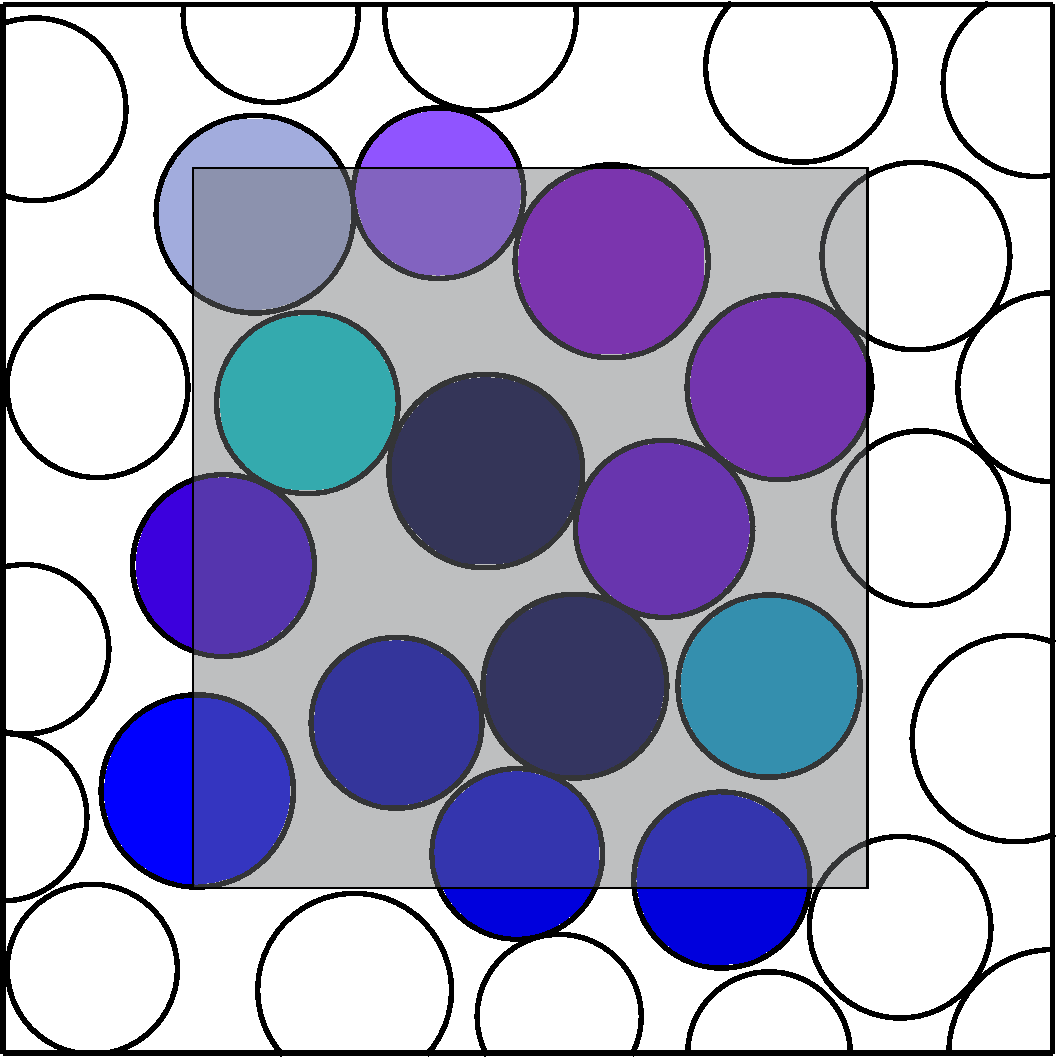
\includegraphics[width=\textwidth]{Minus_plt}
		\caption{}
	\end{subfigure}
	\caption{Minus sampling of free boundary RVE; (a) Only inclusions whose center lies within the domain definition are considered for treatment. (b) The new boundary of the domain and the objects that are taken into consideration.}\label{free}
\end{figure}

\subsection{``Vorono\"i'' and ``Plateau" level set functions}\label{of-gen-ov}
Classical tessellation patterns usually consist of tiling of a plane using multiple geometric shapes and the techniques used to generate these patterns gather cell points in each tessellation that are closer to a particular seed point. To this end, they require the use of distance measures. Every point in the domain will have one nearest seed, and consequently each seed has one sub-domain generated. This ensures that the sub-domains are exactly adjacent to each other. The Vorono\"i tessellation uses points as seeds and the Euclidean distance as distance measure with additively weighted Vorono\"i tessellation using circular/spherical seeds and Laguerre tessellation using circle/sphere power distance on a circular/spherical seeds\footnote{Concept of circle power based on the power of a point\cite{coxeterIntroductionGeometry1969}}. 
% Remark : Give explanation
The Laguerre tessellations are usually preferred as multi-sized cell tessellations (polydispersity) can be easily produced while keeping the cell faces plane and the edges of the cell faces straight (lack of edge curvature is an observed phenomenon in real foams \cite{andrewsCompressiveTensileBehaviour1999}).

With the help of notations in Figure \ref{omega}, from a given inclusion packing generated by DN-RSA, it is possible to define a tessellation made of the assembly of all $ ^I\Theta_i $ domains which degenerates in a Laguerre tessellation for multi-sized sphere packings. This tessellation can be constructed implicitly with the first and the second neighbor distance fields of the initial inclusion packing by a ``Vorono\"i'' level set function defined as:
\begin{equation}
O_V(\textbf{x})=DN_2(\textbf{x})-DN_1(\textbf{x})\label{voronoi-1}.
\end{equation}
The value of this function is exactly zero at loci equidistant from two nearest inclusions, i.e. on the faces of the tessellations, and is positive everywhere else, as it can be seen in Figure \ref{voronoi1}a for a 2D example. A quasi constant thickness, $ t $, can be used in combination with $ O_V $ to extract a closed cell geometry through level sets:
\begin{equation}
O_V(\textbf{x})-t=0\label{voronoi}.
\end{equation}
Figure \ref{voronoi1}b also illustrates this relation in 2D. Figure \ref{voronoi2}a illustrates a packing generated in 3D, with the corresponding RVE generated by the use of Eq. (\ref{voronoi}) in Figure \ref{voronoi2}b.

\begin{figure}
	\centering
	\begin{subfigure}[b]{0.32\textwidth}
		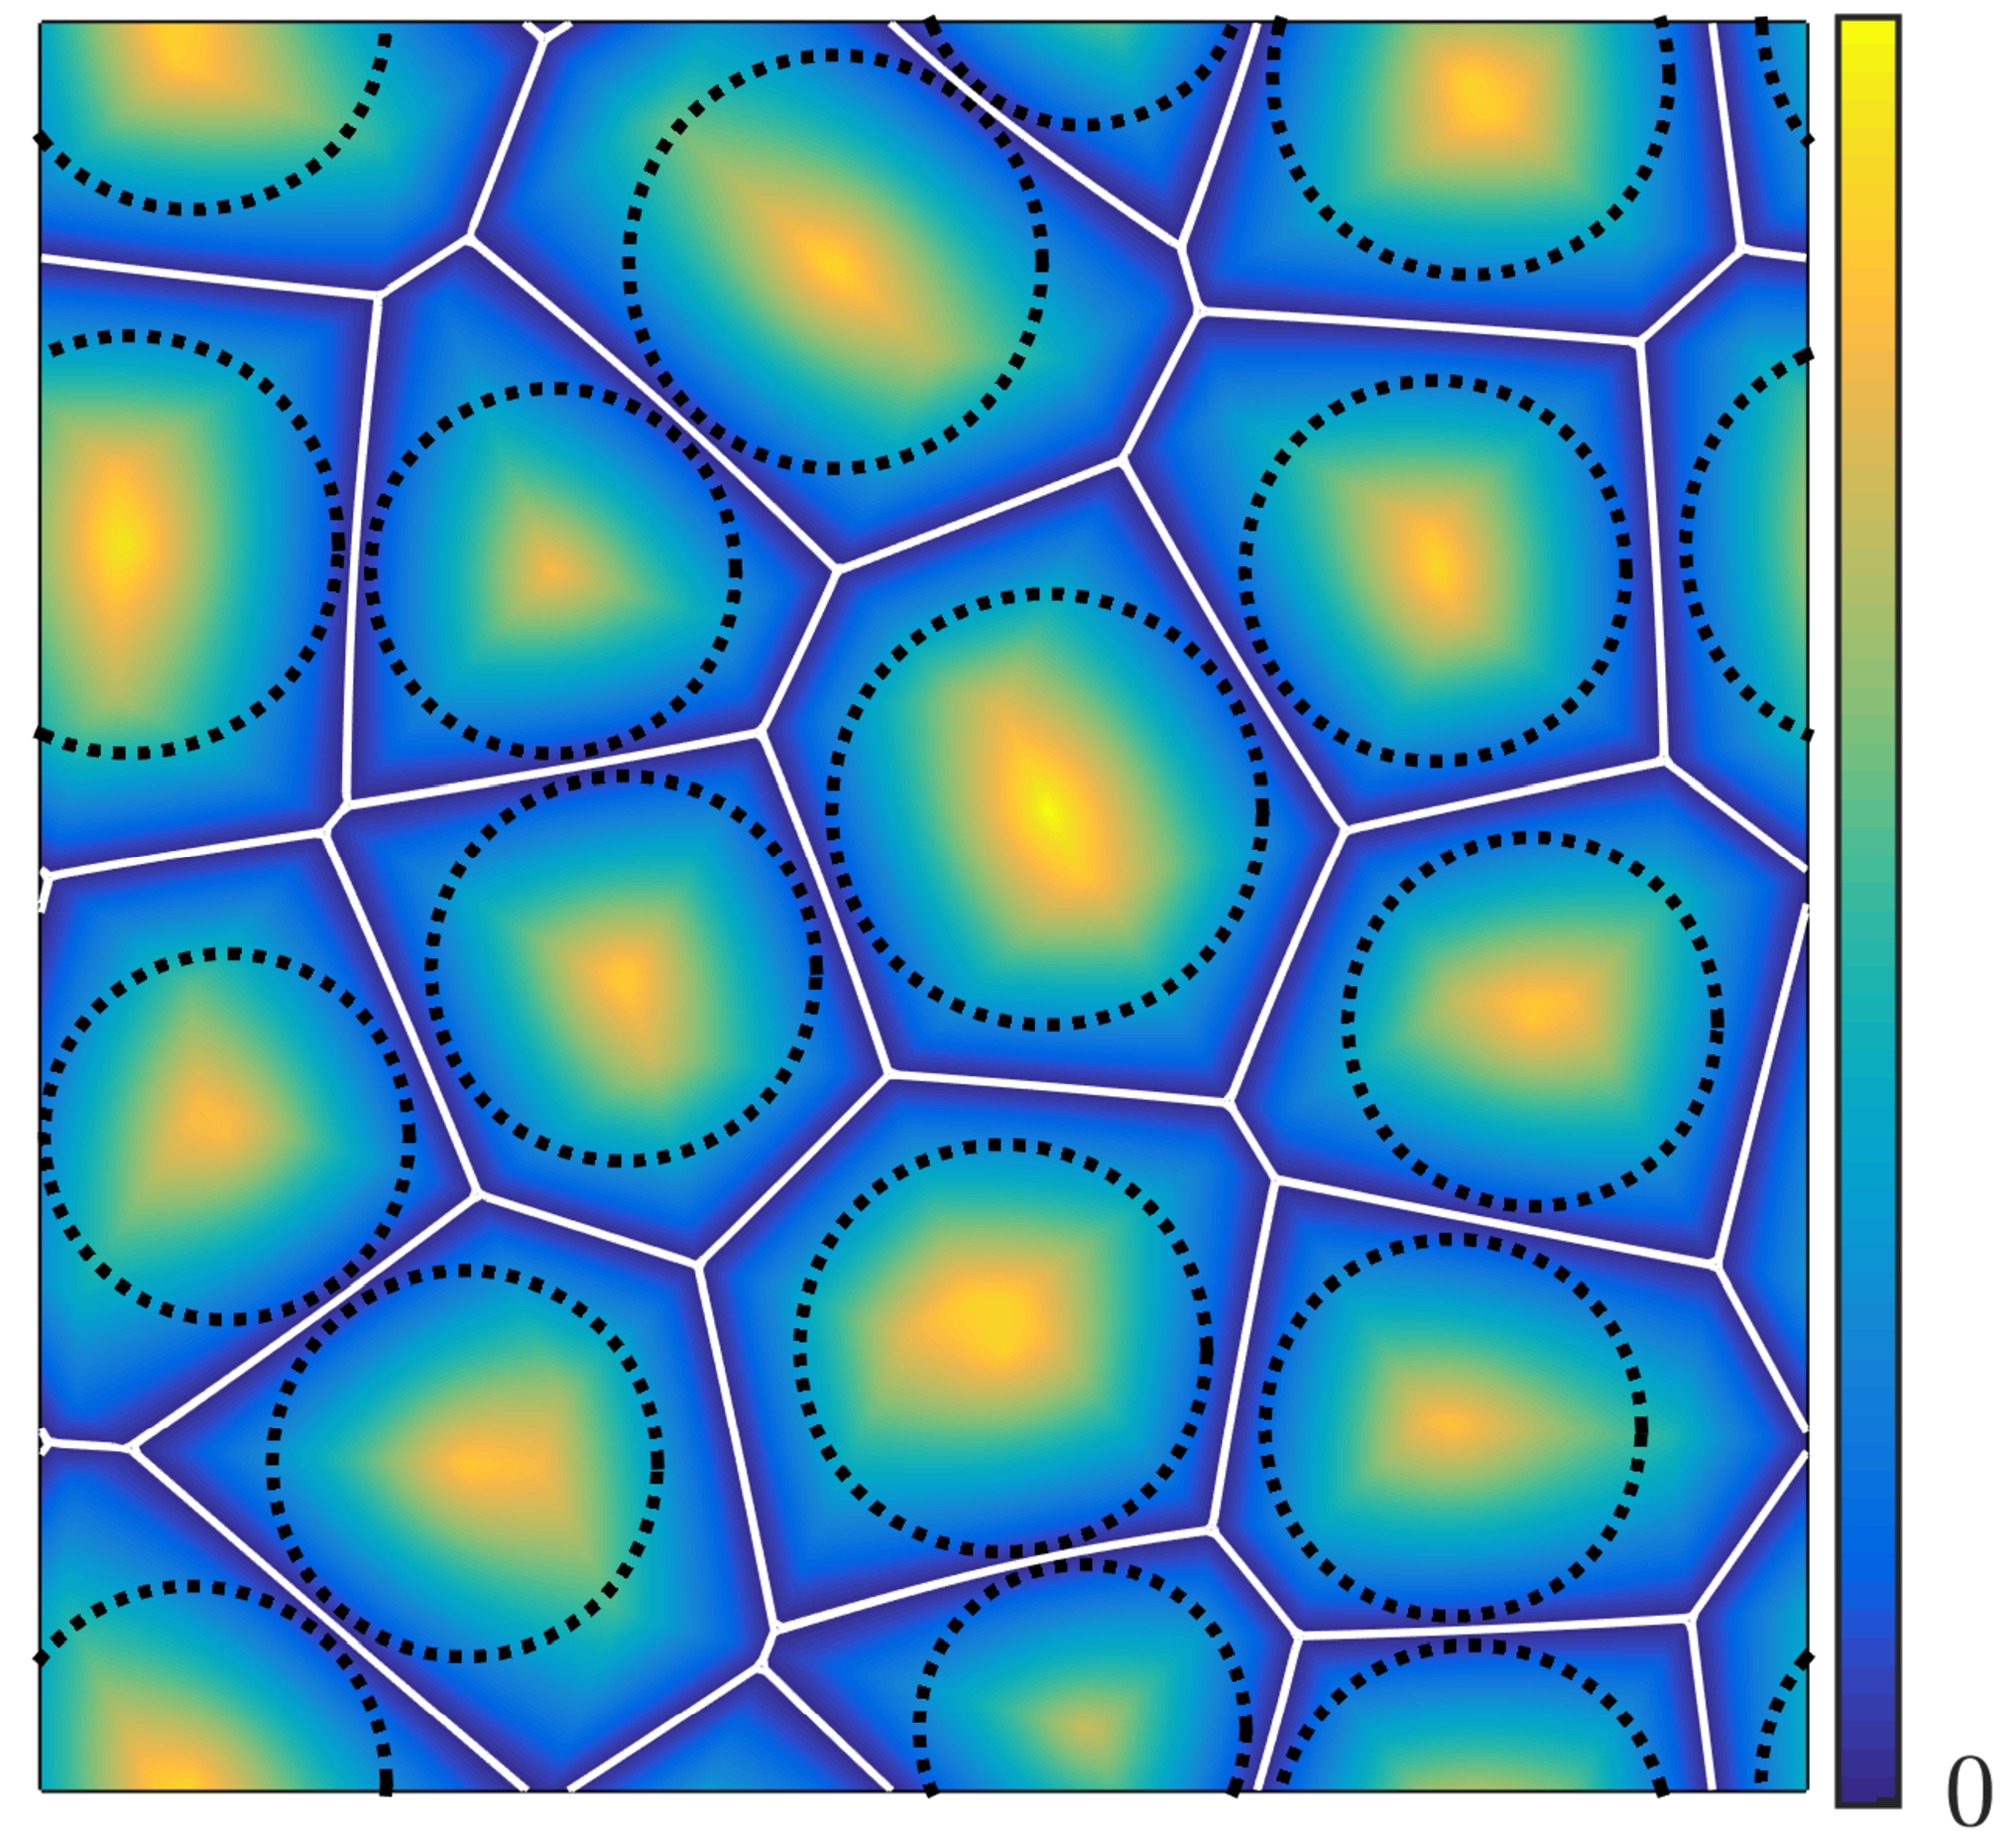
\includegraphics[width=\textwidth]{OV}
		\caption{}
	\end{subfigure}
	\begin{subfigure}[b]{0.32\textwidth}
		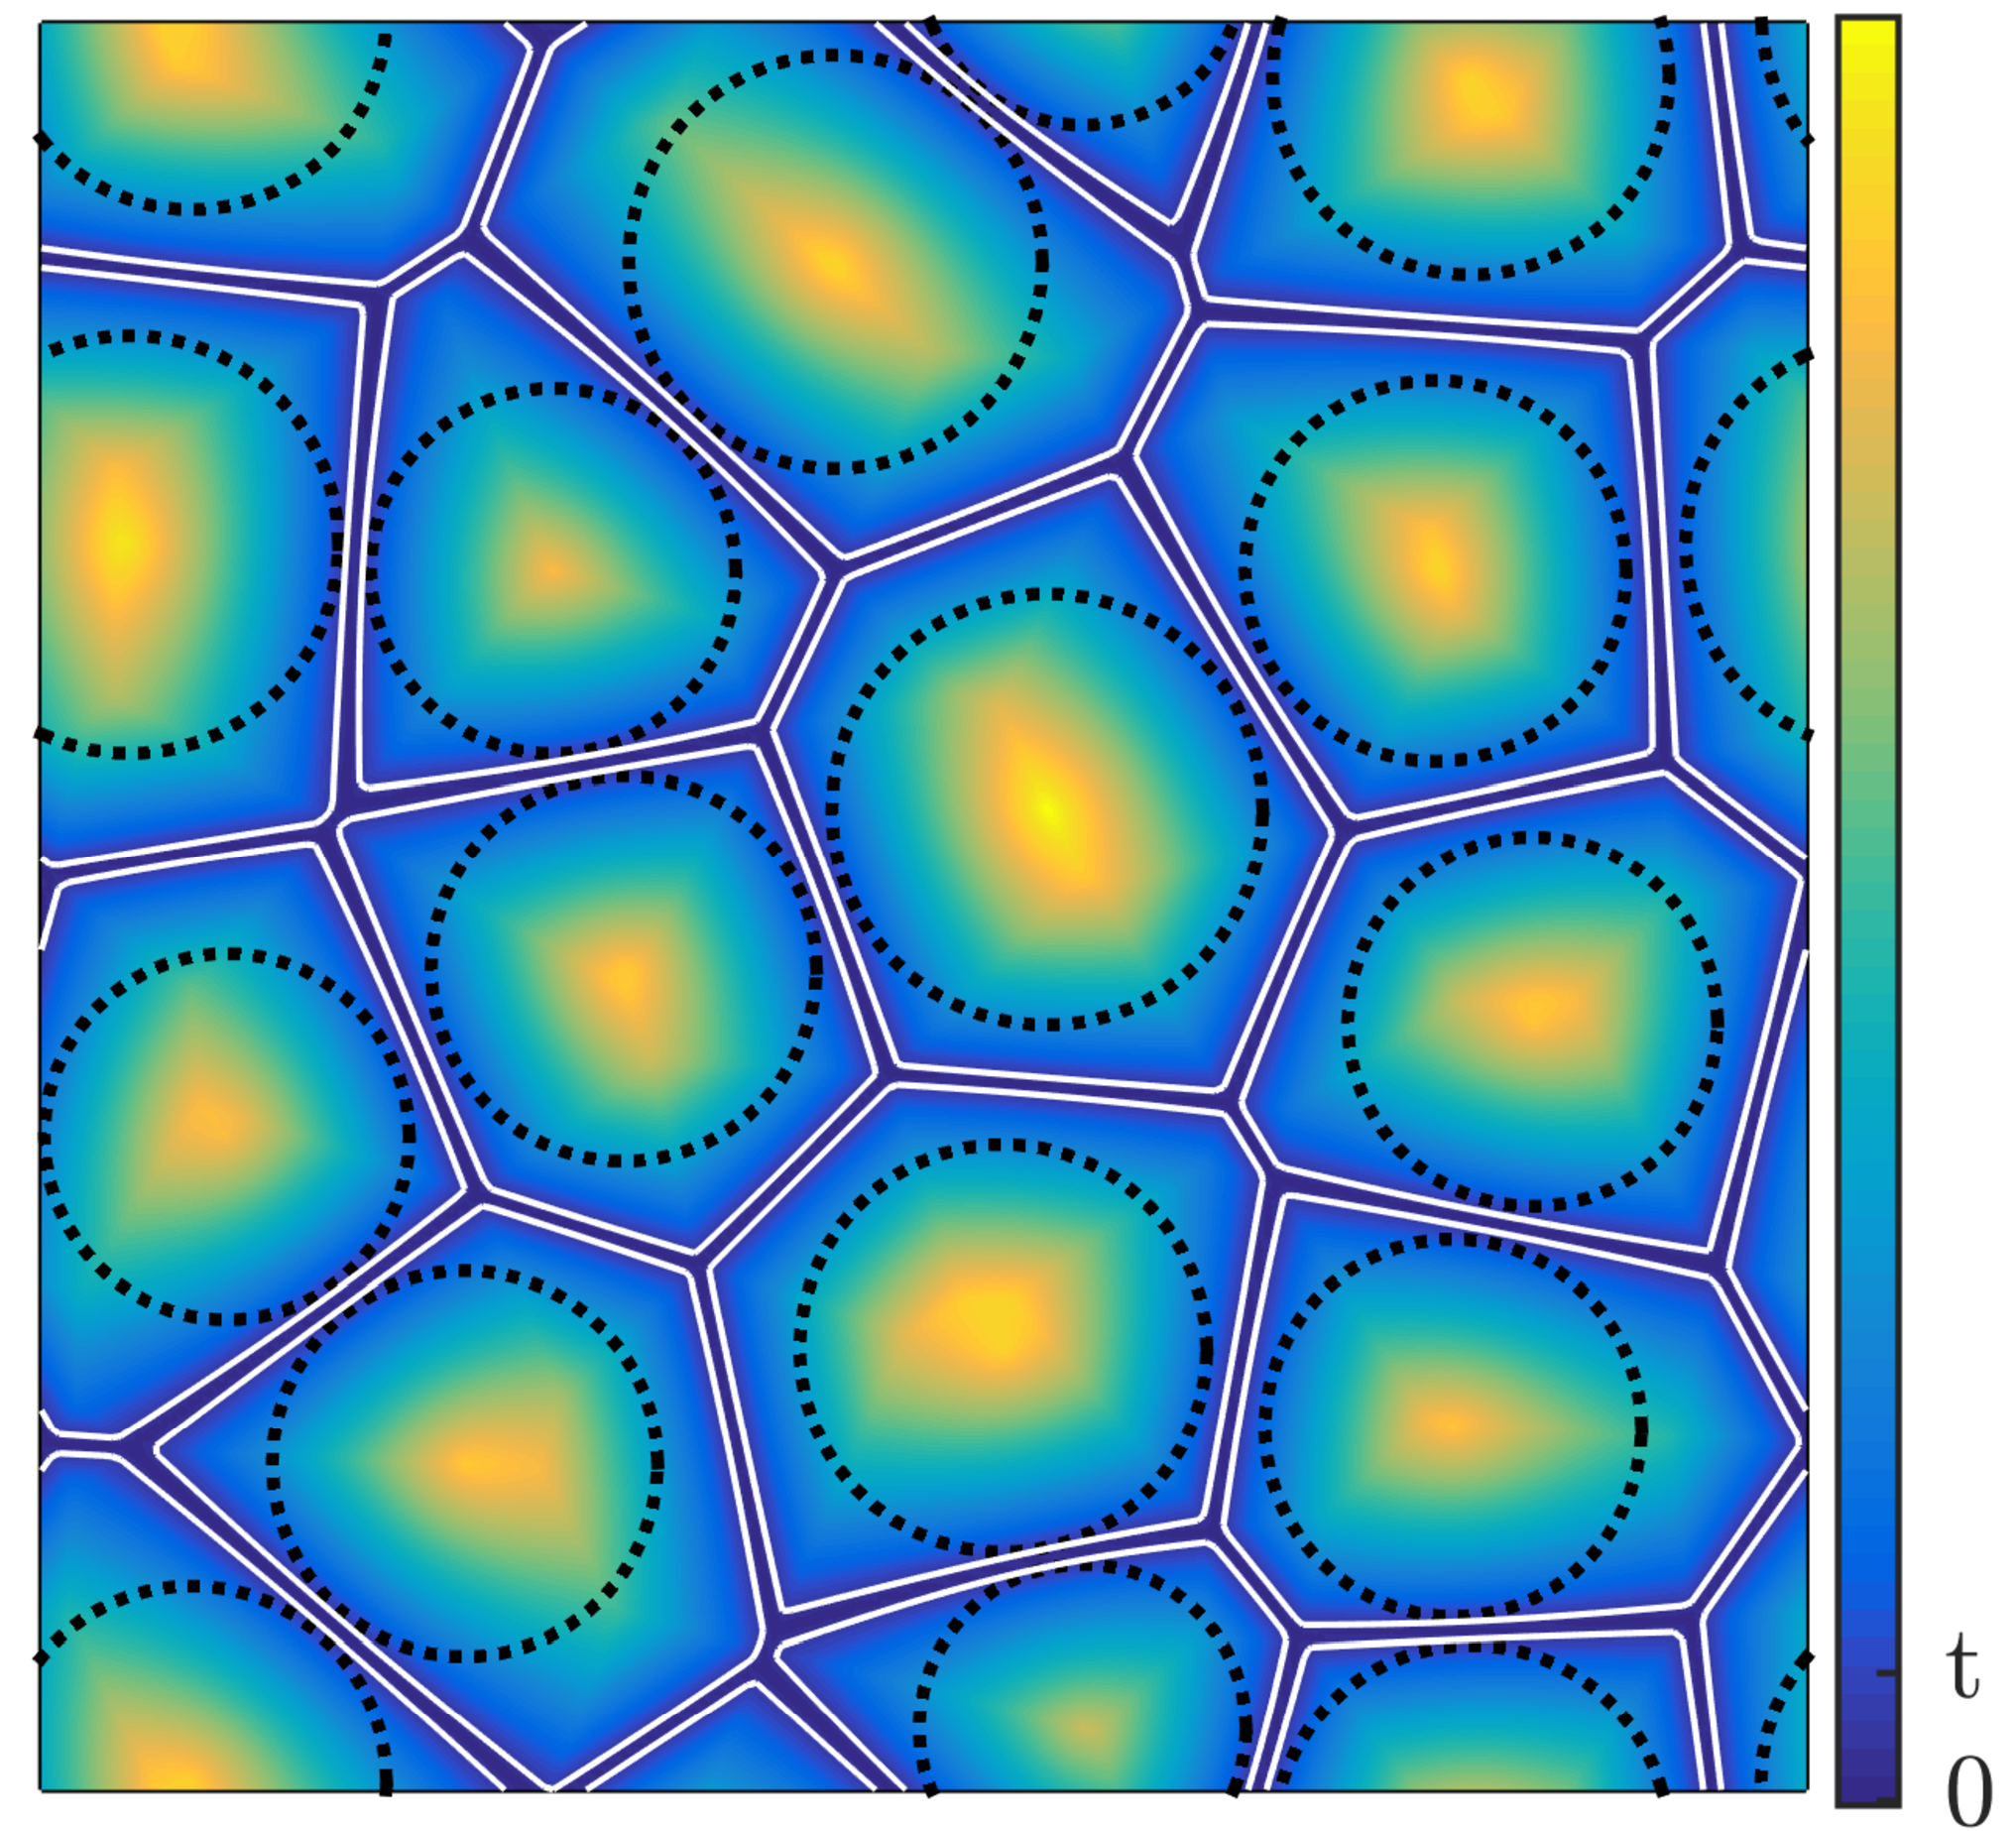
\includegraphics[width=\textwidth]{OV_t}
		\caption{}
	\end{subfigure}
	\caption{Vorono\"i level set functions for disk packings; (a) From Eq. (\ref{voronoi-1}), and (b) following Eq. (\ref{voronoi}) with $ t=0.01 $.}\label{voronoi1}
\end{figure}

\begin{figure}
	\centering
	\begin{subfigure}[b]{0.32\textwidth}
		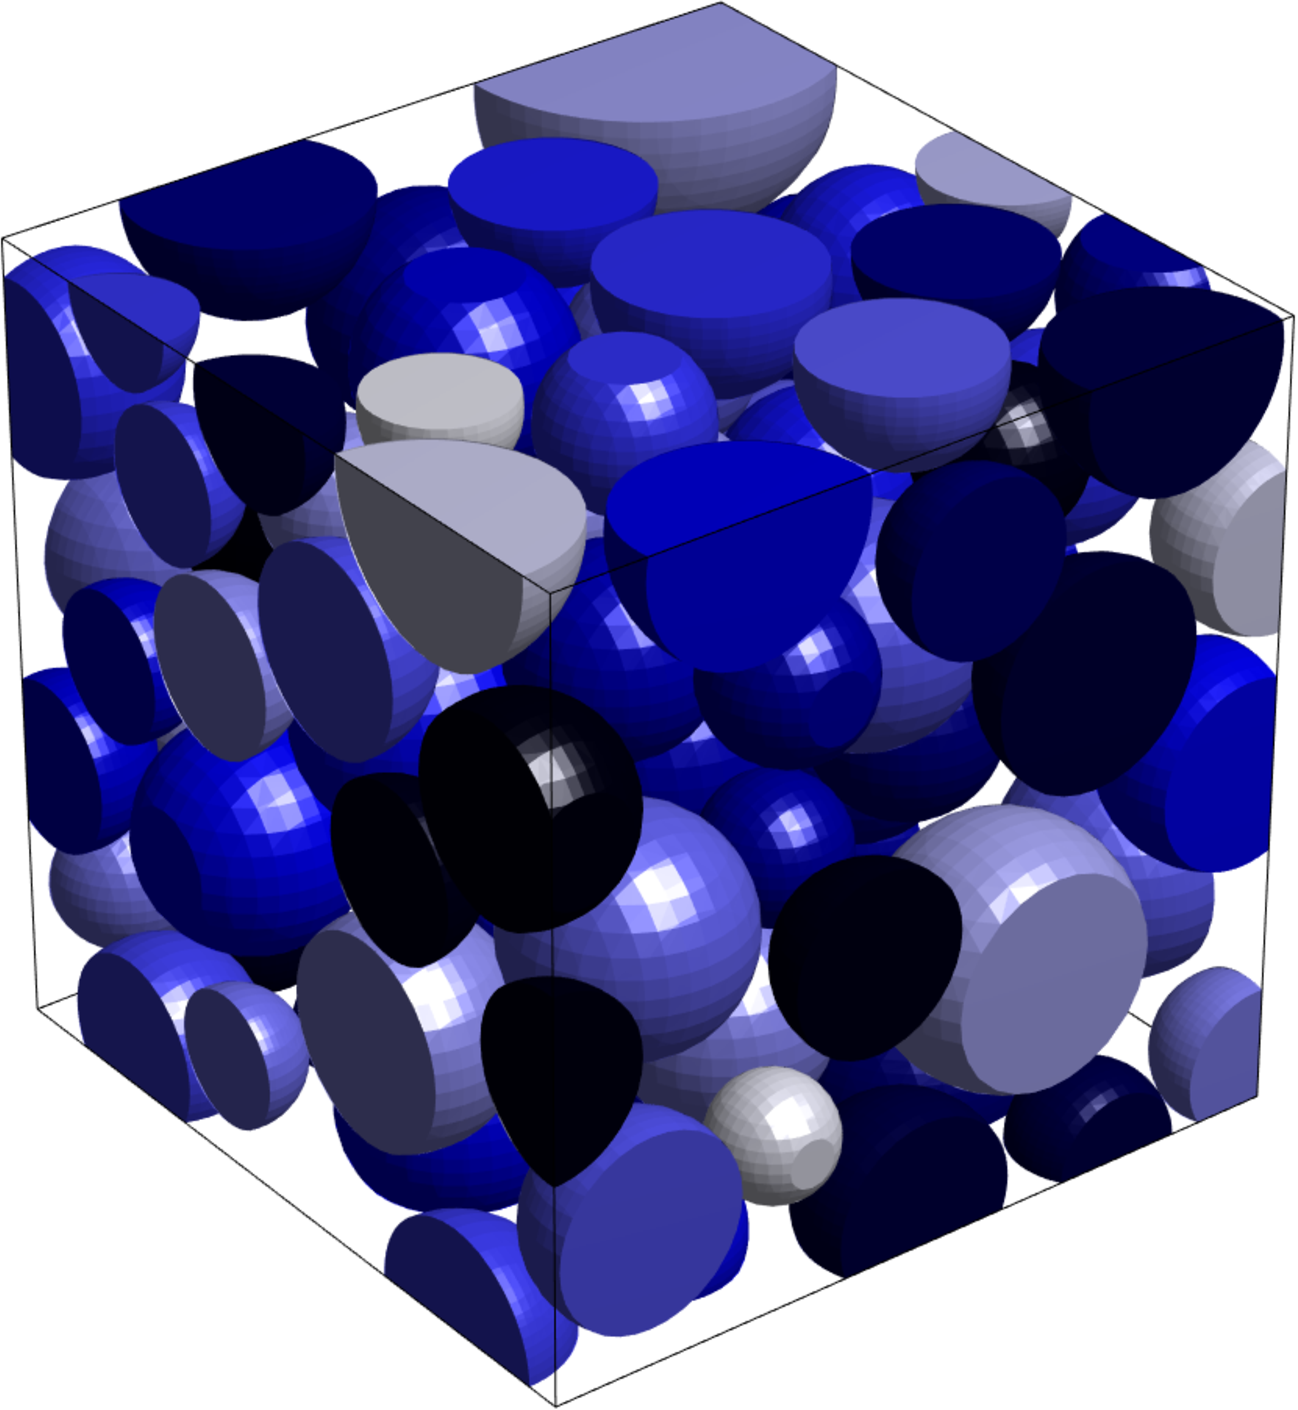
\includegraphics[width=\textwidth]{OV_pack}
		\caption{}
	\end{subfigure}
	\begin{subfigure}[b]{0.32\textwidth}
		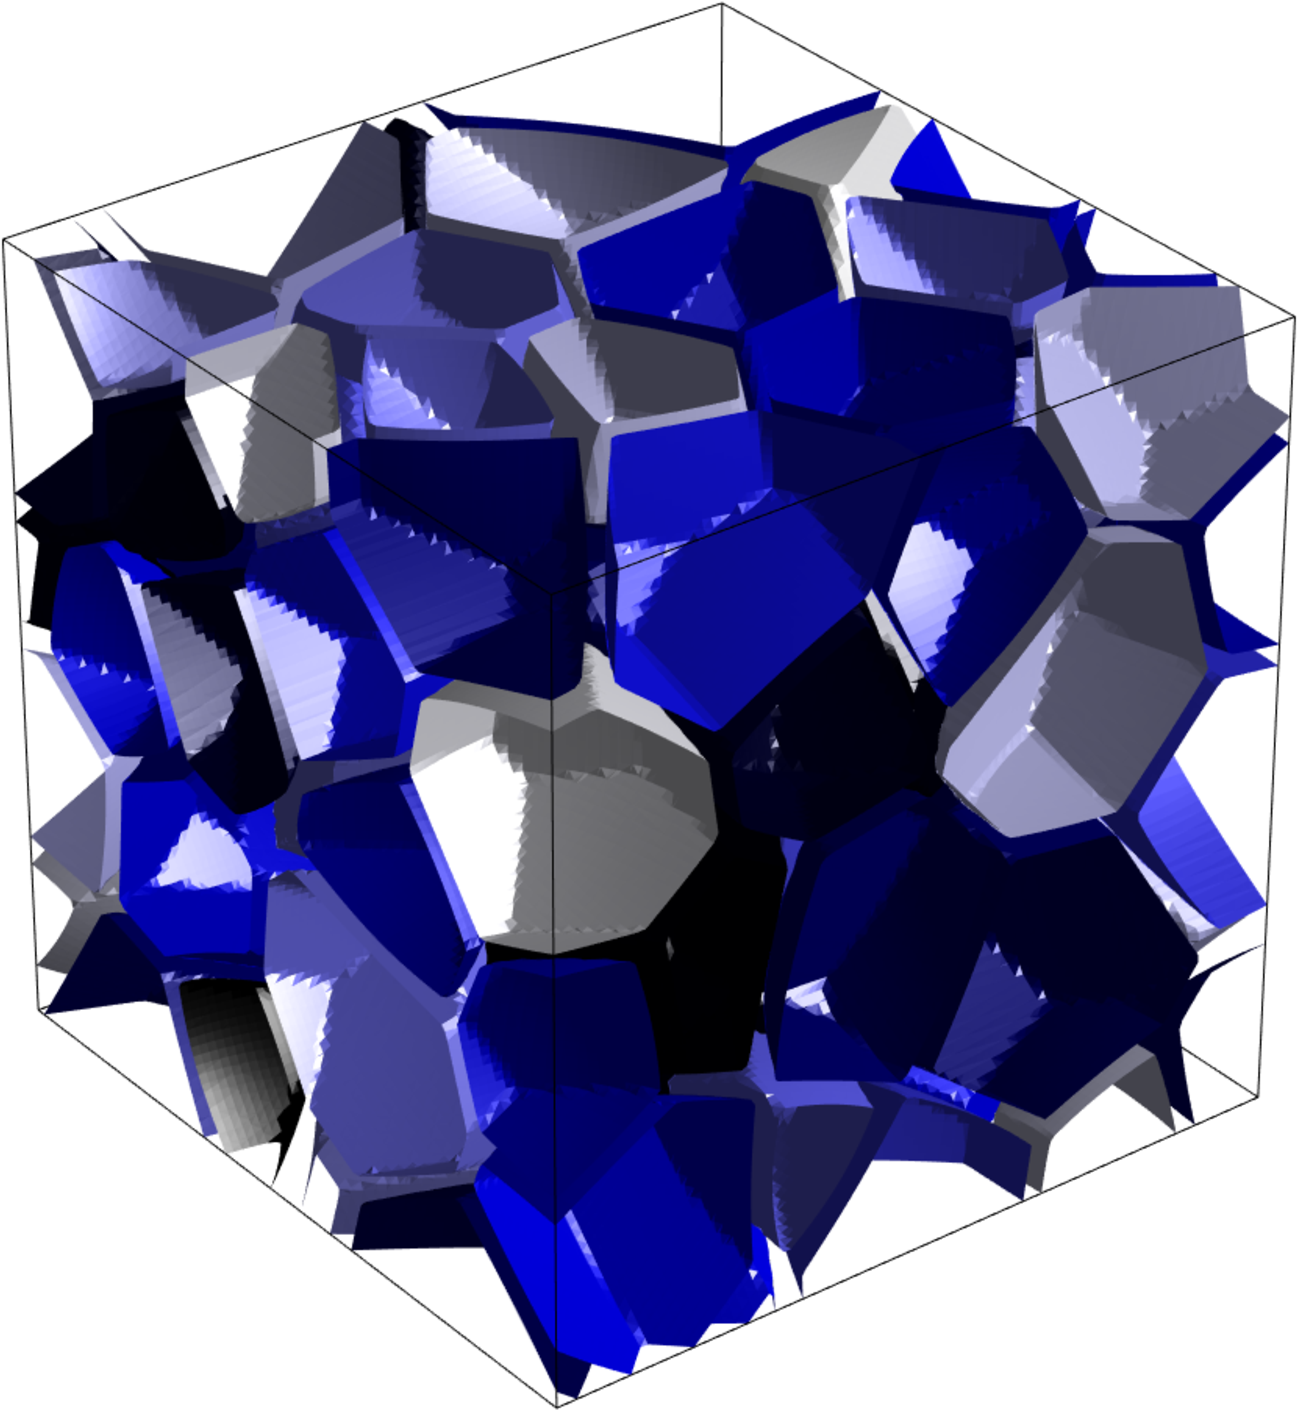
\includegraphics[width=\textwidth]{OV_tess}
		\caption{}
	\end{subfigure}
	\caption{(a) A multi-sized sphere packing, and (b) a closed cell RVE generated from the packing with $ t=0.025 $.}\label{voronoi2}
\end{figure}

Open foam micro-structures can be defined by the interlinking of 3D struts, usually with a triangular cross-section. An ad-hoc level set function can be defined in order to extract such struts from the edges of the tessellation. Using the first three neighbor distance functions, and taking inspiration from the knowledge that Plateau borders in liquid foams form at the intersection of three films, a relevant function denoted as the ``Plateau" level set function can be defined as\cite{sononAdvancedApproachGeneration2015}:
\begin{equation}
O_P(\textbf{x})=\frac{(DN_3(\textbf{x})+DN_2(\textbf{x}))}{2}-DN_1(\textbf{x})\,.\label{OP}
\end{equation}
This function vanishes at the locus where the distance from the three nearest inclusions is the same, and is positive everywhere else.

The level set of this function consists of triangles with vertex lying on the tessellation cell boundaries. A natural way of extracting a Plateau border like geometry is therefore given by
\begin{equation}
O_P(\textbf{x})-t=0\,,\label{OP-2}
\end{equation}
where the parameter $ t $ controls the thickness of the extracted boundary (Figure \ref{plateau11}). This thickness is related to the parameter in Eq. (\ref{voronoi}) such that the plateau borders produced can be completely contained in the corresponding closed cell walls (Figure \ref{plateau1}). 

\begin{figure}
	\centering
	\begin{subfigure}[b]{0.33\textwidth}
		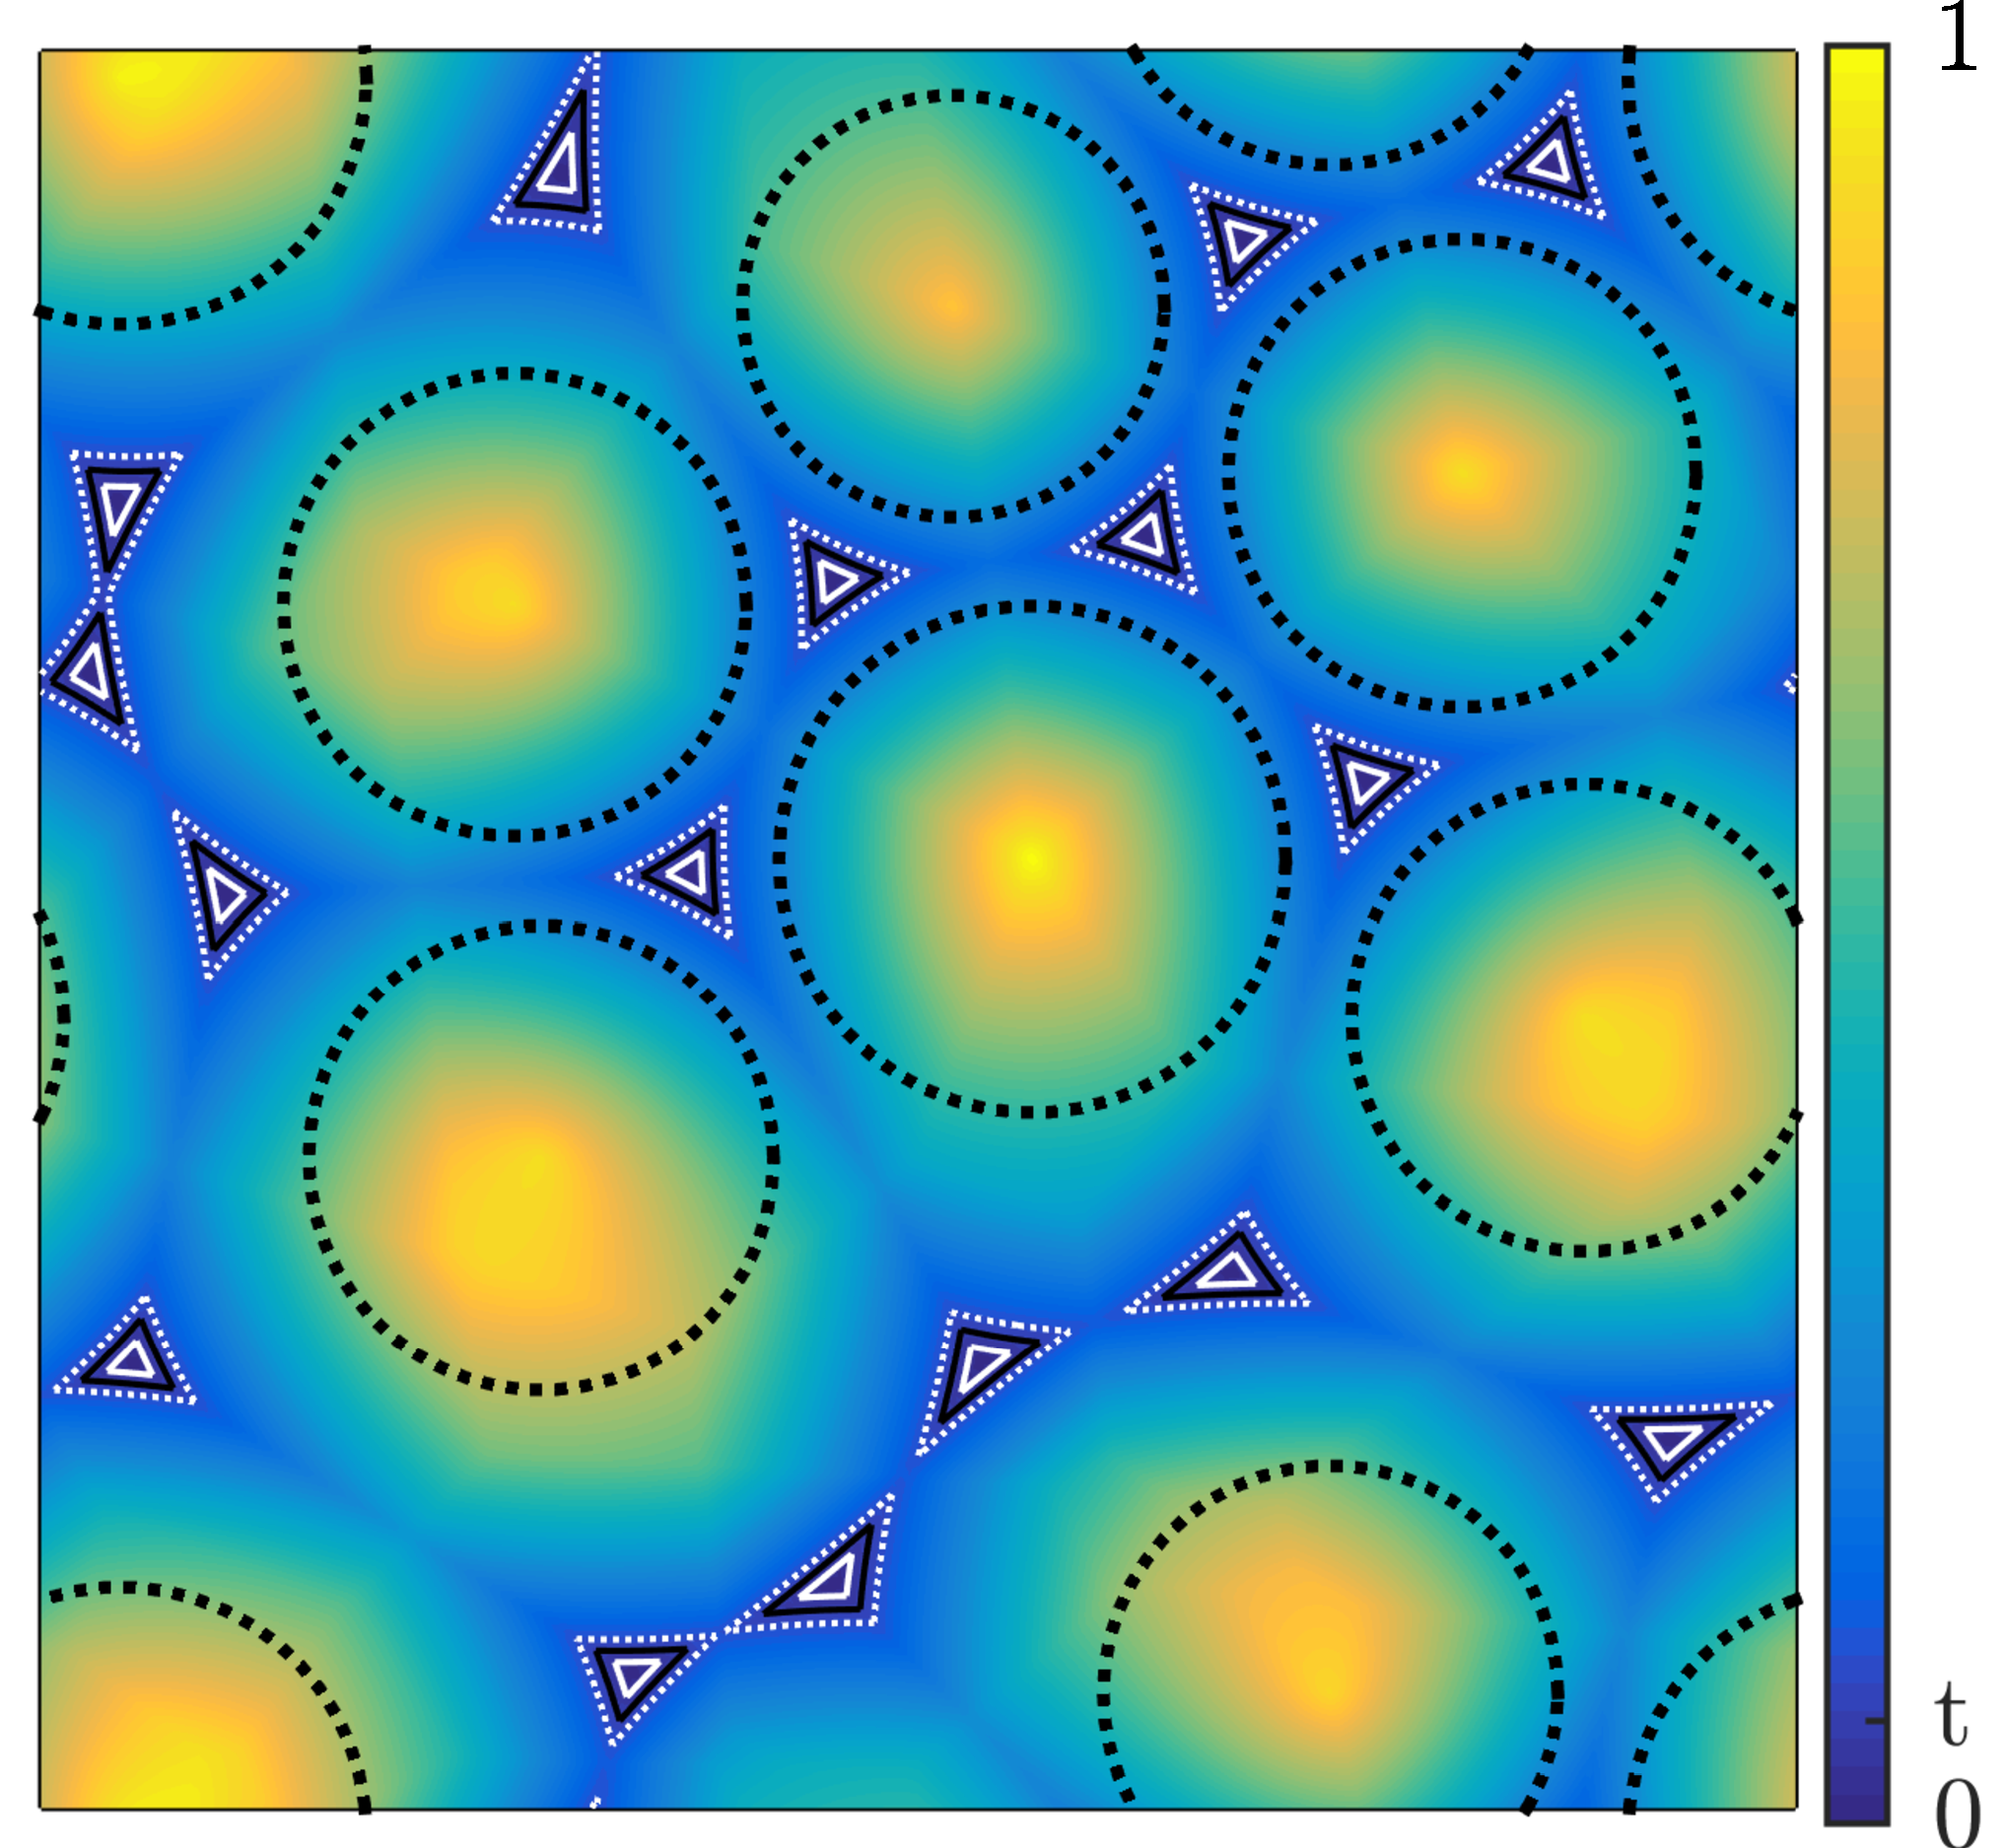
\includegraphics[width=\textwidth]{OP_MULTIPLE}
		\caption{}\label{plateau11}
	\end{subfigure}
	\begin{subfigure}[b]{0.3\textwidth}
		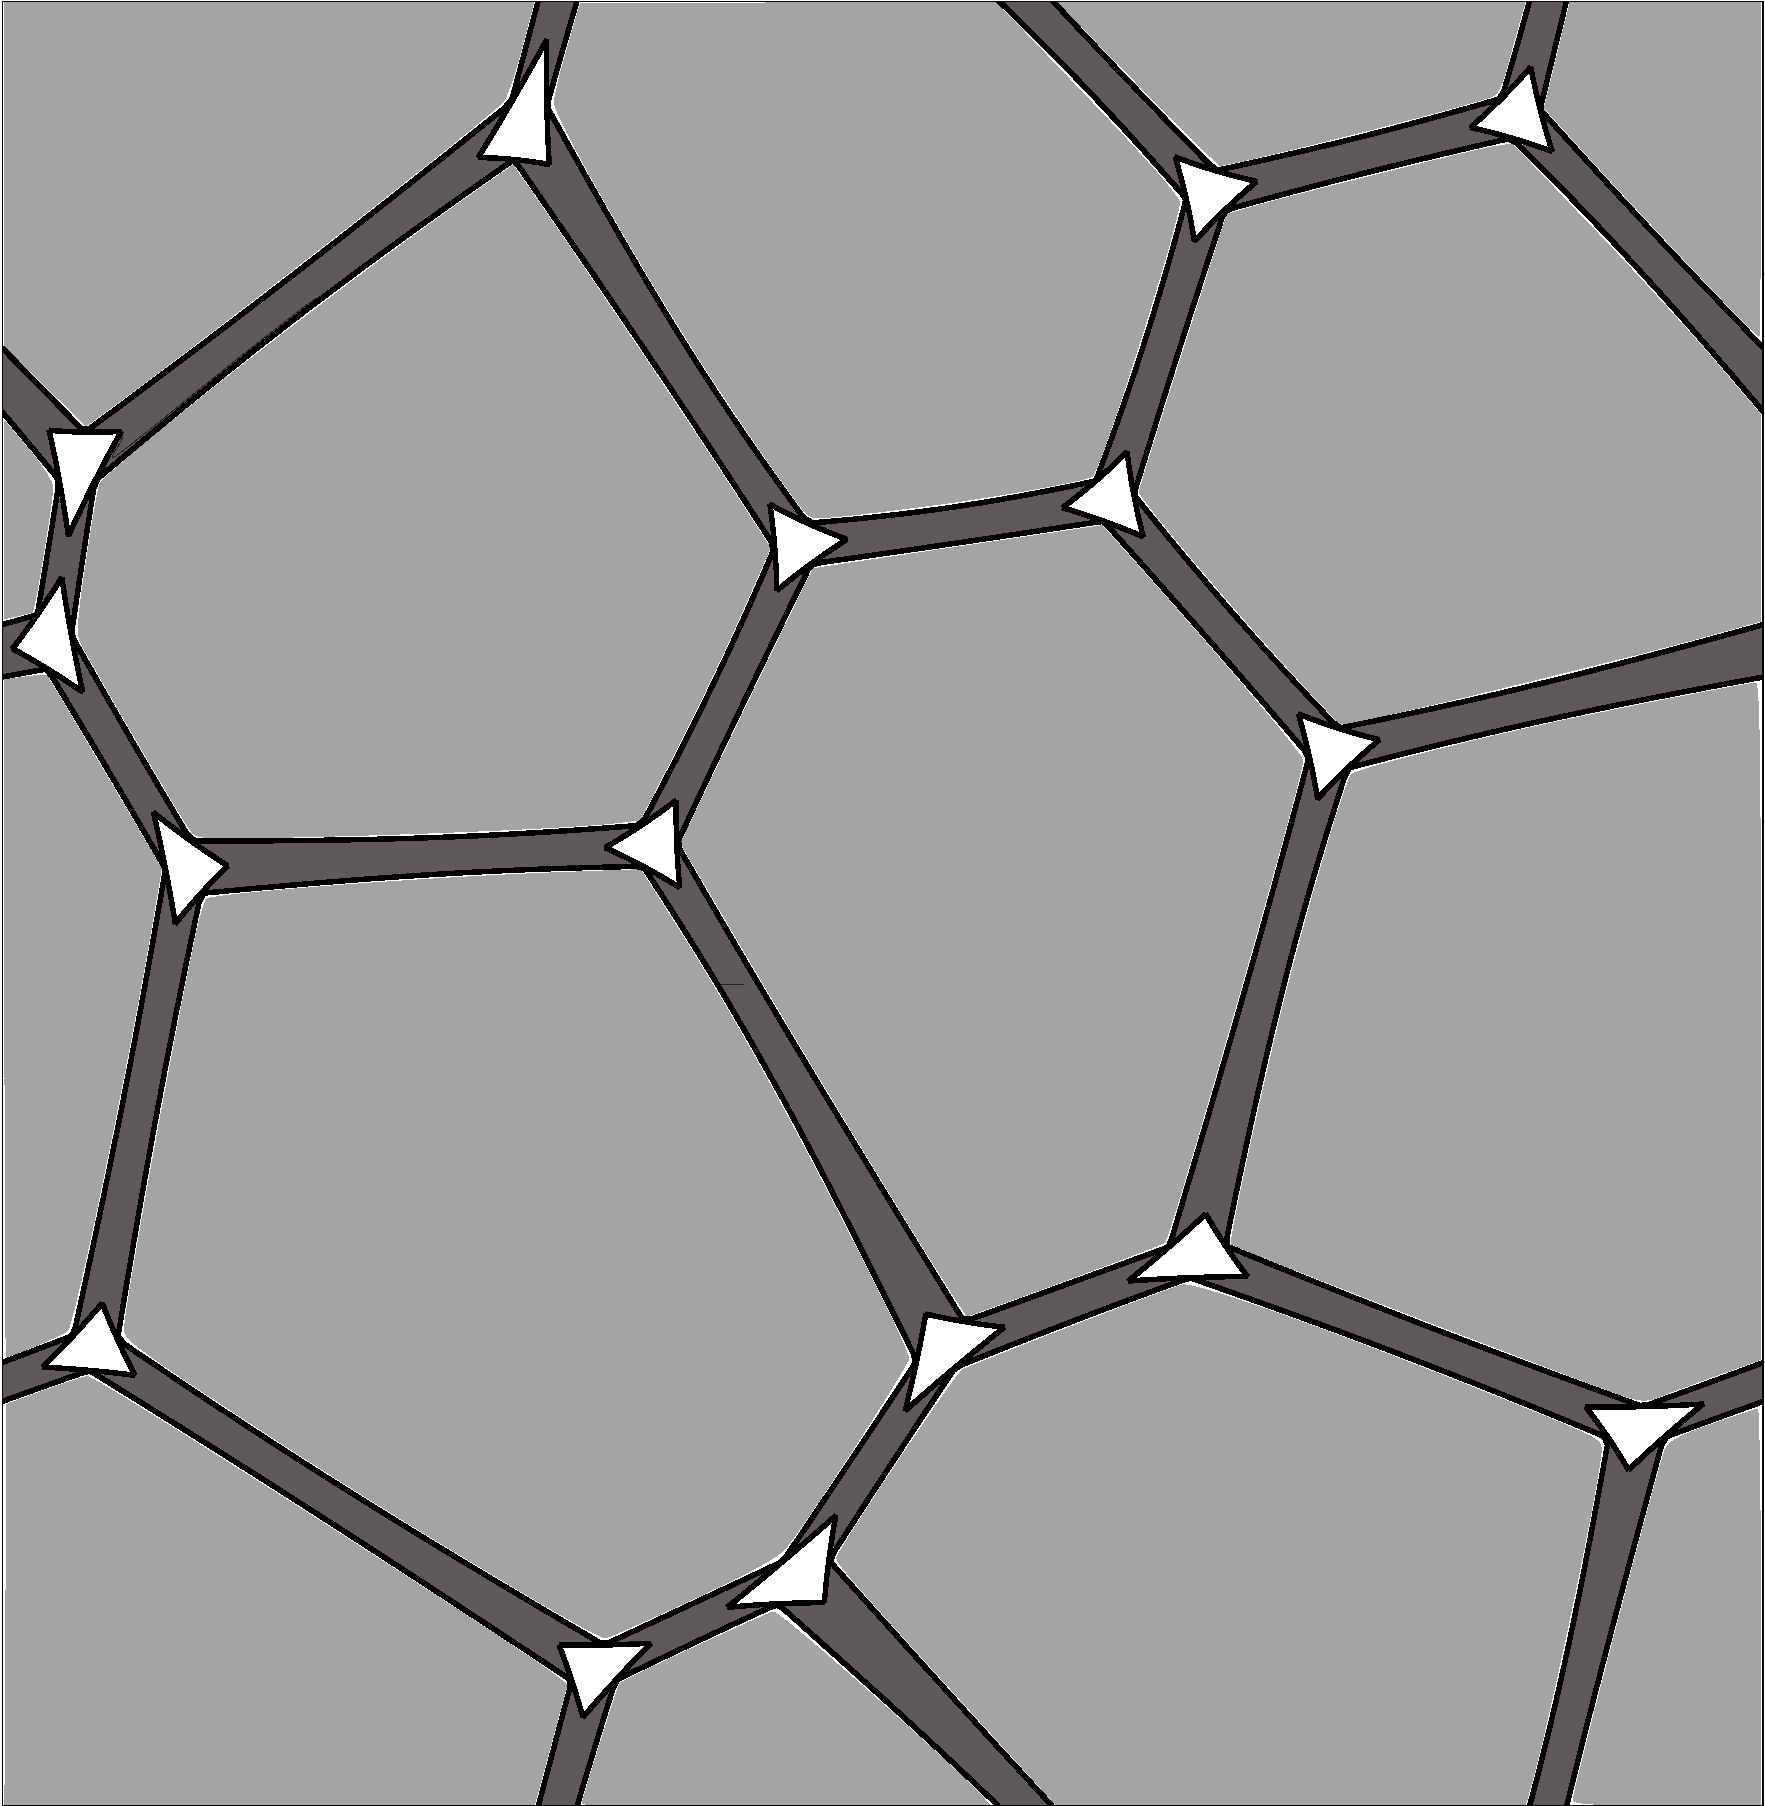
\includegraphics[width=\textwidth]{OP_t}
		\caption{}\label{plateau1}
	\end{subfigure}
	\begin{subfigure}[b]{0.32\textwidth}	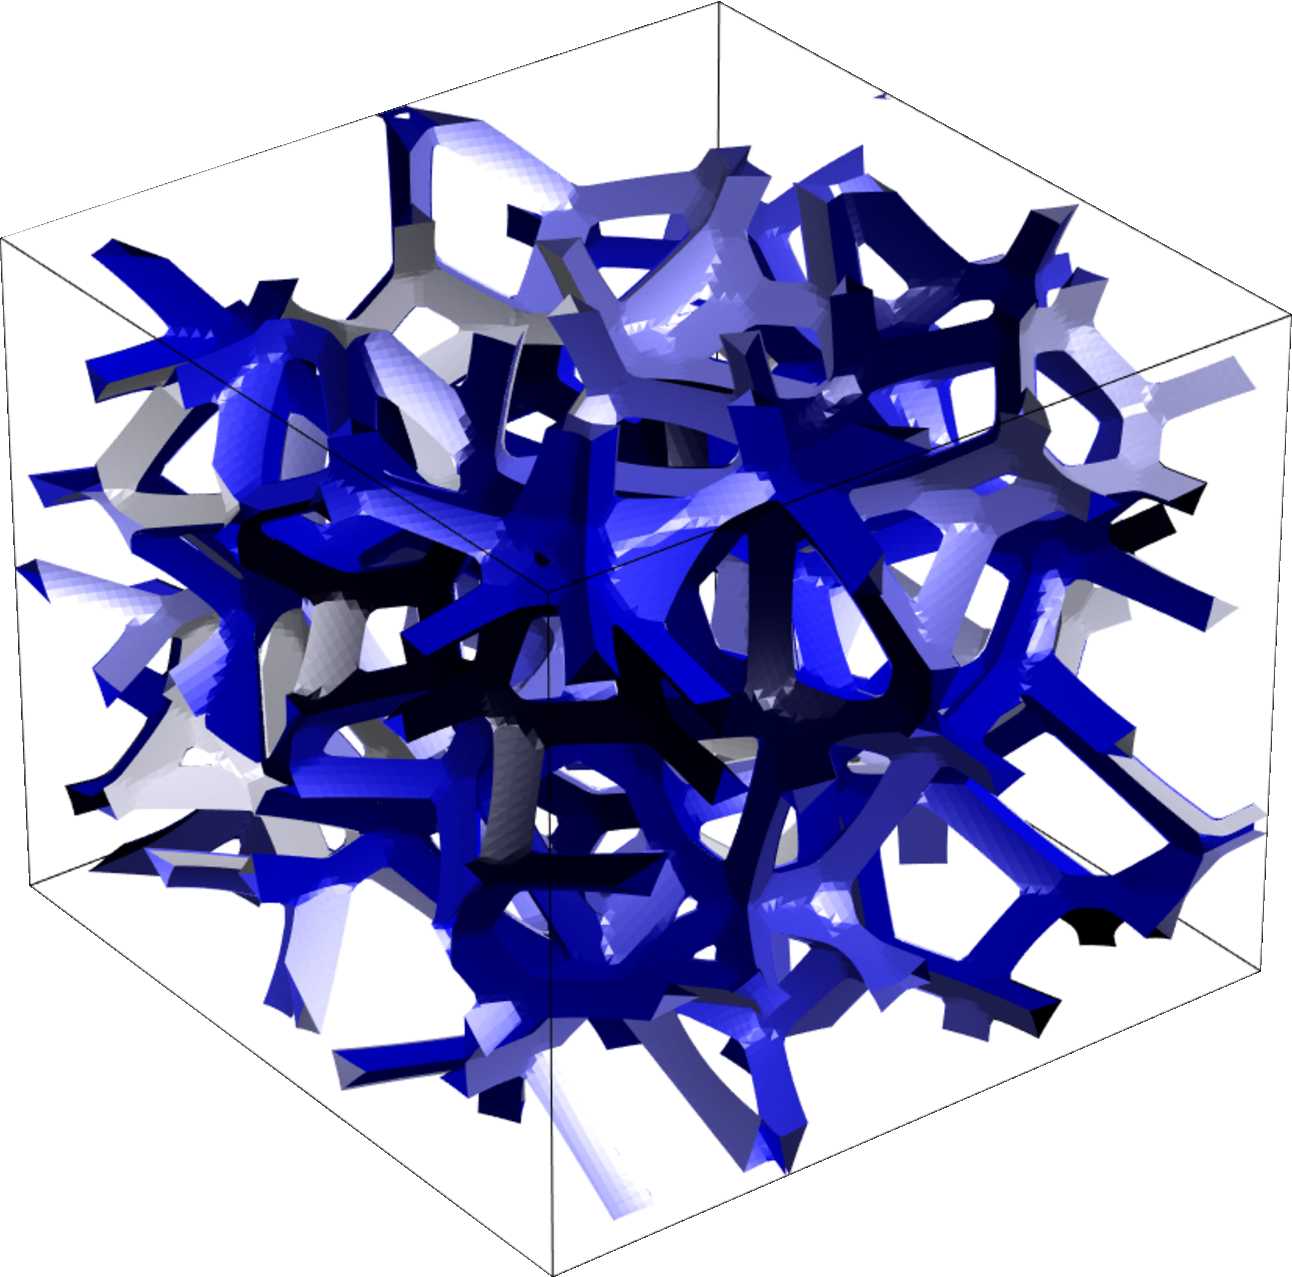
\includegraphics[width=\textwidth]{sharp_clean}
		\caption{}\label{plateau2}
	\end{subfigure}
	\caption{Plateau level set function; (a) with incremental $ t $ value, of 0.01 denoted by white line, 0.02 by black line, and 0.03 by dotted white line displaying the triangular nature of the isolines extracted by the function, and (b) illustration of the relation between the $ t $ level sets extracted from Eqs. (\ref{voronoi}) and (\ref{OP-2}); (c) Open foam extraction using Plateau level set functions  Eqs. (\ref{voronoi}) and (\ref{OP-2}) with $ t=0.15 $.}
\end{figure}

Figure \ref{plateau2} illustrates the example of an RVE in 3D extracted using the above relations.

\section{Morphology reconstruction from experimental CT-scans}\label{of-CT}
\sectionmark{Morphology reconstruction - CT-scans}

An approach to model foam structures based on the computation of the equilibrium micro-structure of soap froth was presented in \cite{jangMicrostructureOpencellFoams2008} using Brakke's Surface Evolver software \cite{brakkeMinimalSurfacesCorners1992,kraynikStructureRandomMonodisperse2003}. The tool starts with a random packing of spheres and uses the principle of minimization of surface energy that shapes the ``liquid'' into Plateau borders. The resulting structure is a periodic and isotropic RVE with a Gaussian-like strut length distribution. Such a process requires an important computational effort, as a large number of facets are required to discretize the Plateau borders. Also, the skeletal or a stick-figure model is extracted and the ligaments are simply modeled as shear deformable beams with the cross-section geometry based on the measured area distribution of the foam sample. This requires a further material volume correction at the nodes of the ligaments to account for excess material due to beam overlap. It was shown that extracting the seed points of a possible Laguerre tessellation based on the intersection nodes of a given foam sample produces tessellations that are similar in terms of morphological properties with those of simulated foams generated using Surface Evolver \cite{liebscherLaguerreApproximationRandom2015}.

In the previous section, the morphology extraction has been explained with the help of random spherical inclusion packings. The DN-RSA algorithm however is capable of generating any arbitrary shaped inclusion package, including ellipsoids and polyhedrals among the various types of inclusions that are present in the wide range of materials that are used in general day-to-day activities, while simultaneously updating the associated distance fields to the respective inclusions. This tool can be modified to completely skip the RSA part, and use any set of pre-conceived inclusion packing and assign the respective distance fields. In \cite{leblancAnalysisOpenFoamUnderPreparation}, the authors propose a methodology to reconstruct an open foam morphology from computerized tomography (CT) scans. One can extract the basis geometries as implicit expressions of the respective polyhedrals. A distance field from these geometries can then be generated using the tools explained in \cite{ehabmoustafakamelIntegratedApproachConformal2019} which can then be used instead of $ O_P(\textbf{x}) $ of Eq. (\ref{OP}). In this context, the modified tool can be called DN-CT-SCAN. In a similar manner, a modified tool based on distance fields has been used to study CT-scans of composites in \cite{wintibaAutomatedReconstructionConformal2020}. In this section, tools necessary to reconstruct morphologies of the open foam geometries from CT-scans are discussed and the functions required to optimize the geometries are presented.

\subsection{Image analysis}\label{of-CT-image}
To extract the morphology, the geometric characteristics need to be extracted from a CT scan image of the material. Due to the coarse resolution of such images, a straight forward approach to binarize and label the image can not be applied and requires in general a chain of processing algorithms\cite{lautensackFittingThreedimensionalLaguerre2008}. This process can be summarized as follows:
\begin{itemize}
	\item Application of simple threshold on the material system for image segmentation;
	\item Application of the Euclidean distance transform on the resultant black-and-white image. This results in the formation of a distance field to each background pixel that describes the distance to the nearest strut;
	\item Application of filters and morphological transforms to remove superfluous local maxima created during the distance field extraction, like h-maxima transform\cite{jierongchengSegmentationClusteredNuclei2009,schladitzGeometricCharacterisationLight2006} or grey-scale reconstruction\cite{vincentMorphologicalGrayscaleReconstruction1993};
	\item Application of the watershed algorithm\cite{vincentWatershedsDigitalSpaces1991} to convert the distance fields into cells.
\end{itemize}

In \cite{leblancAnalysisOpenFoamUnderPreparation}, the authors have presented an alternative to the watershed algorithm by using an inclusion clustering based method. In this method, standard inclusion shapes like ellipsoids are allowed to grow and cluster together using a computationally cheap algorithm. An iterative process is used to construct ellipsoids by allowing them to grow inside associated polyhedrals that are defined by the local maxima, including the superfluous ellipsoids. This can be achieved by an optimization procedure, like the iterative regional inflation by semi-definite programming, or IRIS \cite{deitsComputingLargeConvex2015}. This process is similar to that of the growth of Voronoi or Laguerre tessellation. The added benefit of the ellipsoid based packing is that the anisotropy in the material sample is implicitly captured by ellipsoids and such models have generally been found to be more precise than the ones developed from spherical packings \cite{teferraTessellationGrowthModels2015,sedivy3DReconstructionGrains2016}.

Once the ellipsoids are generated, a clustering algorithm, like the generalized density based scan (GDBScan)\cite{sanderDensityBasedClusteringSpatial1998}, can be used to cluster intersecting ellipsoids based on their relative intersecting volume. Using a merging algorithm, like the Minimum Volume Covering Ellipsoids of Ellipsoids (MVCEE)\cite{yildirimMinimumVolumeCovering2006}, the ellipsoids recognized to be part of the same cluster are merged. These ellipsoids can be then used as the basis for DN-CT-SCAN, and the further process of extracting the distance neighbors and distance fields can be carried out as described previously to extract the variational strut geometry (Figure \ref{fig-of-ellipsoids}).

The ellipsoids generated this way are based on reference polyhedrals. In fact, by utilizing a normal vector, the polyhedral faces can be translated to ensure that the resulting union of polyhedrals comply with the density of the foam sample which is used as the target foam in the reconstruction process\cite{leblancAnalysisOpenFoamUnderPreparation}. Considering the versatility of DN-CT-SCAN method, the developed polyhedrals can also be used as the base inclusions to generate an inclusion packing to develop an open foam morphology.

It needs to be mentioned here that the seed value of the ellipsoids used in DN-CT-SCAN can also be used as the seed value in the DN-RSA algorithm, to generate spherical packing where a maximum sphere radius can be ensured so that no two generated spheres are intersecting. However, this study will be limited to the morphologies extracted based on ellipsoids and polyhedrals only, considering that these geometries are already a close approximation of the actual physical foam sample from which the geometries have been derived. Further description on the methodology used and its implementation can be found in \cite{leblancAnalysisOpenFoamUnderPreparation}.

Once the explicit geometries of the ellipsoids and polyhedrals are obtained in the form of a conformal triangulation (Figure \ref{fig-of-polyhedra}), an implicit description of the geometries in terms of distance fields can be generated by using the methodology presented in \cite{ehabmoustafakamelIntegratedApproachConformal2019} so that the distance field can be used in the various post processing techniques explained in the following sections.

\begin{figure}
	\centering
	\begin{subfigure}{0.45\textwidth}
		\includegraphics[width=\textwidth]{CT_scans}
		\caption{}
	\end{subfigure}
	\begin{subfigure}{0.45\textwidth}
	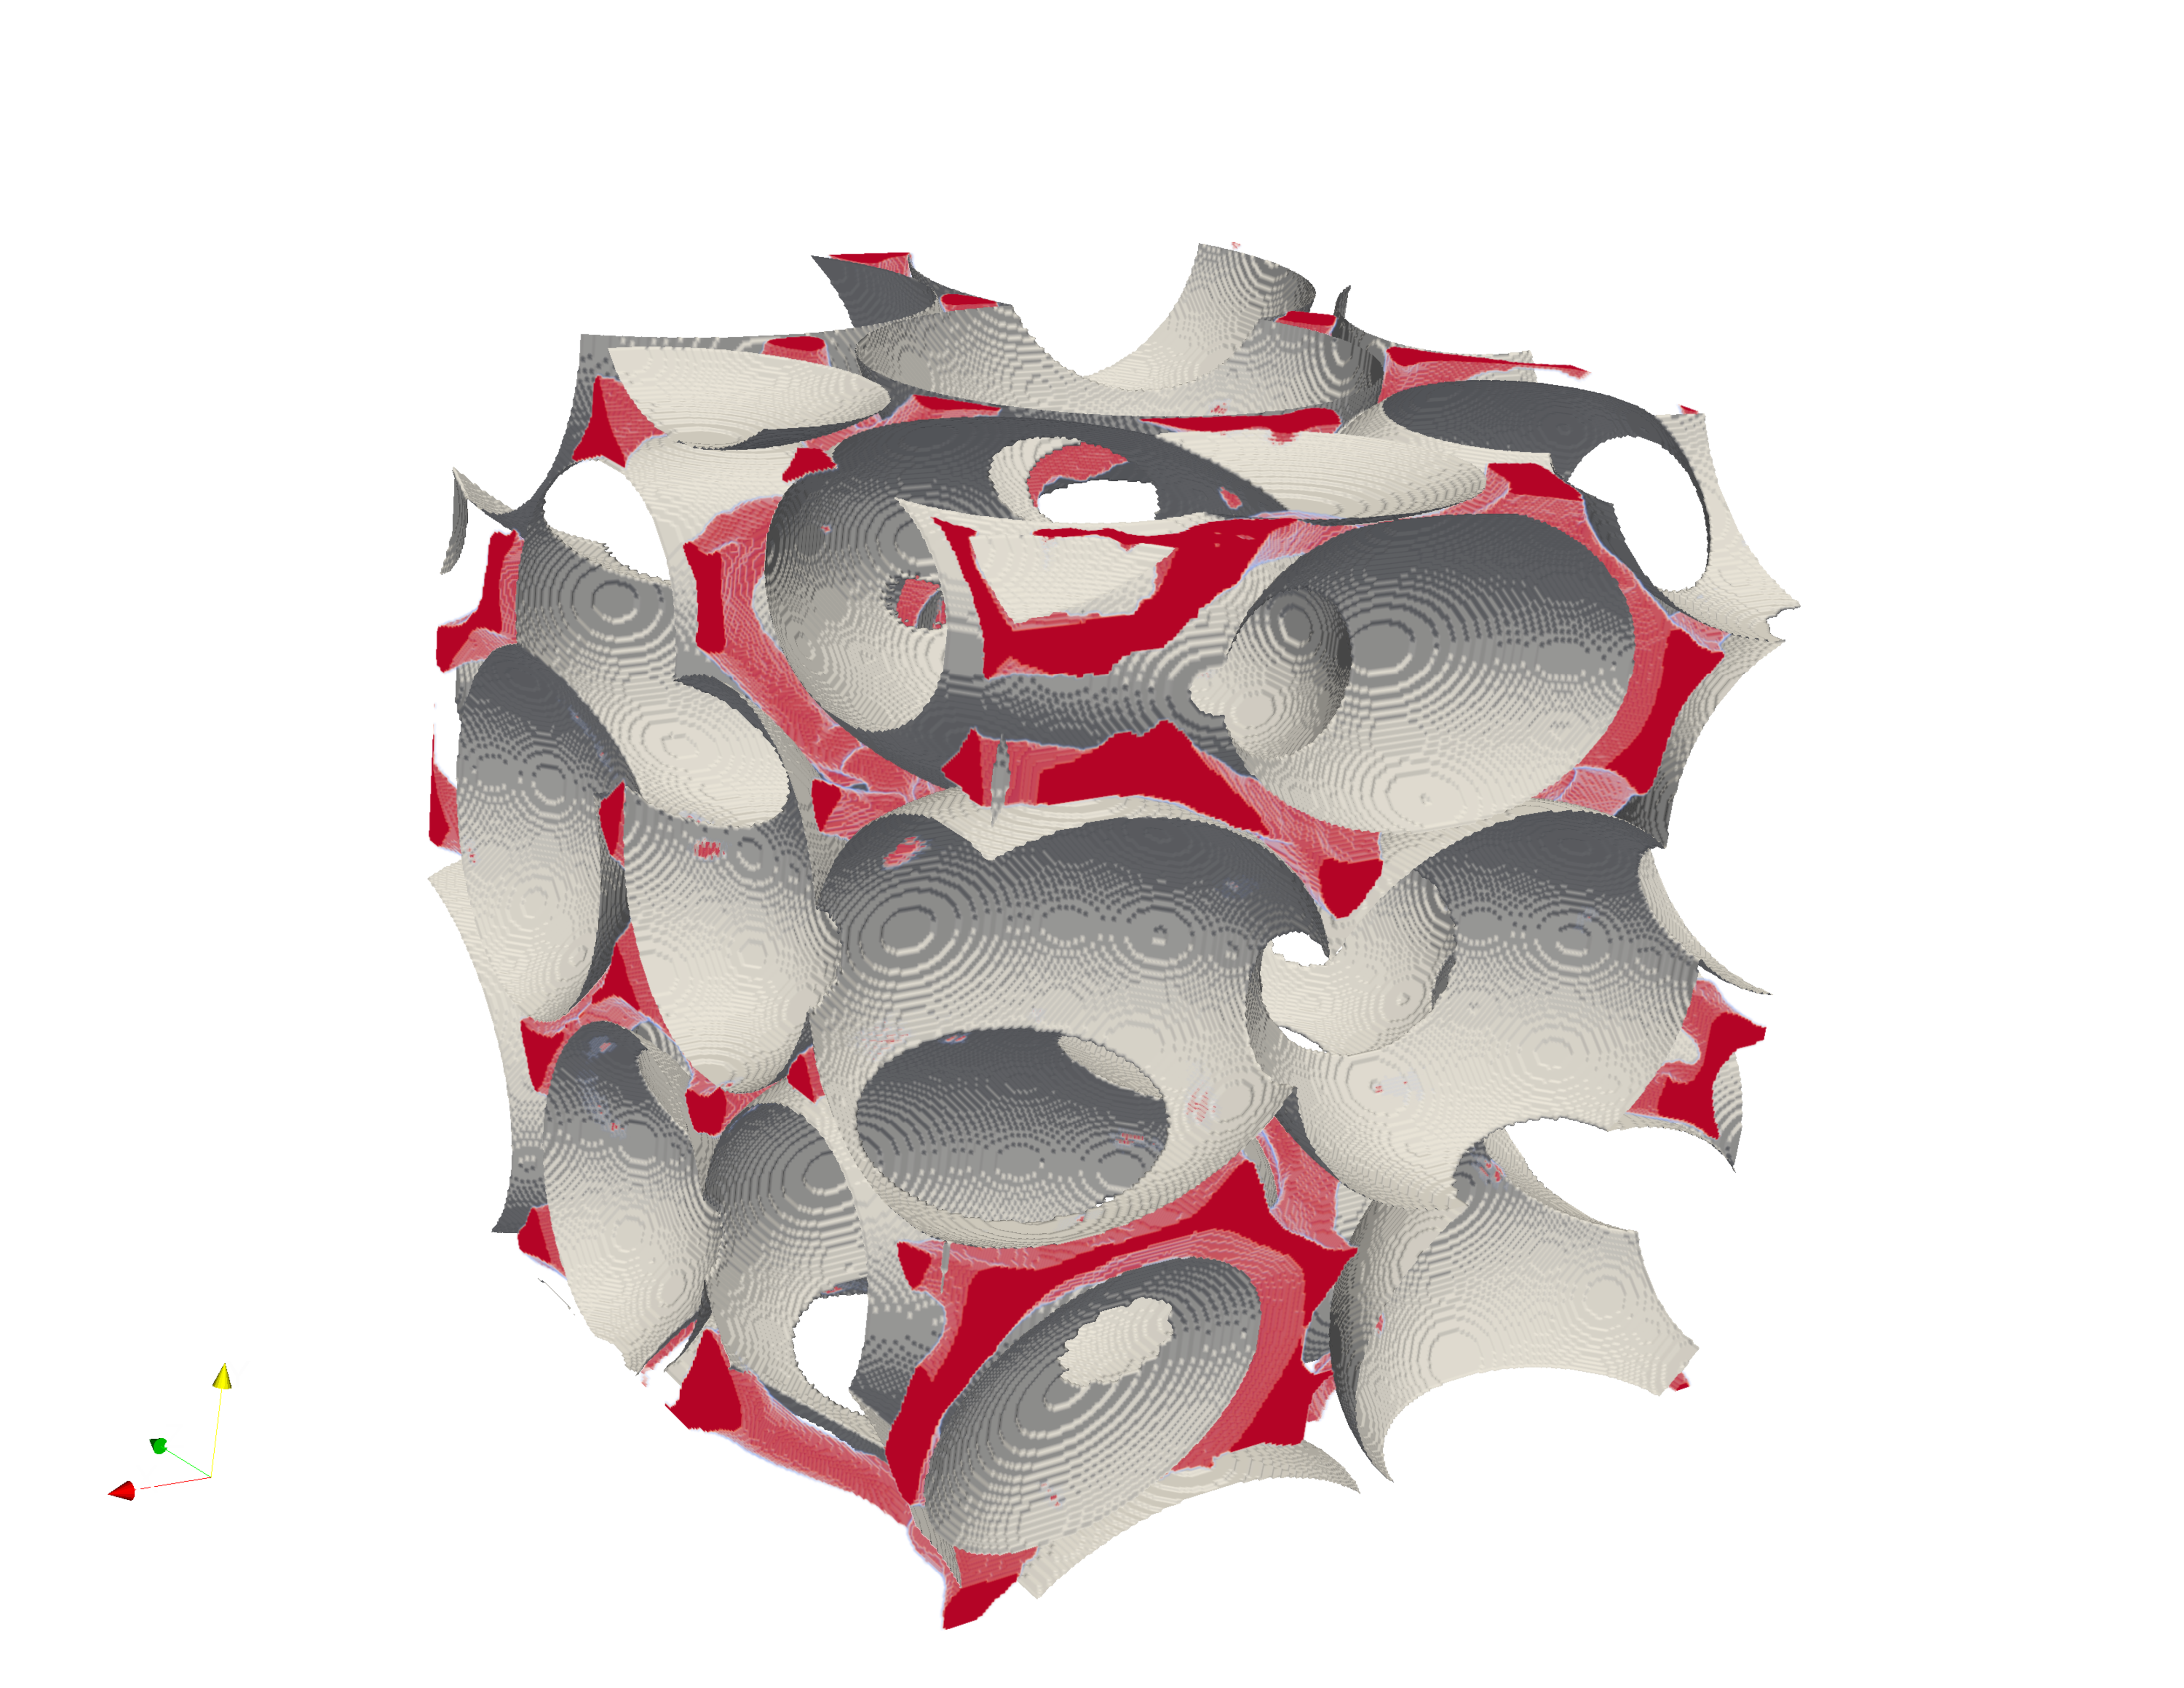
\includegraphics[width=\textwidth]{ct_ellispoid}
		\caption{}
	\end{subfigure}
	\caption{(a) Voxels obtained from CT-scans of physical foam samples\cite{jungMicrostructuralCharacterisationExperimental2017}; (b) Extracted ellipsoids embedded in the voxel data\cite{leblancAnalysisOpenFoamUnderPreparation}.}\label{fig-of-ellipsoids}
\end{figure}

\begin{figure}
	\centering
	\begin{subfigure}{0.45\textwidth}
		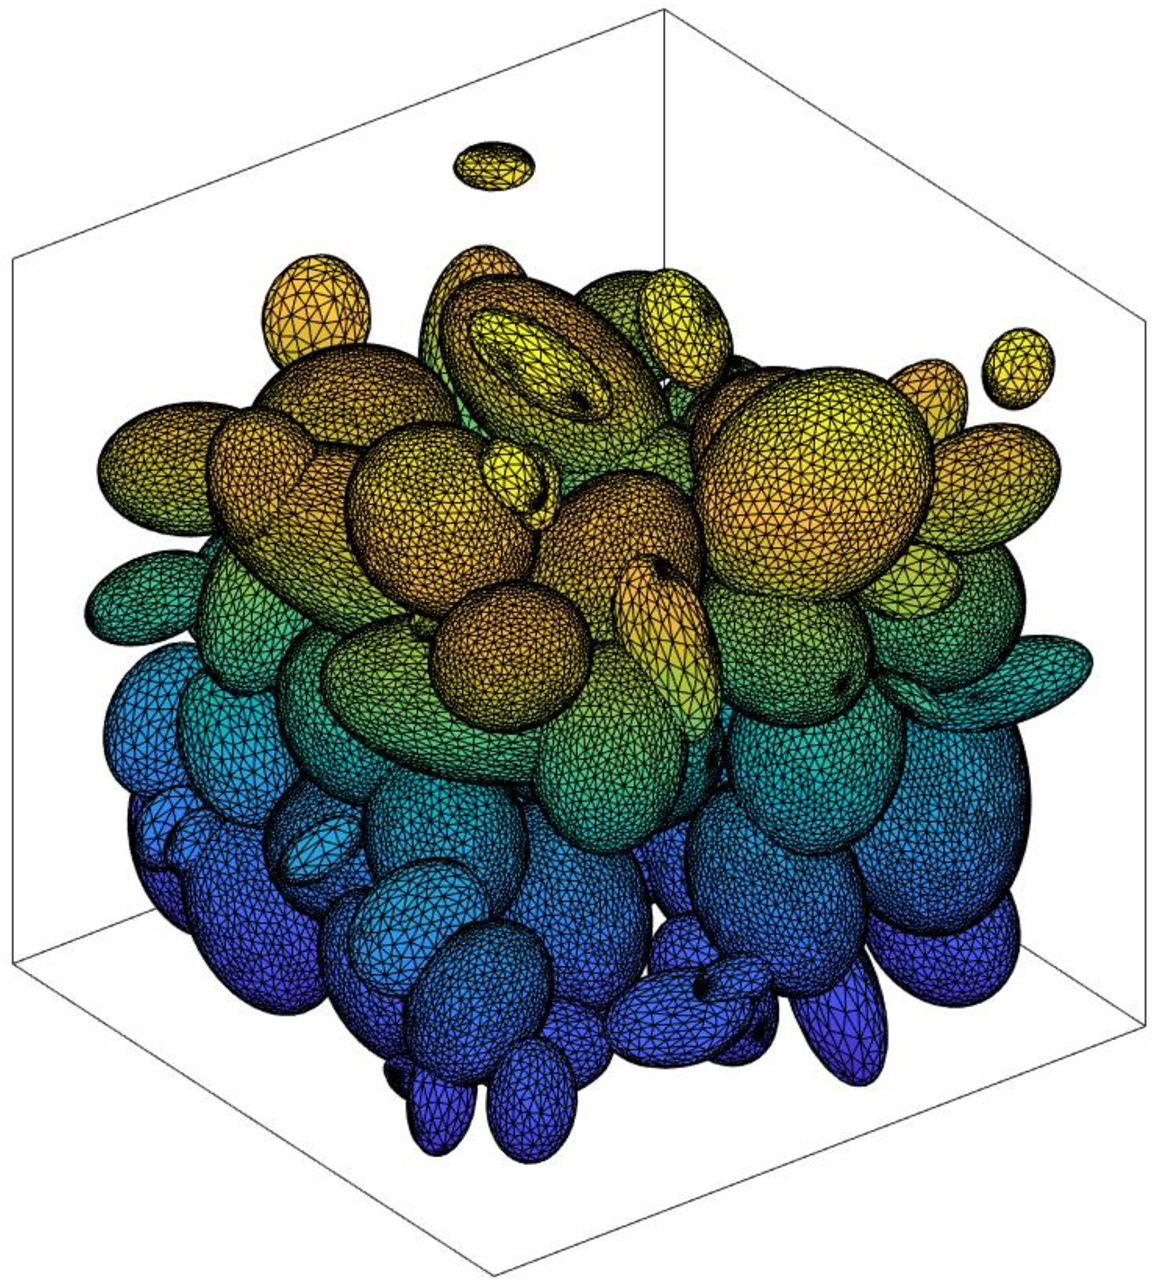
\includegraphics[width=\textwidth]{ellipsoids}
		\caption{}
	\end{subfigure}
	\begin{subfigure}{0.45\textwidth}
		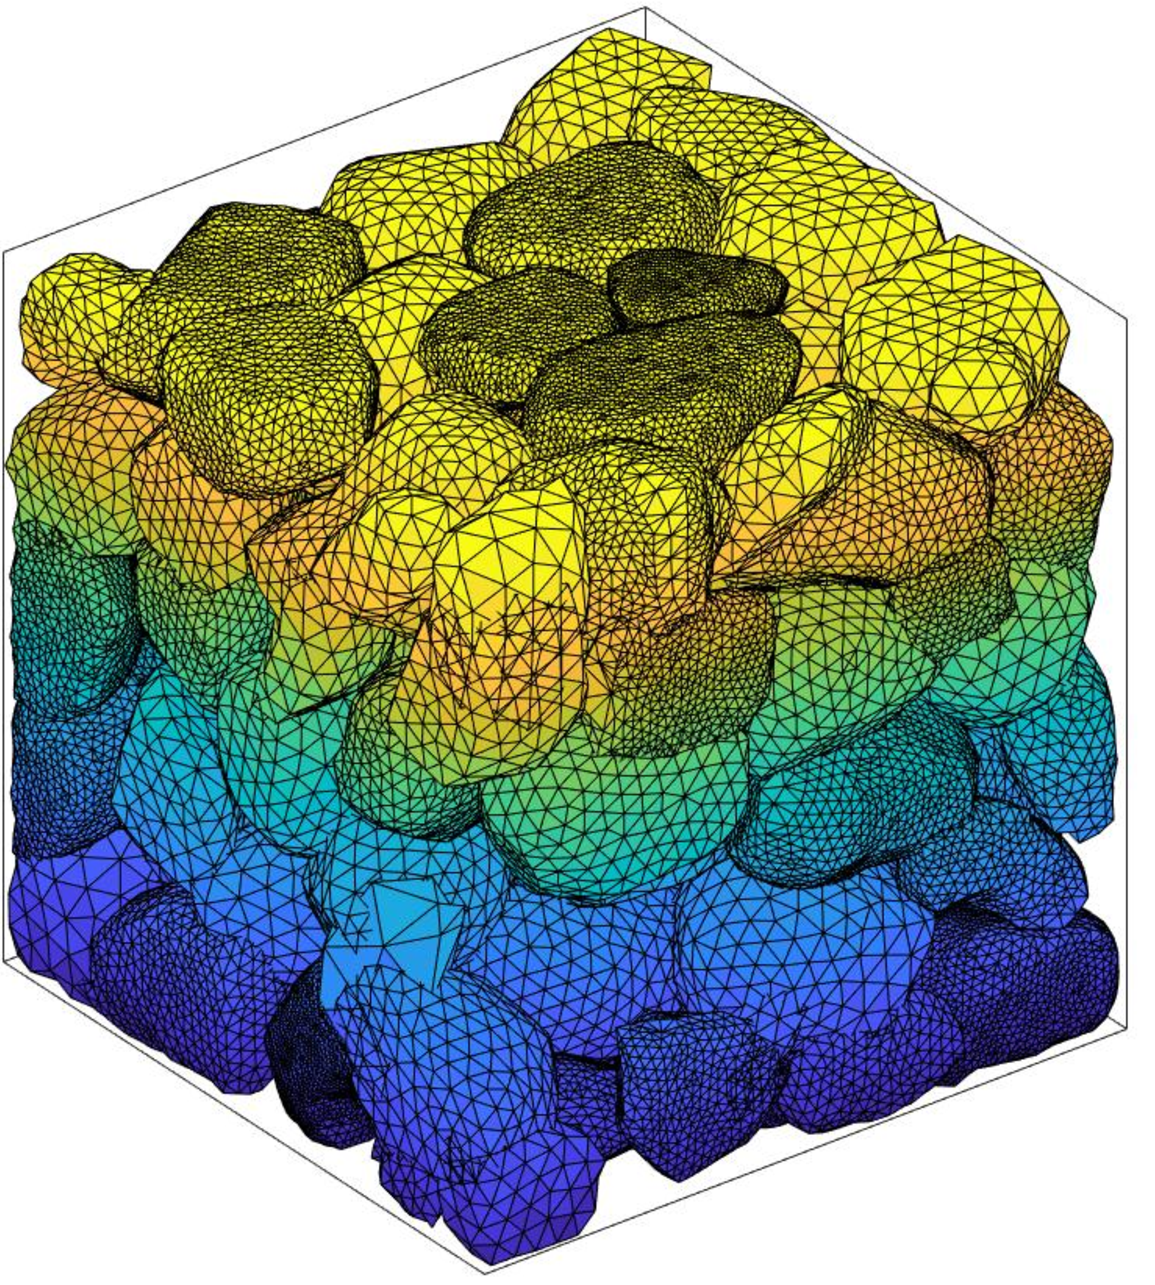
\includegraphics[width=\textwidth]{polyhedrals}
		\caption{}
	\end{subfigure}
	\caption{(a) Extracted ellipsoids and (b) the corresponding polyhedrals from CT-scan voxels.\cite{leblancAnalysisOpenFoamUnderPreparation}.}\label{fig-of-polyhedra}
\end{figure}

\subsection{Inclusion treatment}\label{of-CT-incl}

\begin{figure}
	\centering
	\begin{subfigure}[p]{\textwidth}
		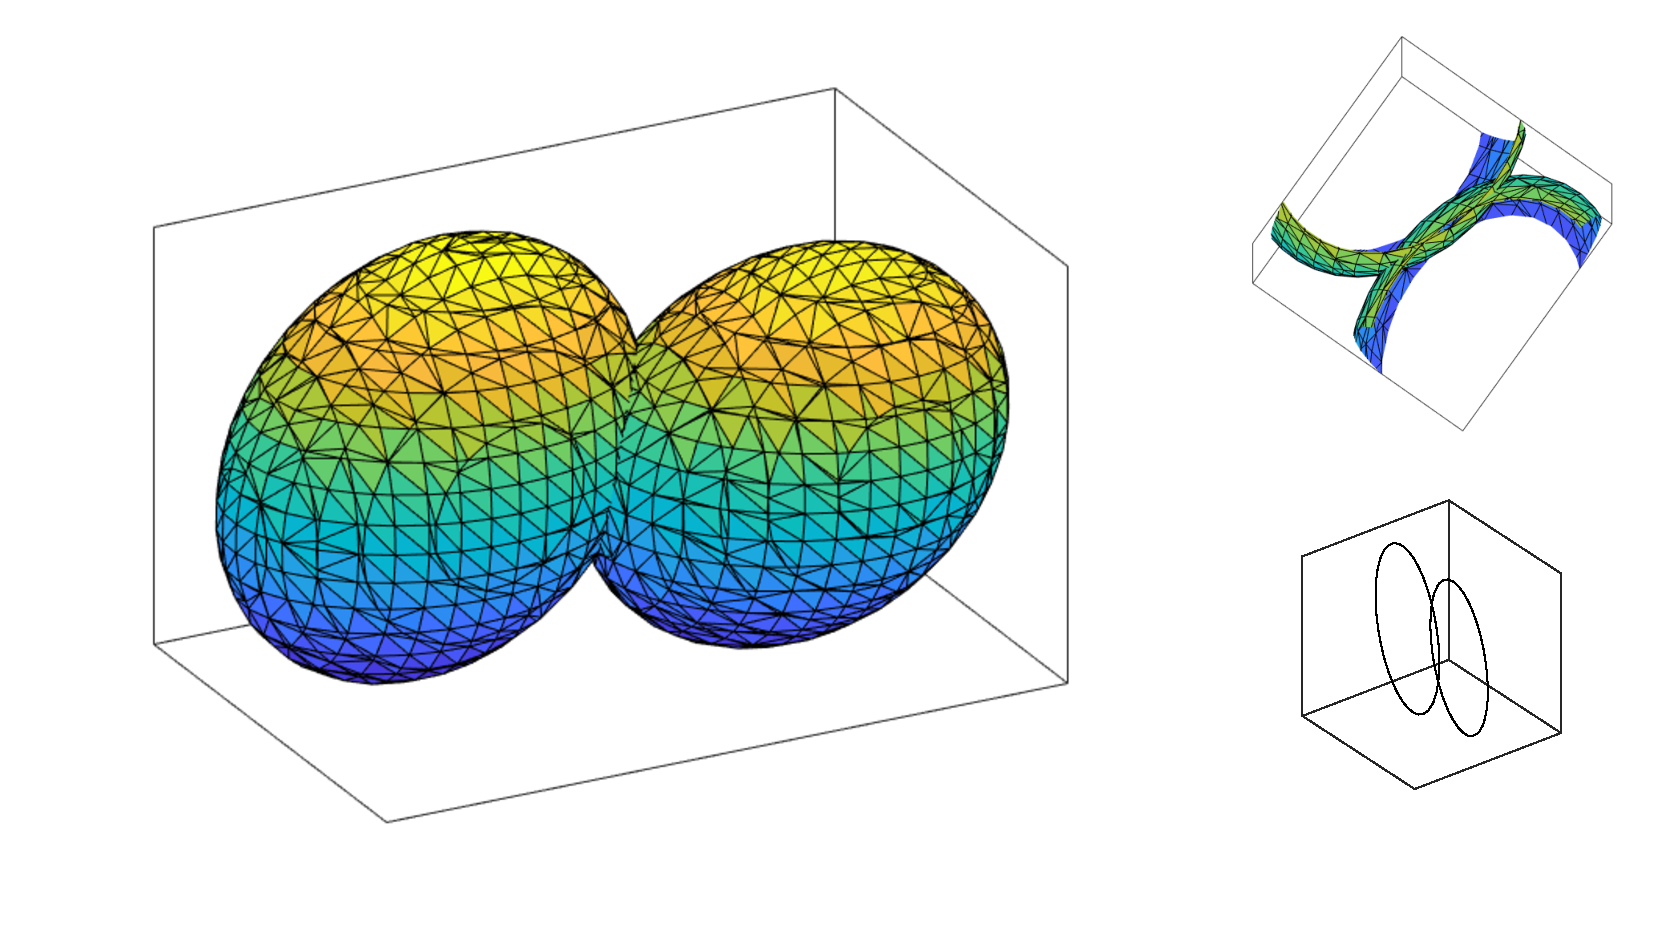
\includegraphics[height=7cm]{ellipsoid_interpenetration_2}
		\caption{}
	\end{subfigure}
	\begin{subfigure}[p]{0.3\textwidth}
		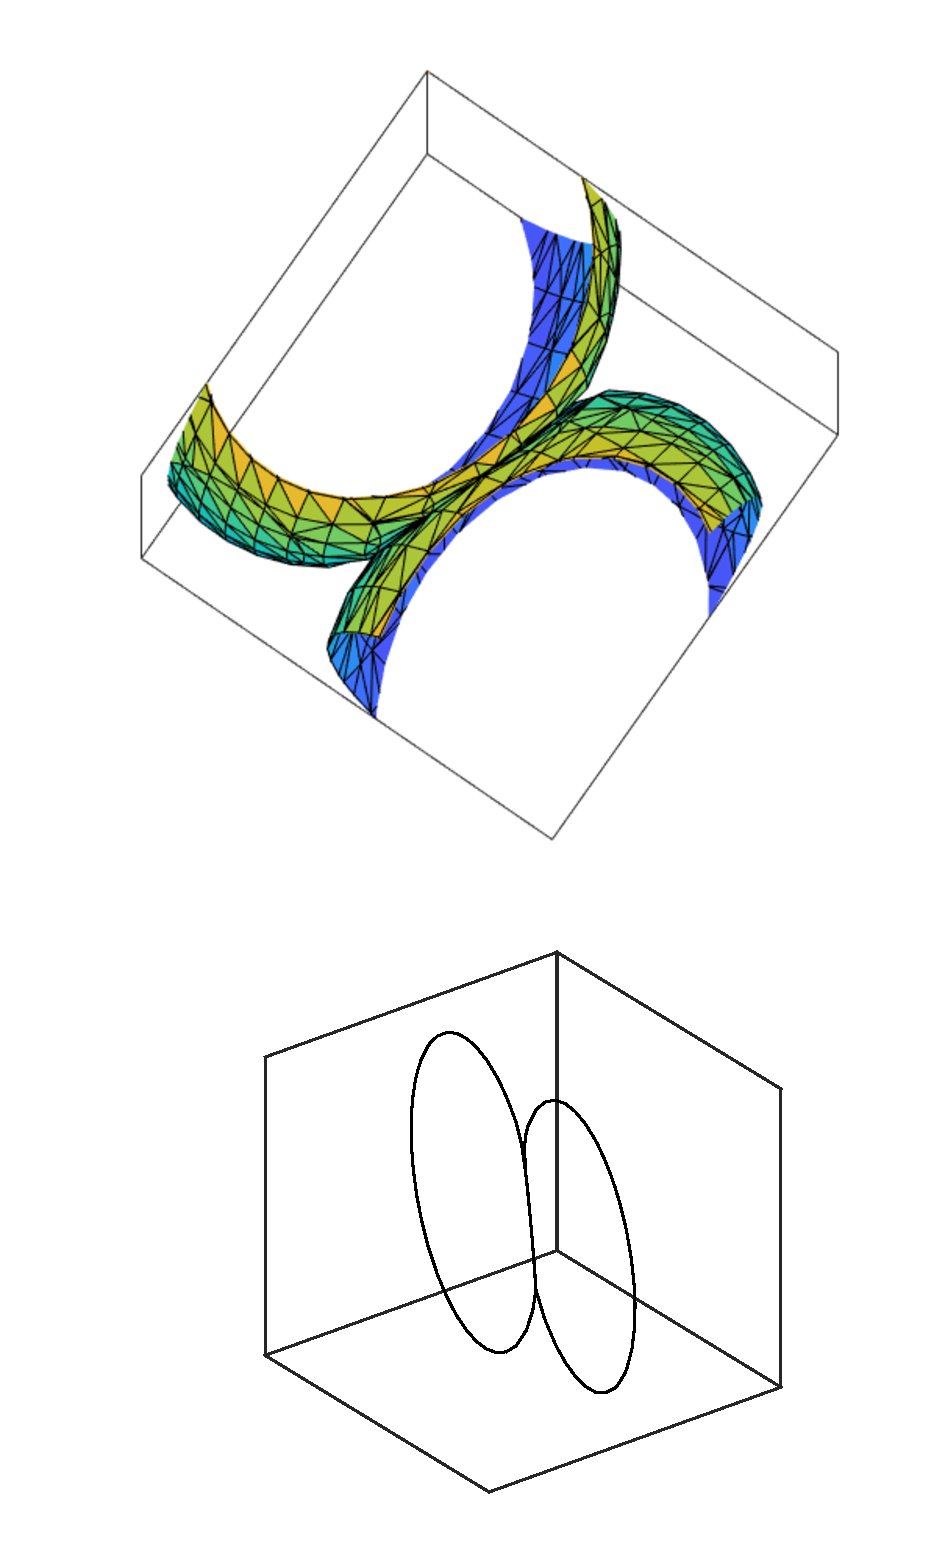
\includegraphics[height=7cm]{ellipsoid_interpenetration_no_gap2}
		\caption{}
	\end{subfigure}
	\begin{subfigure}[p]{0.6\textwidth}
		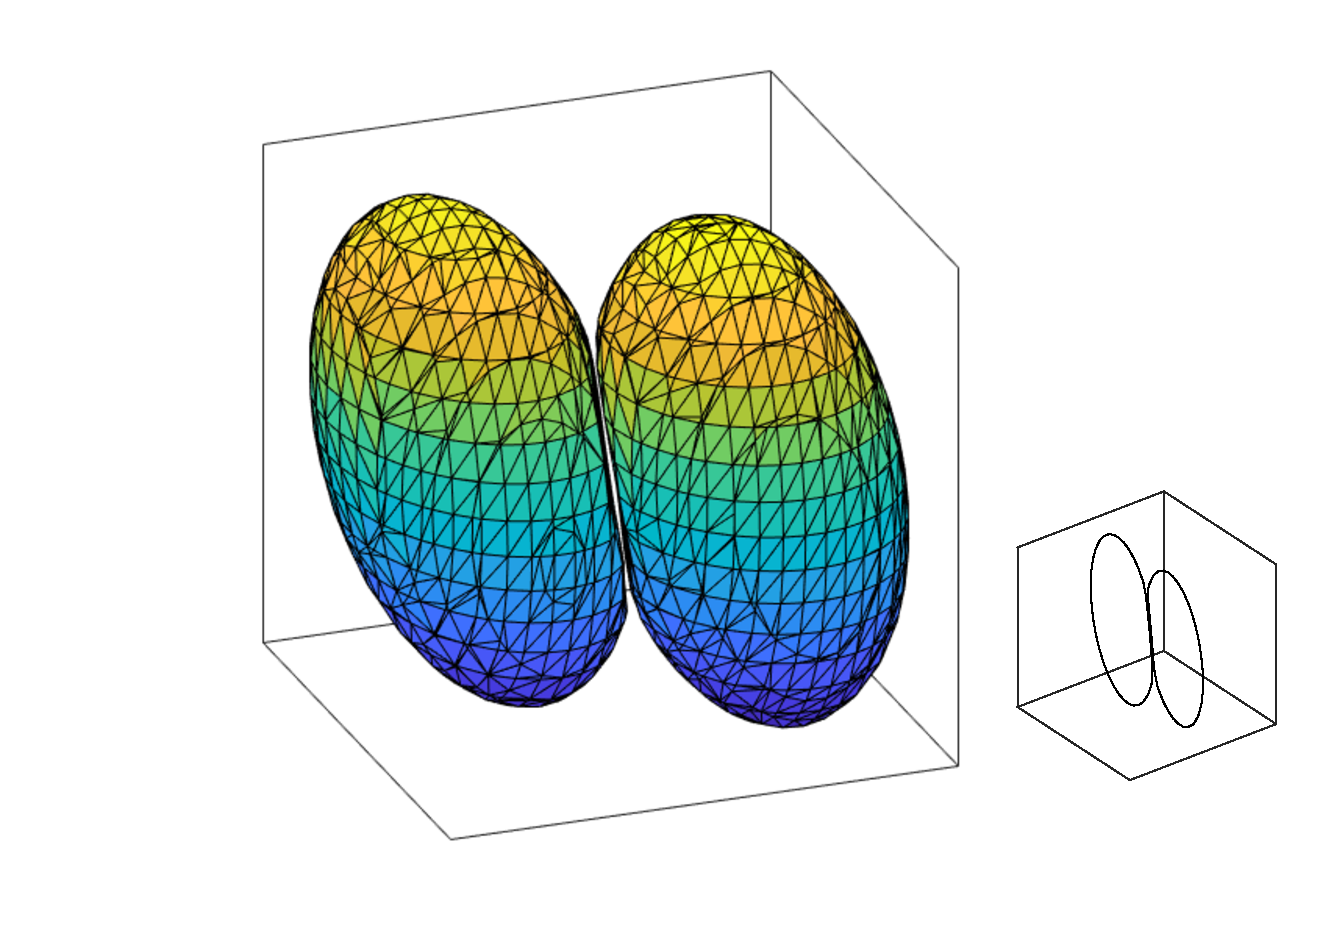
\includegraphics[height=7cm]{ellipsoid_no_interpenetration_2}
		\caption{}
	\end{subfigure}
	\caption{(a) Ellipsoids obtained by processing the CT-scan, the interpenetration can be seen by the sectional plot; (b) Post-processing of ellipsoids to avoid residual inter-penetrations, the ellipsoids now share a common face; (c) Ellipsoids after post-processing and introduction of a gap, the ellipsoids no longer share a common face}\label{fig-interpenetrations}
\end{figure}

\begin{figure}
	\centering
	\begin{subfigure}[b]{0.45\textwidth}
		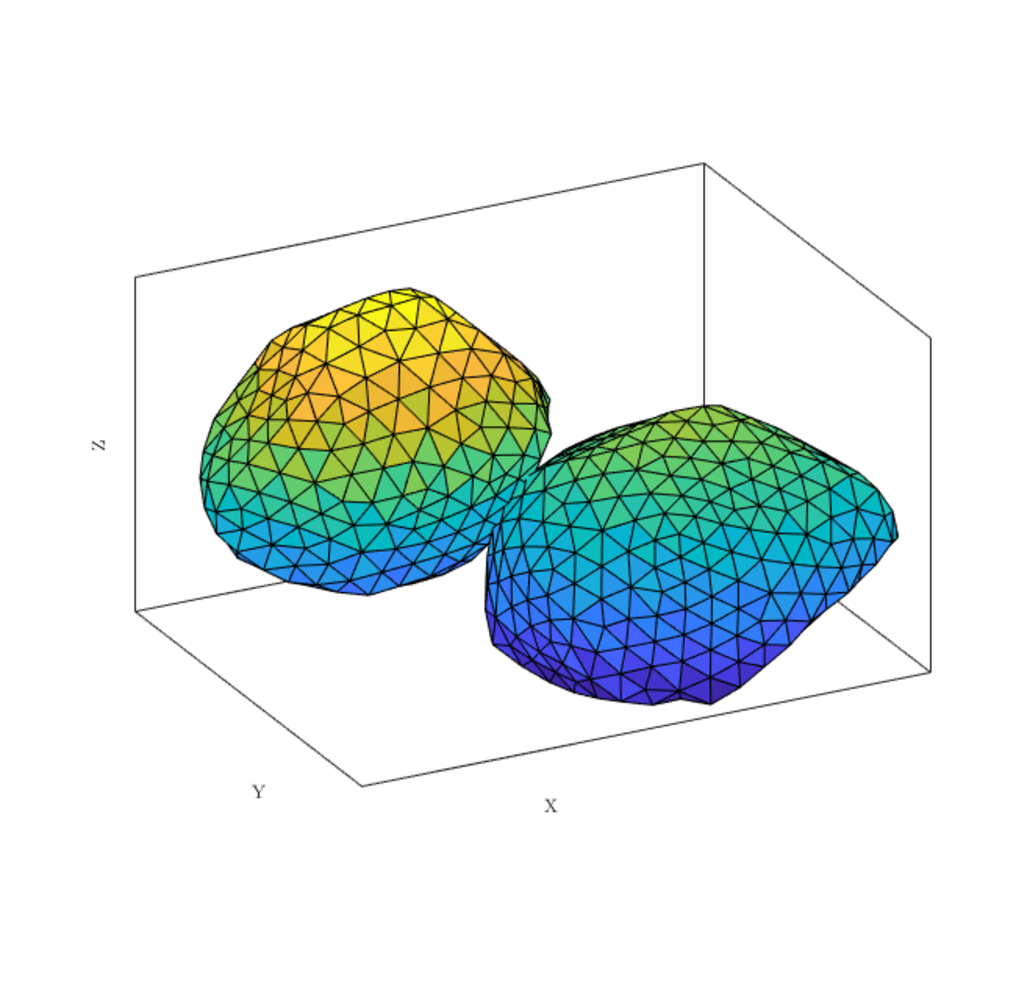
\includegraphics[width=\textwidth]{polyhedra_intersection}
		\caption{}
	\end{subfigure}
	\begin{subfigure}[b]{0.45\textwidth}
		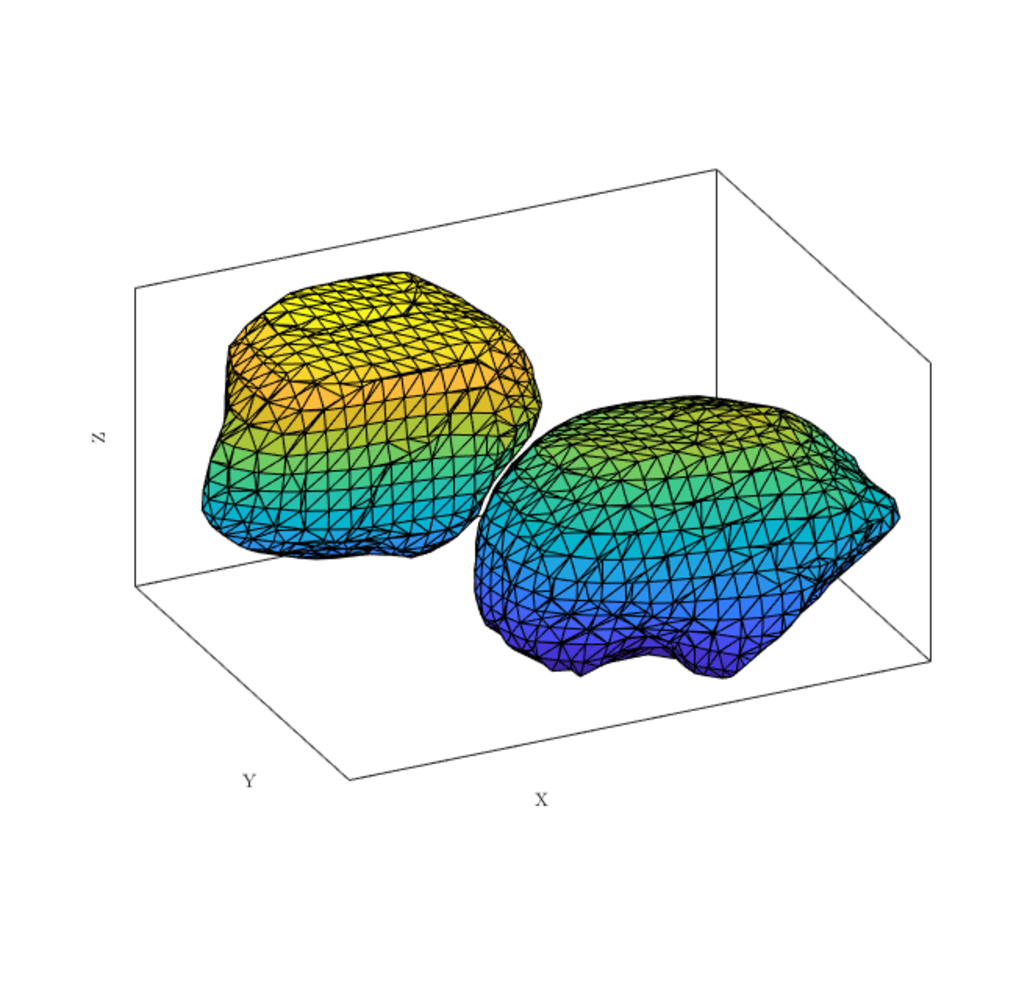
\includegraphics[width=\textwidth]{polyhedra_intersection_post}
		\caption{}
	\end{subfigure}
	\caption{(a) Polyhedrals after image processing; (b) Polyhedrals after post processing and introduction of a gap.}\label{fig-interpenetrations-poly}
\end{figure}

The generated inclusions are prone to a high degree of interpenetration and face sharing. In the case of ellipsoids, a large number of inclusions have mutual intersections that would pose a problem of appropriate generation of the signed distance function used to assign the appropriate distance neighbor. In the case of polyhedrals, all polyhedrals end up sharing faces with each other and this could create problems in the ideal recognition of the correct neighbor leading to spurious distance neighbor parameters (Figures \ref{fig-interpenetrations}(a) and \ref{fig-interpenetrations-poly}(a)).

To avoid the confusions related to identifying the correct neighbors, these interpenetrations need to be treated accordingly. An easy way to proceed with this treatment is to introduce a general minimal offset in all the inclusions to ensure that the inclusions do not intersect anymore\cite{sononLevelSetBasedRepresentative2013}. In \cite{wintibaAutomatedProcedureGeneration2017}, the DN-RSA tool has been applied in the context of individual yarns of textile reinforced composites to remove residual inter-penetrations. The same methodology can be applied in the context of inclusions generated by reconstructing the morphology and implemented in DN-CT-SCAN. This study is quite close in concept to one presented in \cite{wintibaAutomatedReconstructionConformal2020} where the CT-scan images is used to reconstruct composite structures using distance fields. The intersection volume between two inclusions can be determined as 
\begin{equation}\label{eq-of-pene1}
\text{max}(DS_i(\textbf{x}),DS_j(\textbf{x}))<0,\quad\forall i\ne j.
\end{equation}
By considering the minimal distance to all inclusions except inclusion $ i $ as $ DO_i(\textbf{x}) $,
\begin{equation}\label{eq-of-pene2}
DO_i(\textbf{x})=\text{min}(DS_j(\textbf{x})),\quad\forall i\ne j,
\end{equation}
an ad-hoc level set function $ O_i(\textbf{x}) $ can be extracted, such that
\begin{equation}\label{eq-of-pene3}
O_i(\textbf{x})=\text{max}(DS_i(\textbf{x}),(DS_i(\textbf{x})-DO_i(\textbf{x}))).
\end{equation}

The contour of the above function gives the surface of the modified ellipsoids in contact, which is shown in Figure \ref{fig-interpenetrations}(b). In addition to obtaining the contact surface, a gap can be introduced between the ellipsoids in contact. This is particularly useful in the case of numerical modeling, to ensure that the discrete space can identify the corresponding neighbor accurately. This gap can be introduced as an offset\cite{sononLevelSetBasedRepresentative2013}, $ c $, and the zero level of such a contour can be extracted by the function
\begin{equation}\label{eq-of-pene4}
O_i^g(\textbf{x})=\text{max}(DS_i(\textbf{x}),(DS_i(\textbf{x})-DO_i(\textbf{x}))+c).
\end{equation}
The contours of $ O_i^g(\textbf{x}) $ gives the surface of the modified ellipsoids as shown in Figure \ref{fig-interpenetrations}(c) and for modified polyhedrals as shown in Figure \ref{fig-interpenetrations-poly}(b).

The function $ O_i^g(\textbf{x}) $ is then used instead of $ DS_i(\textbf{x}) $ and is used to refresh the previously stored distance functions $ DN_k $ and the neighbor identity map $ NN_k $ can be retrospectively updated. With these modified distance functions, the process for further development of open foam morphologies remains the same and can be used as is for the DN-RSA tool presented in Section \ref{of-gen}.

\section{Detailed foam morphology features}\label{of-feature}
Realistic features that are seen according to CT-scans in real foams can be introduced in RVEs with the help of functions built on the basis of the distance fields. The extraction of some of these characteristically important features in this section are based on the  suggestions provided in \cite{sononAdvancedTechniquesGeneration2014}, and an original methodology to extract complexities in strut geometry like the variation of strut cross-section is presented here. This methodology can be applied on the distance functions of either the random sphere-distributions obtained using the DN-RSA algorithm as presented in Section \ref{of-gen} or the inclusions extracted from CT-scan images using DN-CT-SCAN algorithm as presented in Section \ref{of-CT}.

\subsection{Open / close faces}\label{of-feature-open}
Observations from micro-CT have shown the existence of several sites in a metallic open cell foam where existing holes in the original polymeric template have been presumably filled in during the molding process (Figure \ref{open-close1})\cite{jangMicrostructureOpencellFoams2008}.  Such sites of local material concentration result in local stiffening and also contribute to the overall weight of the foam. 
With the help of a value $ 0<a<1 $ defining the ratio of open/closed faces, such situations can be naturally achieved using a linear combination of $ O_V $ and $ O_P $ as described in \cite{sononAdvancedApproachGeneration2015}:
\begin{equation}
aO_V(\textbf{x})+(1-a)O_P(\textbf{x})-t=0.
\end{equation}

\red{The presence of open or closed faces thus simply consists of a weighted averaging of the two geometries arising from Eqs. (\ref{voronoi}) and (\ref{OP}). More local controls can be implemented by ensuring that the scalar quantity $ a $ is an $ \textbf{x} $-dependent function. These local controls can be implemented either in a random manner or on the basis of pre-existing knowledge of the open foam material behavior.} 

Figure \ref{open-close2} illustrates the use of this relation for two values of $ a $.

\begin{figure}
	\centering
	\begin{subfigure}[b]{0.5\textwidth}
		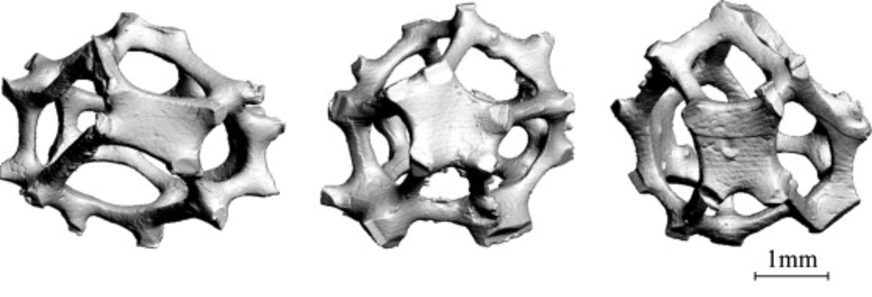
\includegraphics[width=\textwidth]{jang_open_close}
	\end{subfigure}
	\caption{{CT-scans of individual cells from a 10-ppi Al foam exhibiting open/closed intermediate faces} \cite{jangMicrostructureOpencellFoams2008}}\label{open-close1}
\end{figure}

\begin{figure}
	\centering
	\begin{subfigure}[b]{0.45\textwidth}
		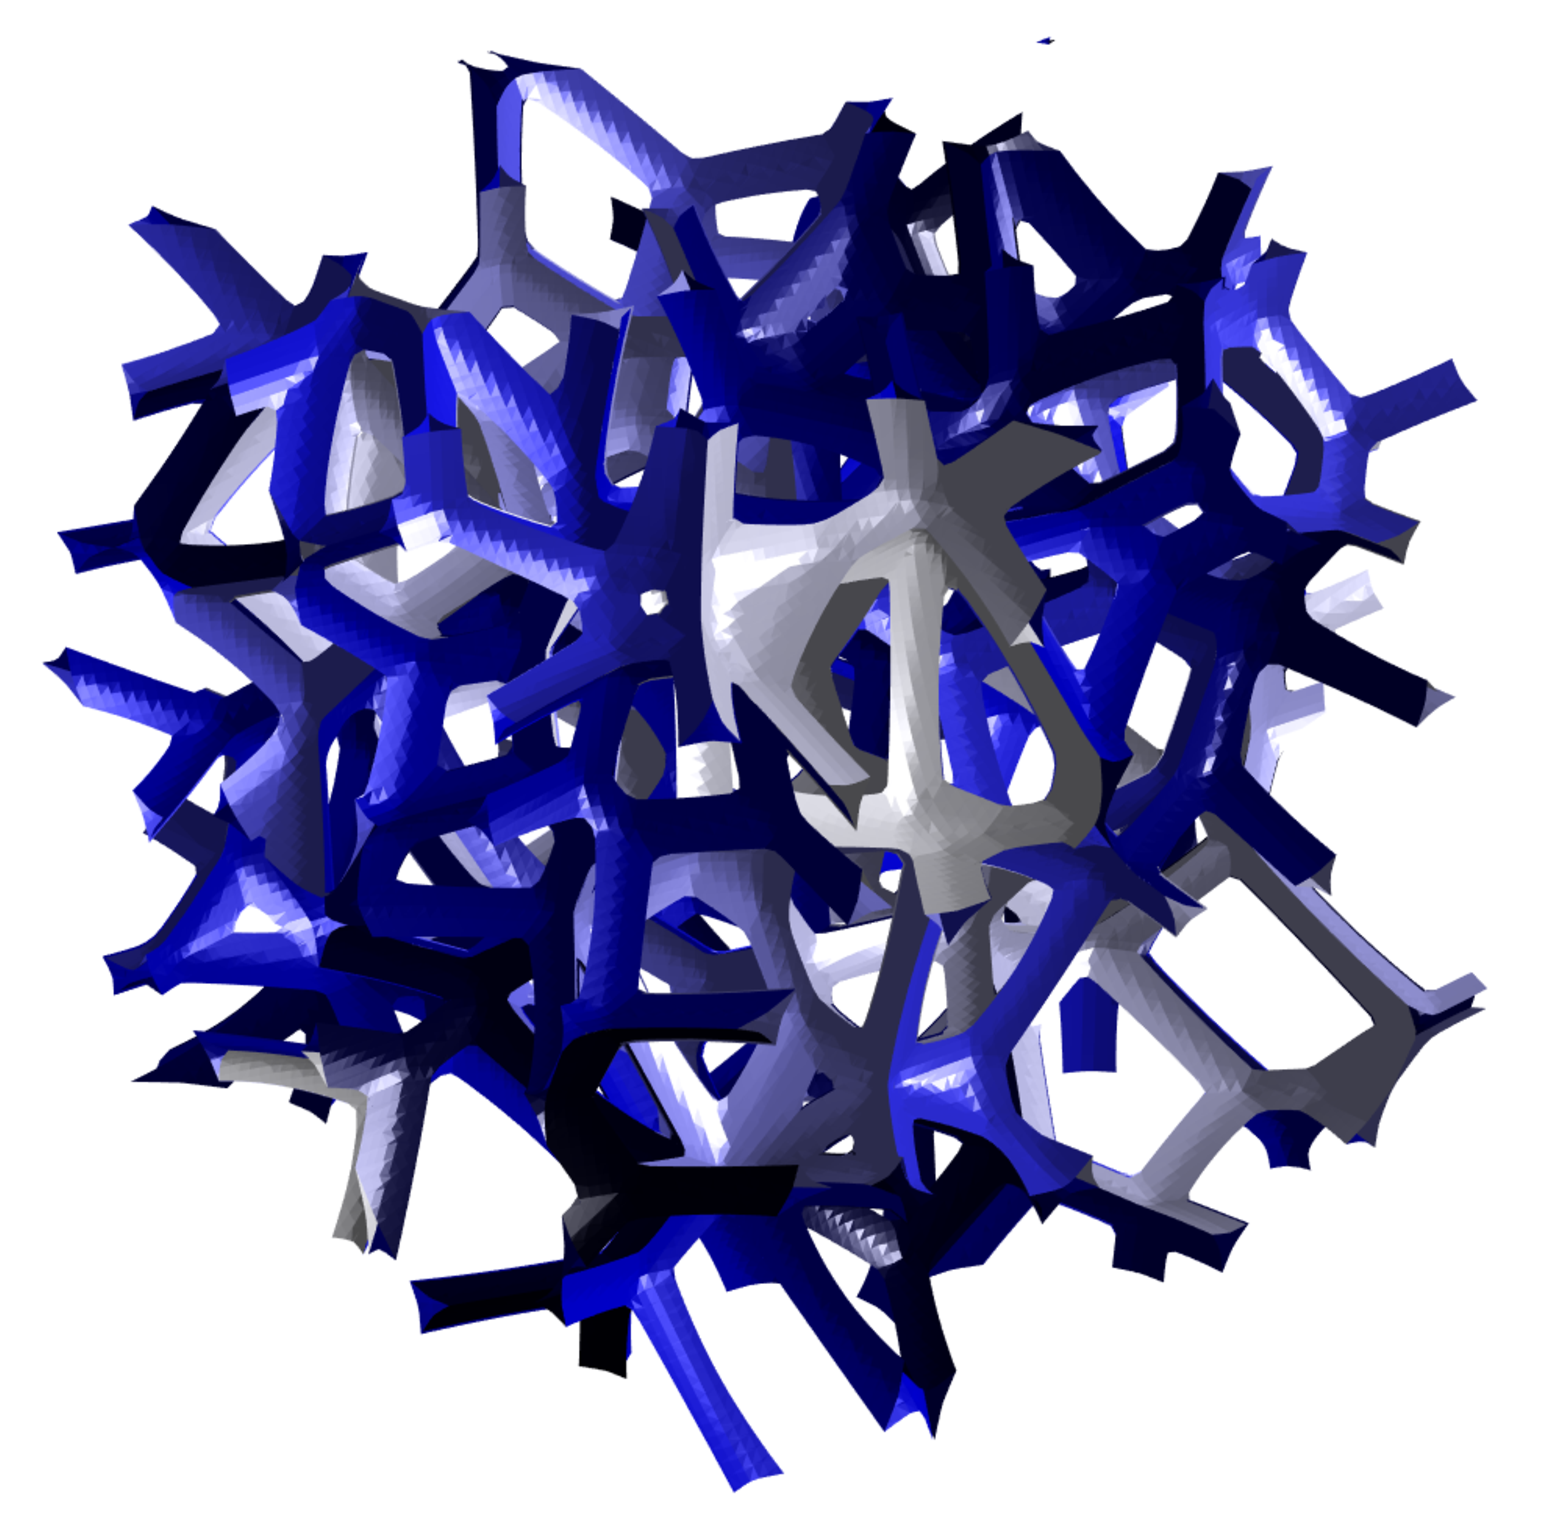
\includegraphics[width=\textwidth]{OP_CL_1}
		\caption{}
	\end{subfigure}
	\begin{subfigure}[b]{0.45\textwidth}
		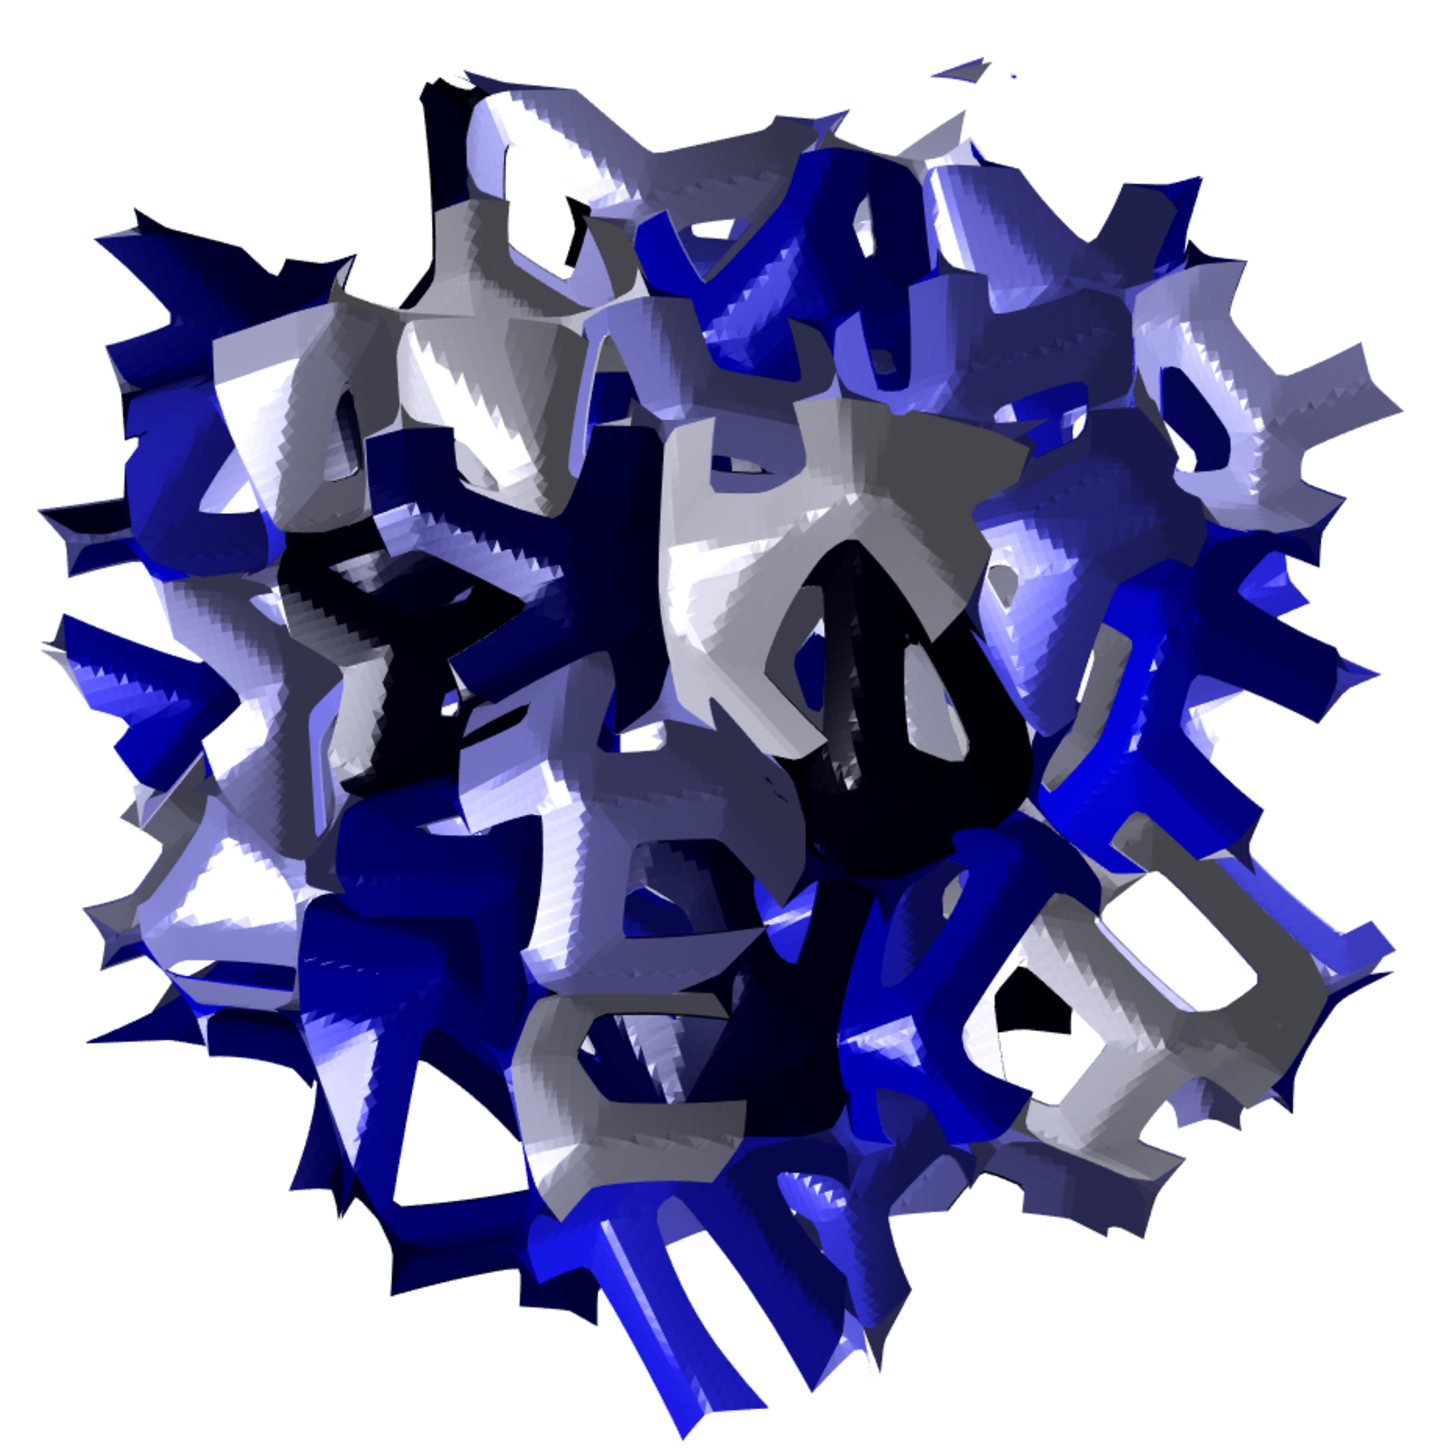
\includegraphics[width=\textwidth]{OP_CEL_2}
		\caption{}
	\end{subfigure}
	\caption{Open/Close intermediate situation using (a) $ a=0.25 $ and (b) $ a=0.5 $.}\label{open-close2}
\end{figure}


\subsection{Strut cross-sectional area distribution}\label{of-feature-strut}

\begin{figure}
	\centering
	\begin{subfigure}{\textwidth}
		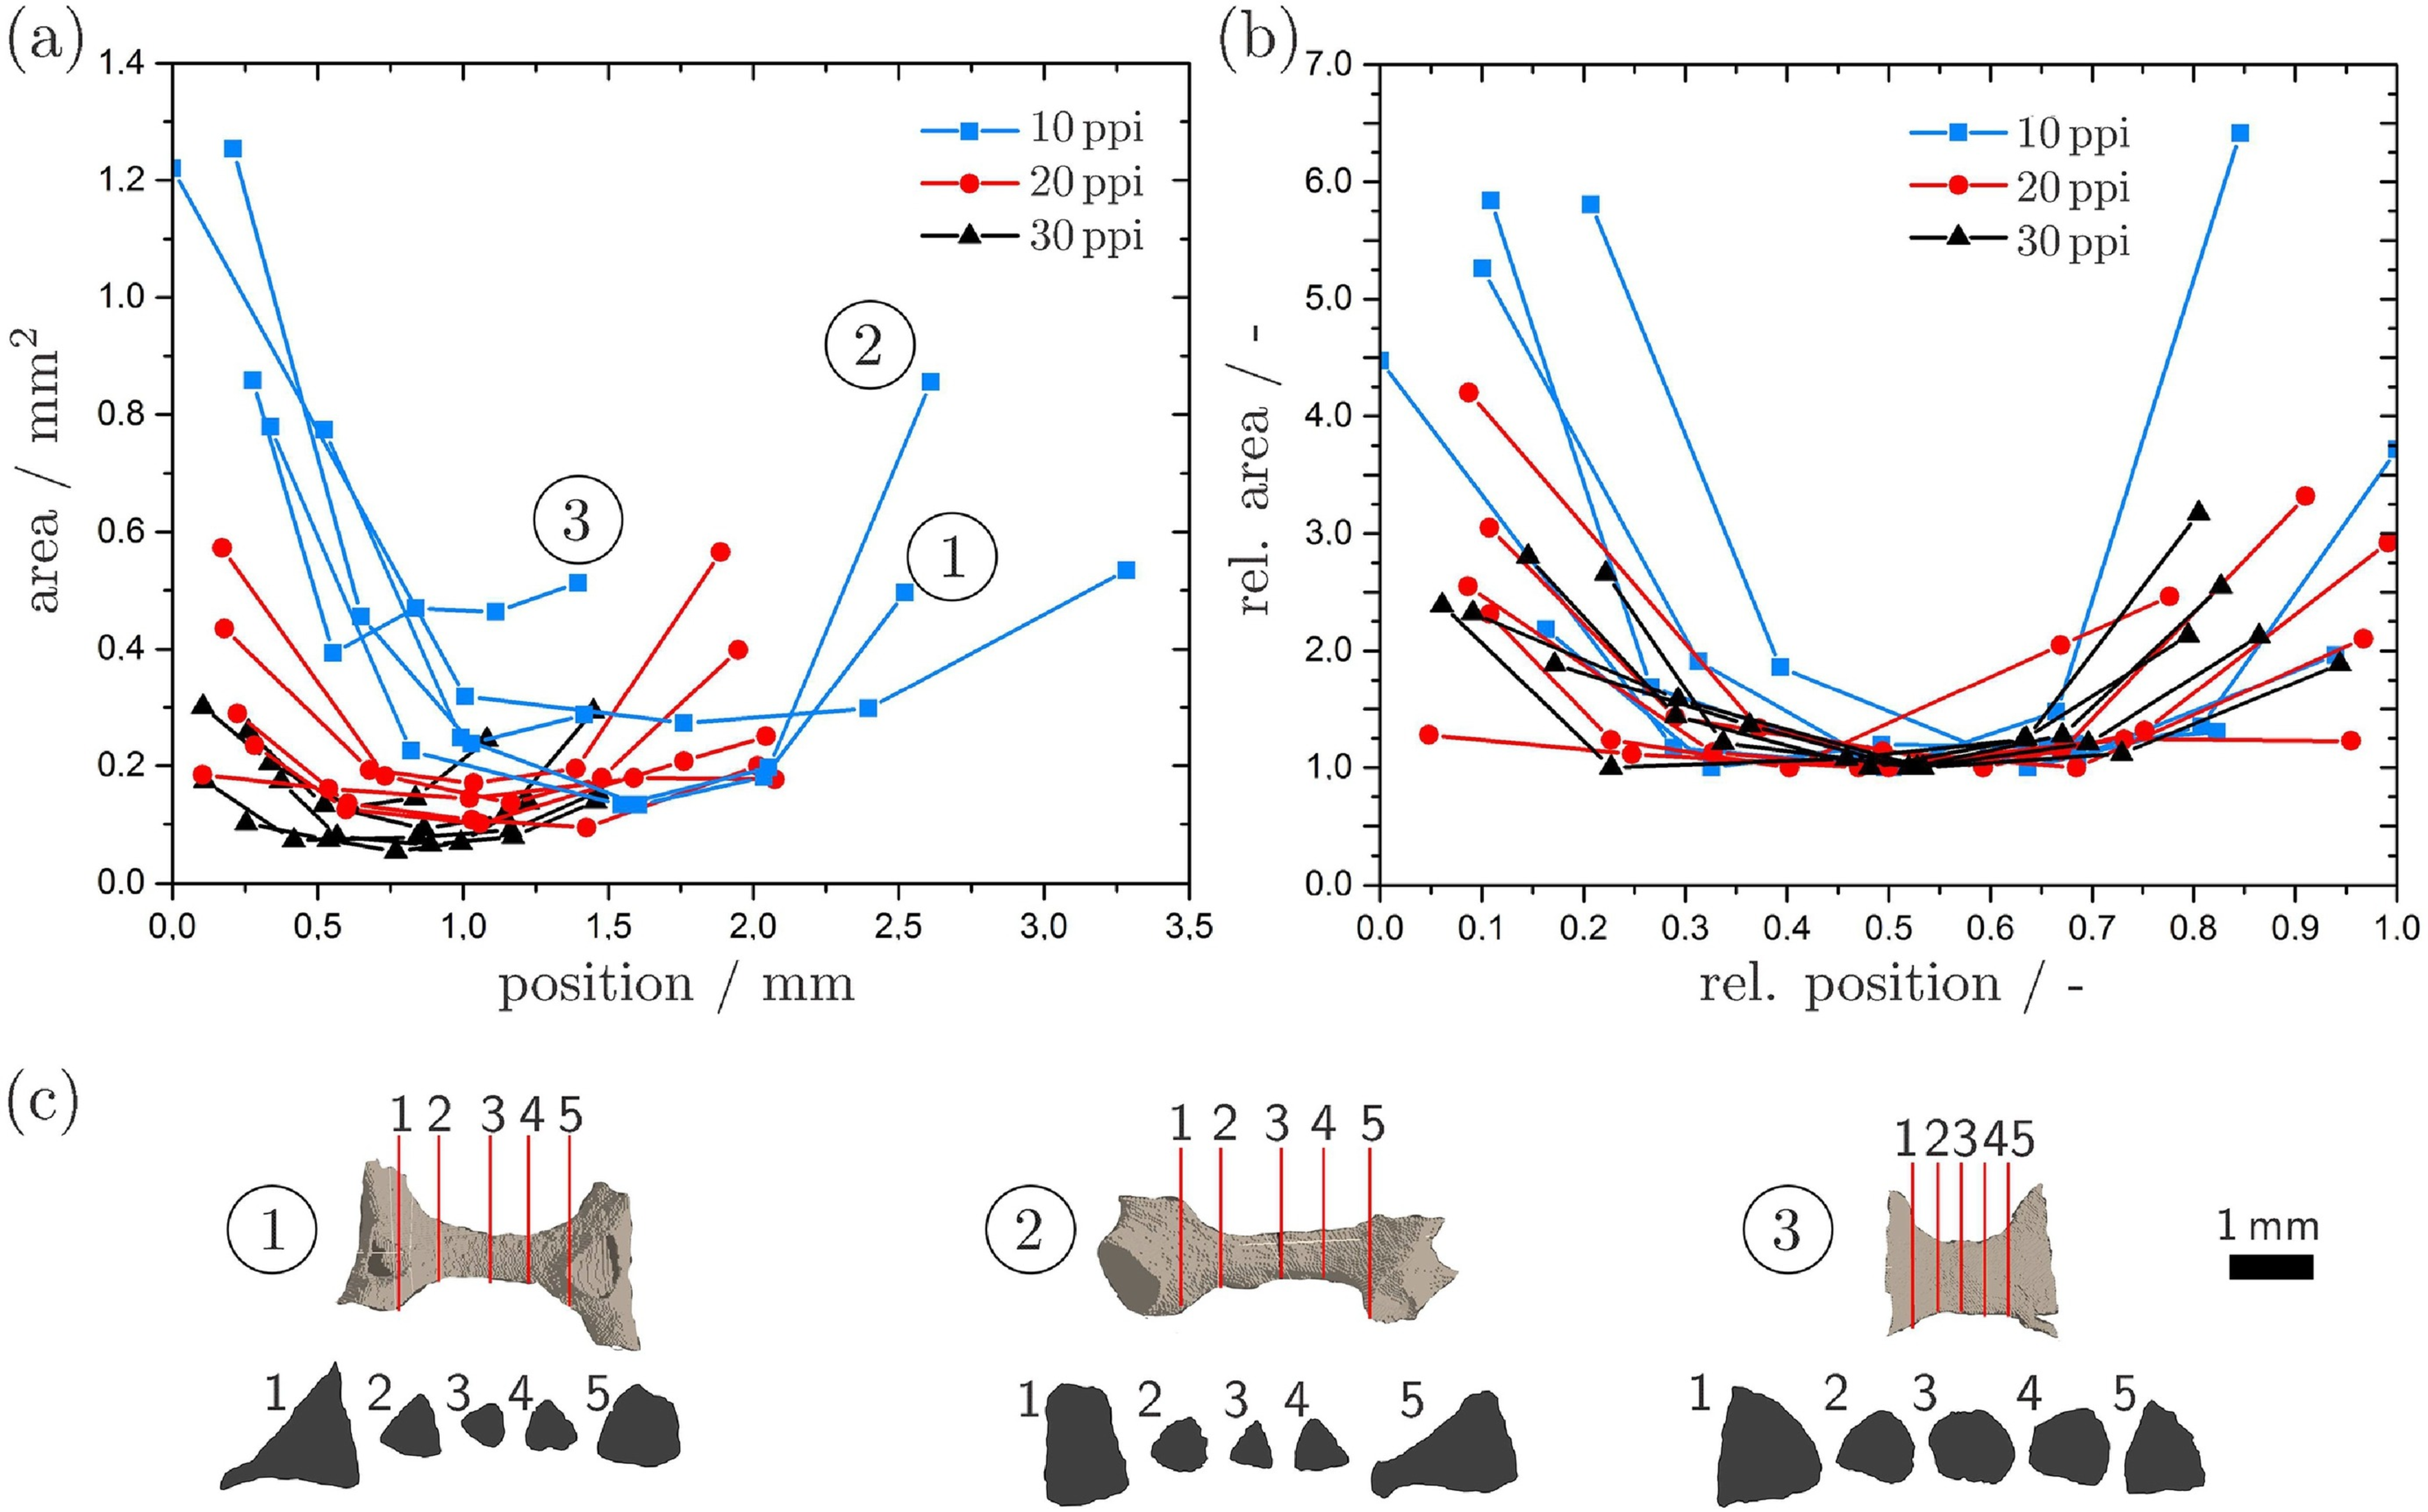
\includegraphics[width=\textwidth]{jung_ms}
	\end{subfigure}
\caption{Jung and Diebels \cite{jungMicrostructuralCharacterisationExperimental2017} analysed the strut length and distribution of the cross-sectional area along the struts for three different pore sizes of an Aluminium foam manufactured by Celltech Materials GmbH, Germany; (a) absolute values, (b) relative values normalized by the maximal length and minimal area, and (c) cross sectional profiles along three different shaped 10ppi struts}\label{strut4}
\end{figure}

Irrespective of the pore sizes, struts cross-sectional areas vary along their length. Material is concentrated in the nodes where the struts intersect while a lower material concentration is found at the mid span (Figure \ref{strut4}) \cite{jungMicrostructuralCharacterisationExperimental2017,gongCompressiveResponseOpen2005}. In \cite{jangMicrostructureOpencellFoams2008}, ligament slicing operations have been used to evaluate the ligament cross-sectional area $ A(\xi) $ normalized by the value at mid-span $ A_0 $ as a function of axial position $ \xi=x/l $, $ l $ being the ligament length:
\begin{equation}
A(\xi)=A_0(c_1 \xi^4+c_2\xi^2+1)\label{strut1},
\end{equation}
with $ c_1 $ and $ c_2 $ fitting constants. The $ \xi $ value varies from -0.5 to 0.5. Varying the values of $ c_1 $ and $ c_2 $ enables controlling the density which helps achieving various ppi models in RVEs. The studies also suggest that the longer ligaments tend to have smaller $ A_0 $ than the shorter ones \cite{jangMicrostructureOpencellFoams2008}. Fitting of the data obtained by comparing $ A_0 $ against ligament length gives a function of the form:
\begin{equation}
A_0(\eta)=\bar{A}_0(d_1+d_2\eta^{-\beta}),\,\text{ with } \eta=l/\bar{l}\label{strut2},
\end{equation}
where $ \bar{A}_0 $ and $ \bar{l} $ denote normalized mean values of all the measurements. For Al-6101-T6 Duocel open-cell foams made by ERG, the measurements were fitted with the values $ c_1=36 $, $ c_2=1 $, $ d_1 =0.6633 $, $ d_2=0.2648 $ and $ \beta=2.5963 $.

These parameters can be easily represented implicitly using the $ DN_k $ functions.\label{sec-concavity} The operator 
\begin{equation}
 O_{S1}(\textbf{x})=DN_4(\textbf{x})-DN_3(\textbf{x})  \label{variation1}
\end{equation}
varies according to the distance from the nearest node and thus, along the struts, its value increases from 0 at the nodes to half the strut length at its mid-section. If we consider the domain 
\[ \omega_{ijk}=(NN_1(\textbf{x})=i)\&(NN_2(\textbf{x})=j)\&(NN_3(\textbf{x})=k), \]
this domain represents a tetrahedral part of the tessellation cell with the vertices lying at the center of the cell generated by inclusion $ i $, the center of the face shared with the cell generated by the adjacent inclusion $ j $, and the two ends of the strut with plateau border due to the cell generated by inclusion $ k $.  The maximum value of $ O_{S1} $ in $ \omega_{ijk} $ is equal to half the length of the corresponding strut. We can therefore replace $ \eta $ in Eq. (\ref{strut2}) by 
\begin{equation}
  \eta=\frac{\max O_{S1}(\omega_{ijk})}{\text{mean}(\max O_{S1}(\omega))},
\end{equation} 
and one can reformulate $ \xi $ in Eq. (\ref{strut1}) as

\begin{equation}\label{strut-1-1}
\xi'=\frac{O_{S1}(\omega_{ijk})}{\max(O_{S1}(\omega_{ijk}))},
\end{equation}
with $ \xi' $ value varying from 0 at the nodes to 1 at the mid-span of the strut. Since this function is defined as a three dimensional one, a simple visualization is difficult to extract, but a limited visualization on the resulting isosurface of an inclusion is given in Figure \ref{strut6}.

Using the reformulated definitions and applying the new limits, the strut cross-section variation given by Eq. (\ref{strut1}) can be reformulated as
\begin{equation}
A(\xi')=A_0(e_1\xi'^4+e_2\xi'^3+e_3\xi'^2+e_4\xi'+e_5)\label{strut},
\end{equation}
with $ e_m $, $ m=1,2,\,...,\,5 $, as the reformulated coefficients of the function with changed limits. We introduce a global operator
\begin{equation}
O_S(\textbf{x}) = \sqrt{\frac{A(\xi')}{A_0}}\label{strut-operator}
\end{equation}
and combine it with Eq. (\ref{OP-2}) to control the variation of the strut cross-section in the generated morphology as:
\begin{equation}
O_P(\textbf{x})-t.O_S(\textbf{x})=0.\label{strut7}
\end{equation}

Figure \ref{strut5} shows the effect of introducing the parameters on the foam morphology and the corresponding variations in the weight density of the RVE. This enables controlling the ppi ratio with the commercially available foams, while maintaining the unit dimensions of the generated RVE necessary to perform a numerical analysis.

\begin{figure}
	\centering
	\begin{subfigure}[b]{0.45\textwidth}
		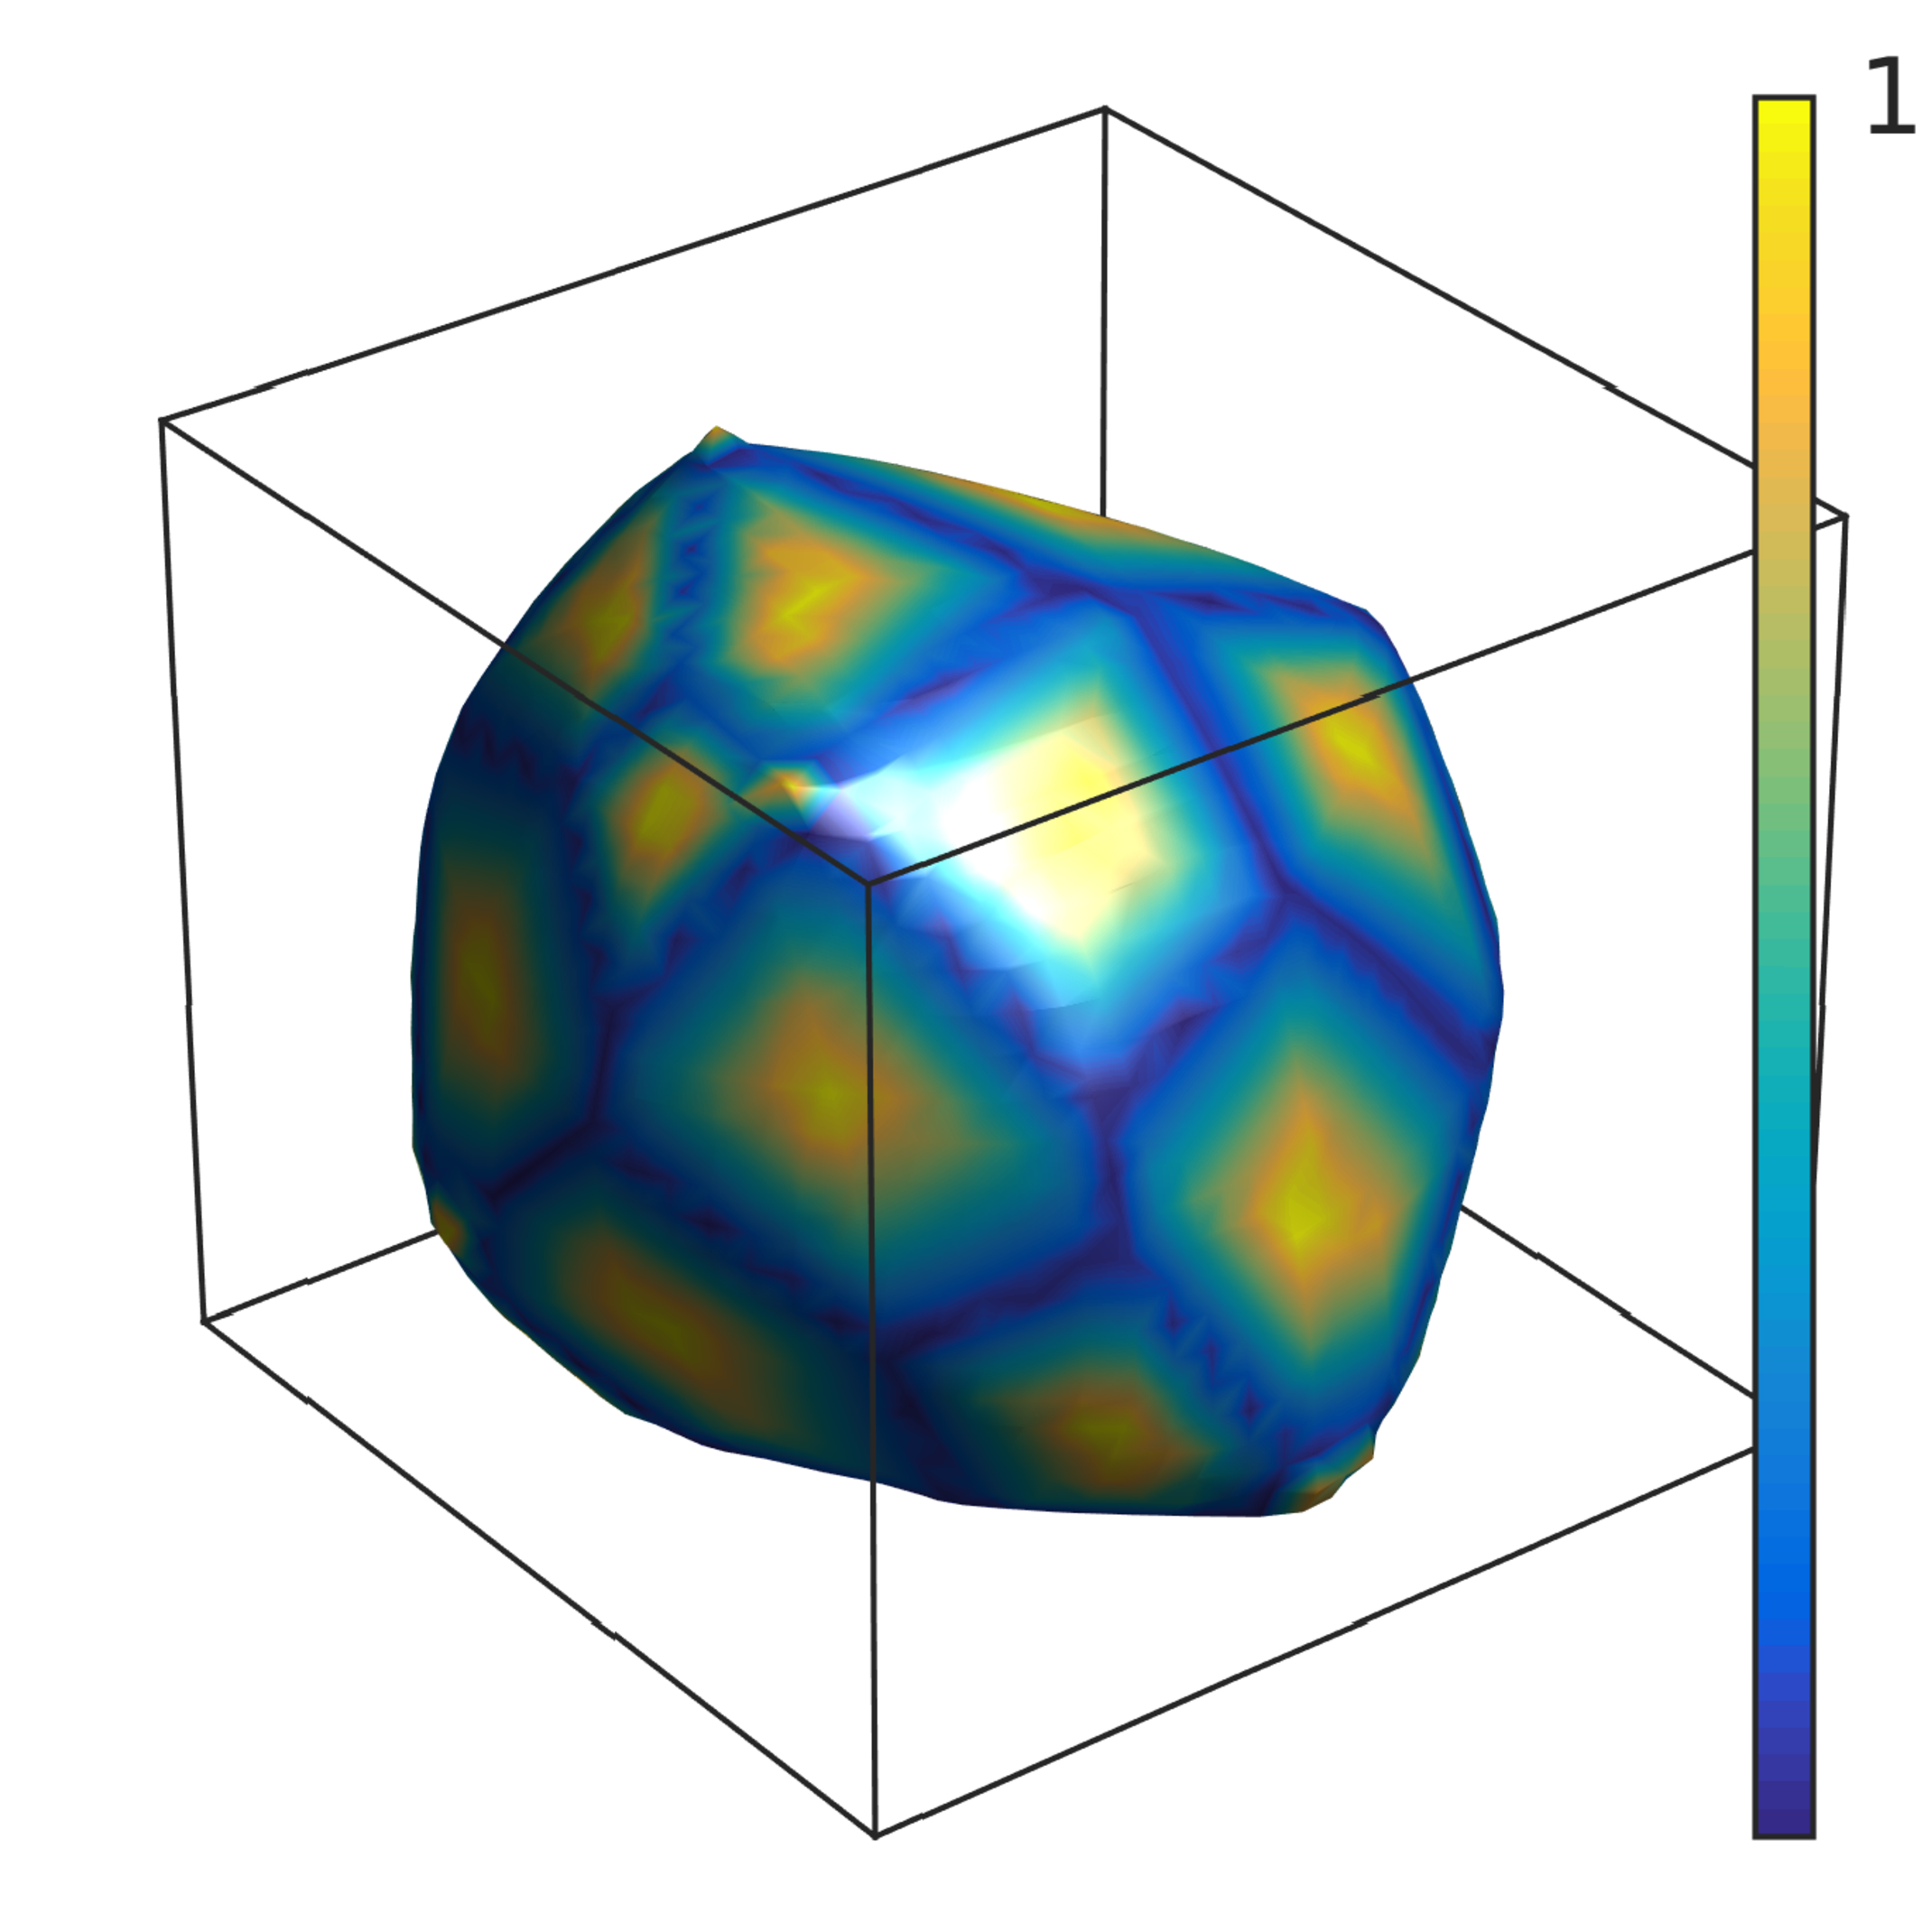
\includegraphics[width=\textwidth]{STRUT_3}
		\caption{}
	\end{subfigure}
	\begin{subfigure}[b]{0.45\textwidth}
		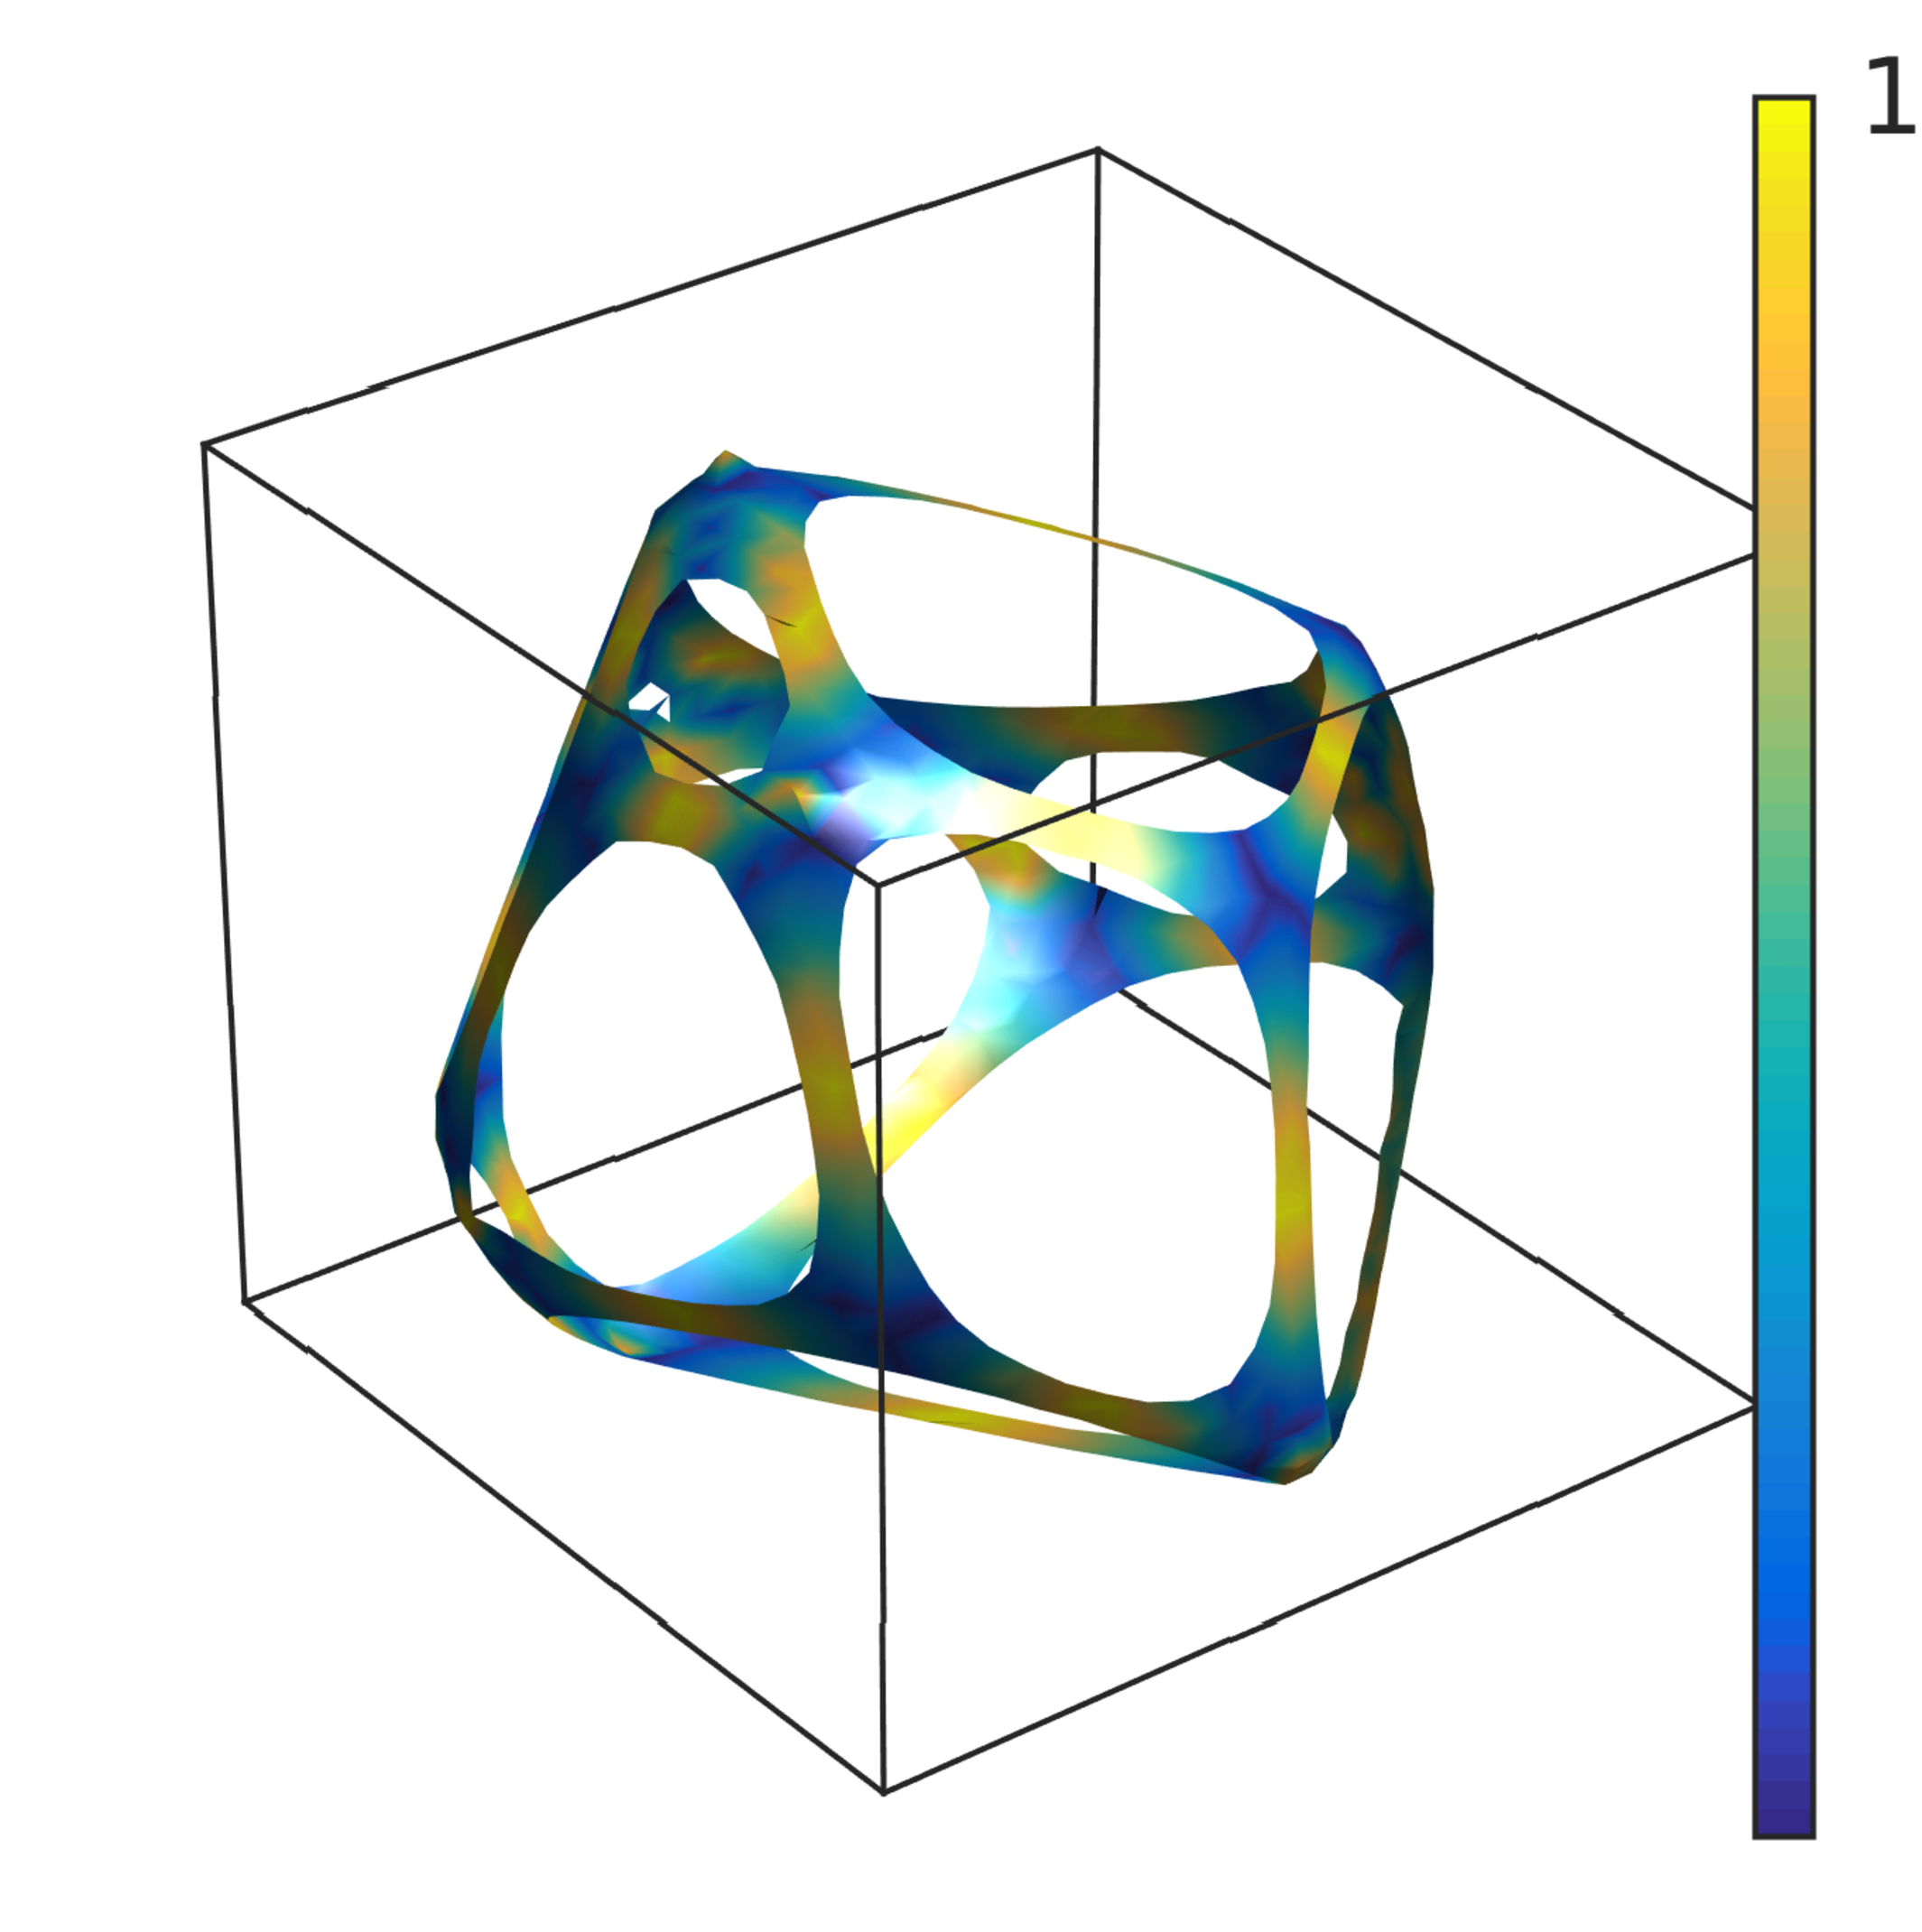
\includegraphics[width=\textwidth]{STRUT_4}
		\caption{}
	\end{subfigure}

	\caption{The variation of $ \xi' $ on the isosurface extracted using Eq. (\ref{strut-1-1}). The variation of $ \xi' $ from 0 to 1 along the strut surface can be observed. A sliced surface of the same inclusion is given for comparison. }\label{strut6}
\end{figure}

\begin{figure}
	\centering
	\begin{subfigure}[b]{0.49\textwidth}
		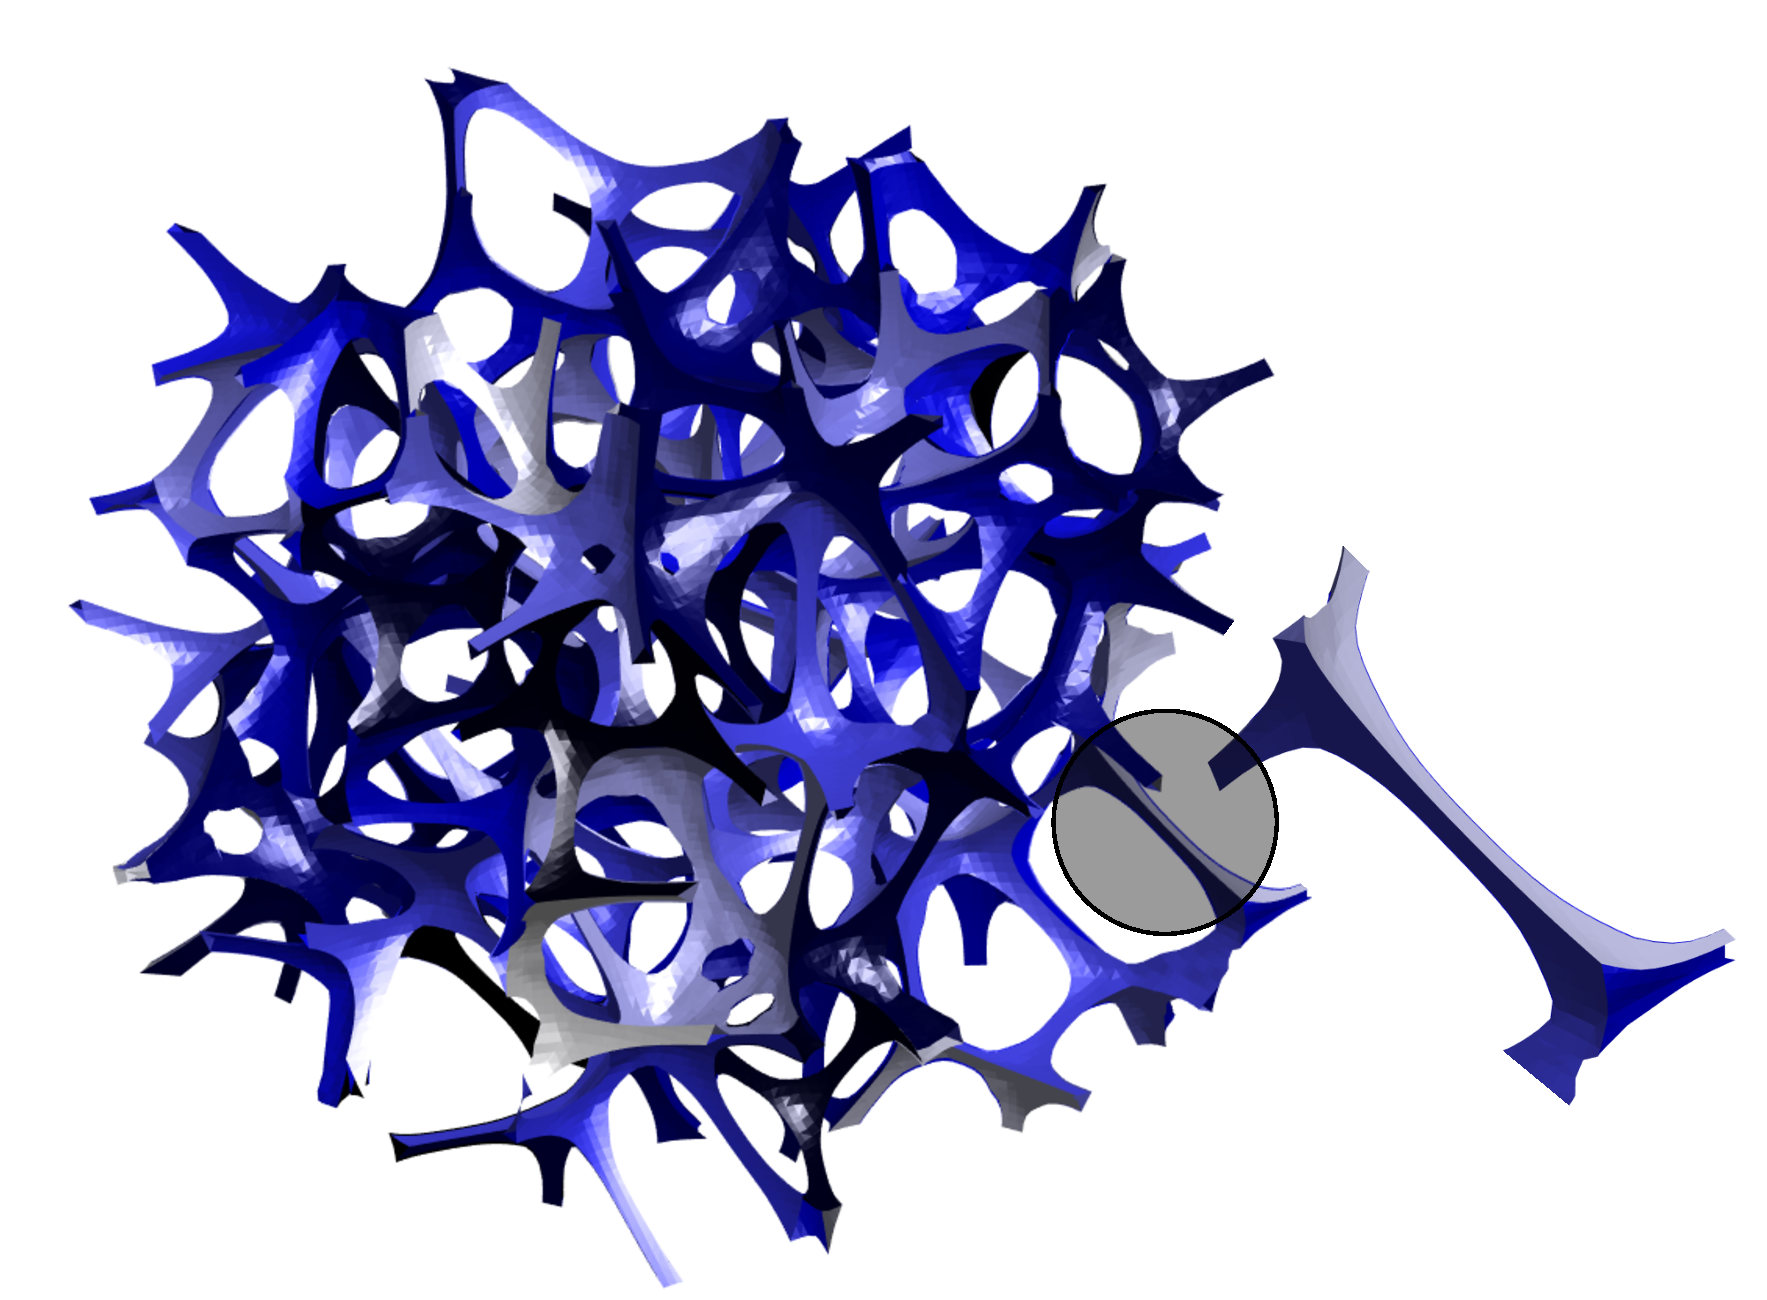
\includegraphics[width=\textwidth]{STRUT_1}
		\caption{}
	\end{subfigure}
	\begin{subfigure}[b]{0.49\textwidth}
		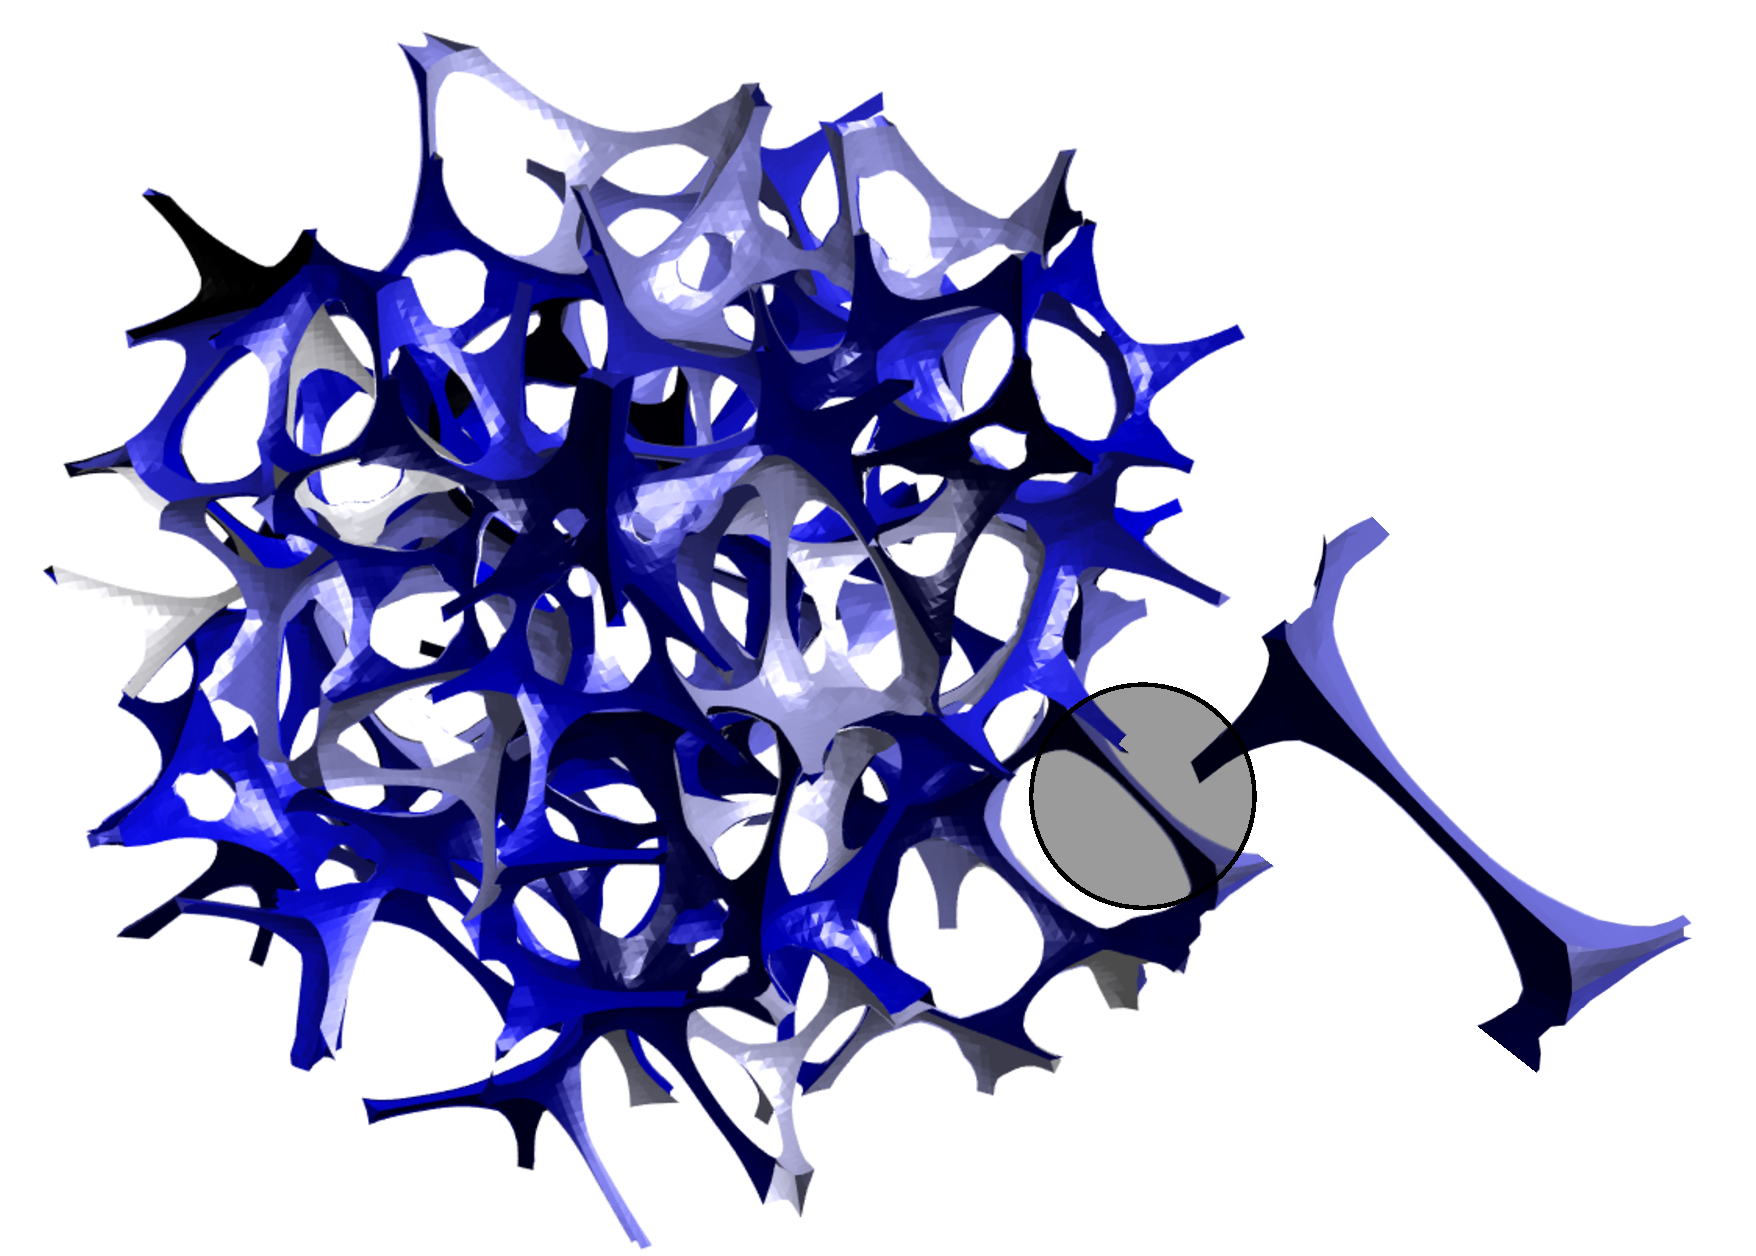
\includegraphics[width=\textwidth]{STRUT_2}
		\caption{}
	\end{subfigure}

	\caption{Effect of Eq. (\ref{strut1}) on the strut cross-section with (a) $ c_1=20 $ and $ c_2 = 1 $, and (b) $c_1=50  $ and $ c_2=1 $.}\label{strut5}
\end{figure}

\subsection{Strut concavity}\label{of-feature-strutcon}

\begin{figure}
	\centering
	\begin{subfigure}[b]{0.45\textwidth}
		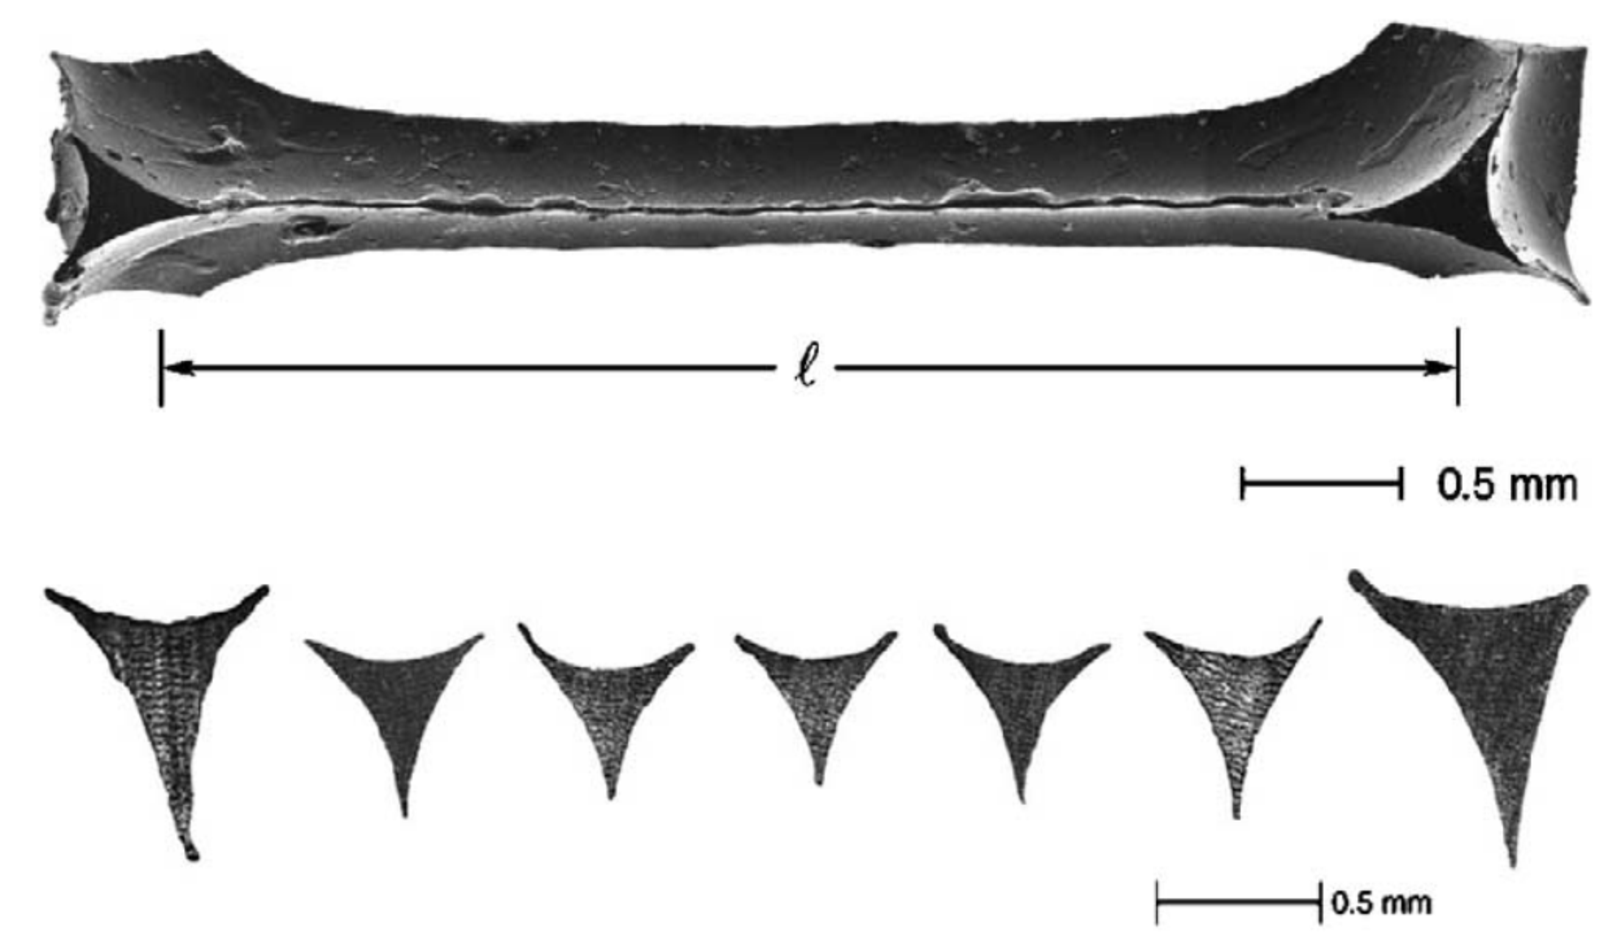
\includegraphics[width=\textwidth]{jang_foam_PU}
		\caption{}
	\end{subfigure}
	\begin{subfigure}[b]{0.45\textwidth}
	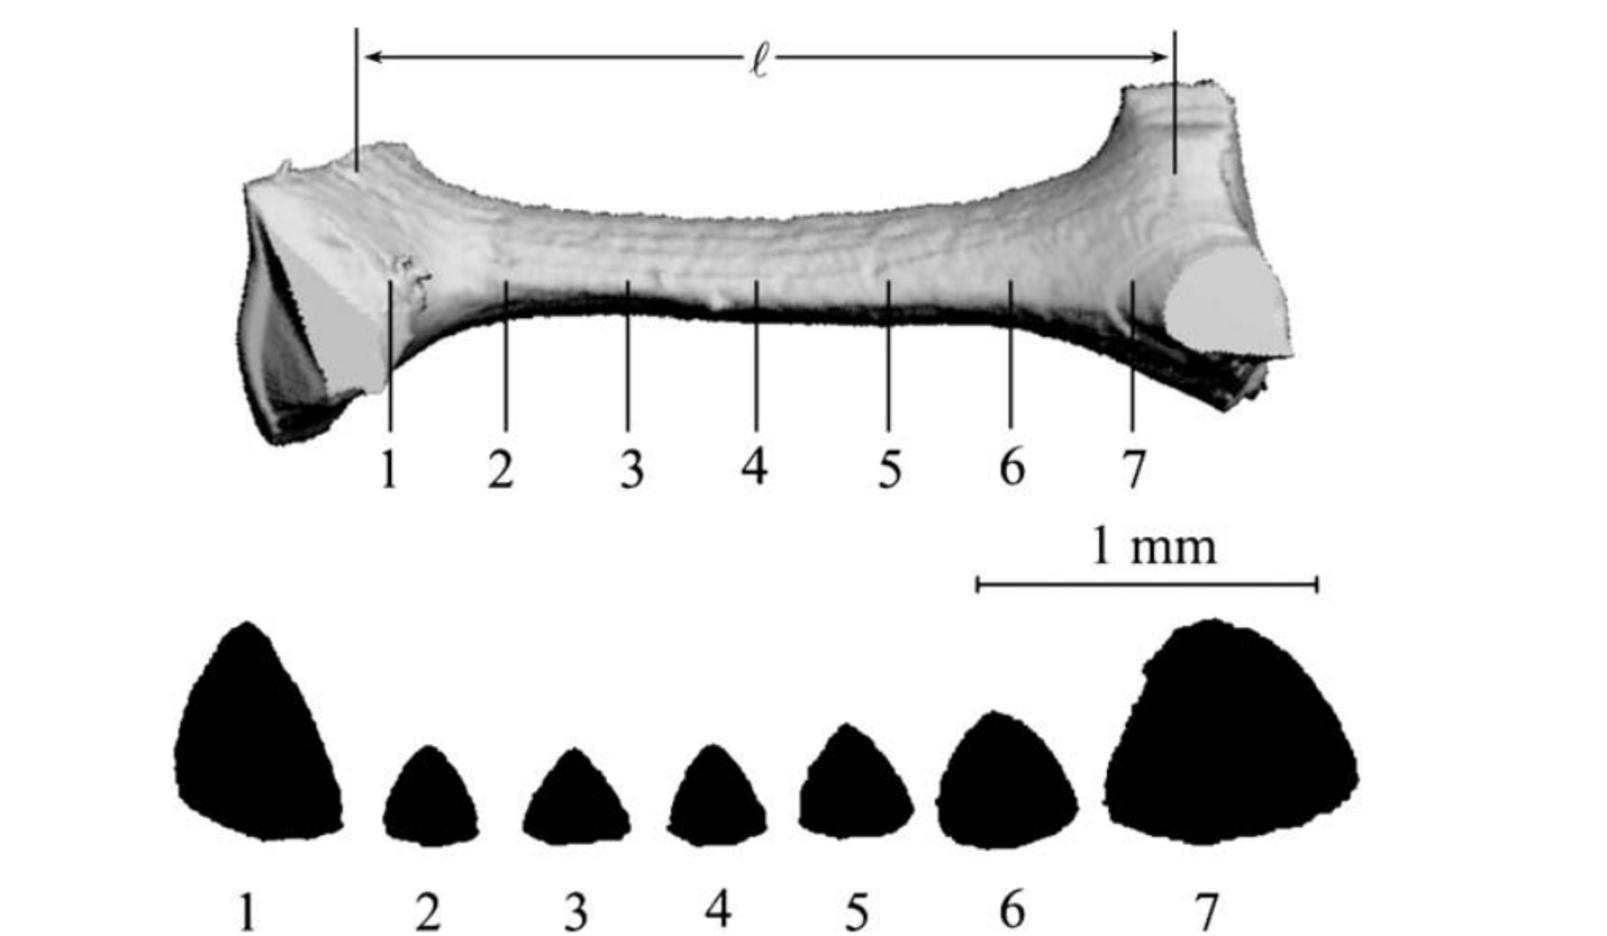
\includegraphics[width=\textwidth]{jang_foam_alu}
	\caption{}
\end{subfigure}
	\caption{(a) A typical polyurethane open cell foam strut and the cross-sections along the length of the strut\cite{gongCompressiveResponseOpencell2005}; (b) A typical aluminum open cell foam strut and the cross-sections along the length of the strut\cite{jangCrushingAluminumOpencell2009}.}\label{strut3}
\end{figure}

Polyurethane (PU) ligaments usually have a 3-cusp hy\-po\-cy\-cloid cross-section varying along the length of the strut, while most of the metallic foams have a triangular cross-section that tends towards circular with increasing ppi value (Figure \ref{strut3}). To obtain such morphological variations, we can subtract a non-constant $ C^2 $ continuous function that is free from curvature jumps and unwanted sharp edges from the function defined in Eq. (\ref{strut7}). Such a function can be defined based on the maintained distance fields according to:
\begin{equation}
O_K(\textbf{x})=\min\left(0,\frac{{\left(\left(\frac{DN_3(\textbf{x})-DN_2(\textbf{x})}{2}\right)^2-\left(t.O_S(\textbf{x})\right)^2\right)}}{{2t.O_S(\textbf{x})}}\right)\label{plateau},
\end{equation}
which can now be combined with Eq. (\ref{strut7}) to control the plateau border concavity by using:
\begin{equation}
O_P(\textbf{x})-t.O_S(\textbf{x})-k_c.O_K(\textbf{x})=0,\label{concavity-eq}
\end{equation}
with $ 0<k_c<1 $ as the concavity controlling parameter. The effect of concavity as well as of strut cross-section variation is illustrated in Figure \ref{concavity}. {Operator (\ref{concavity-eq}) is acceptable for simple cross-sectional geometries like triangular, concave triangular or circular shapes. Slight variations with $ k_c<0 $ can also be studied to analyze RVEs with struts having convex triangular cross-sections.}

\begin{figure}
	\centering
	\begin{subfigure}[b]{0.45\textwidth}
		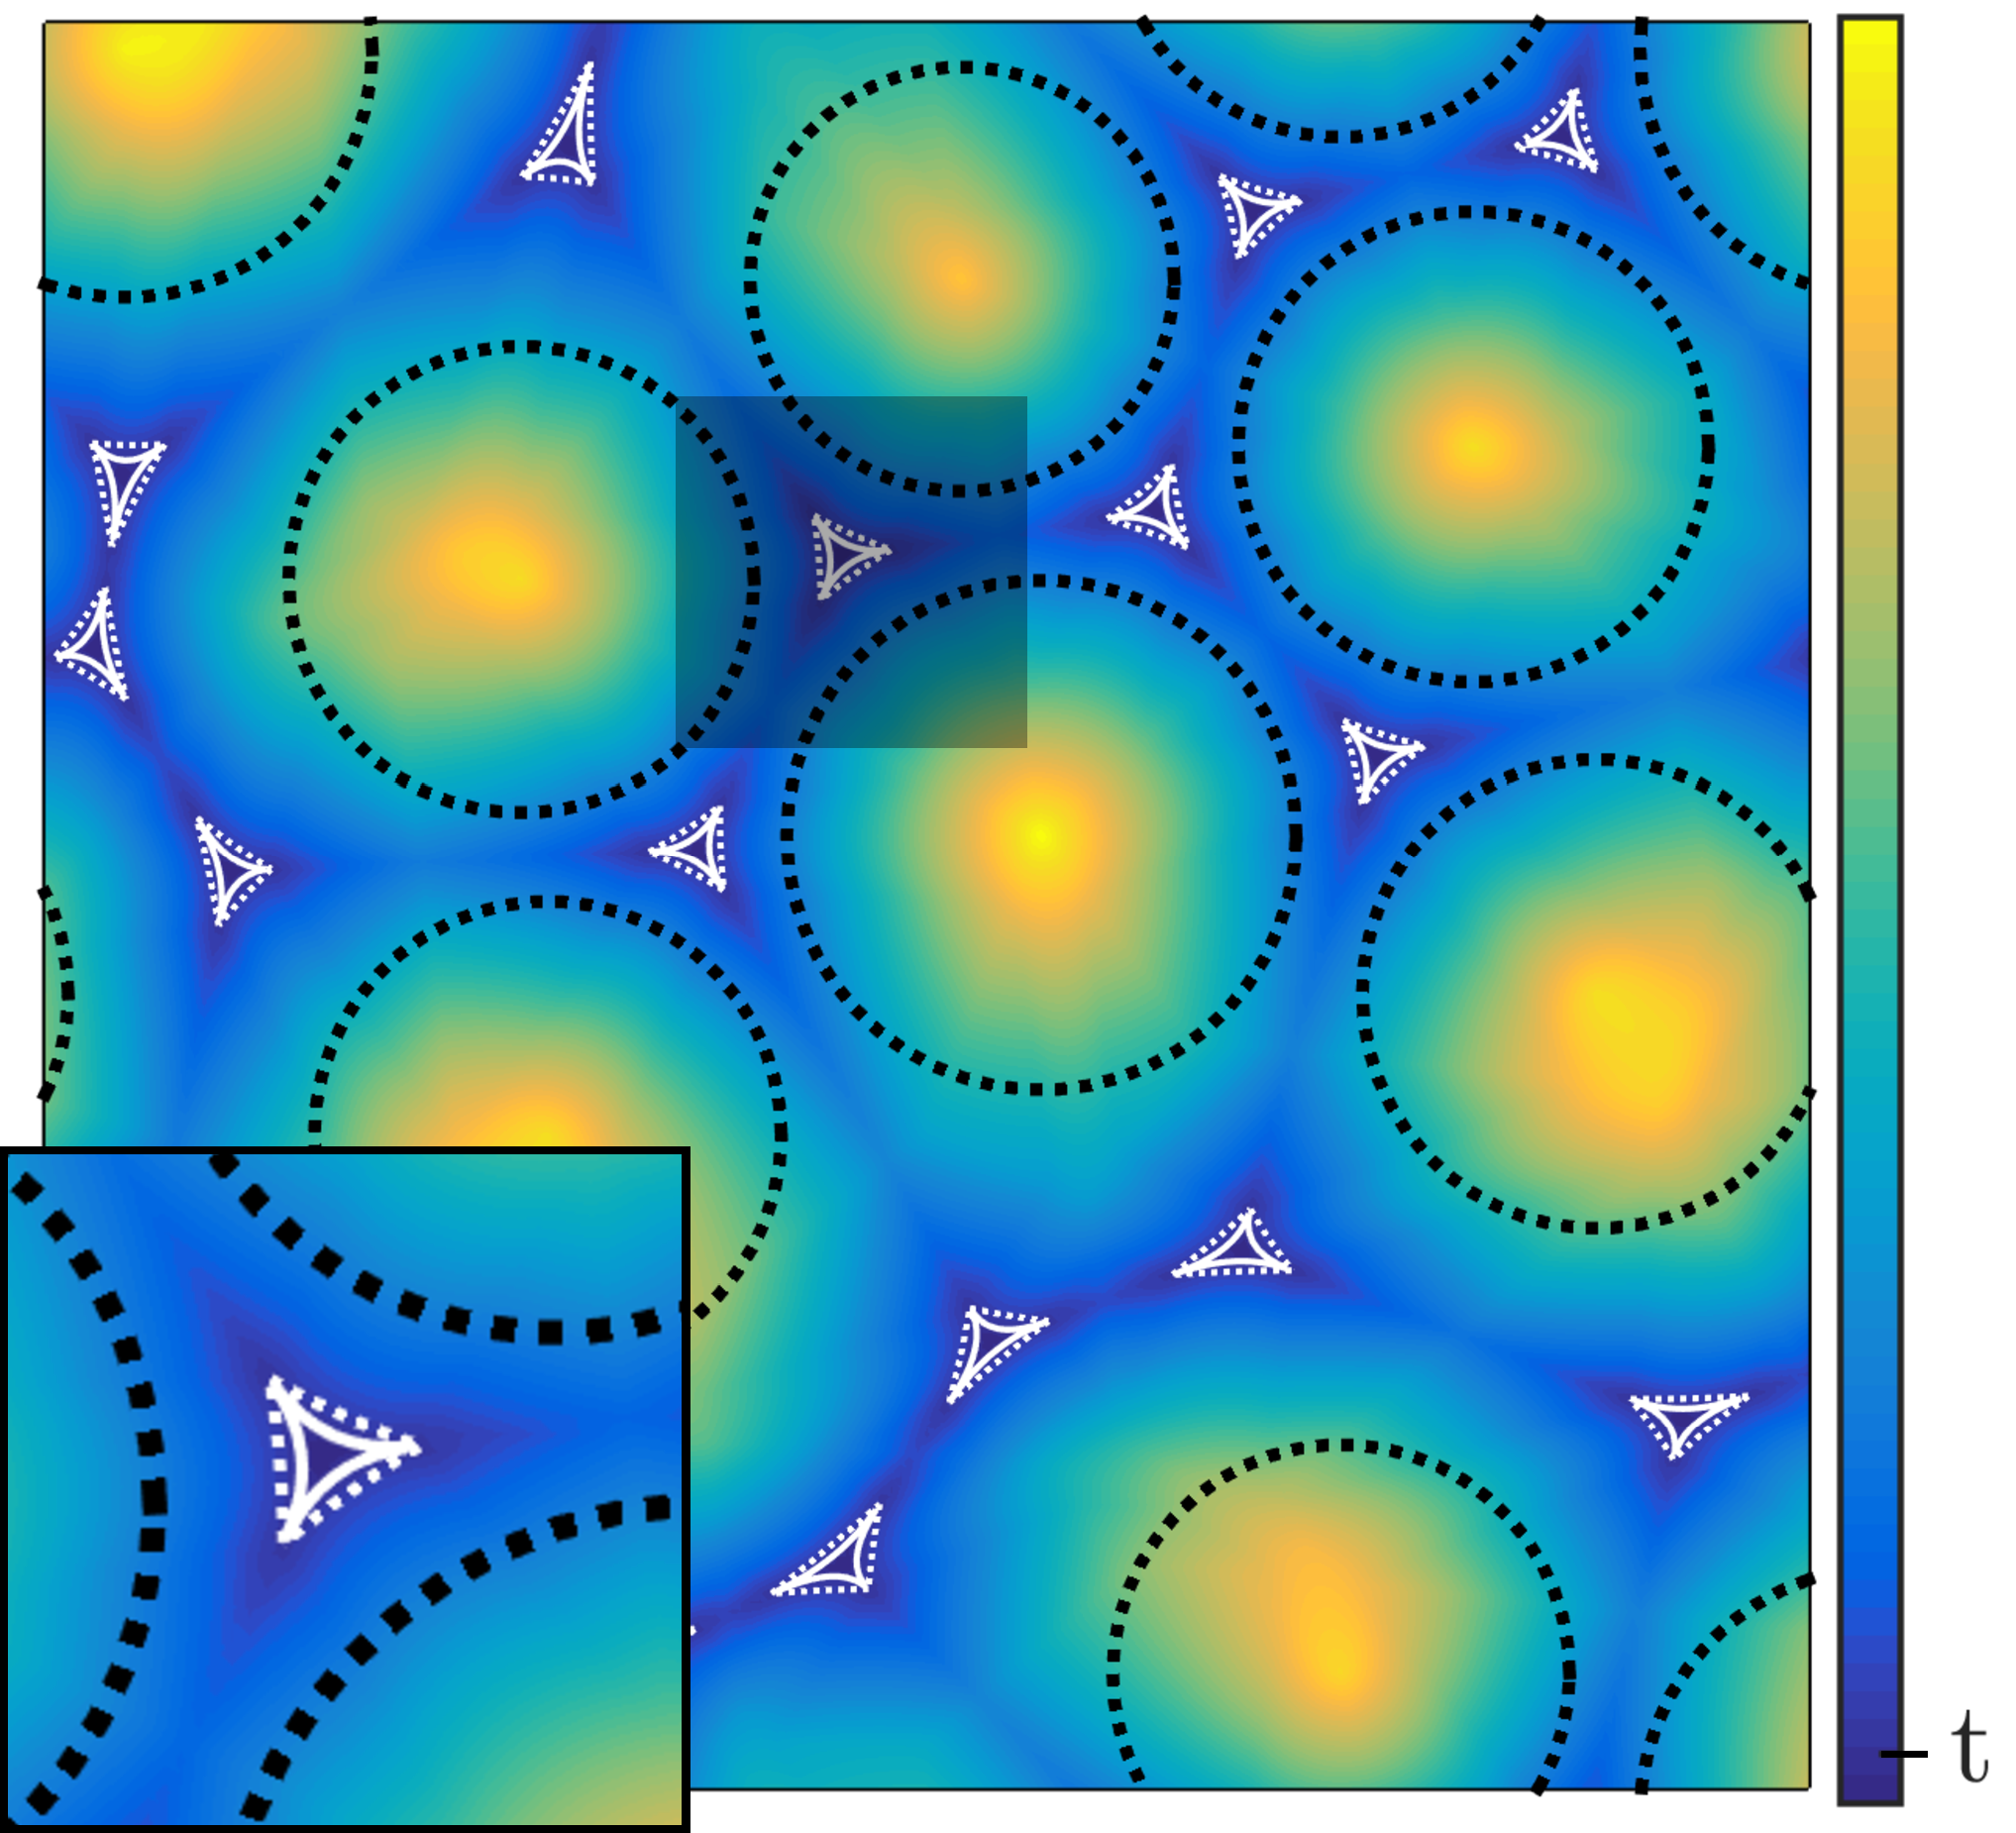
\includegraphics[width=\textwidth]{OP_Plateau}
		\caption{}
	\end{subfigure}
	\begin{subfigure}[b]{0.45\textwidth}
		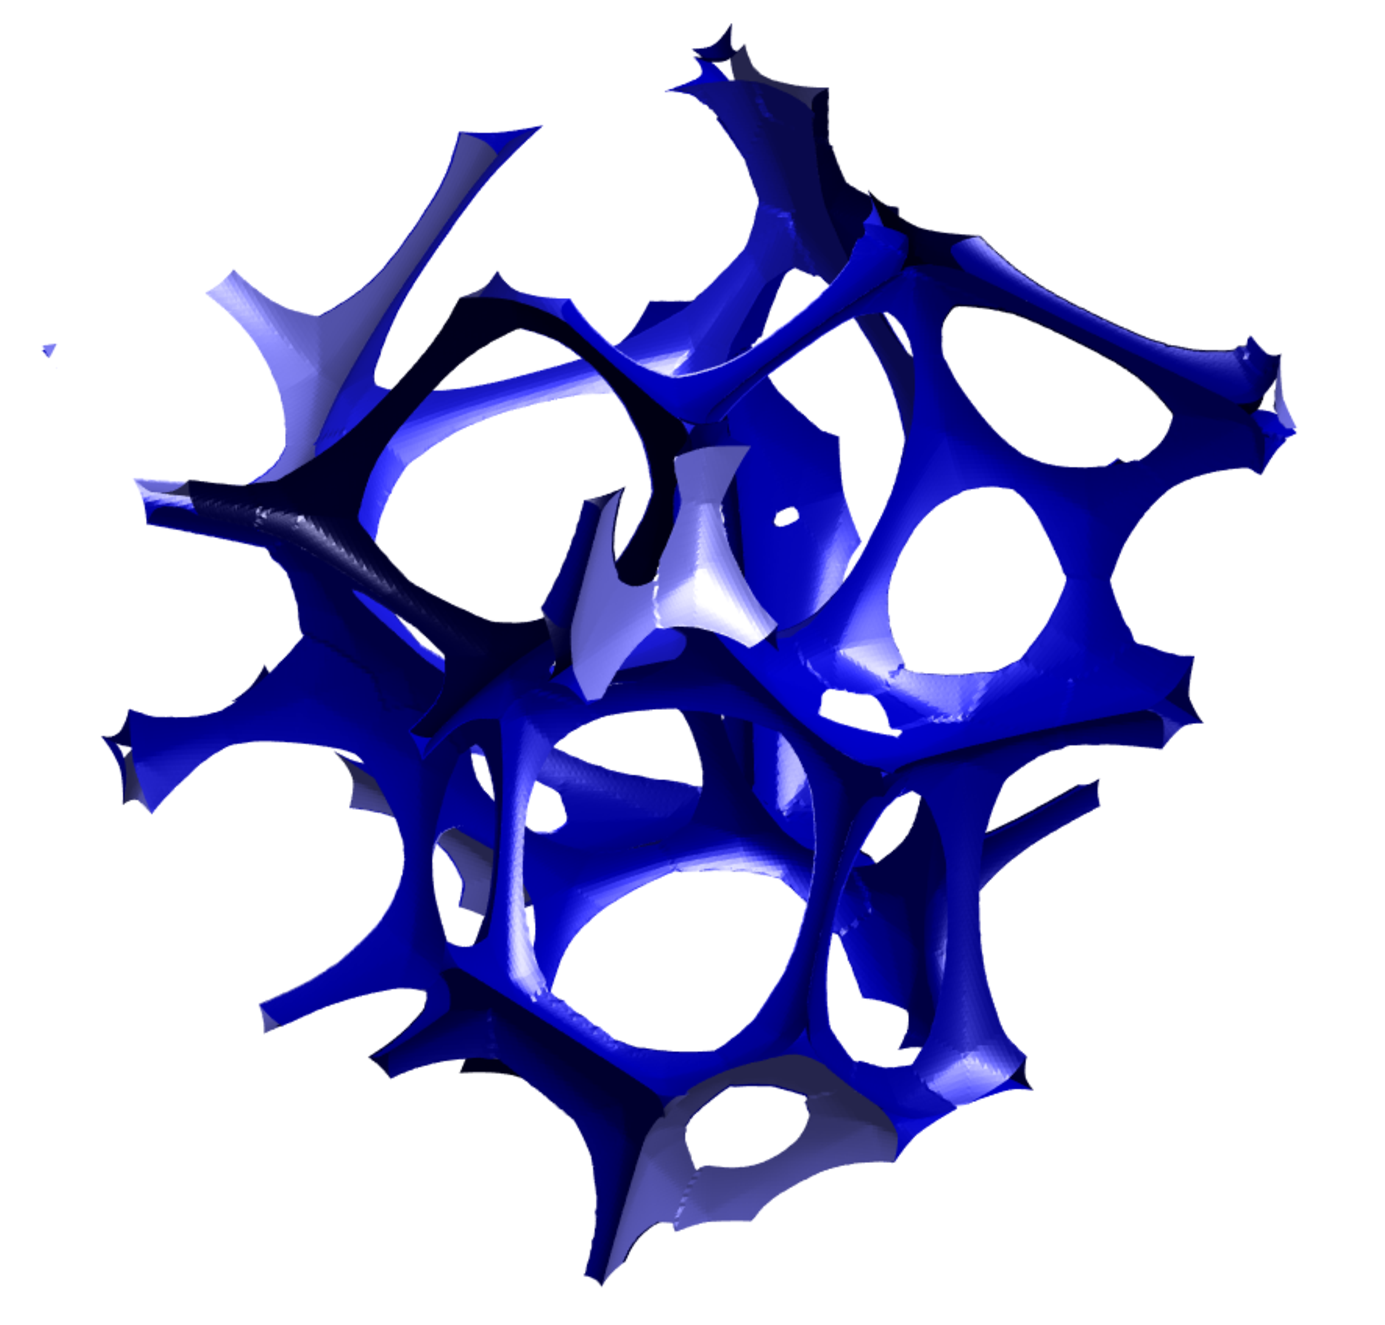
\includegraphics[width=\textwidth]{OP_Plateau_3D}
		\caption{}
	\end{subfigure}
	\caption{Plateau border concavity control; (a) white lines denote concavity with $ k_c=1 $ while dashed lines denote simple plateau border, and (b) 3D detail with $ k_c=0.5 $, $ c_1 = 20 $ and $ c_2=1 $ , $ d_1=0.6633 $, $ d_2=0.2648 $ and $ \beta=2.5963 $, the data being obtained from statistical analysis of the entire foam sample \cite{jangMicrostructureOpencellFoams2008}. }\label{concavity}
\end{figure}
\subsection{Anisotropy}\label{of-feature-anisotropy}
The metallic foams manufactured by investment casting over a PU base display anisotropic characteristics in the rise direction \cite{jangMicrostructureOpencellFoams2008}. Although naturally accounted for when using the inclusions packing obtained from the CT-scan images, {this anisotropy can be implemented in the RVE obatined using DN-RSA in the initial packing generation by the use of anisotropic packings instead of spherical packing. An anisotropy parameter can also be introduced in the distance functions, which is simply the percentage of the original length, once the packing is generated, in a particular direction so that the RVE generated using the function $ O_P $ leads to the extraction of an anisotropic RVE. Anisotropy in foam can also exist in the form of partially reticulated, or intermediary states, between open and closed walls in some of the pores \cite{jangCompressiveStrengthOpencell2010}, the implementation of which can be found in \cite{sononAdvancedApproachGeneration2015}}.

\section{Sharp edge extraction by means of local level set functions}\label{of-sharp}
\sectionmark{Sharp edge extraction}
The steep discontinuity of $ DN_k $ derivatives on $ \Phi_\Theta $ cannot be handled by the use of level set functions evaluated on discrete grids of points, and thus the sharp edges of the Plateau borders geometry cannot be extracted with simple contouring algorithms (Figure \ref{sharp1}a). This problem is illustrated in Figure \ref{sharp1}b where jagged edges are obtained when a classical contouring is applied. This prevents the discretization by means of a proper finite element mesh. To overcome this issue, the global geometry can be split into an assembly of smooth surfaces extracted from separate ``Local" level set functions as proposed in \cite{sononAdvancedApproachGeneration2015}. 
%The three faces of each Plateau border are determined by the surfaces extracted from the three nearest inclusions at that point. 
By constructing an individual local level set for each inclusion, the problem arising due to sharp edges can be avoided (Figure \ref{sharp2}). However, in order to obtain the holes on the resulting surfaces that exist in the open foam, additional slicing operations need to be carried out. Two methods can be suggested for such an operation:
\begin{enumerate}
	\item Construction of a second ``outer'' level set function for each inclusion which is used to slice the surface obtained by the first ``inner'' level set function. By interpolating the values of the second function on the vertices of the surface obtained from the first function, the slicing operation can be carried out using a ``marching algorithm" \cite{sononAdvancedApproachGeneration2015}\label{outer}. When using this method, once the surface coming from inclusion $ i $ is extracted, it is not necessary to store both ``inner" and ``outer'' functions in memory. For large RVEs though, especially in 3D, this creates the issue of mismatch of vertices of a common sharp edge between two surfaces	due to the discrete evaluation of the extracted functions. In such cases, for classical contouring implementations, there is no guarantee that the two smooth surfaces belonging to adjacent inclusions meeting at the sharp edge will have the same discretization at their common boundary.
	\item The surface of an inclusion can be sliced by comparing it with the surface of the neighboring inclusion using Boolean intersection of surfaces. This operation, while using the same concept as in option \ref{outer}, results in the generation of surfaces with holes that form the sharp edges of the struts, perfectly aligned with the corresponding sharp edge from the surface of the neighboring inclusion.\label{inner} This approach is slightly more costly in comparison with the first method because, for each inclusion, all the neighboring ``local" functions have to be called iteratively. However, it is advantageous as the surfaces extracted for two neighboring inclusions would have common edge vertices, facilitating the post processing in the form of mesh refinement of these edges. This second approach will be used in the following sections.
\end{enumerate}


\begin{figure}
	\centering
	\begin{subfigure}[b]{0.33\textwidth}
		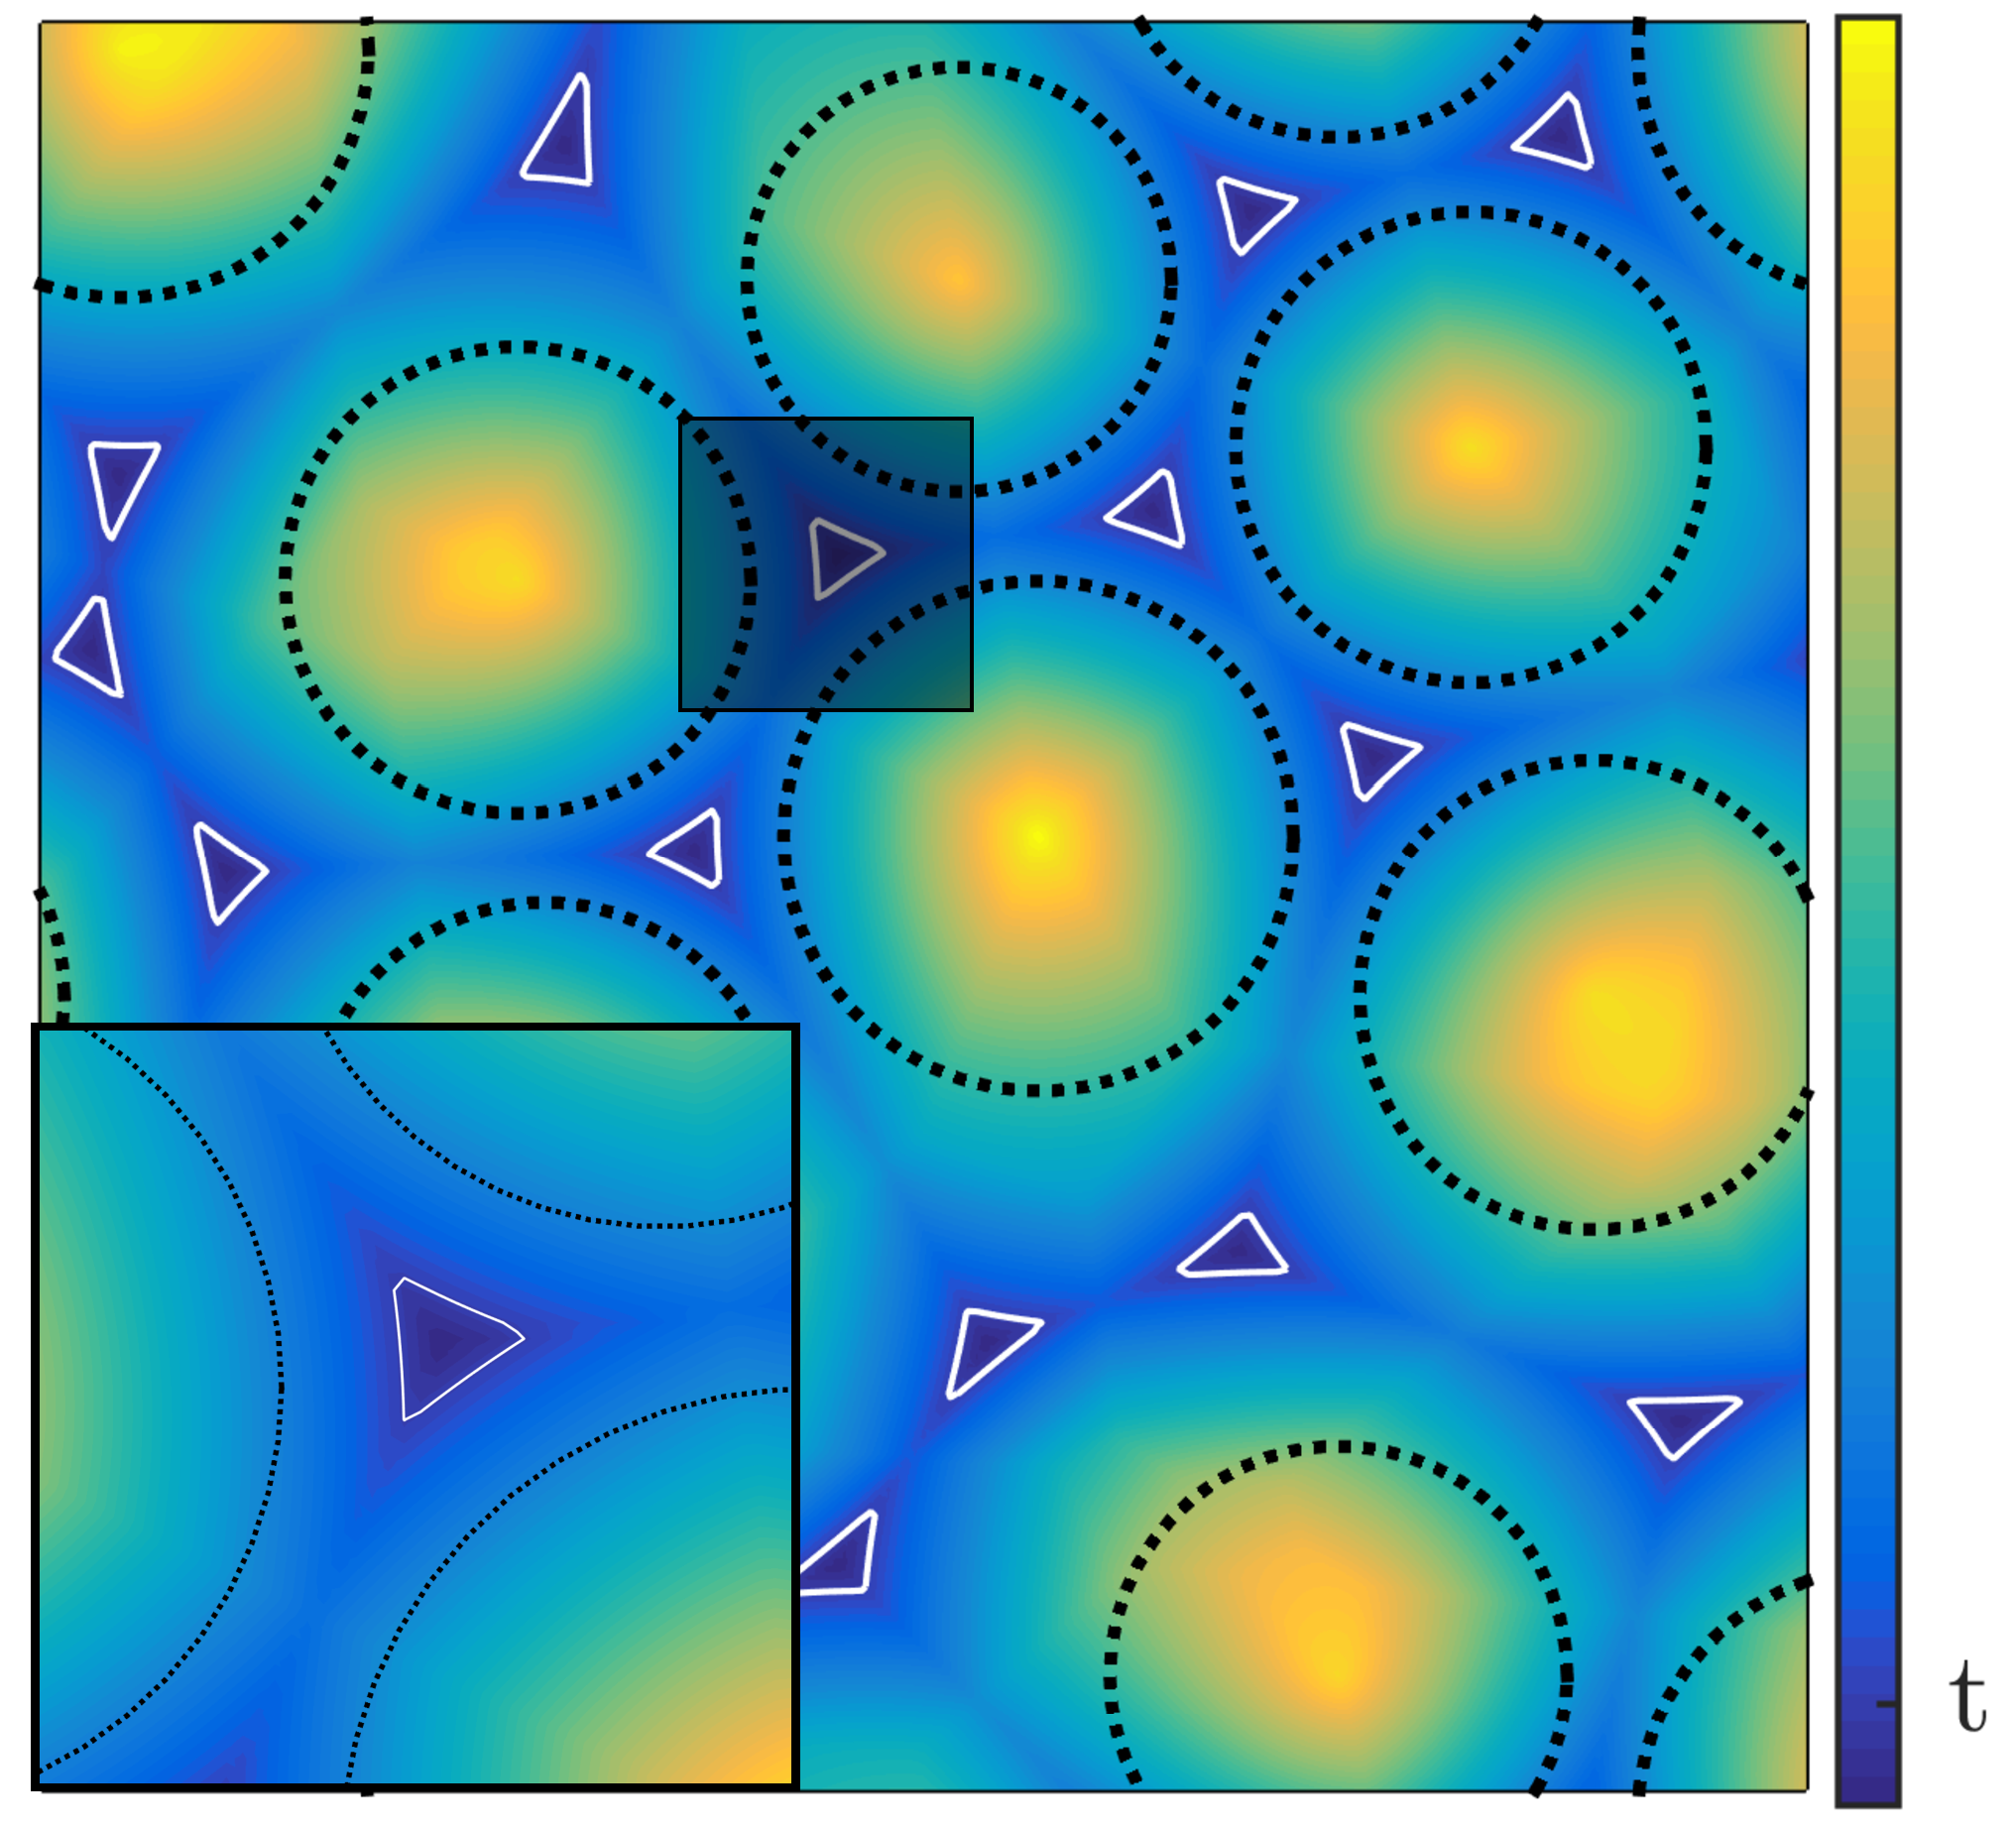
\includegraphics[width=\textwidth]{OP_Global}
		\caption{}
	\end{subfigure}
	\begin{subfigure}[b]{0.33\textwidth}
		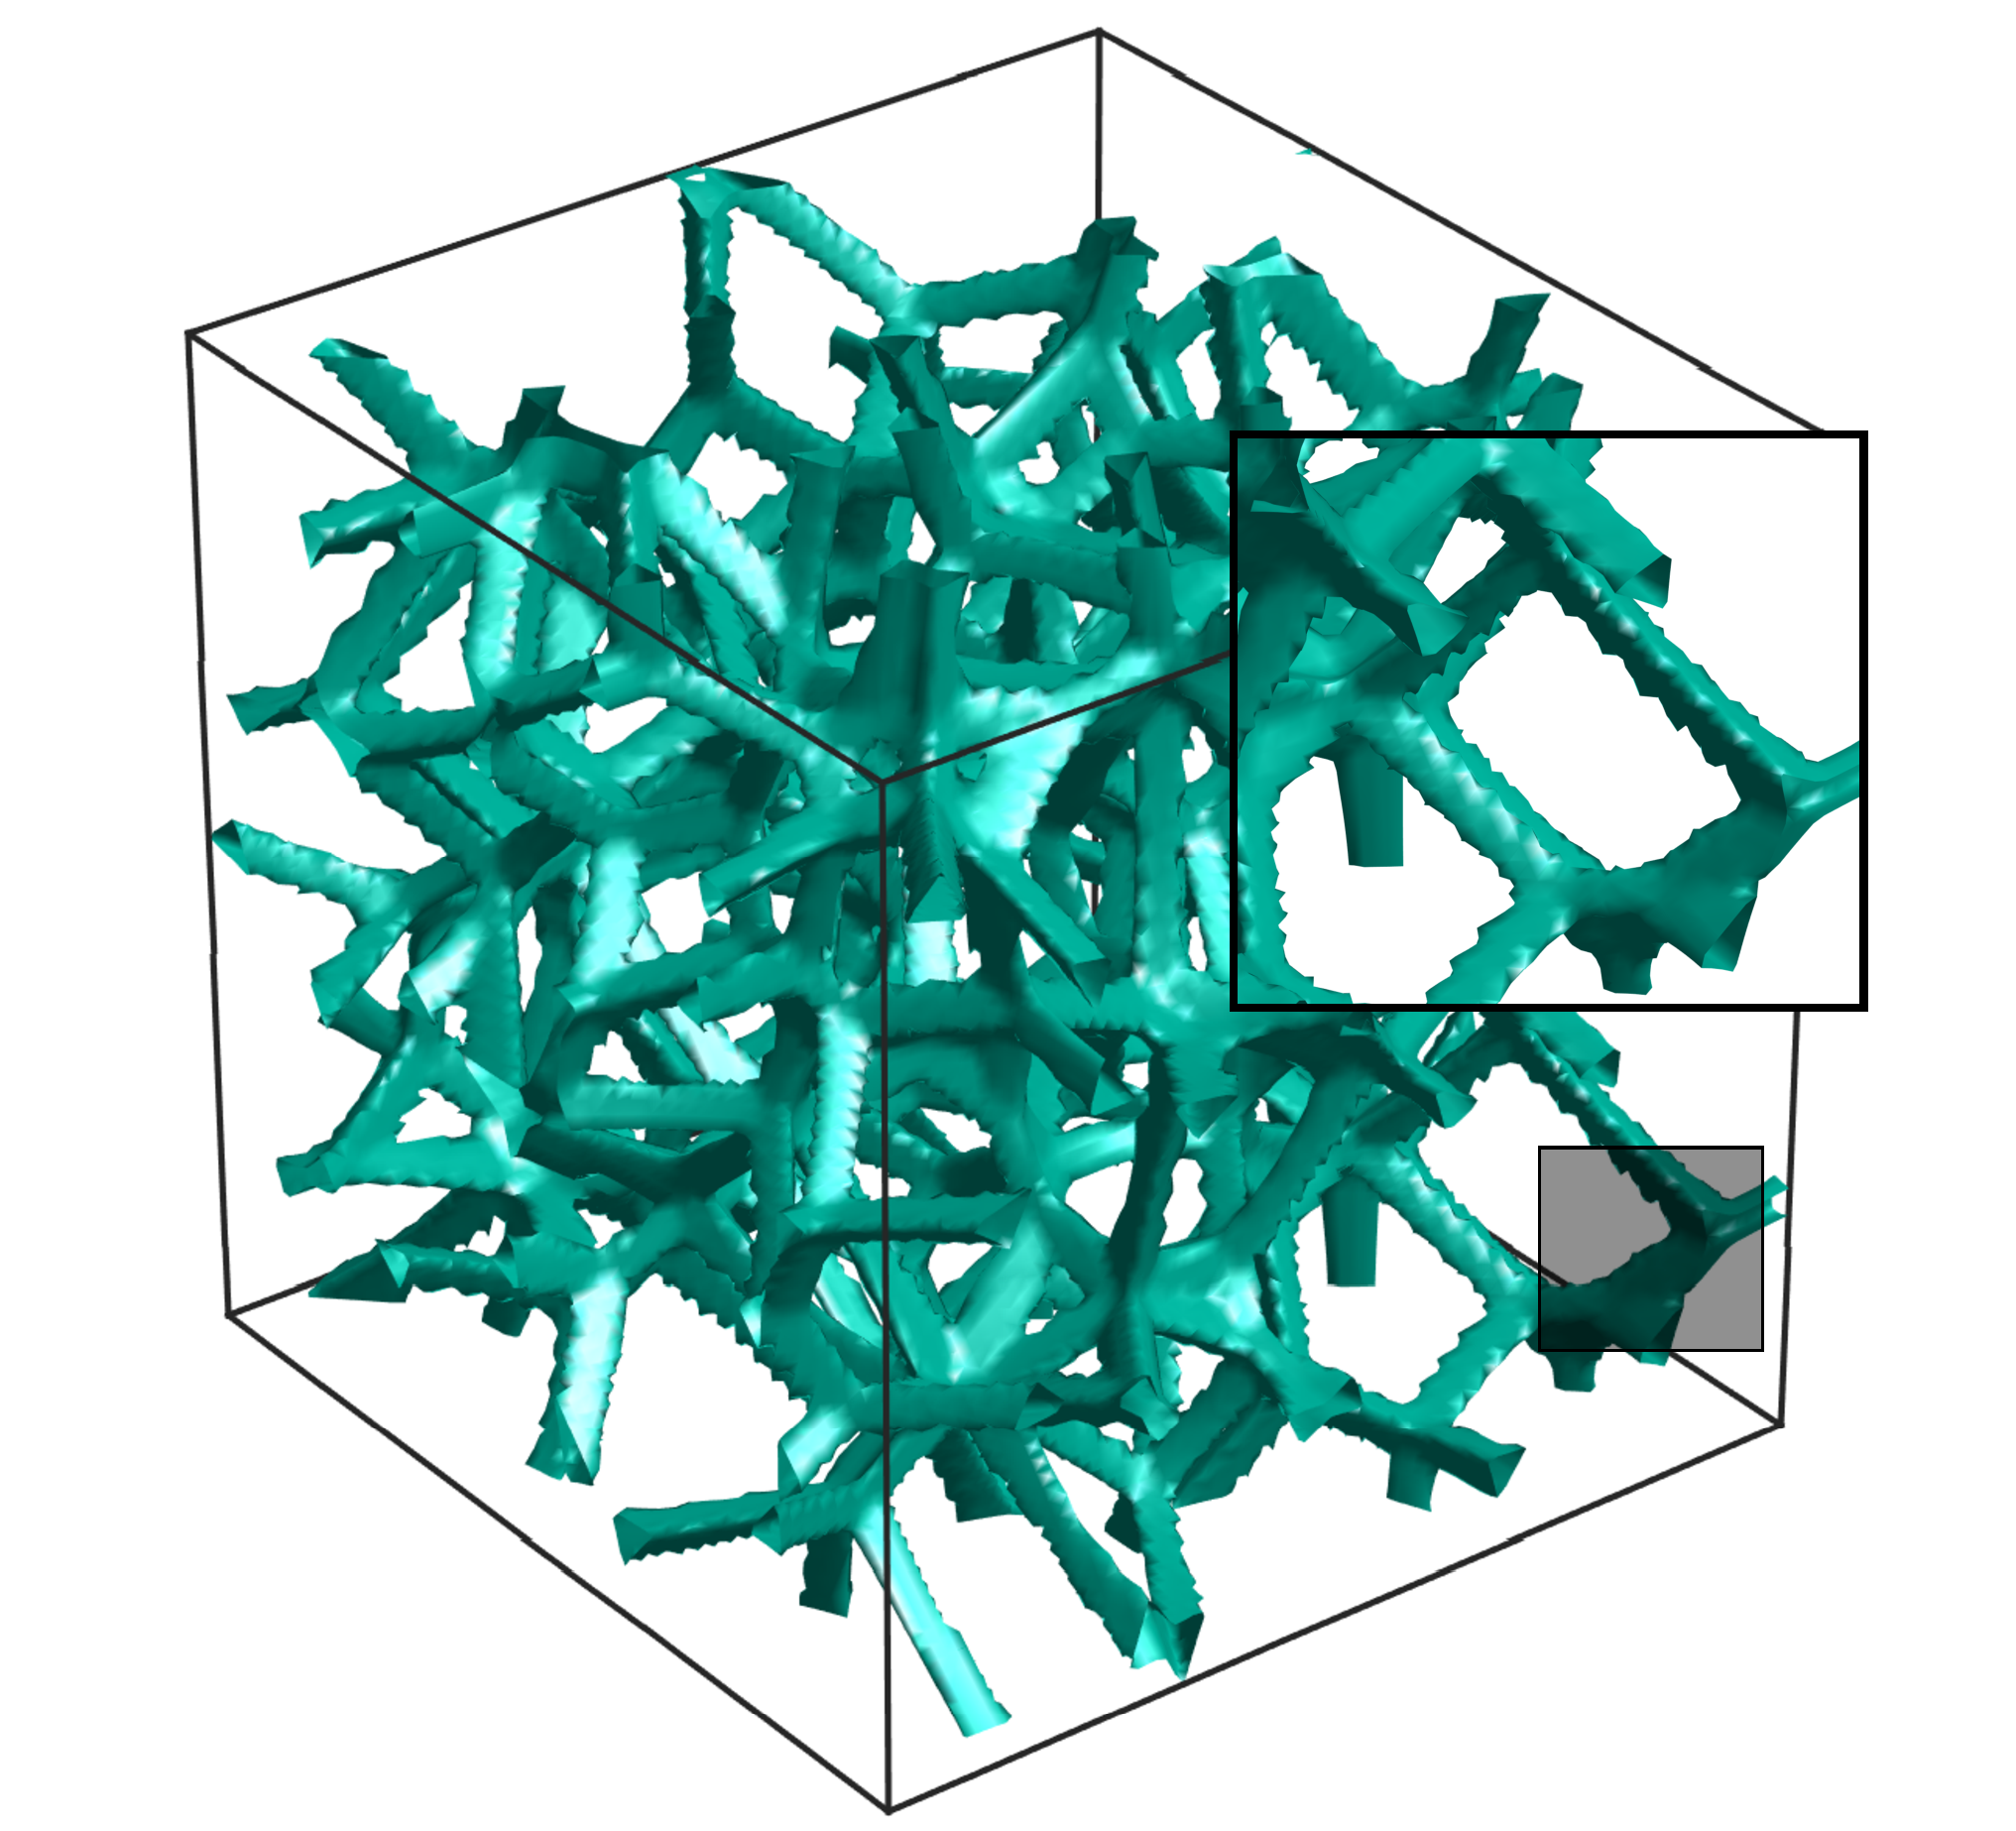
\includegraphics[width=\textwidth]{OP_3D}
		\caption{}
	\end{subfigure}
	\begin{subfigure}[b]{0.32\textwidth}
		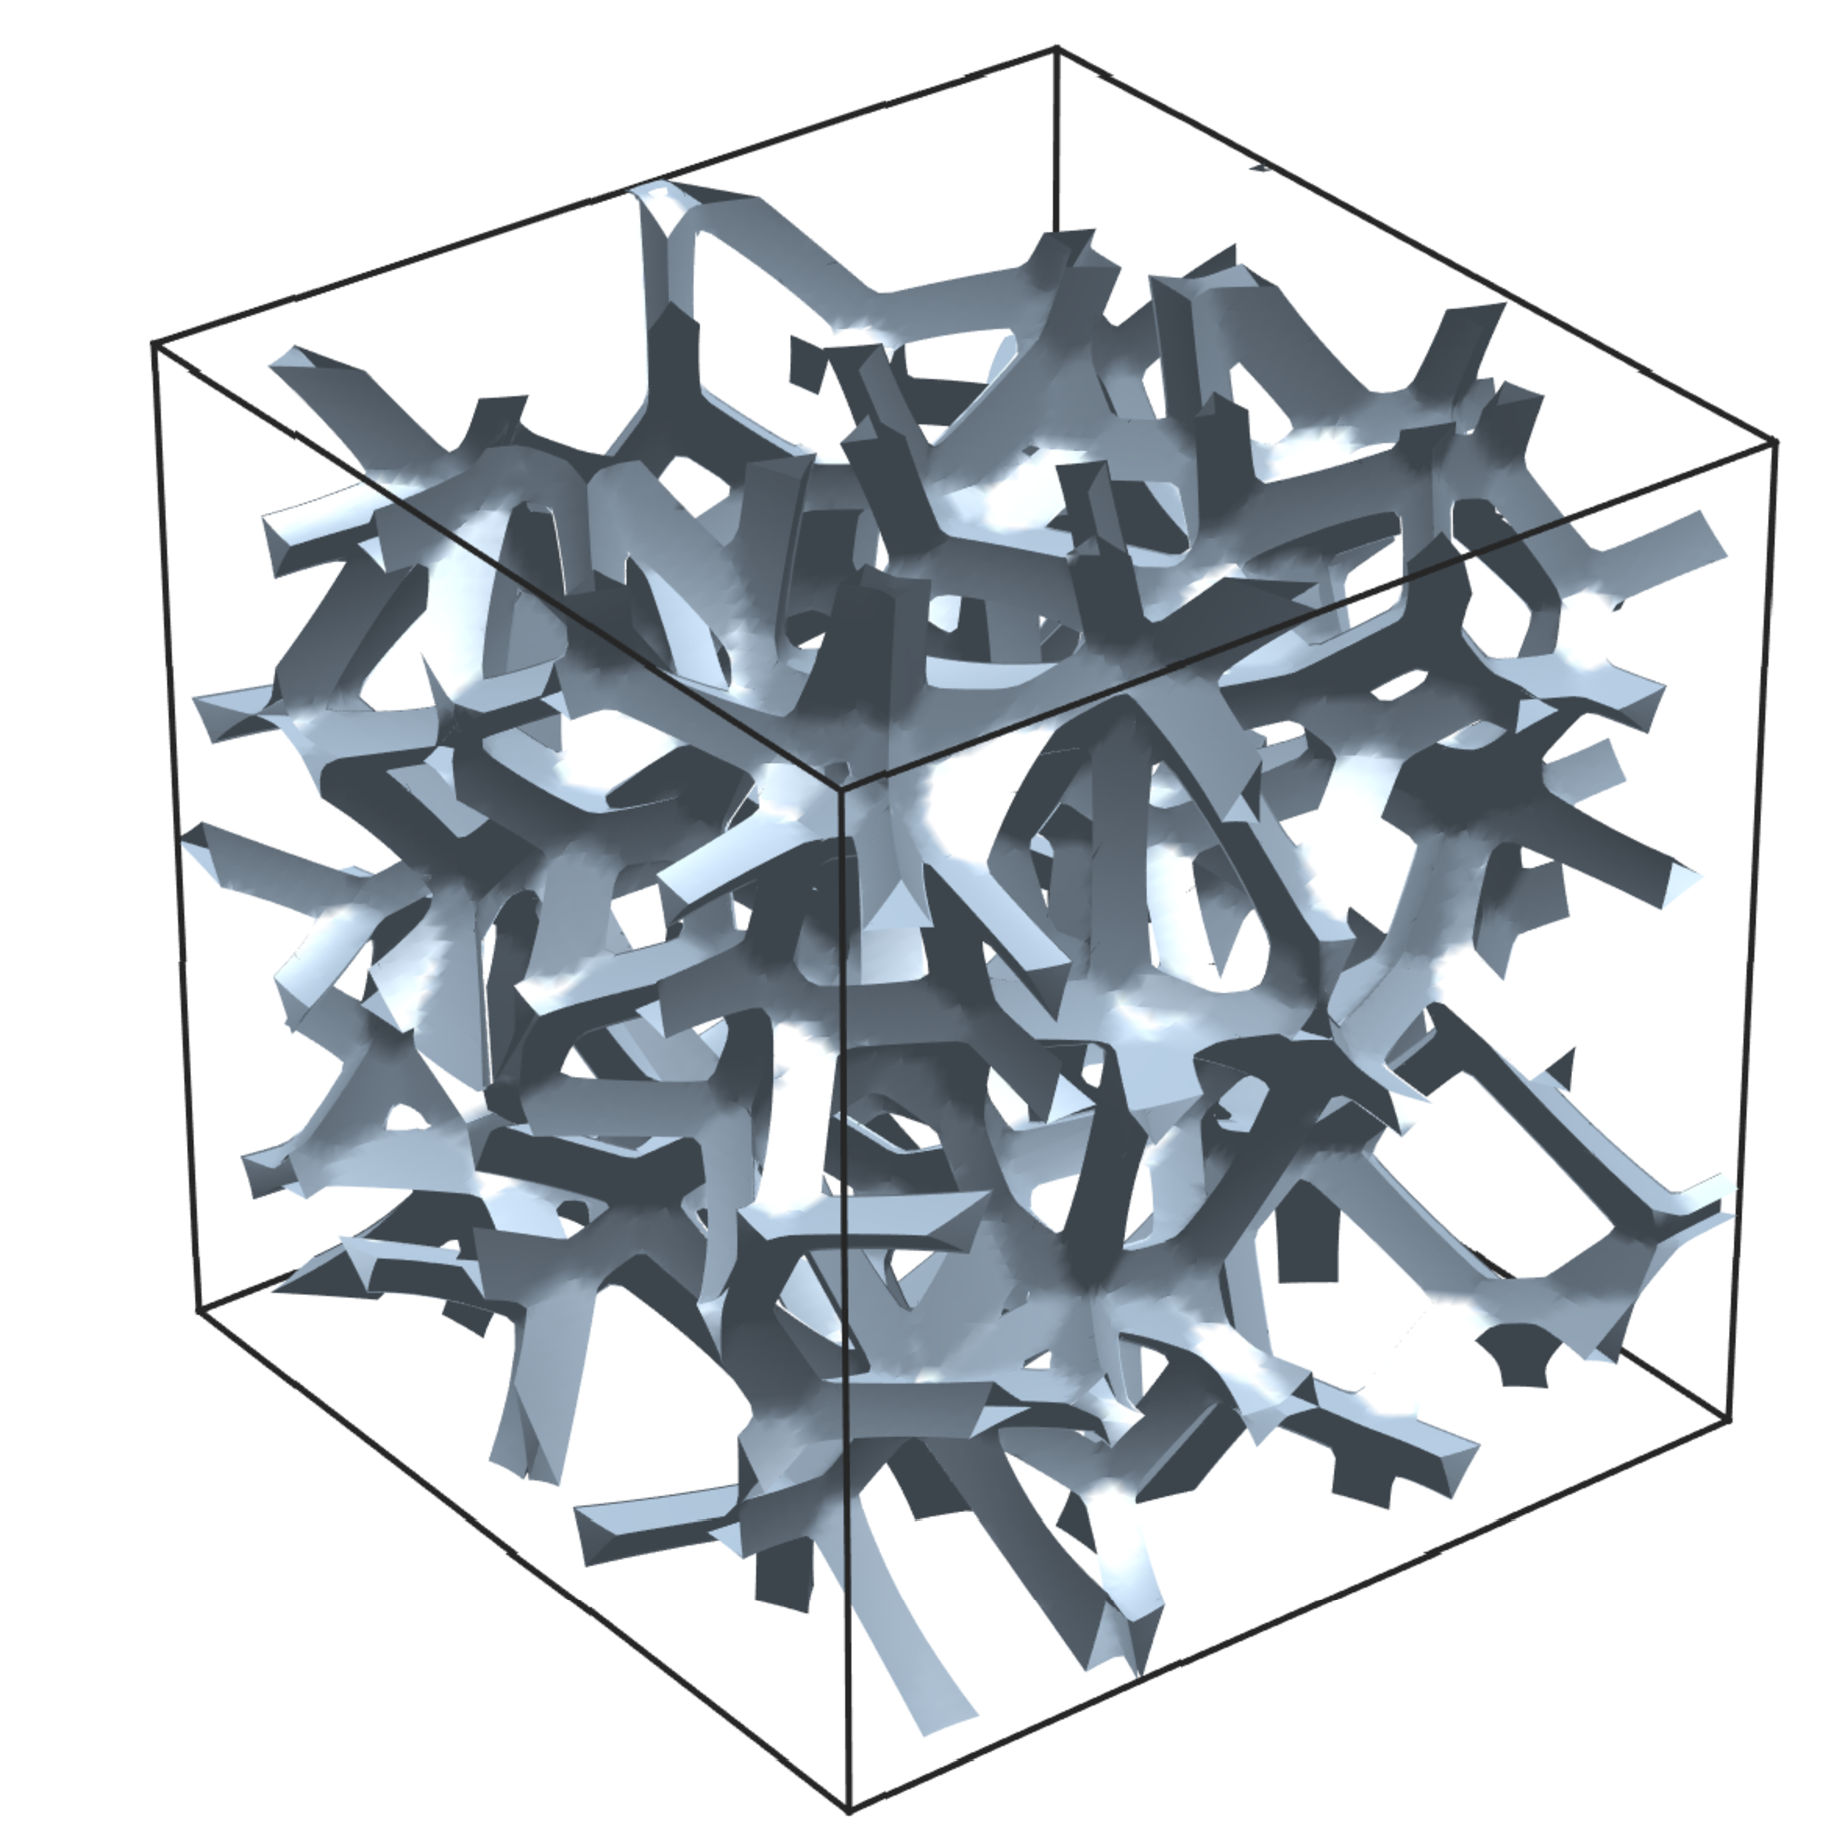
\includegraphics[width=\textwidth]{MODEL_SHARP}
		\caption{}
	\end{subfigure}
	\caption{Sharp edges extraction; Result of a single level set function extraction resulting in a blunted or jagged geometry in (a) disk packing; and (b) sphere packing using ``global" $ O_P $, and (c) result of multiple level set extraction by using ``local" $ ^IO_{Pi} $. Strut morphology variations are not implemented in this illustration. }\label{sharp1}
\end{figure}

\begin{figure}
	\centering
	\begin{subfigure}[b]{0.45\textwidth}
		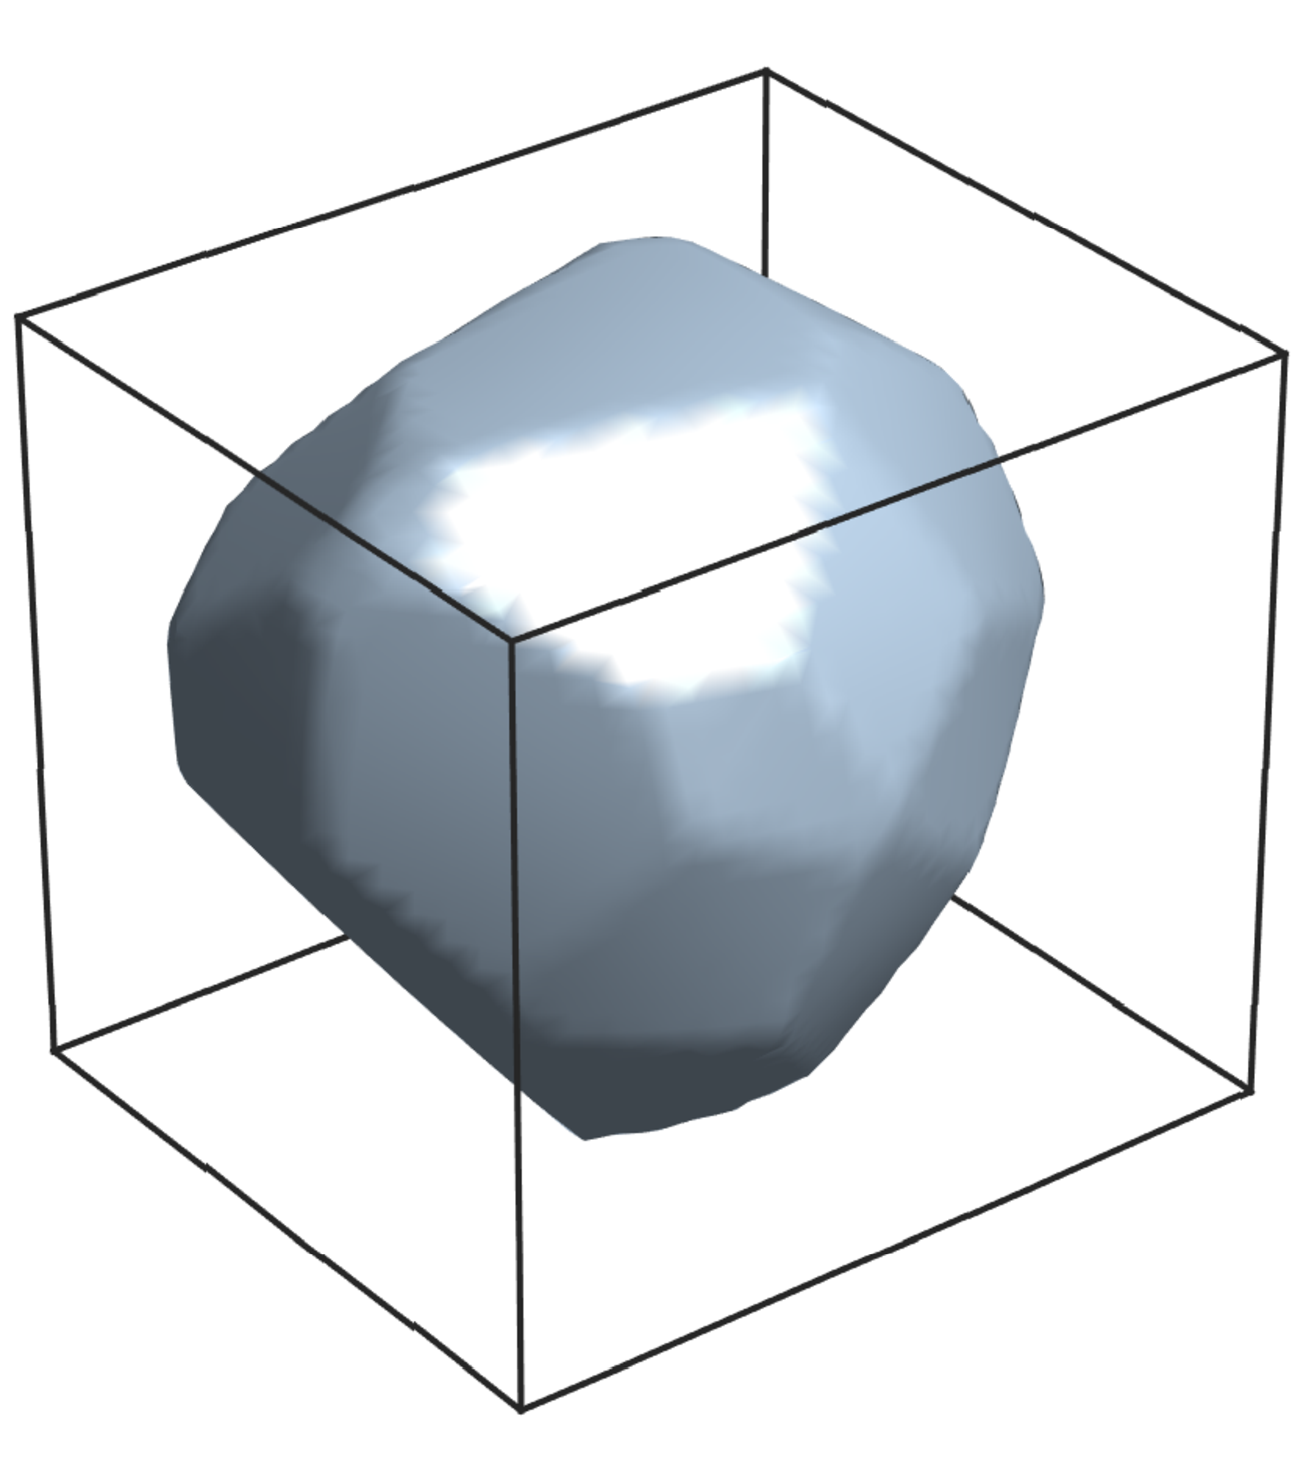
\includegraphics[width=\textwidth]{OP_INCL_9}
		\caption{}
	\end{subfigure}
	\begin{subfigure}[b]{0.45\textwidth}
		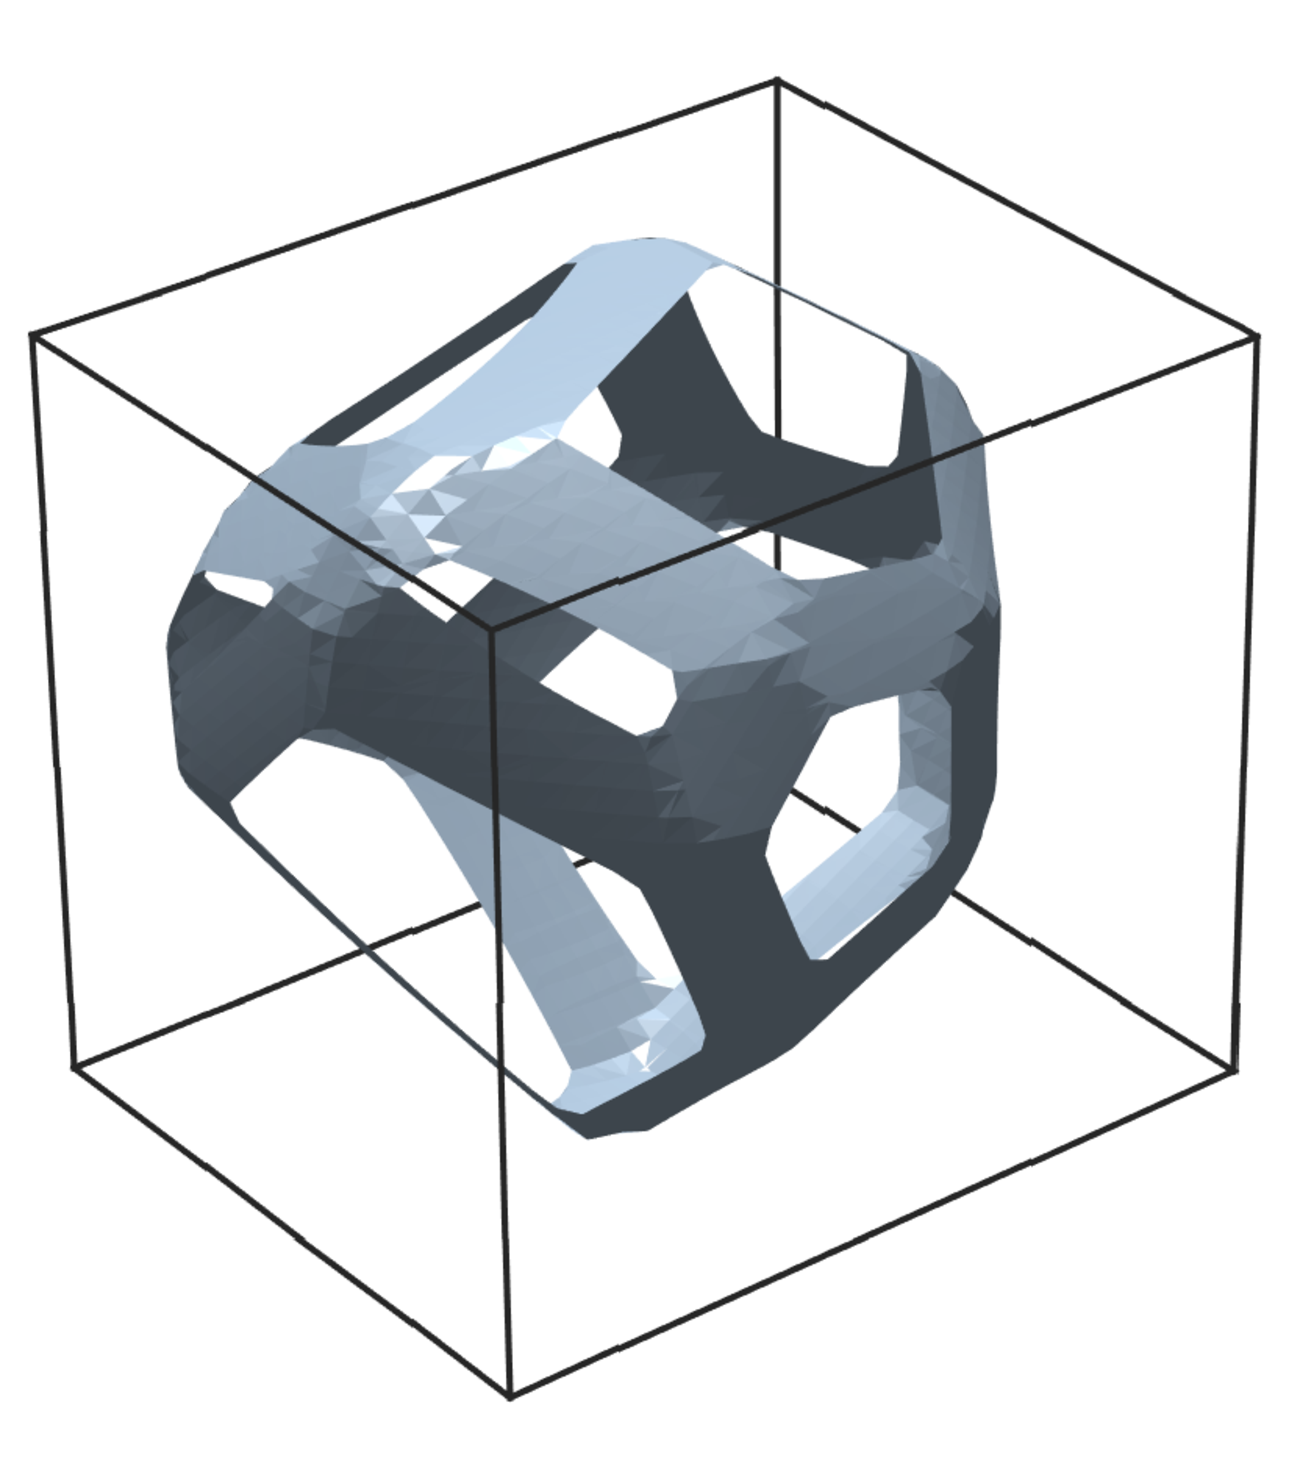
\includegraphics[width=\textwidth]{OP_INCL_9_SLICE}
		\caption{}
	\end{subfigure}
	\caption{Illustration of multiple level sets approach on a single isolated cell corresponding to an inclusion; (a) Surface resulting of the contouring of the ``local" level set function $ ^IO_{Pi} $, and (b) surface after slicing by the ``local'' level set functions of the neighboring inclusions.}\label{sharp2}
\end{figure}
To achieve this enhanced slicing, a ``local" level set function for each inclusion is built by modifying the ``global" $ DN_k $ functions, and is further denoted as $ ^I DN_{ki} $. Without changing the definition of $ O_P $, a ``local" $ ^IO_{Pi} $ is built with $ ^I DN_{ki} $ using Eq. (\ref{OP}). This ``local" level set is used to extract the surface coming from the considered inclusion, while similarly built ``local" level sets for the neighboring inclusions are used to perform the slicing operation. Being \textit{ad-hoc} functions, the local $ ^I DN_{ki} $ functions are constrained to be equal to their global counterparts inside $ ^I \Theta_i $ and $ C^1 $ continuous across the boundary $ \Phi_{\Theta i} $. The values of the local function inside $ ^I \Theta_i $ are intended to yield the same results as their global counterparts while the values in $ ^O \Theta_i $ do not matter as they will be sliced off. However, in order to enable proper contouring, the surface has to be smooth on $ \Phi_{\Theta i} $. 

The values of the local $ ^IO_{Pi} $ can be obtained by a simple reorganization of the $ DN_k $ functions, which consist of assemblies of patches coming from $ DS_i $. This reorganization can be achieved keeping in mind the aforementioned constraints necessary to construct $ ^IO_{Pi} $:
\begin{subequations}
	\begin{equation}
	^IDN_{1i}=DS_i(\textbf{x})\label{inner1},
	\end{equation}
	\begin{equation}
	^IDN_{2i}=\begin{cases}
	  DN_2(\textbf{x})\text{ where }NN_2(\textbf{x})\ne i,
	\\DN_1(\textbf{x})\text{ where }NN_2(\textbf{x})= i\label{inner2},
	\end{cases}
	\end{equation}
	\begin{equation}
	^IDN_{3i}(\textbf{x})=DN_3(\textbf{x})\label{inner3}.
	\end{equation}
\end{subequations}

Eqs. (\ref{inner1}) and (\ref{inner2}) are illustrated in Figures \ref{inner4}a and \ref{inner4}b, respectively. Figure \ref{inner4}c illustrates the extraction of the triangular slices using ``local" $ t $ level sets of adjacent inclusions. Eq. (\ref{inner3}) can be used as $ DN_3 $ is already $ C^1 $ continuous across $ \Phi_{\Theta i} $. Further discussions on the extraction of these functions can be found in appendix of \cite{sononAdvancedApproachGeneration2015}. To avoid the memory requirements linked to the storage of the ``local" functions of all inclusions, these functions can be constructed in a simple and efficient manner using indexed operations whenever a particular surface from an inclusion needs to be treated, even for large RVEs with a large number of inclusions.

\begin{figure}
	\centering
	\begin{subfigure}[b]{0.32\textwidth}
		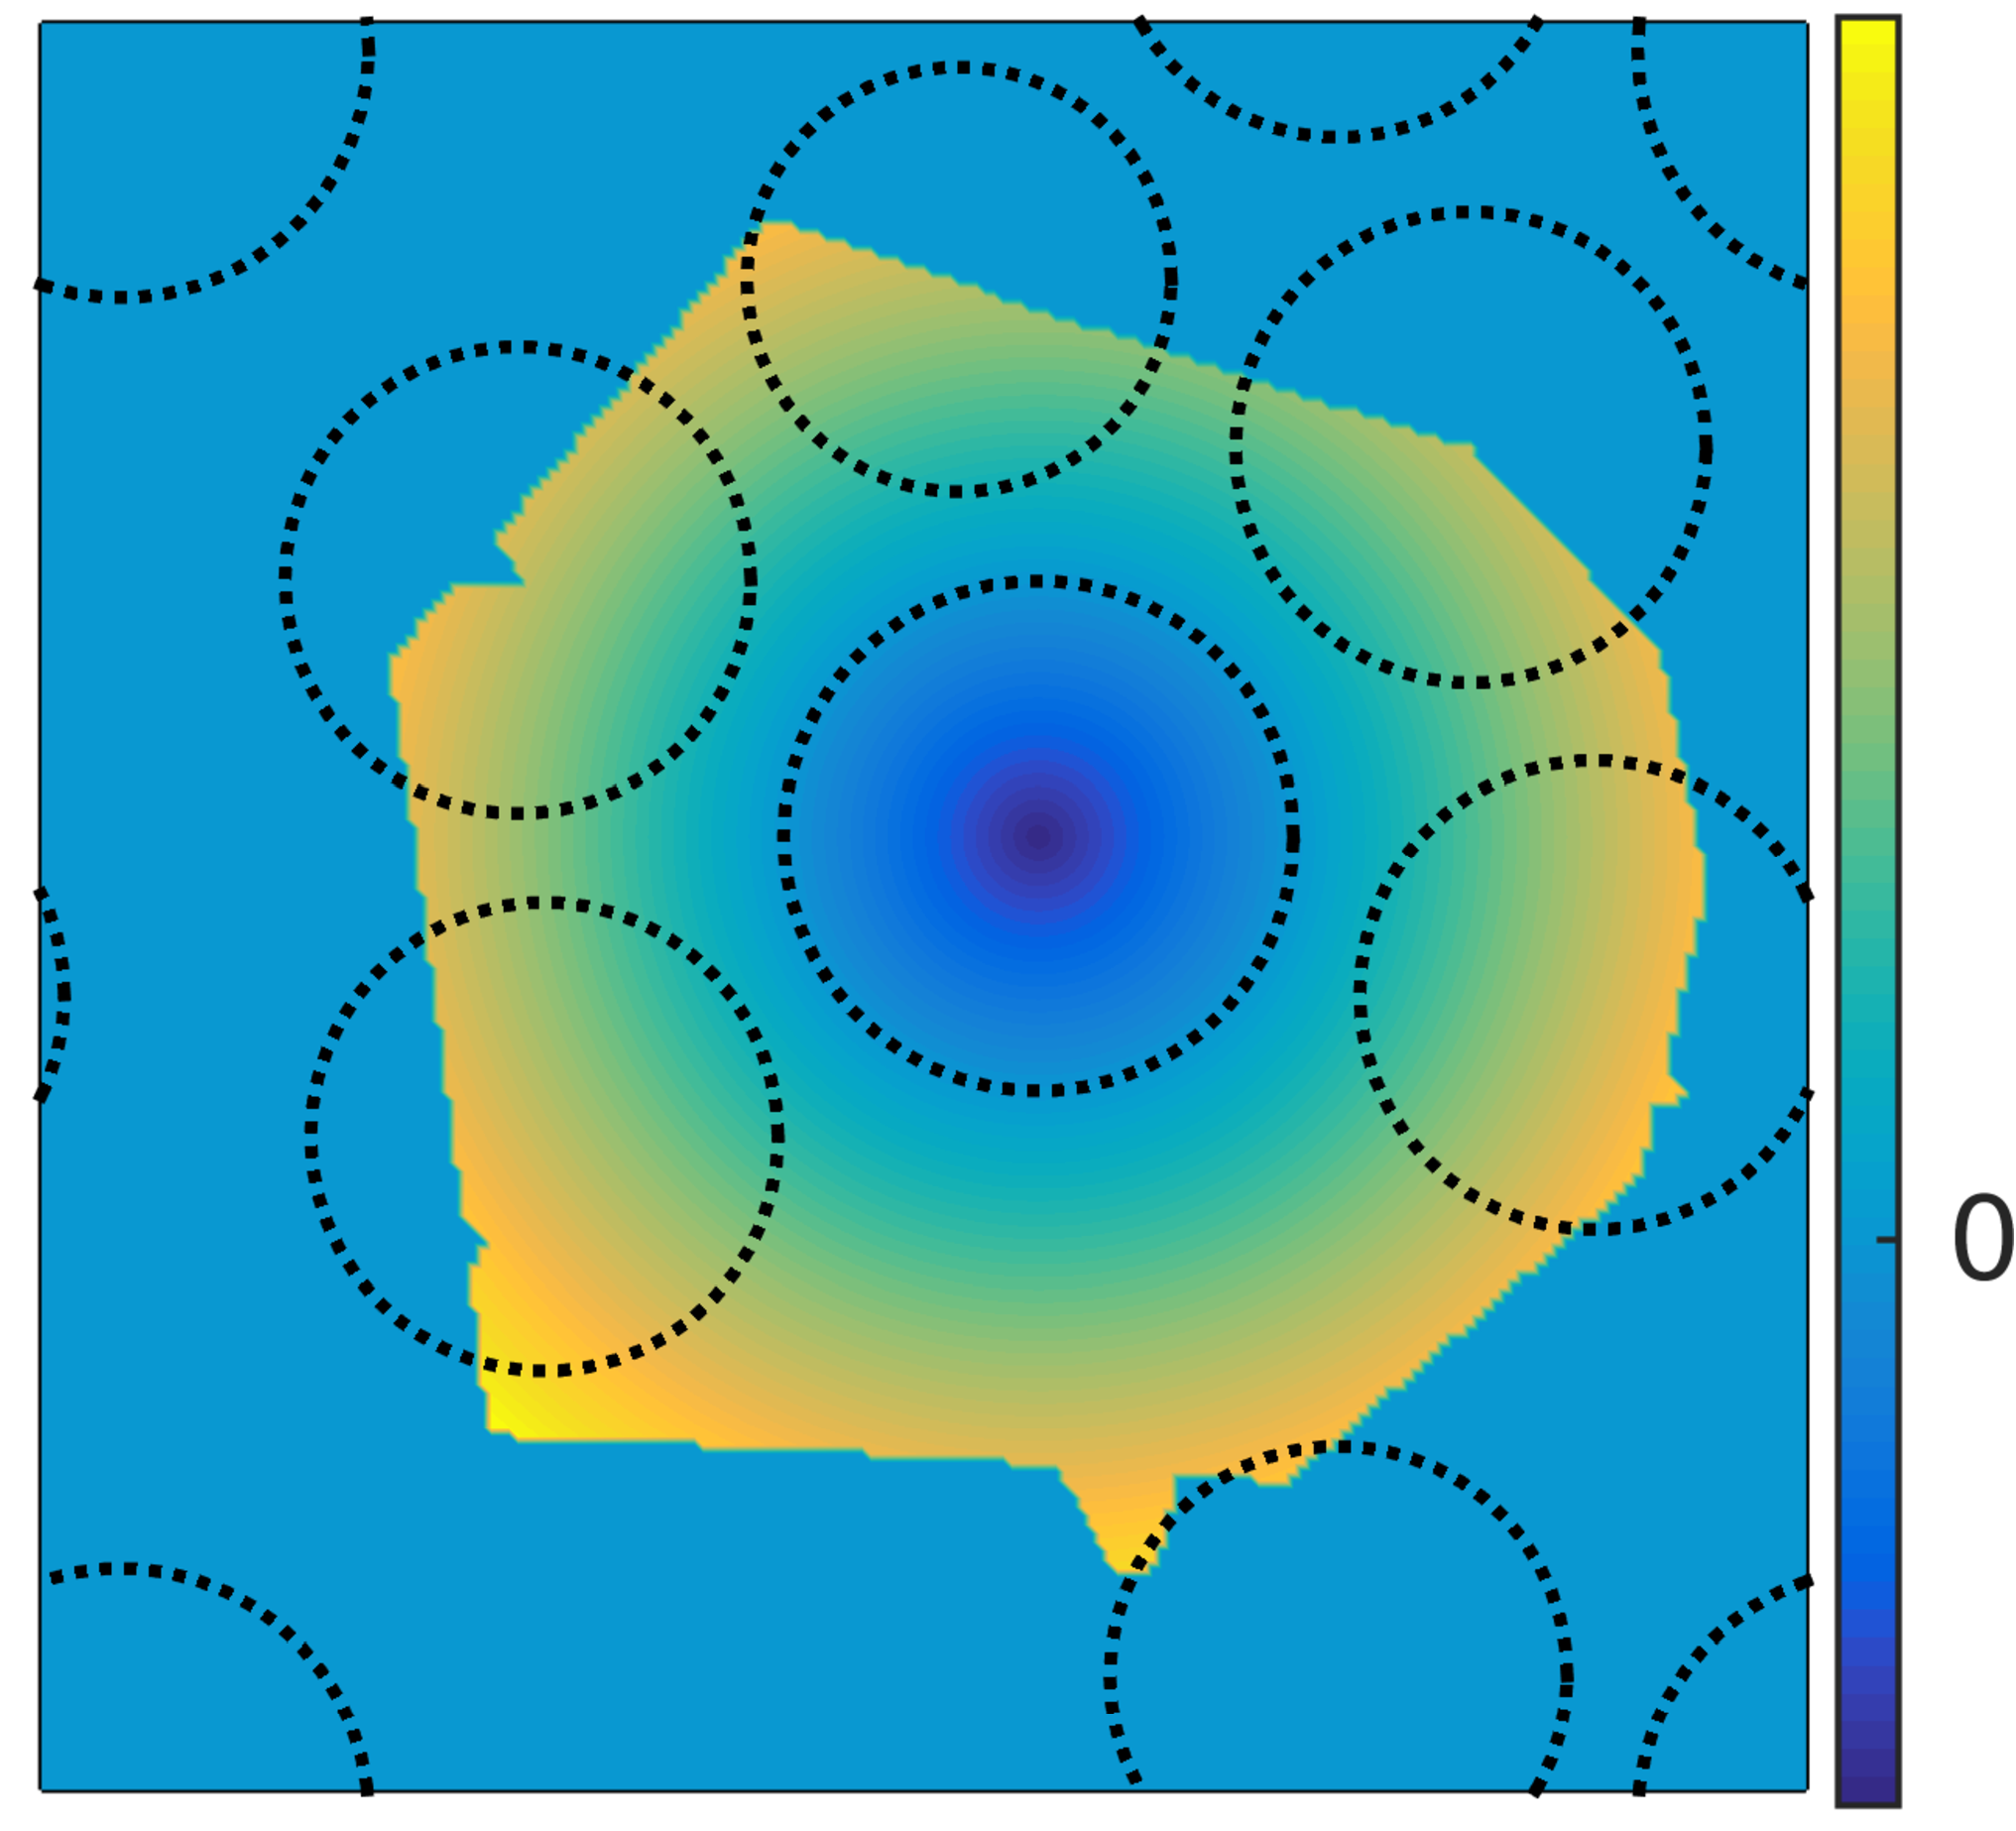
\includegraphics[width=\textwidth]{I_DN1}
		\caption{}
	\end{subfigure}
	\begin{subfigure}[b]{0.32\textwidth}
		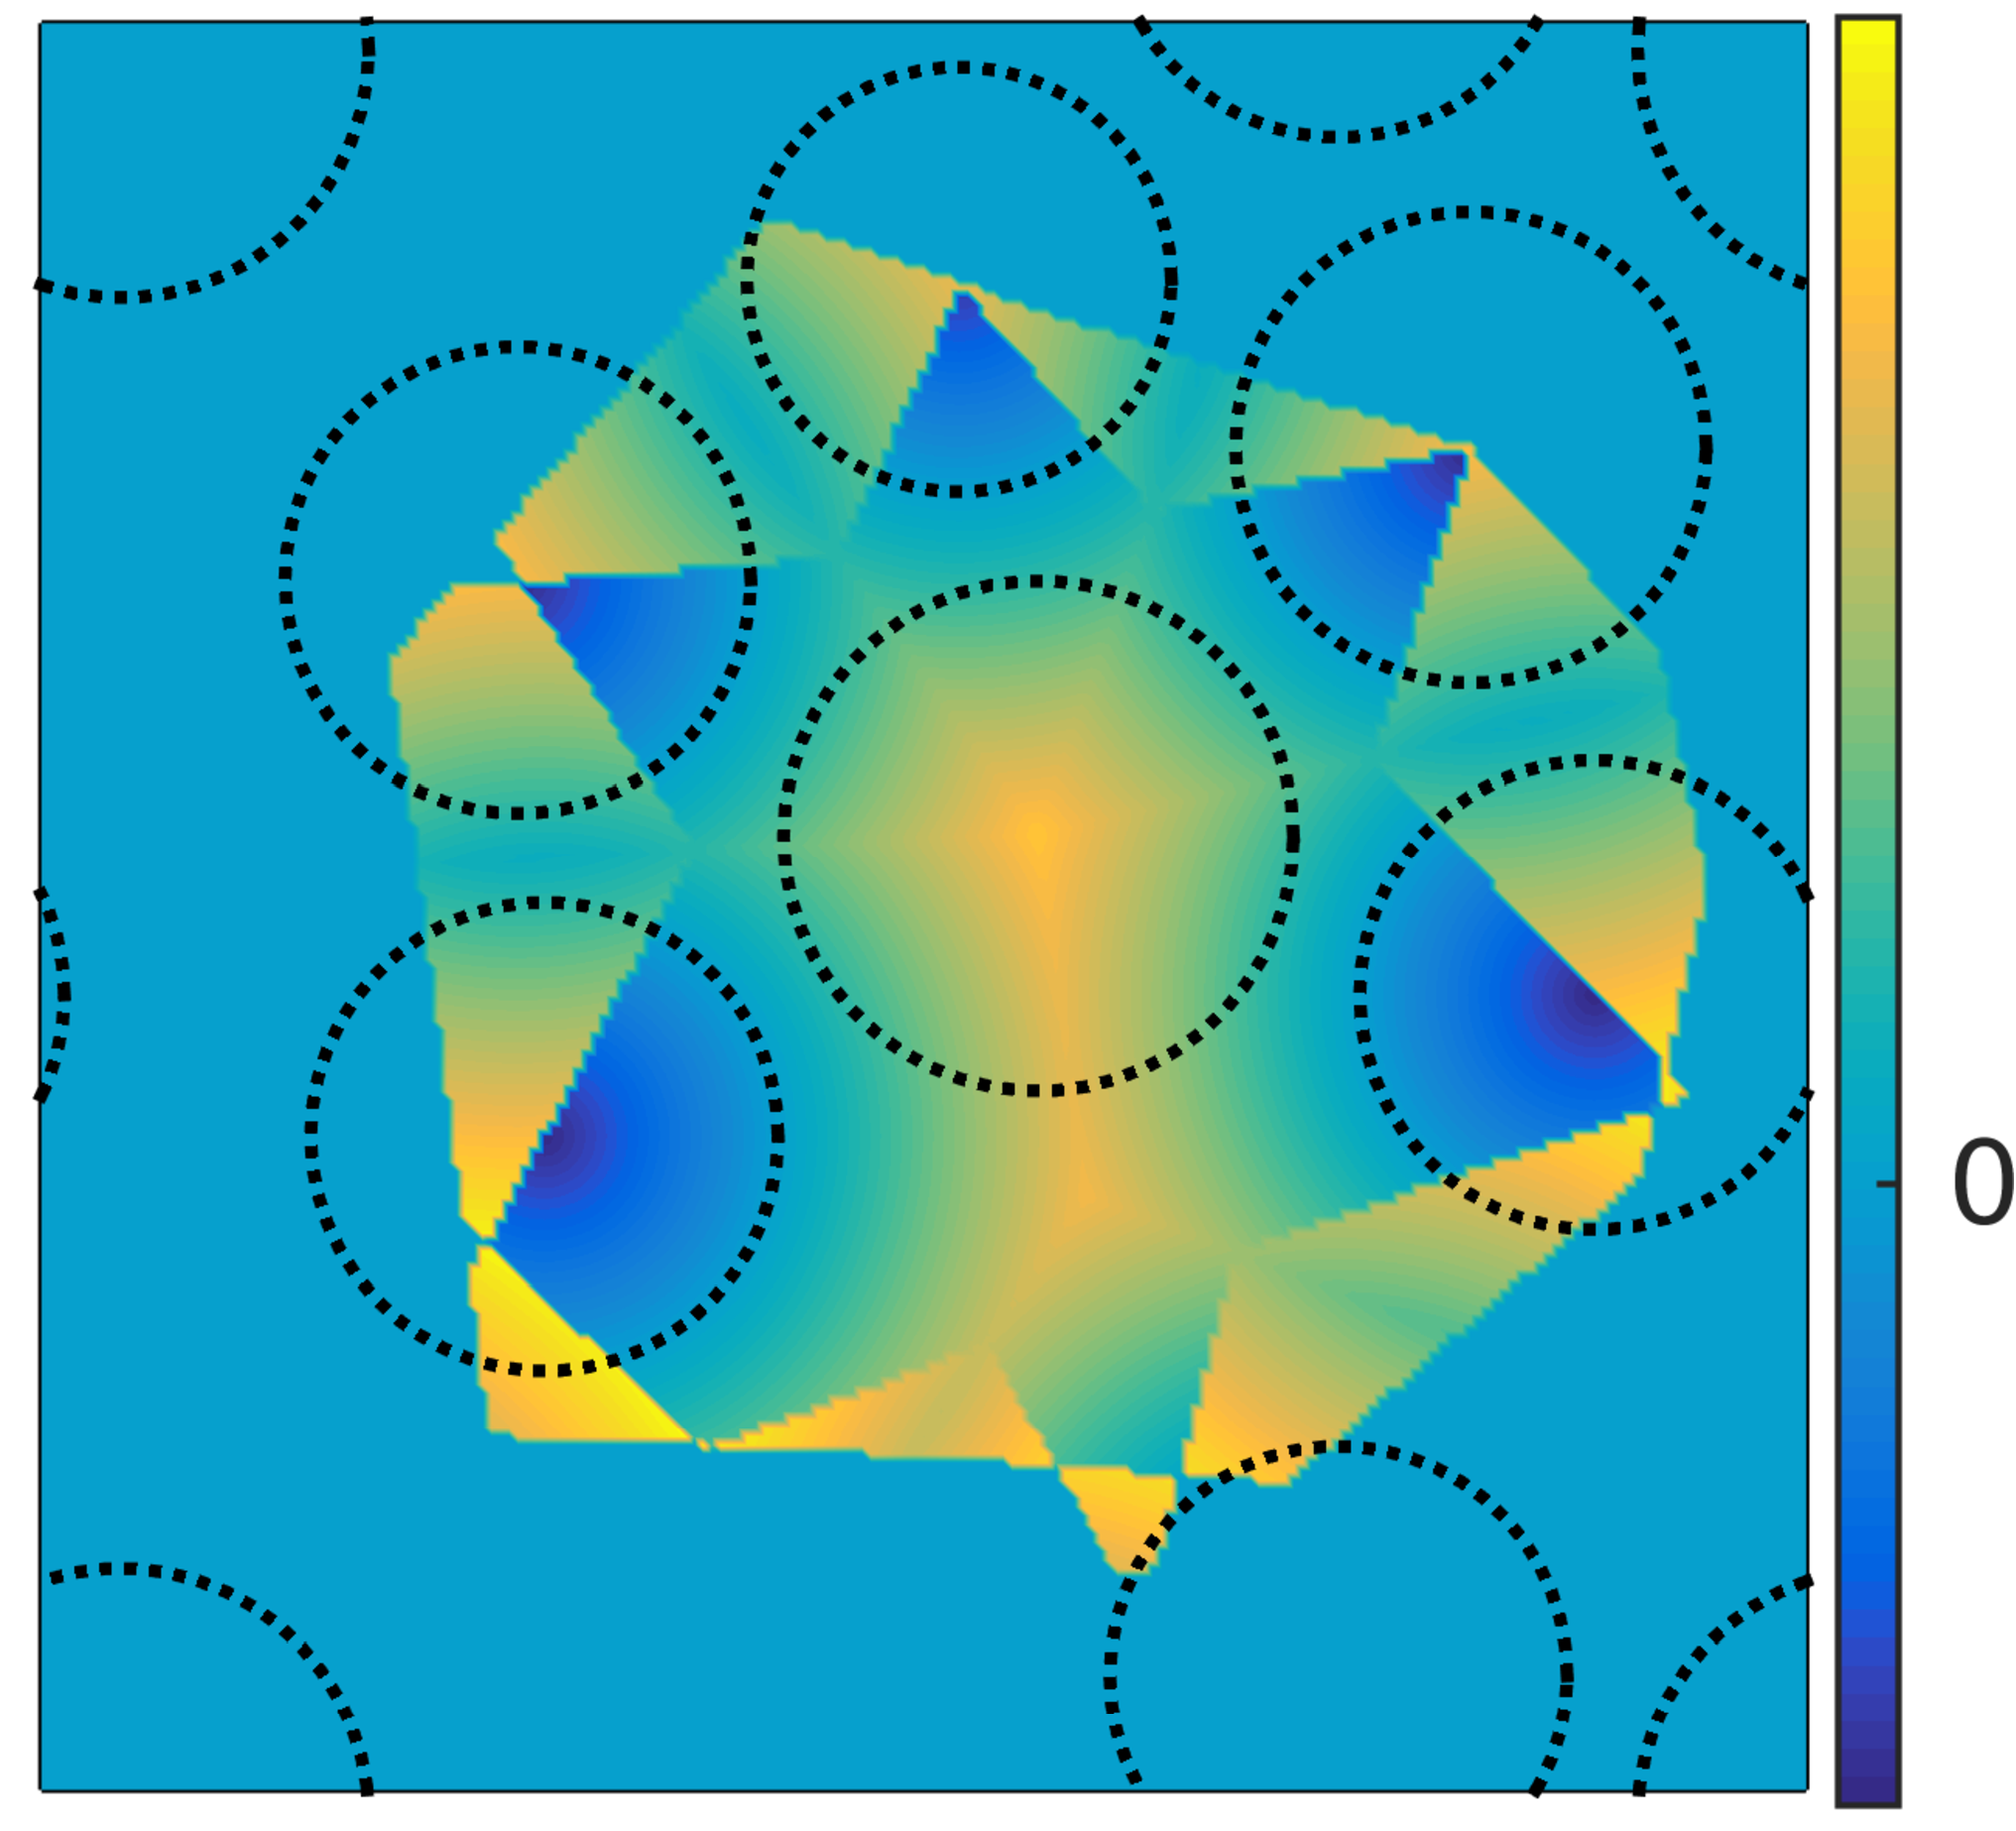
\includegraphics[width=\textwidth]{I_DN2}
		\caption{}
	\end{subfigure}
	\begin{subfigure}[b]{0.32\textwidth}
		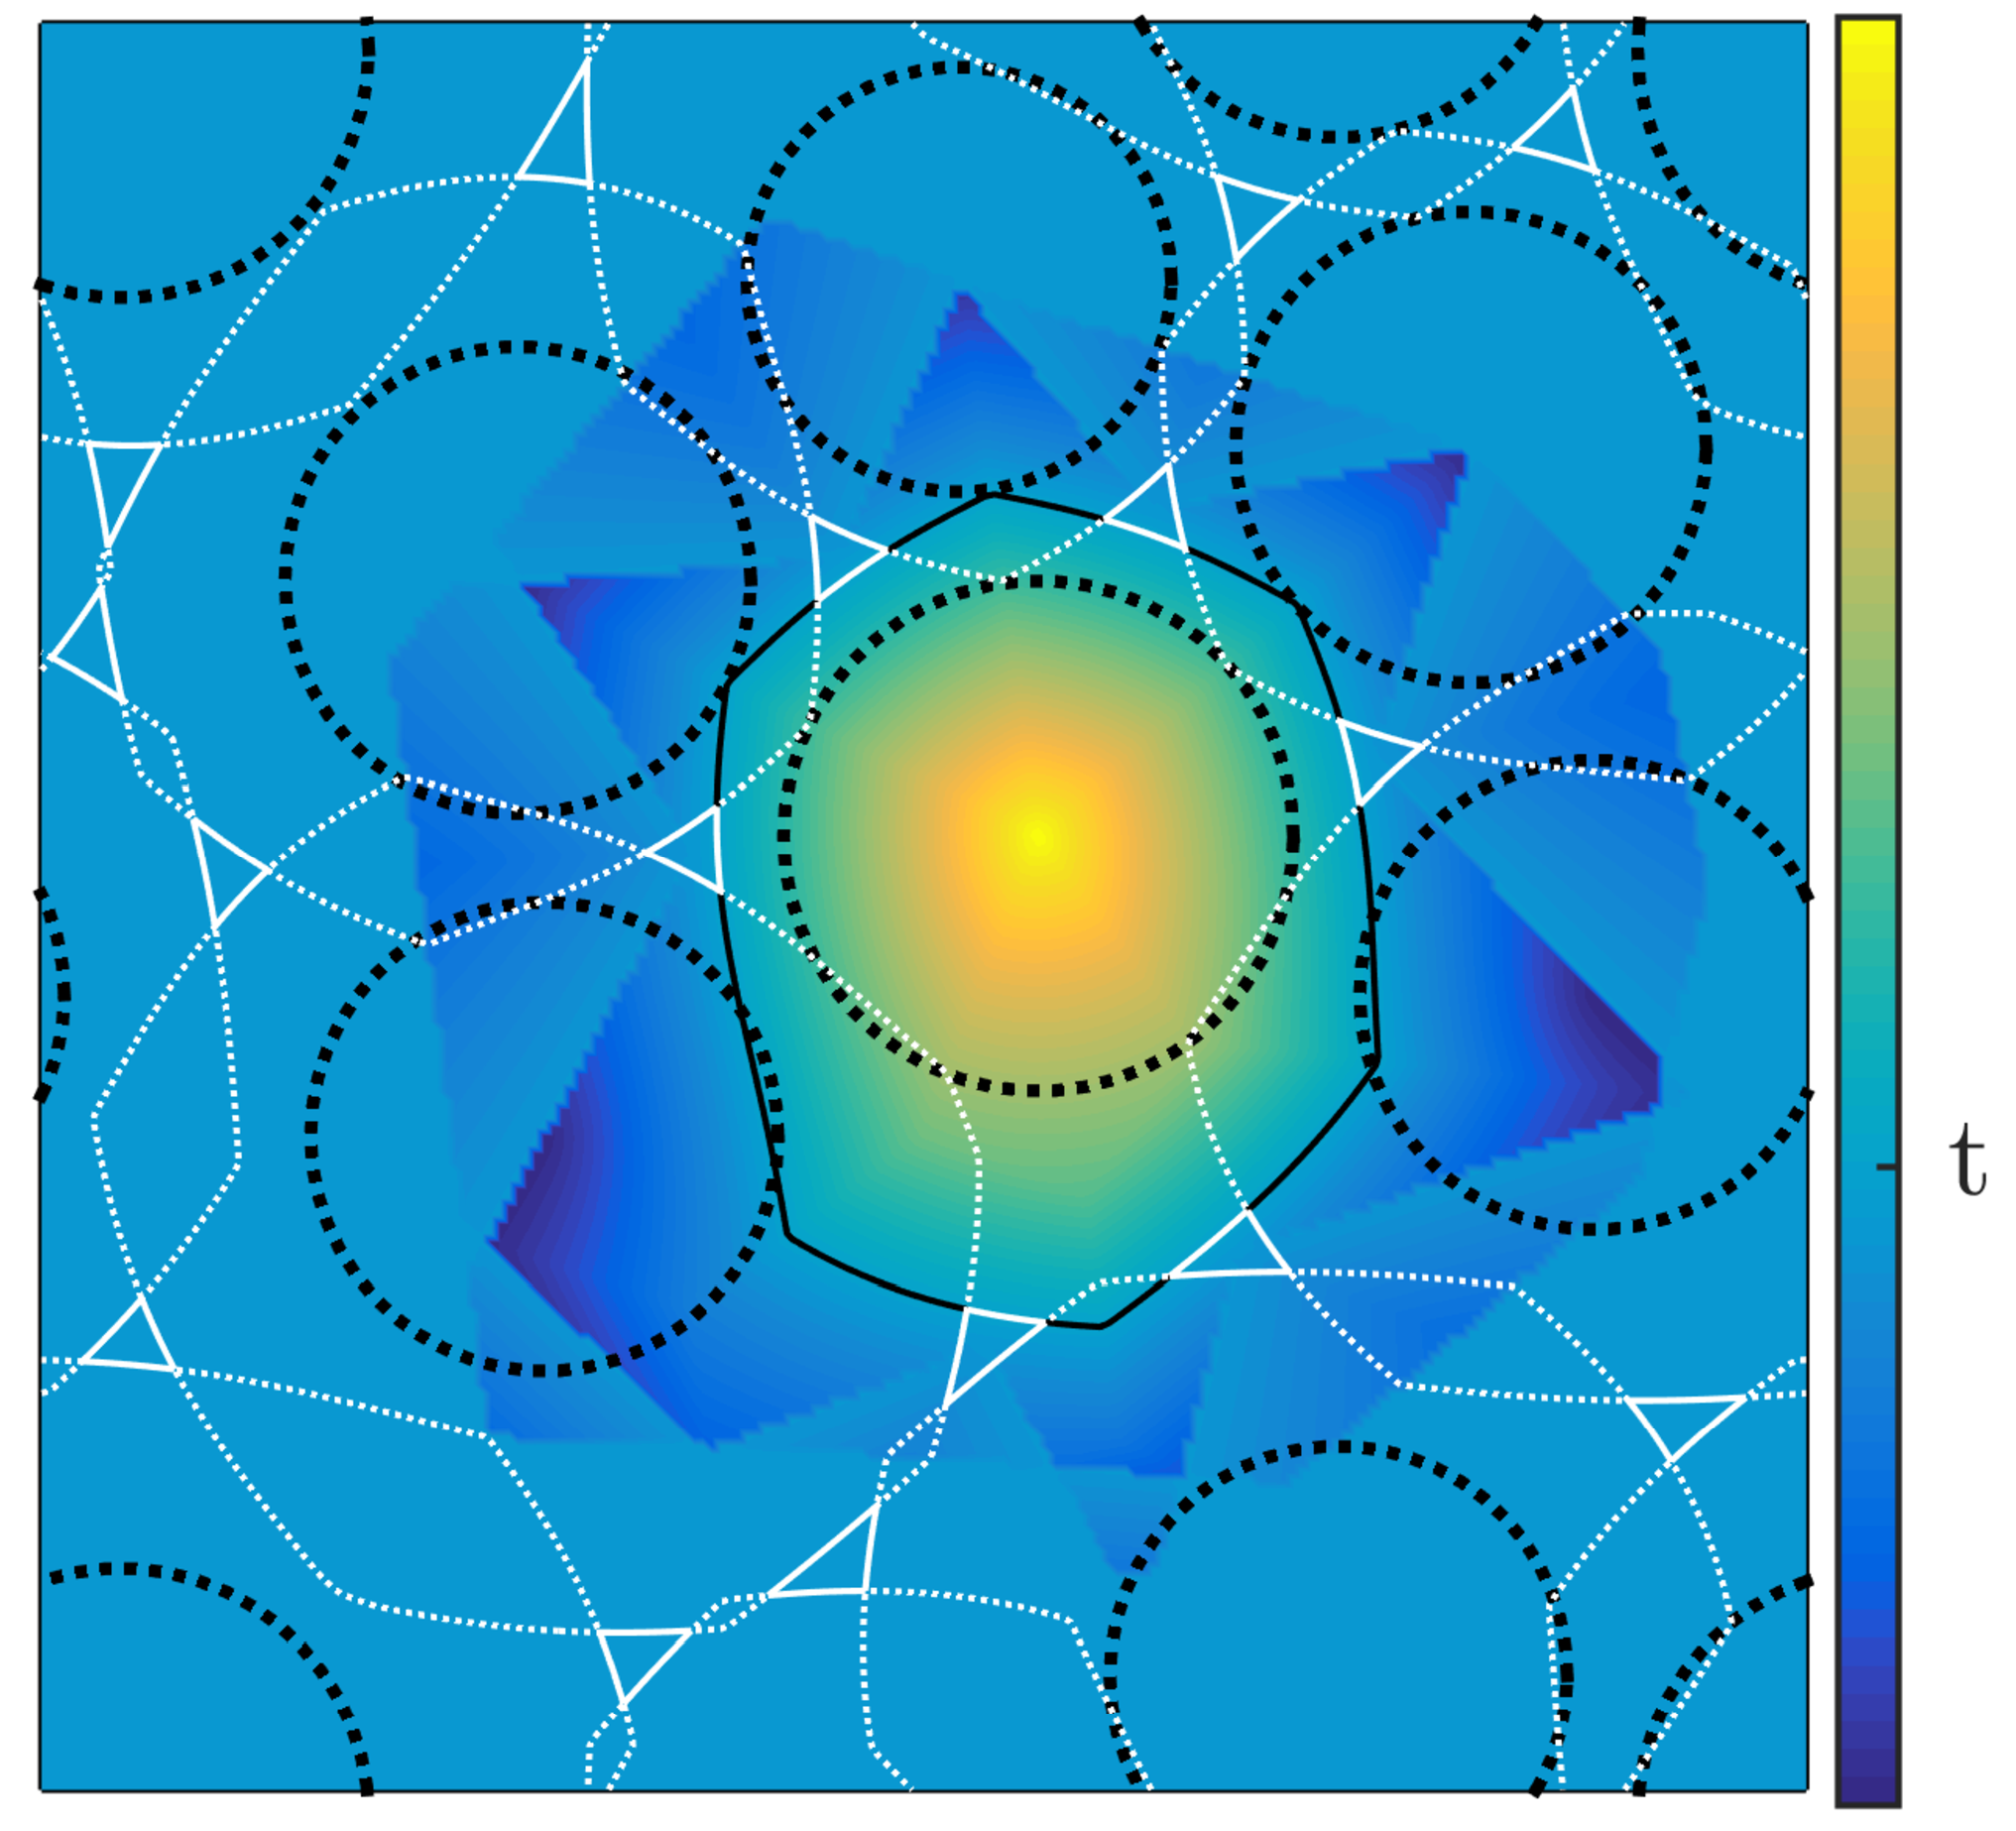
\includegraphics[width=\textwidth]{I_OP}
		\caption{}
	\end{subfigure}
%	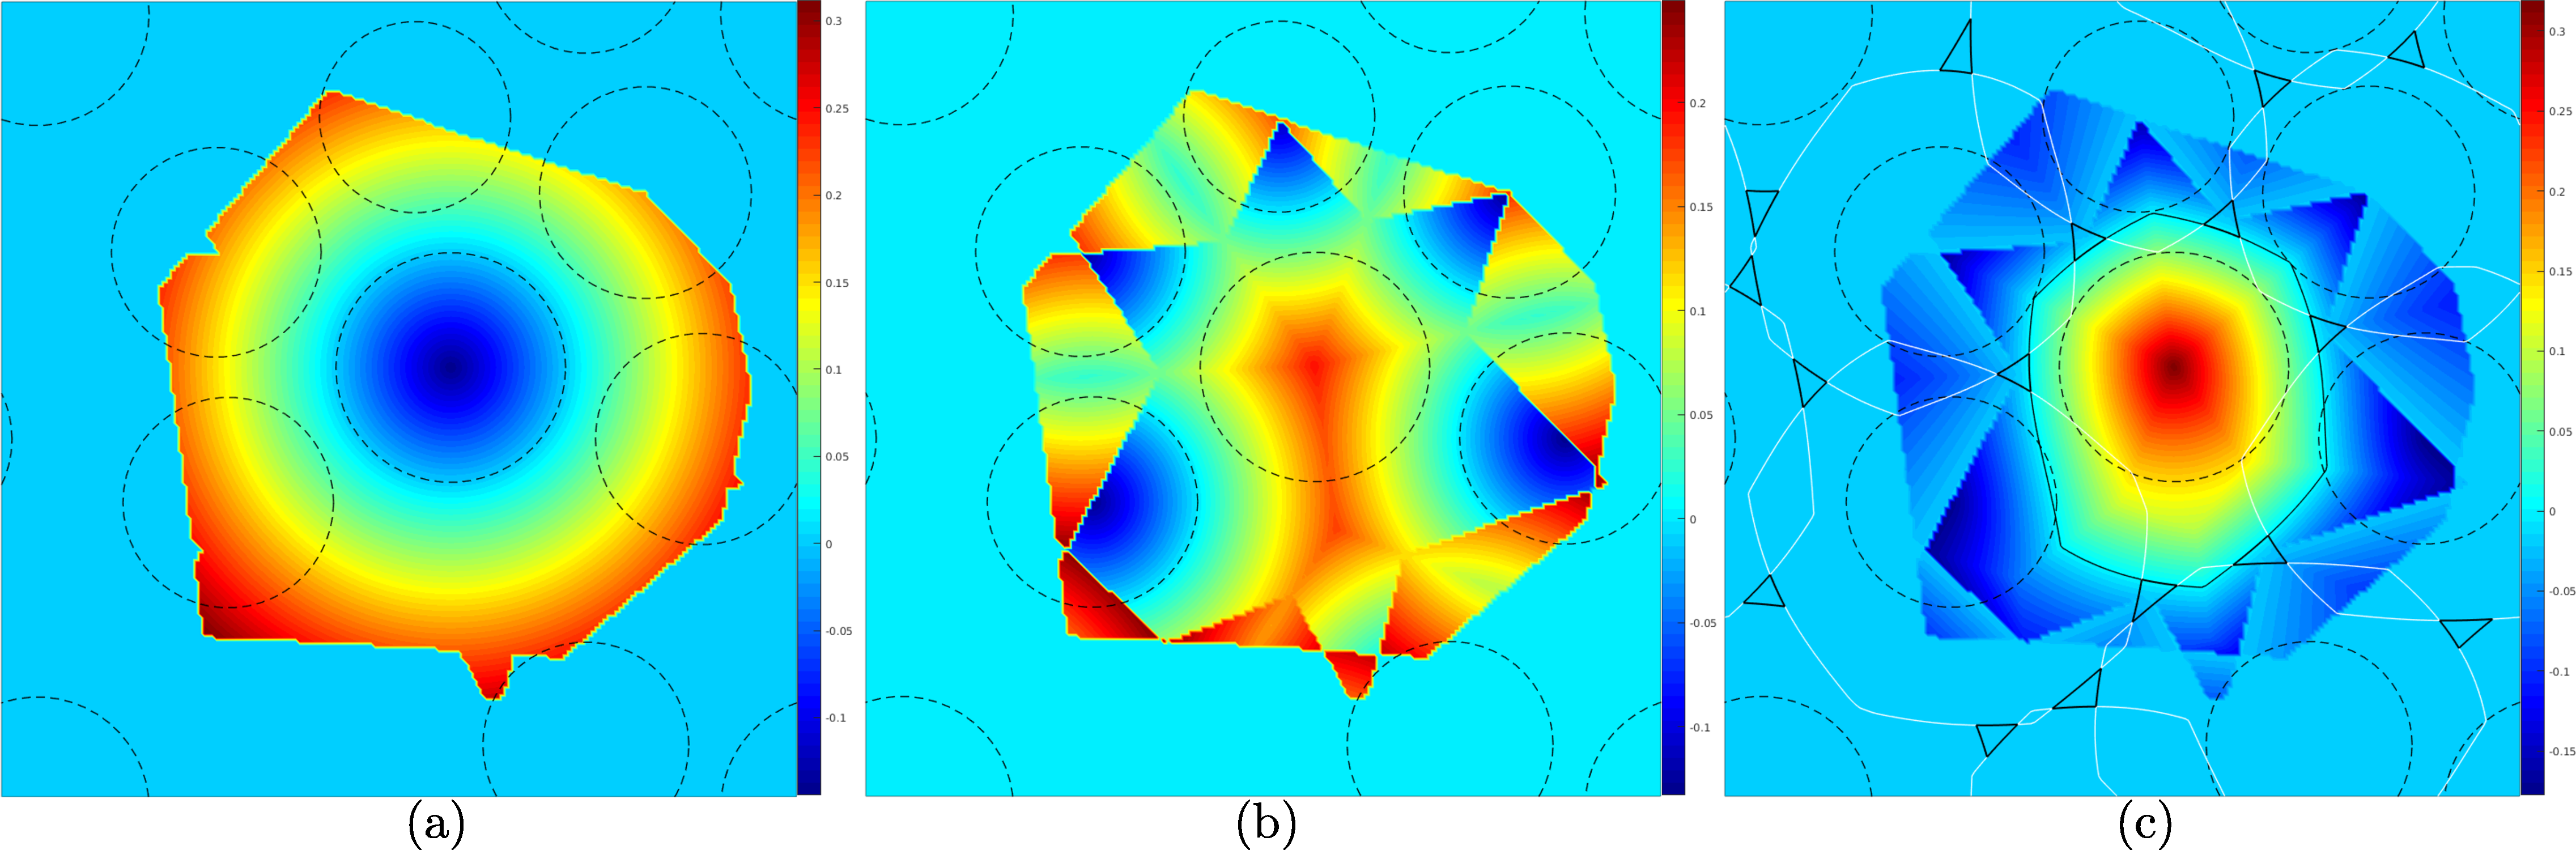
\includegraphics[height=5cm]{inner}
	\caption{(a) Modified ``local'' $ ^IDN_{1i} $ function, and (b) modified ``local'' $ ^IDN_{2i} $ function, for inclusion $i$. The difference with the global functions plotted in Figure \ref{dn1} can be seen by comparison. (c) $ ^IO_{Pi} $ function for inclusion $i$ is plotted with the $ t $ level set drawn in black, while those of the immediate neighbors are drawn in dotted white. The triangular slices that form the part of the global $ t $ level set have also been plotted in bold white for reference. }\label{inner4}
\end{figure}

It should be noted that the operators necessary for introducing ligament curvature and strut cross-section variation can be built globally and used in a straight-forward manner along with the local $ ^IDN_{ki} $ functions. Also, a significant computation cost can be saved by limiting the computation domain to a band enclosing the surface to extract, which can be identified with the help of the $ NN_k $ functions:
\begin{equation}
\begin{split}
DOI_i&\equiv\left(\left(NN_1(\textbf{x})=i\right)|\left(NN_2(\textbf{x})=i\right)|\left(NN_3(\textbf{x})=i\right)\right)\\
&\&\left(\left(O_V(\textbf{x})-t>-e\right)\&\left(O_V(\textbf{x})-t<e\right)\right)\,,
\end{split}
\end{equation}
where $ e=t/2 $ and is at least twice the discretization size of the domain.
Figure \ref{sharp1}c illustrates the extraction of an RVE by the help of multiple level sets with the desired features.

\section{Finite element mesh generation}\label{of-fem}

For use in a computational simulation, it is necessary to generate the volume discretization of the geometries obtained from the level set functions discussed before. For this purpose, a simple mesh generator is used that takes into account the slicing operations while giving a consistent discretization along the sharp edges. The tool developed in \cite{ehabmoustafakamelIntegratedApproachConformal2019} is therefore used, where dynamic node repositioning based on level set functions is used to build high quality conforming meshes using the strategy developed in \cite{perssonSimpleMeshGenerator2004}. A similar strategy has been used in \cite{wintibaAutomatedProcedureGeneration2017} to generate textile reinforced composites RVEs.

The sharp edges can be extracted from the intersecting surfaces extracted from the definition of $ ^IO_P $ of two adjacent inclusions using any of the standard Boolean operations on surfaces, like the triangle/triangle intersection test routine \cite{mollerFastTriangleTriangleIntersection1997}, or the Boolean operation tool on 3D polyhedra \cite{bernsteinFastExactLinear2009}. For any two adjacent inclusions, the surface extracted using the intersection approach is a combination of the two sliced surfaces sharing a common curve representing the sharp edge (Figures \ref{intersect2}a and b). 

\begin{figure}
	\centering
	\begin{subfigure}[b]{0.35\textwidth}
		\includegraphics[width=\textwidth]{edge_surf}
		\caption{}
	\end{subfigure}
	\begin{subfigure}[b]{0.62\textwidth}
		\includegraphics[width=\textwidth]{edge_mesh}
		\caption{}
	\end{subfigure}
	\caption{(a) Common curve extracted from the intersection of the surfaces obtained from $ ^IO_P $ function of two adjacent inclusions. (b) The re-meshing of the common curve of intersection using a piece wise cubic Hermite polynomial interpolation. The red dots represent the nodes being remeshed.}\label{intersect2}
\end{figure}

The standard approach to extract triangulated surfaces from discrete points in a grid is to use the isosurface technique based on the marching cube method developed by Loreson and Cline \cite{lorensenMarchingCubesHigh1987} according to a pre-specified variable target size function, $ h(\textbf{x}) $. The triangulated surfaces constructed can then be used as a constraint towards tetrahedral mesh generation  by 3D Delaunay Triangulation. The Constrained Delaunay Triangulation (CDT \cite{shewchukConstrainedDelaunayTetrahedralizations2002}) module implemented in the software Tetgen \cite{siTetGenDelaunayBasedQuality2015} is used to obtain a conformal mesh for which the constraint ensures that the output contains the faces of surfaces discretizing the material boundaries while preventing elements to span across material boundary interfaces. As a Delaunay mesh generator, Tetgen accepts a predefined surface mesh in the form of polyhedrons, known as Piecewise Linear Complex (PLC).

% Remarks
However, this approach, when used directly, leads to a notable presence of ill-shaped faces (too small, too narrow, etc) resulting from the initial surfaces extracted from the isosurface technique. It is therefore unfit for a proper use in finite element computations. To overcome this, a mesh quality optimization process is applied on the mesh. The common curves representing the sharp edges are re-interpolated initially based on  $ h(\textbf{x}) $ (Figure \ref{intersect2}) and then the surface elements of the isosurfaces are re-triangulated keeping this re-interpolated curve of the sharp edge fixed (Figure \ref{fig:surf_smooth}). 
\begin{figure}
	\centering
	\begin{subfigure}[b]{0.45\textwidth}
		\includegraphics[width=\textwidth]{surf_rough}
		\caption{}
	\end{subfigure}
	\begin{subfigure}[b]{0.45\textwidth}
		\includegraphics[width=\textwidth]{smooth_surf}
		\caption{}
	\end{subfigure}
	\caption{(a) Surface extracted from $ ^IO_P $, sliced and common curves re-interpolated. (b) Surface after optimization by force based tensioning scheme.}\label{fig:surf_smooth}
\end{figure}

The ideal situation of a high quality mesh, i.e., the presence of only quasi-regular tetrahedra with edge lengths $ l^e $ equal to the value of the targeted element size map $ h(\textbf{x}_e) $ at corresponding edge mid points $ \textbf{x}_e $, cannot be reached exactly for complex RVEs and varying element sizes. However, configurations (or node positions) can be found that minimize the magnitude of the difference, 
\begin{equation}
F^e=l^e-h(\textbf{x}_e),\label{truss-eqn}
\end{equation}
over the mesh, which helps obtaining optimal element quality for a given triangulation. The methodology for mesh optimization follows an original idea used in \cite{perssonSimpleMeshGenerator2004} where an analogy with the equilibrium configuration of a 3D truss of elastic bars is applied to the optimization of the edges of the tetrahedral mesh. This methodology was recently extended to heterogeneous micro-structures in \cite{ehabmoustafakamelIntegratedApproachConformal2019}. The bars of this auxiliary truss are subjected to a force $ \textbf{f}^e $ acting along the bars, proportional to $ F^e $ in Eq. (\ref{truss-eqn}). These forces cancel out at the nodes by mechanical equilibrium. This procedure is equivalent to the application of an internal force field steering the lengths of the truss bars towards $h(\textbf{x})$. A fictitious resultant force $ \textbf{f}(\textbf{x}_n) $ is defined that acts on all nodes positions that need to be optimized. This force is simply the vectorial sum of $ \textbf{f}^e $ acting on all such nodes and thus, for a given triangulation, equilibrium requires
\begin{equation}
\textbf{f}(\textbf{x}_n)=0.\label{truss-equi}
\end{equation} 
This condition corresponds to the optimal node positions $ \textbf{x}_n $ as the result of a fictitious mechanical equilibrium. A fictitious time dependency can be introduced to solve this equations system,
\begin{equation}
\frac{\text{d}\textbf{x}_n(t)}{\text{d}t}=\textbf{f}(\textbf{x}_n) ,
\end{equation}
along with a forward first order Euler time integration scheme,
\begin{equation} \textbf{x}_n(t+\text{d}t)=\textbf{x}_n(t)+\text{d}t\,\textbf{f}(\textbf{x}_n)  ,
\end{equation}
to reach a stationary state from the base mesh based on a defined tolerance. 

When meshing and optimizing the three different outer surfaces of the foam struts, it is important to ensure that the nodes located on the common sharp edges remain fixed. Subsequently, when meshing the strut volumes, surface nodes are kept fixed using the already stored level set information. The nodes lying on the RVE boundary faces are treated to ensure that they remain on the faces and satisfy any periodicity conditions applied. In practice, to ensure robustness and versatility, the optimization process is thus applied on the extracted sliced isosurfaces and the RVE faces first followed by CDT, with the optimized surface acting as the constraint. This step of global optimization leaves the already optimized nodes untouched. Note that a similar force-based approach could also be implemented to optimize the common sharp edges before meshing the surfaces instead of a simple re-interpolation. 

\red{The distance fields that store the implicit description of the geometry are used at this stage to ensure that the topology of the strut geometry resulting from one of the three inclusions does not change. The information obtained through the distance functions like the complex geometrical description, distance to neighbors, curvature, etc., provides sufficient details to handle complex topologies. Considering that the sharp edges are fixed, the surfaces of the inclusions can be meshed and optimized independently, while ensuring that the optimized surface triangles are ``locked" to the original surface. The nodes that lie on the inclusion surface, but not on the sharp edges are moved around while respecting the level-set value prescribed at the time of initial inclusion extraction. The network of edges formed by these nodes are repeatedly swapped to ensure minimum distortion to the overall topology. This simplifies the problem before producing a volume triangulation using Tetgen. This procedure is explained further in \cite{ehabmoustafakamelIntegratedApproachConformal2019}. A similar process has also been extended to the surfaces that lie on the boundary where the nodes from the sharp edges, as well as the edges from the previously optimized inclusion surfaces are ``locked''.}

Figure \ref{fig:model_smooth} illustrates a portion of the RVE before and after surface optimization. Figure \ref{fig:tetra_section} illustrates a portion of the RVE after the CDT process and a sectional view of the tetrahedrals.  

\begin{figure}
	\centering
	\begin{subfigure}[b]{0.45\textwidth}
		\includegraphics[width=\textwidth]{model_coarse}
		\caption{}
	\end{subfigure}
	\begin{subfigure}[b]{0.45\textwidth}
		\includegraphics[width=\textwidth]{model_fine}
		\caption{}
	\end{subfigure}
	\caption{Sectional representation of an RVE generated by DN-RSA (a) before, and (b) after surface mesh optimization process.}\label{fig:model_smooth}
\end{figure}

\begin{figure}
	\centering
	\begin{subfigure}[b]{0.65\textwidth}
		\includegraphics[width=\textwidth]{tetra_model_slice}

	\end{subfigure}
	\caption{Conformed 3D mesh made of tetrahedrals after CDT process using Tetgen.}\label{fig:tetra_section}
\end{figure}

\section{Conclusions}
A detailed methodology to produce a representative volume element of a random open foam metallic structure using distance fields and level sets has been presented in this chapter. An open foam geometry generation algorithm presented in an earlier work has been extended upon to extract RVEs that are expected to be morphologically similar in a quantitative way to that of real open foam samples in terms of the randomness in the geometry of the inclusions, the variation of the strut geometry and the presence of other uncertainties in the extracted model. This methodology has also been extended to a geometry reconstruction process where polyhedrals that conform to the pores of the open foam material extracted from CT-scan images has been substituted to the inclusion packing algorithm. This process enables one to proceed with geometry reconstruction with the necessary geometrical tweaking capabilities enabled by the calculated distance fields.

Starting from the packing algorithm presented in \cite{sononUnifiedLevelSet2012} and operators presented in \cite{sononAdvancedApproachGeneration2015}, additional modifications have been proposed to generate more subtle shapes of the strut geometry, and to achieve the randomness existing in the real materials, like  strut cross-section variation with axis and concavity in the strut cross-section. Finally, further exploiting the advanced mesh generation tools presented in \cite{ehabmoustafakamelIntegratedApproachConformal2019}, a methodology to extract a finite element model from the implicit geometry has been presented.

The methodology presented to generate random volume element needs to be verified statistically for the extracted meshes to be utilized in a computational homogenization procedure explained in Chapter \ref{chap-ch}. A discussion on the statistical validity along with the material response to loading conditions will be presented in Chapter \ref{chap-res}.

\red{The versatility of the tool can be further complemented by implementing grid point based morphology variation. Currently, the versatility is restricted to features such as uniform strut geometry across the morphology that depends only on the value of the distance fields from which it is extracted and a scalar control based open / close pore faces. Nevertheless, it can be extended to other feature controls too. These can be in the form of strut thickness variation depending on the position of the struts in the geometry, additional controls on open / close faces of the pores, accumulation of material at the nodes and so on. However, to conduct a critical implementation of these complexities, additional experimental data is necessary that can help in statistically implementing them, which is currently lacking. }


